% USC Dissertation/Thesis LaTeX Template
% Edited by Ruda Zhang, 2020-10-08.
% -----------------------------------------------------------------------------
%	PACKAGES AND DOCUMENT CONFIGURATION
%-----------------------------------------------------------------------------

% Use `report` class with `USCthesis` package (style file) by Brian P. Gerkey
% Font size should be 11 or 12 points for regular paragraph text.
\documentclass[letterpaper,12pt]{report}
% [options] can be any of these default/alternative flag:
%   dissertation/thesis, final/proposal, copyright/nocopyright,
%   fussy/sloppy, flushbottom/raggedbottom, clref/opref.
\usepackage[dissertation, final, opref, raggedbottom]{USCthesis}

% Packages required by `USCthesis.sty`.
\usepackage{hyperref}
\usepackage{setspace}
\usepackage{tabularx}
\newenvironment{myepigraph}
  {\par\hfill\itshape
   \begin{tabular}{@{}r@{\hspace{2em}}}} % 2em from the right margin
  {\end{tabular}\par\medskip}

% Line spacing and margins in compliance with USC graduate school guidelines.
\usepackage[margin=1in,footskip=.5in]{geometry}
\doublespacing

% Optional packages: mathematical fonts and symbols
% You may comment this section out if you don't need them.
\usepackage{mathptmx} % set font to Times Roman
\usepackage[OT1]{fontenc} % font encoding for xelatex
\usepackage{mathtools}
\usepackage{amsmath}
\usepackage{amssymb}

% Optional packages: graphics
\usepackage{graphicx}
% You can use the "demo" option while editing to avoid compiling figures.
% \usepackage[demo]{graphicx}
% You can add absolute paths as well.
\graphicspath{{./}{../}{figures/}{../figures/}{main/rvagene/figures}}
% Optional packages: bibliography with BibLaTeX.
% Comment this section out if you prefer BibTeX.
%\usepackage[
%    style=nature,
%    sorting=none,
%    isbn=false,
%    url=false,
%    doi=true,
%    eprint=false,
%    date=year,
%    maxnames=6,
%    minnames=6
%]{biblatex}
%\AtEveryBibitem{\clearfield{eventtitle}} 
%\AtEveryCitekey{\clearfield{eventtitle}}
%\AtEveryBibitem{\clearfield{pagetotal}} 
%\AtEveryCitekey{\clearfield{pagetotal}}
%\addbibresource{references.bib}


% Filler text for formatting. Comment these lines out for real writing.
\usepackage[english]{babel}
\usepackage{blindtext}
%%%%%%%%%%%%%%% My Additions ############

%\usepackage[top=0.85in,left=2.75in,footskip=0.75in,marginparwidth=2in]{geometry}
\usepackage{pmi} %pmi piyush rai style
%\usepackage{ml}
% use Unicode characters - try changing the option if you run into troubles with special characters (e.g. umlauts)
\usepackage[utf8]{inputenc}
\usepackage[lining,semibold]{libertine} % a bit lighter than Times--no osf in math
\usepackage[varqu,varl]{inconsolata}% a typewriter font must be defined
% clean citations
%\usepackage{cite}
% hyperref makes references clicky. use \url{www.example.com} or \href{www.example.com}{description} to add a clicky url
\usepackage{nameref,hyperref}
\hypersetup{
  colorlinks   = true, %Colours links instead of ugly boxes
  urlcolor     = blue, %Colour for external hyperlinks
  linkcolor    = blue, %Colour of internal links
  citecolor    = blue  %Colour of citations
}
% line numbers
\usepackage[right]{lineno}
\newcommand\numberthis{\addtocounter{equation}{1}\tag{\theequation}}

% improves typesetting in LaTeX
\usepackage{microtype}
\DisableLigatures[f]{encoding = *, family = *  }
\usepackage{wrapfig}

% text layout - change as needed
%-------------------------------------------------
% \raggedright
% \setlength{\parindent}{0.5cm}
% \textwidth 5.25in
% \textheight 8.75in
%--------------------------------------------------
% Remove % for double line spacing
%\usepackage{setspace}
%\doublespacing

% use adjustwidth environment to exceed text width (see examples in text)
\usepackage{changepage}

% adjust caption style
\usepackage[aboveskip=1pt,labelfont=bf,labelsep=period,singlelinecheck=off]{caption}


\makeatletter
\renewcommand{\@biblabel}[1]{\quad#1.}
\makeatother
\usepackage[backend=biber, style=numeric, sortcites, maxnames=10, natbib=true]{biblatex}
\usepackage{csquotes}% Recommended
\usepackage{pmi}
%\bibliography{library}
\addbibresource{library.bib}
\newcommand{\tcr} { \textcolor{red} }

\newcommand{\scrna}{scRNA-seq }

\makeatletter
\renewenvironment{abstract}{%
  \if@twocolumn
    \section*{\abstractname}%
  \else
    \small
    \begin{center}%
      {\bfseries \abstractname\vspace{-.5em}\vspace{\z@}}%
    \end{center}%
    \quotation
  \fi}
  {\if@twocolumn\else\endquotation\fi}
\makeatother


\begin{document}

%-----------------------------------------------------------------------------
%	TITLE PAGE
%-----------------------------------------------------------------------------

% Volume name could be added as option, e.g. `[Volume I]`.
\title{\textbf{\Large{Deciphering Protein-Nucleic Acid Interactions with Artificial Intelligence}}}

\author{Raktim Mitra}

% Committee list is only shown in `proposal` layout.
\committee{A.~Remo Rohs & (Chair)\\*
           B.~Adam MacLean\\*
           C.~Fengzhu Sun\\*
           D.~Helen Berman \\*
           E.~Aiichiro Nakano & (Outside Member)}

% Submission information is only shown in `final` layout.
\majorfield{Computational Biology and Bioinformatics}
\submitdate{December 2024}  % Must be one of the three dates allowed in the guideline

% Make sure everything, specially your title page, exactly follows the guideline:
% https://graduateschool.usc.edu/wp-content/themes/fictional-university-theme/assets/doc/Manuscript_Formatting_and_Documentation_Styles.pdf

%-----------------------------------------------------------------------------
%	PREFACE
%-----------------------------------------------------------------------------

% The preface environment prints the title page.
\begin{preface}

  \prefacesection[Epigraph]{Epigraph}
  \topskip0pt
\vspace*{\fill}
\vspace*{-2in}
\begin{myepigraph}
\large
``Karmanye v$\bar{\text a}$dhik$\bar{\text a}$raste M$\bar{\text a}$ Phaleshu Kad$\bar{\text a}$chana,\\ 
\large 
M$\bar{\text a}$ Karmaphalaheturbh$\bar{\text u}$rm$\bar{\text a}$ Te Sangostvakarmani."\\
\large $-$Srimadbhagabatgita,  S$\bar{\text a}$nkhya Yoga (Dwitiya Adhyaya), Sloka 47
\end{myepigraph}
%\epigraph{Karmanye vadhikaraste Ma Phaleshu Kadachana,\\ Ma Karmaphalaheturbhurma Te Sangostvakarmani}{Srimadbhagabatgita,  Sānkhya Yoga (47) }
\vspace*{\fill}
  % Dedication Page, which is truly unnecessary.
  \prefacesection[Dedication]{Dedication}
  \topskip0pt
\vspace*{\fill}
\vspace*{-2in}
\begin{quote}
    \center
    I dedicate this thesis to $x$ and $y$, \\
    for their never ending mysteries.
\end{quote}
\vspace*{\fill}


  % Acknowledgement Page, which is also unnecessary for proposals.
  \prefacesection{Acknowledgements}
  %% CHANGE NAMES AND WRITING

I offer my utmost thanks to my advisor Prof. Remo Rohs, whose encouragement, patience, intelligent decisions and immense knowledge supported me throughout my Ph.D., made it a wonderful experience, and helped me overcome many difficulties.

I am also extremely thankful to my dissertation committee members Prof. Helen M. Berman, Prof. Fengzhu Sun, Prof. Adam L. MacLean and Prof. Aiichiro Nakano, and qualifying exam committee member Prof. Xiaojiang Chen. Their insightful comments enriched and widened my research from various perspectives. Also, thanks to Prof. Adam L. MacLean, for working with me in my first rotation and afterwards, to help me publish my first first-author paper.

I also present my gratitude to my collaborator Dr. Cameron Glasscock from the David Baker lab at University of Washington, and to Prof. Ada Yonath and her lab members, for being supportive to my research. 

I am thankful to the Andrew Viterbi Fellowship in Computational Biology and Bioinformatics for supporting me over three years of my PhD.

My sincere thanks goes to the QCB department for allowing me to participate in various departmental acitivities which helped shape me as a person. It has been a pleasure to work with and receive all forms of support from Rokas, Tanya, Katie and Christian.

I thank my fellow labmates Yibei, Tsu-pei, Jinsen, Ari, Jesse, Yingfei, George, previous lab members Brendon and Jared. This dissertation would not have been possible without their stimulating discussions and contributions, both in science and in life. Specially, without Jared's mentorship during the earlier years of my PhD, my dissertation would not be able to achieve its current form. I also thank my graduate mentees Zijin, Wei, Chan, Lexi (and others), and my undergraduate mentees Andrew, Hirad, Avinash and Irika. It has been a pleasure to work with all of you and to see your scientific growth. 
Special thanks go to my friends Bryan, Meilu, Sophia, Vivian, Fred, Eric, Priyanka, Chloe, Nic and Anik, for supporting me along the way. You have made my life in Los Angeles a pristine remembrance. I also offer my gratitude to Prof. Lina Bahn, Christine Lee, Yue Qian, and Haesol Lee, for helping me pursue my interest in violin and music, which helped me conquer many challenging times.

Last but not the least, I am forever indebted to my parents without whose decades long hard work and dedication I would not even be here. On the same thread, I am grateful for the support of my extended family members and childhood friends and teachers, who provided me with unfailing support and continuous encouragement throughout the journey.
{
  \hypersetup{linkcolor=black}
  \tableofcontents
  %\listoftables   % Comment this out if you don't have tables
  \listoffigures*
}

  % Abstract Page
  \prefacesection{Abstract}
  This dissertation proposal contains an account of my research work so far, a proposed next project and discussion about possible future work.
Applying probabilistic machine learning models to solve biological questions has been my primary focus as a researcher. 
In chapter 1, we design and showcase RVAgene: a recurrent variational
autoencoder model applicable on gene expression time-series data, to learn a regularized latent
space representation and a generative process. RVAgene is primarily a visualization tool suitable for biological 
knowledge discovery, while also being suitable for de novo data generation, denoising and a more
efficient alternative to hierarchical Gaussian process based methods to cluster such data. We
analyze one synthetic and two real datasets and demonstrate various properties and aspects of the
model and its potential for unsupervised discovery.  In particular, RVAgene identifies new programs of 
shared gene regulation of \textit{Lox} family genes in response to kidney injury. In
chapter 2, we deal with a different biological problem, using the same probabilistic modeling
technique of Bayesian Variational Inference (VI). Here, we start from a model of nucleic acid binding site
prediction (Geobind) developed by Jared Sagendorf and improve upon it by designing a neural network layer using mean field
VI over a continuous Conditional Random Field model, which makes the predicted binding sites
smoother while improving upon prediction metrics. We also design a smoothness metric
addressing the label imbalance problem associated with the task. In chapter 3, we focus on the fact that the Geobind
model for binding site prediction does not take into account information regarding the binding
elements (drug molecules or nucleic acid sequences). The reason is, for a discriminative model like
Geobind, the datasets become very sparse if we aim to train on datasets specific to nucleic acid
sequences. However, a generative model inspired by and similar to RVAgene can be useful in this
scenario. So, we start where Geobind ends. We propose a generalized binding element design model, where we take binding site
information or some region of interest on a protein surface as input, and generate binding elements which
could bind to the given region of interest on a protein surface. Finally, in chapter 4, we conclude
this dissertation proposal while discussing some long term project ideas for future work.

\end{preface}

%-----------------------------------------------------------------------------
%	CONTENT STRUCTURE
%-----------------------------------------------------------------------------

% Better to separate LaTeX structure and content


%%%%%%%%%%%%%%%%%%%%%%%%%%%%%%%%%%%%%%%%%%%%%%%%%% CRF %%%%%%%%%%%%%%%%%%%%%%%%%%%%%%%%%%%%%%%%%%%%%%%%%%%%%%%%%%%%%%%%%%%%%%%%%%%
% More Research Topics
% \include{ResearchTopic2}

\chapter{A probabilistic model for smooth binding site label prediction on protein surfaces}
\label{cha:research_topic_2}

\vspace*{0.35in}

\begin{flushleft}

%{\large Raktim Mitra\textsuperscript{1}, 
%Jared Sagendorf\textsuperscript{1}}\\

%\bigskip
%$^1$Quantitative and Computational Biology, University of Southern California
%\\


\end{flushleft}

%\begin{abstract} 
    Predicting DNA/RNA binding sites on a given protein surface is an important computational task, since experimentally determining such information is often expensive and time consuming. This binding site prediction task can be formulated as a node classification task over a 3D mesh representing the protein surface, with features over the vertices and edges of the mesh representing various geometrical and physicochemical features of the protein structure. We developed a deep learning based method, PNAbind, which classifies mesh vertices as binding and non-binding sites. This often results in irregular binding site predictions over the protein surface. However, intuitively, binding site predictions should be contiguous and not patchy i.e. as ``smooth" as possible while being correct. In this chapter, we describe what such kind of ``smoothness" entails and we improve upon the original architecture by designing a network layer based on a probabilistic Continuous Conditional Random Field (CCRF) model, which increases smoothness of binding site prediction while improving prediction accuracy of the model. This network layer implementation has been published as part of the PNAbind package.
\end{abstract}

%\section{Introduction} Predicting DNA/RNA binding sites on protein structures is an important
computational task.  There are many existing methods which attempt to solve this problem either on
the sequence level or on 3D structure level based on either sequence features or structural features
of proteins \citep{deng2018pdrlgb, wang2010bindn+, wang2006bindn, li2013predna}
.We  represent protein surfaces as 3D triangulated meshes with 
vertices and edges having features representing diffferent geometrical and physicochemical aspects
of the protein structure. Now, we can learn a model which classifies each vertex of such a mesh to either binding-site or
non-binding sites. With recent advances in 3D deep learning, Graph Convolutional
Networks(GCNs) have come out as a useful approach for learning higher level features over
3D mesh objects. We developed a GCN based deep learning model for the binding site classification
task: Geobind. \hyperref[fig:crf_concept]{Fig. 2.1A} shows schematic diagram of
the task Geobind achieves.

Standard neural network approach is to predict each binding-site label independently
through it's output layer. However, classification tasks often come with additional non-trivialities which
are not addressable with independence assumption.  For example, image segmentation task involves
classifying every pixel of an image (which can be thought of as a grid of pixels) to some class.
However, independence assumption often gives poor/scattered results. In that case, some form of
conditionallabel (re)assignment is necessary for each pixel considering its neighbouring pixels. The
most common way to achieve the same in the field of computer vision is via optimizing a conditional
random  field (CRF) model over a set of initially  learned labels. For example,
\hyperref[fig:crf_concept]{Fig. 2.1B} adapted
from \citet{krahenbuhl2012efficient}  shows how an implementation based on CRF can improve image
segmentatation results. In our case, we also expect certain properties from a predicted binding site
region on a protein surface. A binding site region on a protein surface is basically a combination
of multiple mesh vertices predicted as binding site. We generally expect such a region to be
"smooth" i.e. not randomly have misclassified points scattered around. This idea is visually illustrated in
\hyperref[fig:crf_concept]{Fig. 2.1C}. So, we need to do some kind
of conditional (re)assignment of class labels generated by our Geobind network.

In addition to Computer vision, CRF models are also heavily used in Natural Language processing (NLP)
\citep{roark2004discriminative,mccallum2003early,liu2017identification}. However, both in Computer
vision and NLP, the underlying graph structure, over which the CRF is defined, is very sparse and
simple e.g. linear chain or tree for NLP and 2D grid for computer vision. Which makes it easy to
find some form of optimization scheme on the discrete domain of labels. However, this is not the
case for a general underlying graph, where the combinatoriality of the possible label assignments
for all vertices is huge and in the discrete domain of labels there is no gradient information for
efficient optimization.

\citet{krahenbuhl2012efficient} proposes an efficient inference algorithm for fully connected CRFs
based on mean field Variational Inference and high dimensional filtering using permutohedral lattice
approximation. However, the high dimensional filtering step is not compatible with
SIMD\citep{nickolls2008scalable} paradigm of GPU computation. \citep{teichmann2018convolutional}
making it impossible to use on large datasets and non-trivial graphs.
\citet{teichmann2018convolutional} improves upon this by implementing Convolutional CRFs which is
another kind of approximation to full CRF inference which is efficient and compatible with GPUs.
However, their method is only applicable for 2D grid i.e. image data.  However, none of these methods
are applicable to our case directly. One of the more interesting advances of applying CRF layer on
mesh object comes from \citet{kalogerakis2010learning} using alpha-expansion graph-cuts method proposed by
\citet{boykov2001fast}. However, being pre-CNN revolution work, this method is not sutiable for deep
learning and is not readily integrable to our Geobind model. 
\par
Overall, it turns out, optimizing a CRF model over the predicted labels of Geobind on the discrete
domain to reassign them is not computationally easy. However, instead of trying to smooth the
predicted labels we can directly try to make these predicted labels itself smoother. This means we
need to have an operation before the final fully connected layer of Geobind which smooths the
information over different vertices taking into account their neighbours information along with
their own. The good thing about this idea is that the optimization domain is not discrete anymore.

Such an operation is based on Continuous variant of a CRF or CCRF. \citet{ristovski2013continuous}
shows how to calculate the updates for such a model using mean field variational inference, although
not in a neural network context. \citet{gao2019conditional} introduces this approach for graph
convolution based networks, however, the network layer update equation presented in their work is
faulty and results into simply an Identity transaformation. We calculated the correct
form of the network layer which we use as the second last layer of our Geobind model.

In this next sections we shall formally describe a metric  denoting "smoothness" of binding site
prediction over protein meshes, the CCRF model and the CCRF layer's architecture, followed
by results showing how it has significantly improved Geobind for the binding site classification task.
\begin{center} 
 \begin{figure}[!htp]
                \makebox[\textwidth]{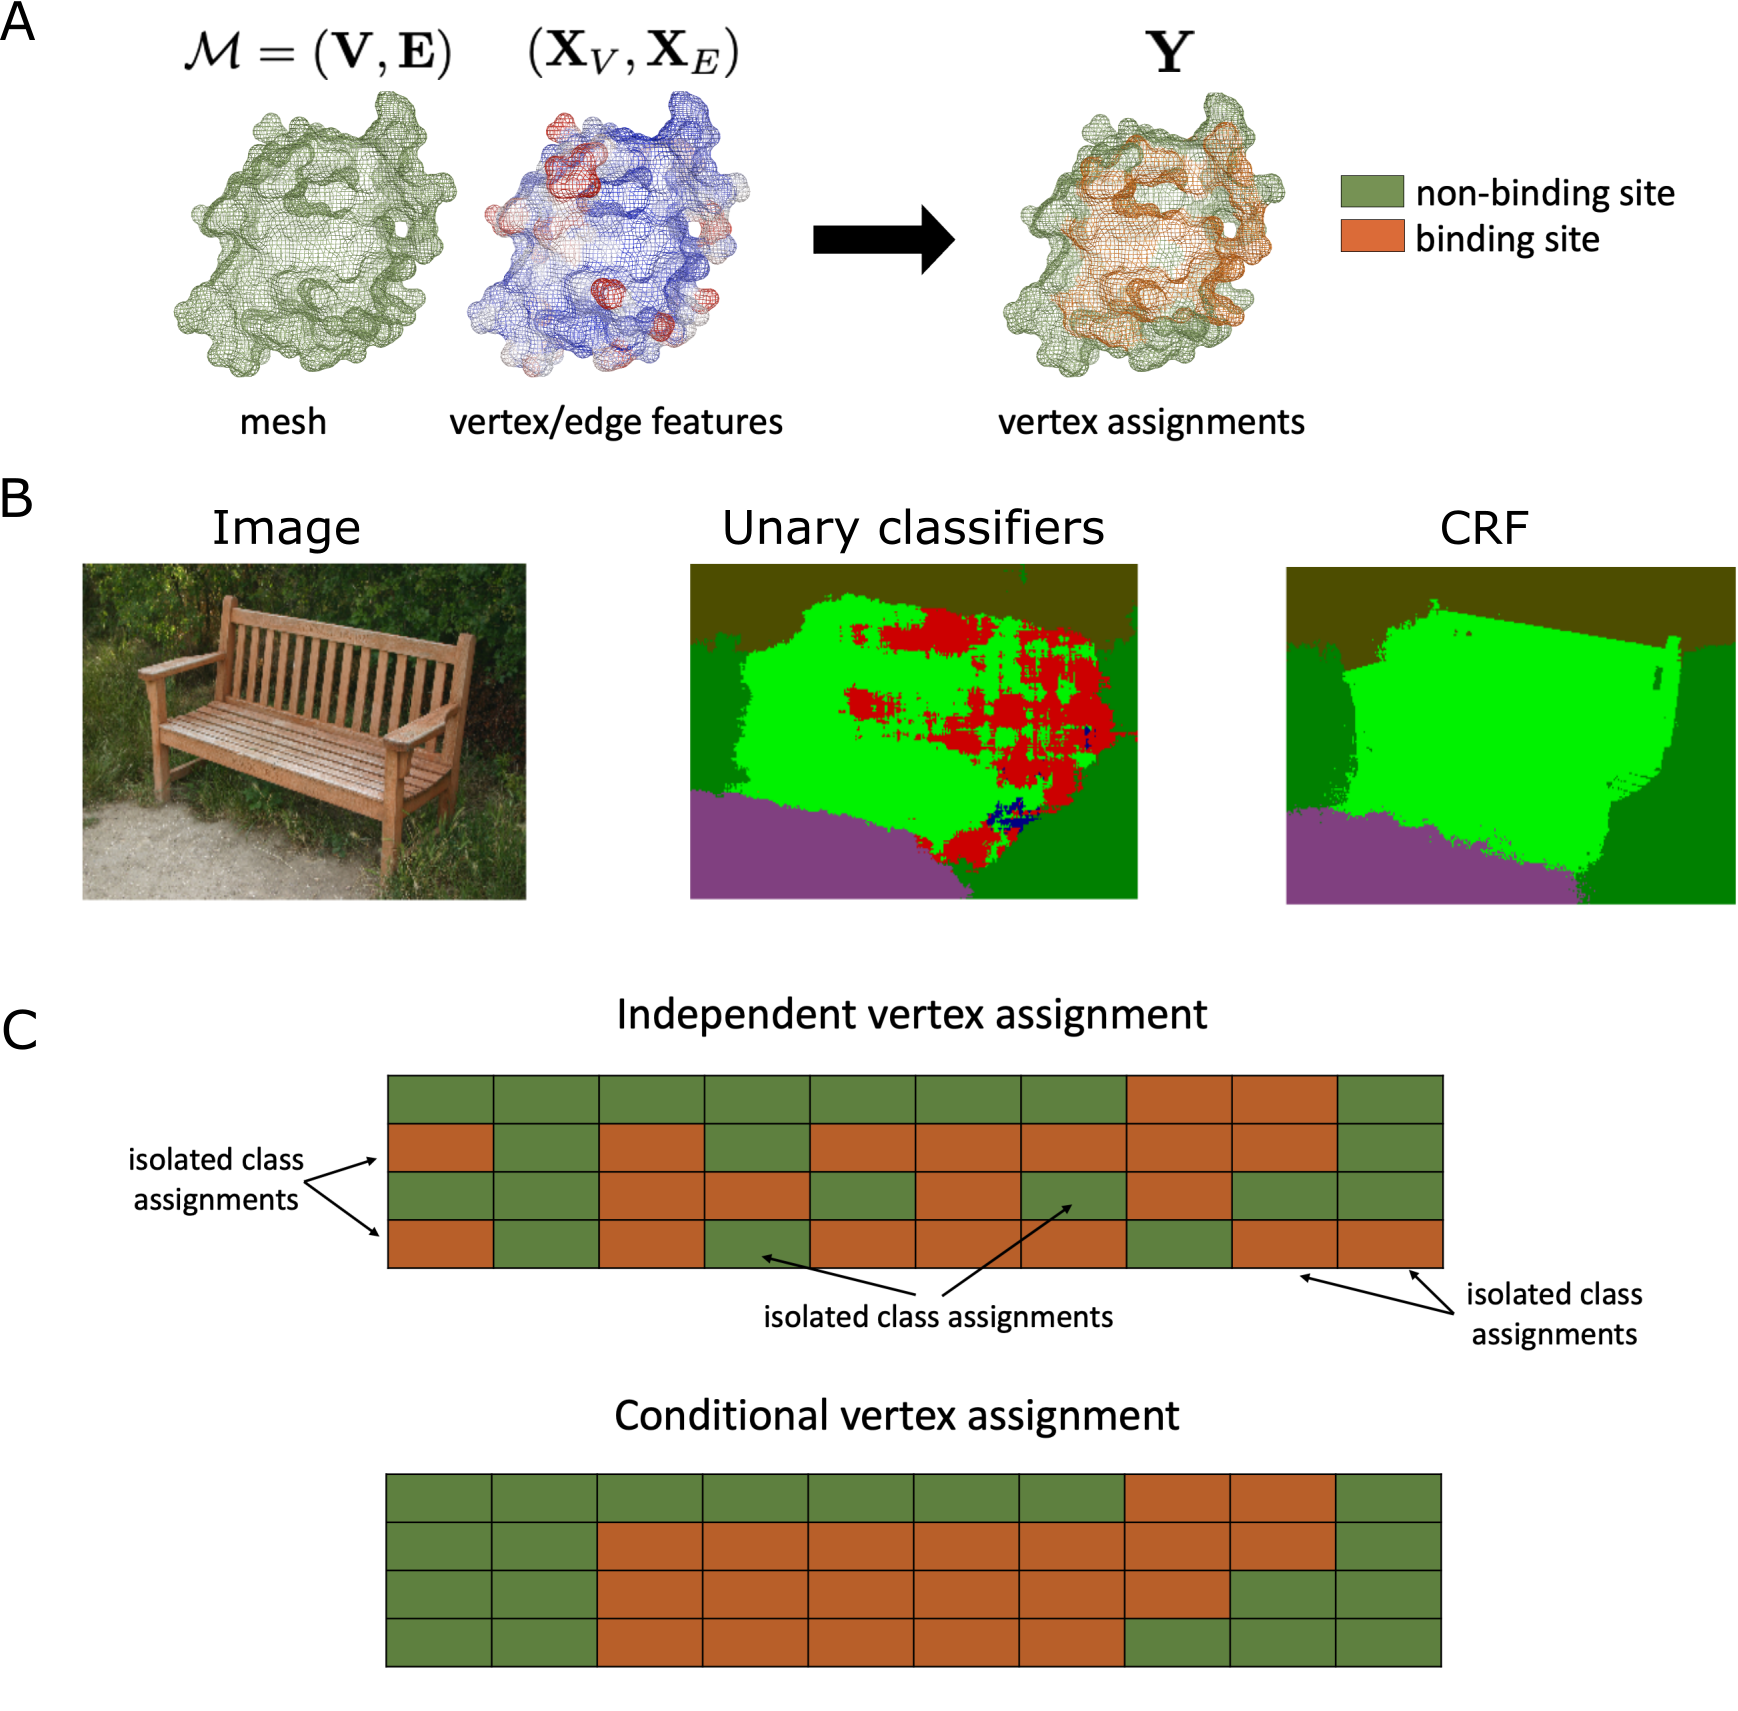
\includegraphics[width=0.8\paperwidth]{crf_figs/crf_concept.png}}
 % archetecture.png: 1149x508 px, 72dpi, 40.53x17.92 cm, bb=0 0 1149 508
        \caption[Geobind schematic, example and conceptual explanation of CRF application scenario]{\textbf{Geobind schematic, example and conceptual explanation of CRF application scenario}
        ({\bf A}) Schematic diagram showing how Geobind predicts binding sites over a protein surface represented as a mesh. ({\bf B}) \citet{krahenbuhl2012efficient} shows how applying a fully connected CRF model results in better image segmentation results compared to 
        just unary classification. ({\bf C}) (above) An exmple independent class assignment in a 2-D grid of cells which is irregular, (below) A smoother classification, which we would 
        expect to get as result of a conditional assignment process.}
        \label{fig:crf_concept} \end{figure} \end{center}

%\section{Methods}
We develop a recurrent variational autoencoder to model gene expression dynamics (RVAgene). Here we briefly describe the methods underpinning variational autoencoders, and present the implementation of RVAgene. 

\subsection{Variational inference and variational autoencoders}
In the most general setting of a Bayesian model, we seek to learn the latent variables $\vz$ that best characterize some data $\vx$. Given a generative process that draws latent variables from a prior distribution, $p(\vz)$, and a likelihood of the data observed that is given by $p(\vx|\vz)$, then the posterior probability is given by Bayes rule:
%Our target is to learn about $\vz$ given the observed $\vx$, which is governed simply by the Bayes' rule:
\begin{align*}
 p( \vz | \vx)&= \frac{p(\vx|\vz)p(\vz)}{\int_z p(\vx|\vz)p(\vz) dz}. \numberthis \label{bayes-rule}
\end{align*}
The denominator is often intractable, making it difficult to estimate $p( \vz | \vx)$. Markov Chain Monte Carlo methods provide means to estimate posterior probability distributions. 
An alternative method to estimate hard-to-compute probability distributions is Variational Inference (VI) \citep{Hoffman2013}, which starts from the assumption that the posterior can be approximated by a distribution $q(\vz)$ from the family $\cQ$. VI then amounts to an optimization problem to find the $q^*$ that minimizes the Kullback–Leibler (KL) divergence between the approximation and the true posterior: 
\begin{align*}
 q^*(\vz) &= \textrm{argmin}_{q(\vz)\in\cQ} \textrm{KL}(q(\vz)||p(\vz|\vx)). \numberthis \label{vi-formulation}
\end{align*}

Much recent effort has gone into solving VI problems in different settings \citep{Zhang2019, Ingraham2017, Bouchard-Cote2010}. VI can be framed as solving an optimization problem over function families: neural networks are popular candidates for representing and learning complex functions. VI was incorporated into autoencoders \citep{Kingma2014} to create the architecture of a variational autoencoder (VAE). A VAE consists of an encoder network to approximate $p(\vz|\vx)$ through a function $q_\vx(\vz)$, and a decoder network $p(\vx|\vz)$ (\hyperref[fig:fig2]{Fig. 1A}). Conceptually, the encoder solves an inference problem: approximating the posterior distribution $p(\vz|\vx)$ as some $q^*_\vx(\vz)$, while the decoder solves a reconstruction problem: defining a generative process for $p(\vx|\vz)$, given the latent variables.
The VAE posterior is modeled by a multivariate normal $\cN(\mathbf{\mu},\Sigma)$ of the same dimension as $\vz$. Training then comes down to minimizing two objective functions. For the encoder network, which should learn a ``well distributed'' latent space, minimize the KL divergence: KL$(\cN(\mathbf{\mu},\Sigma) || \cN(0,\vI)) $. For the decoder network, which should reconstruct the inputs $\vx$ from the latent space, minimizing either an $L1$ or $L2$ objective function with respect to $\hat{\vx}$ is appropriate. The use of KL-divergence and an $L2$ objective solves the VI formulation of Eq. \ref{vi-formulation} \citep{Kingma2014}, however, an $L1$ objective may be preferred in practice, e.g. in cases where we want to suppress the effects of outliers on the structure of $\vz$ \citep{botchkarev2018performance}.

% Each input point $\vx_i$ is encoded as a distribution over the latent space $\vz$ given a prior, \tcr{and also project $\vx_i$ to a point $\vz_i$ using the reparametrization trick (\cite{Kingma2014}).} Typically, VAEs typically use a standard normal prior $\cN(0,\vI)$ as the prior distribution over the latent space. The decoder network then takes points from the latent space $\vz$ as input, and generates $\vx$. 


%\begin{center}
%% 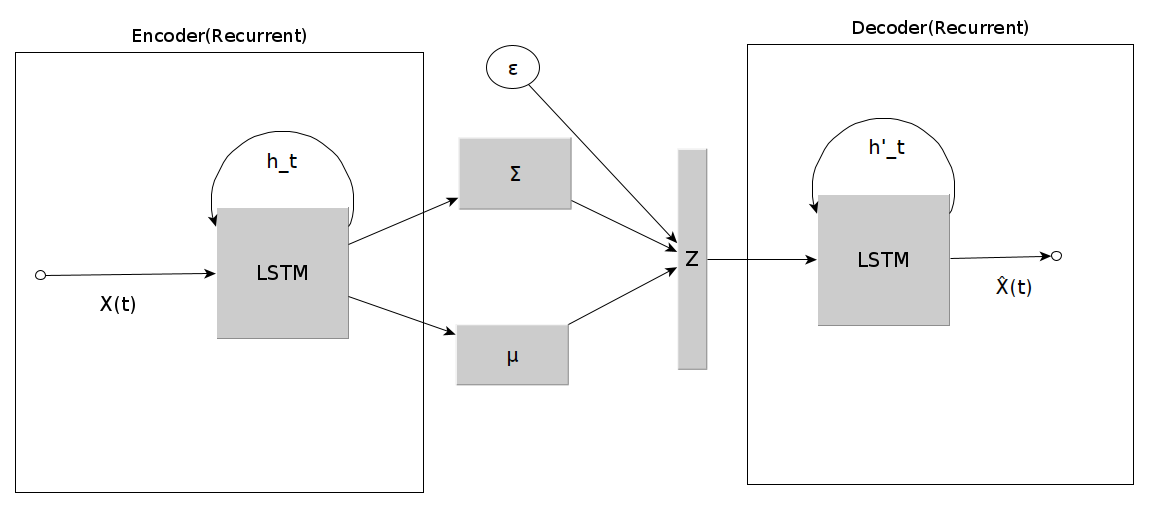
\includegraphics[scale=0.3]{architecture.png} 
%\begin{figure}
%\centering
%  \includegraphics[width=\linewidth]{figures/fig1.png}
% % archetecture.png: 1149x508 px, 72dpi, 40.53x17.92 cm, bb=0 0 1149 508
% \caption{Schematic diagram of RVAgene.}
% \label{fig:scheme}
%\end{figure}
%\end{center}


%% Probably too much detail here, but may want to cite the refs. 
%So far, we haven't specified anything about architecture of the encoder and decoder networks of a VAE, except that they learn certain functions modelling the posterior and likelihood probabilities  of our generative story of the data we are interested in. In general we could make them a fully connected neural network. But, since we are interested in handling sequential (time-series) data, we expect a specific structure of those functions. Intuitively, the $t$-th time point of input sequenece $\vx$ should be causally dependent only on its previous timepoints (upto $t-1$).  Therefore, instead of designing a completely agnostic network (e.g. fully connected layers), we can use a recurrent architecture for the encoder and decoder, which are well established in modelling sequence data (e.g. text data (\cite{Nallapati2016}), time-series data (\cite{Malhotra2015})). This in essence reduces the search space of the model from completely agnostic to a family of recurrent functions.
%\cite{Fabius2015} used this idea and showed how Recurrent Variational Autoencoders can be useful as a unsupervised latent representation learning and generative model for music data.


\subsection{RVAgene: A recurrent variational autoencoder to model gene expression dynamics}
Following the VAE architecture, RVAgene consists of an encoder and a decoder network with a reparameterization step in between. To incorporate the knowledge that we are modeling temporal data, recurrent neural networks offer an ideal architecture to use for both the encoder and the decoder networks. Recurrent and VAE networks have been successfully combined elsewhere, e.g. for textual \citep{Nallapati2016} and time series data \citep{Malhotra2015}.
\par
The architecture of RVAgene is based on \citet{Fabius2015}. An input sequence (i.e. gene) $x \in \vx$, $x = (x_1,x_2,...,x_t,...,x_T)$ is encoded using a recurrent function described by a long short-term memory (LSTM) unit. LSTM units are the state-of-the-art in recurrent architectures, since they are robust against the vanishing gradient problem for longer sequences, unlike other recurrent units (see details in \citet{Hochreiter1997}). We encode $x$ in the following manner:
\begin{align*}
 h_{t+1}^{enc} &= \textrm{LSTM}(W_{enc}^Th_t^{enc} + W_{inp}^T{x_t}+b_{enc}), \numberthis \label{lstm}
\end{align*}
where ($W_{enc}$, $W_{inp}$ and $b_{enc}$) are network weight parameters, and the hidden states $h_t$ represent information shared over timepoints in the LSTM. The dimension of the $h_t$ (and  $W_{enc}$) is given by a hyperparameter (``hidden-size''). The encoded $h_{t+1}$ are used to parametrize the posterior mean and variance from $x$, with mean $\mu_z$ and diagonal covariance $\sigma_z$ as:
%represent this mean and diagonal covariance matrix of the normal distribution an input $x$ is getting encoded to. 

\begin{align*}
 \mu_z &= W_{\mu}^Th_{T+1}^{enc} + b_{\mu} \numberthis \label{mu}\\
  log(\sigma_z) &= W_{\sigma}^Th_{T+1}^{enc} + b_{\sigma}.  \label{sigma}
 \end{align*}
We then use the reparameterization step described in \citet{Kingma2014} to sample $z$ from the distribution:
\begin{align*}
 z = \mu_z + \epsilon\sigma_z, \numberthis 
\end{align*}
where, for known $\epsilon$, backpropagation through the sampling step is possible while training the network.
\par
For the decoder network, the first state $h_1$ is calculated from $z$, and the recurrent formulation follows by reconstructing $x$ as $\hat{x} = (\hat{x}_1,\hat{x}_2,...,\hat{x}_t,...,\hat{x}_T )$, thus:
\begin{align*}
 h_1^{dec} &= \textrm{sigm}(W_{z}^Tz + b_{z})   \\
h_{t+1}^{dec} &= \textrm{LSTM}(W_{dec}^Th_t^{dec} + W_{out}^T{\hat{x}_t}+b_{dec}) \numberthis \label{decoder_lstm} \\
\hat{x}_t &= \textrm{sigm}(W_{out}^Th_t^{dec} + b_{out}), \\
\end{align*}
where $\textrm{sigm}(u) = \frac{1}{1 + e^{-u}}$ is the sigmoid activation function, and ($W_i, b_i$) are the network weight parameters. A schematic diagram of the network is shown in \hyperref[fig:fig2]{Fig. 1A}, which can now be trained using backpropagation, to minimize the objective function: 
\begin{align*}
    \cL(\theta, x) = D_{KL}(\cN(\mathbf{\mu}_z,\Sigma_z)||\cN(\mathbf{0},\vI)) + |x - \hat{x}|, \numberthis \label{lossfunction}
\end{align*}
where $\mathbf{\mu}_z$ and $\Sigma_z = \textrm{diag}(\sigma_z)$ are calculated from $x$ by the encoder.
\par 
To evaluate the accuracy of RVAgene, we need an appropriate error measure. For each gene in the test set, we calculate the $L1$ reconstruction error between generated data $\hat{x}$ and true data $x$, averaged over all time points. We normalize the data to lie in $[0,1]$ to avoid skewing the error by differences in gene expression magnitudes. Thus we define:
\begin{align}
    \textrm{Reconstruction error}(x,\hat{x}) = \frac{1}{T}\sum_{t}| s(\hat{x})_t - s(x)_t |,  & \text{ where } s(x) = \frac{x}{\sum_{t=1}^Tx_t}.
\end{align} 

\subsection{Generating synthetic gene expression time series data}
To test RVAgene, we generate a synthetic time series dataset. Six clusters each containing 20 genes are simulated, where for each cluster $c$, the mean gene expression time series $Y_c = (y_{c1}, y_{c2}, ..., y_{ct})$ was generated using addition or convolution and rescaling of two random sinusoidal functions of the form $k_1\textrm{sin}(k_2t)$, where $k_1,k_2$ are randomly chosen positive integers. Trajectories of cluster members were then generated by sampling from the multivariate normal $\cN(Y_c,\Sigma_c)$. We model $\Sigma_c$ as the positive definite matrix $\alpha Y_cY_c^T$, where $\alpha$ is a scaling factor, we use: $\alpha = 1/|Y_c Y_c^T|$. As defined, $\Sigma_c$ will describe nonzero correlations for all pairs of time points, $(t_i,t_j)$. This is unrealistic, so we set to 0 the entries of $\Sigma_c$ for which column and row indices have a difference of more than some threshold $T$ (we used $T=50$), reflecting the fact that correlations between time points are lost over larger time windows (temporal correlations are local). Note that under this condition, $\Sigma_c$  is no longer necessarily positive definite. The multivariate Gaussian sampler \verb+numpy.random.multivariate_normal()+ implemented in \verb+numpy+ \citep{harris2020array} was used to sample from this augmented $\Sigma_c$.
{After generating a simulated dataset by this process, we also added Gaussian noise, drawn from $\cN(0,0.7)$, to the simulated dataset to produce an additional dataset exhibiting higher levels of noise.}


%\section{Results} We compare binding site prediction results between two Geobind networks, one
without a CCRF layer (noCRF) and one with a CCRF layer as its second last layer (CRF). For both
cases we trained and validated the networks on three different datsets. The datasets used are as
follows:\\ \\ \textbf{PDNA-62 :} \citet{ahmad2004analysis} constructed a non-redundant dataset of 62
protein–DNA complexes which has been used in a variety of other studies
\citep{kuznetsov2006transient, wang2006bindn} etc. The protein sequences used were filtered to
ensure a maximum identity of no more than 25\% between any two sequences and the resolution of the
chosen structures was 2.5 A or better. The structures in this dataset contain only helical B-form
DNA.\\ \textbf{PDNA-74 :} We constructed a dataset of 74 single-stranded DNA binding proteins bound
to target ssDNA. We first used the structural database DNAproDB
\citep{sagendorf2017dnaprodb,sagendorf2020dnaprodb} to identify 374 protein-ssDNA complexes based on
structural critera which included ensuring the bound DNA in the structure presented the
single-stranded secondary structure, a minimum length of 4 nucleotides per DNA strand and 40
residues per protein chain, and a minimum of 5 nucleotide-residue interactions (as defined by
DNAproDB). Next, we verified that all proteins identified had known ssDNA binding function based on
annotations from the Gene Ontology knowledgebase \citep{gene2019gene}.  Finally, all protein
sequences were clustered with a 70\% sequence identity threshold using CD-HIT \citep{li2006cd}.
These clusters were then randomly sampled, with up to three samples per cluster, to generate the
final set of 74 protein structures. This sampling method allows us to construct a dataset with
limited amount of sequence redundancy but more conformational sampling than would be possible with a
stricter requirement on sequence redundancy. This is useful in the case of ssDNA where the polymer
is very flexible, but structural data is limited.\\ \textbf{PDNA-224:} a non-redundant dataset of
224 protein-DNA complexes originally constructed by \citet{li2013predna}\\ \begin{center}
        \begin{figure}
                \makebox[\textwidth]{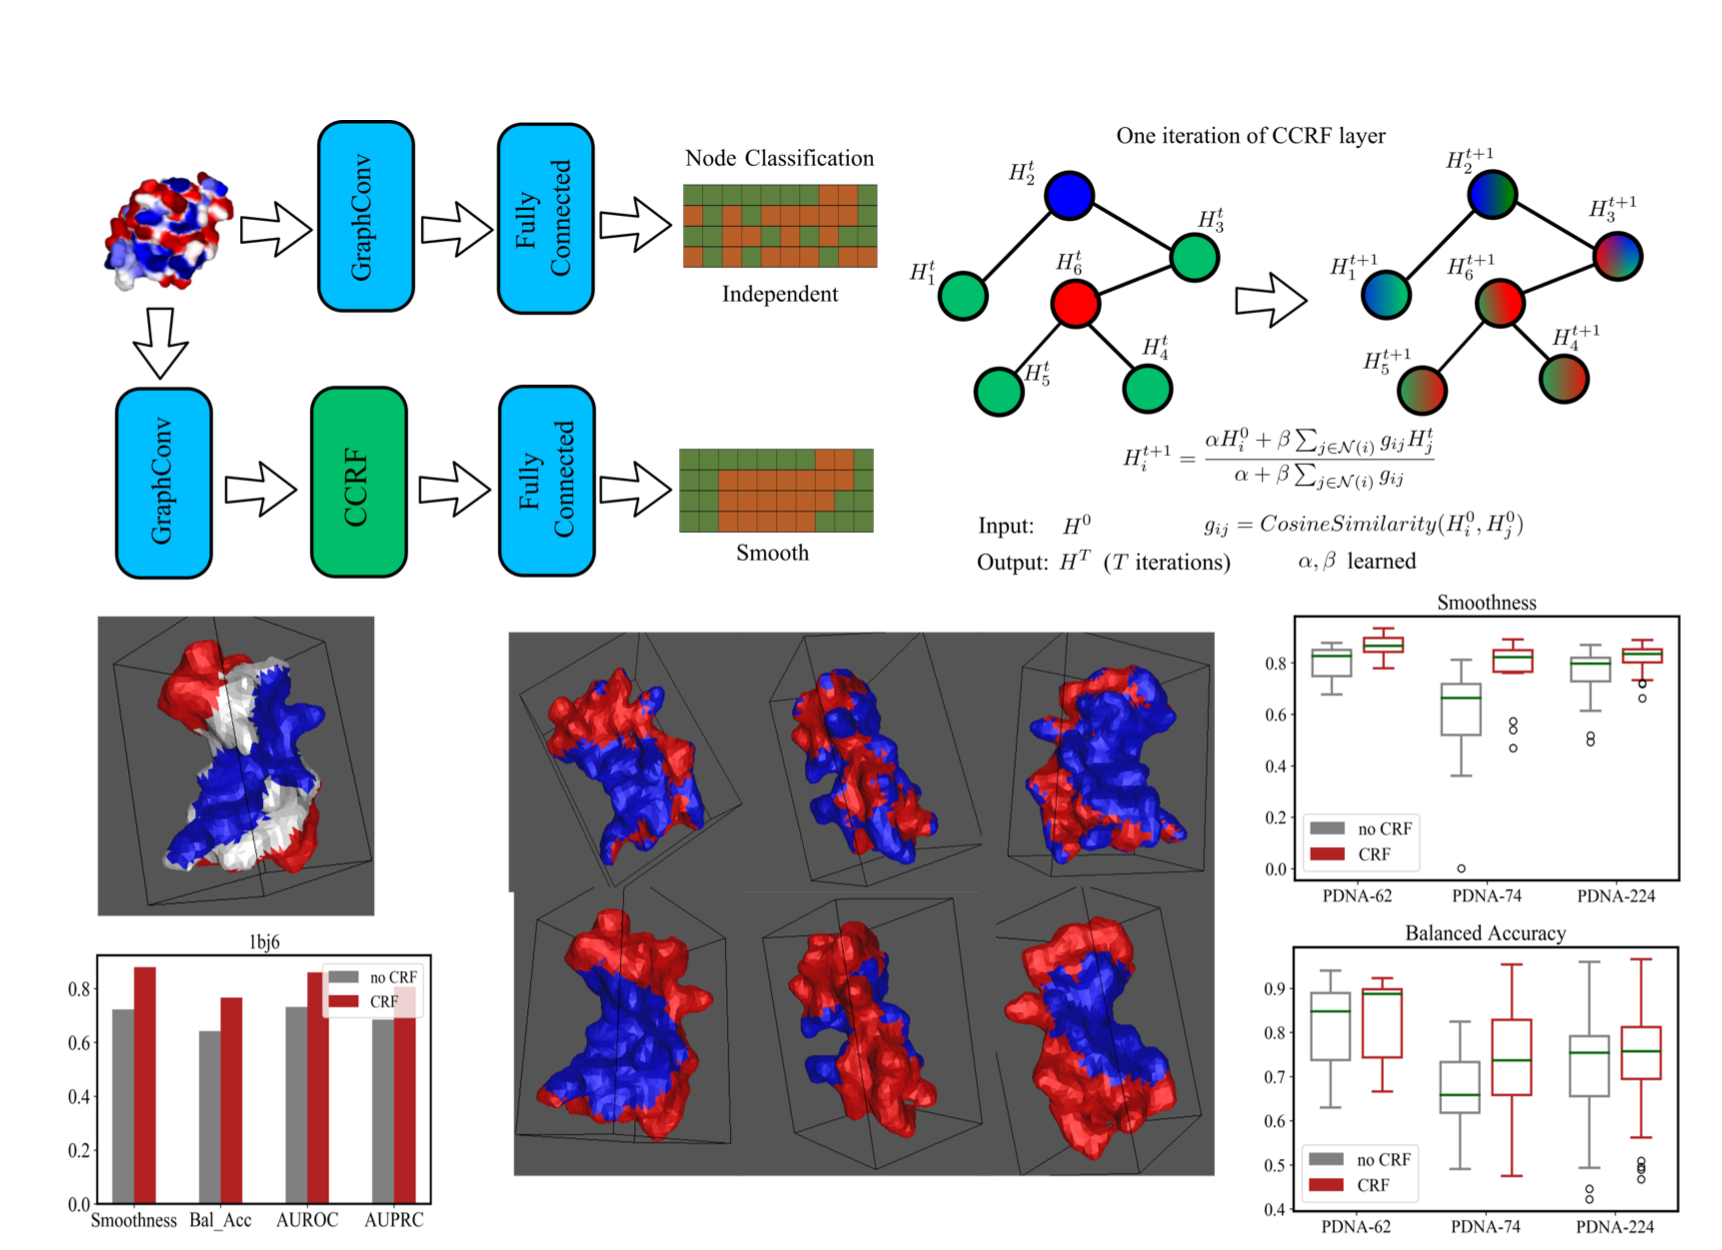
\includegraphics[width=0.8\paperwidth]{crf_figs/demo_crf_fig.png}}
 % archetecture.png: 1149x508 px, 72dpi, 40.53x17.92 cm, bb=0 0 1149 508
        \caption[CCRF for smooth binding site label prediction over protein surface.]{\textbf{CCRF
        for smooth binding site label prediction over protein surface.} ({\bf A}) ({\bf B}) }
        \label{fig:ccrf} \end{figure} \end{center}

Both CRF and noCRF models were trained on the three datasets with a 4:1 training and validation set
        split. \red{\hyperref[fig:ccrf]{Fig. 2.1D}} shows smoothness( eq.
        \ref{final_smoothness_metric}) and Balanced Accuracy  metrics achieved on the validation set
        in each case. We can clearly the smoothness of the predictions have increased significantly.
        It should also be noted that that, median Balanced Acuracy has also increased for all three
        cases. Therefore, we can conclude applying the CCRF layer improves the smoothness of the
        predicted labels over mesh vertices without compromizing in accuracy of prediction. For a
        more visual understanding, \red{\hyperref[fig:ccrf]{Fig. 2.1C}} shows one particular example
        of the effect of using CRF layer against the noCRF model for a protein in the validation set
        for PDNA-74 dataset. The top left panel in \red{\hyperref[fig:ccrf]{Fig. 2.1C}} shows the
        ground truth data. We can clearly see how the CRF model improves smoothness of the
        prediction along with various other classification metrics.



%\section{Discussion}
In this chapter we applied mean field Bayesian Variational inference to
design a network layer for PNAbind which results in smoother binding site predictions on protein surfaces. We also designed a smoothness metric appropriate for the task of protein surface segmentation.

In the PNAbind framework, the model predicts whether a protein would bind nucleic acids or not, and segments the protein surface into binding and non-binding regions. However, it does not try to predict binding specificity (i.e. what nucleic acid sequence is preferred) and is only based on protein surface and physicochemical features. We assume there are some commonalities between the proteins binding to, say, ss-DNA (for PDNA-74) and this model implicitly learns those sets of commonalities. 

The PNAbind package has been published as joint work led by Jared Sagendorf, who mentored me in this project, with contributions from Jiawei Hunag, Prof. Xiaojiang Chen and supervised by Prof. Remo Rohs\citep{Sagendorf2024}. In recent years multiple works have been published which compete with PNAbind \citep{gainza2020deciphering, gligorijevic2021structure, yuan2022alphafold2, xia2021graphbind, tubiana2022scannet, krapp2023pesto, li2023geobind, sverrisson2021fast}. But, no deep learning method to predict binding specificity across protein families has been achieved yet.

As a next step, we work towards predicting binding specificity. One of the key challenges in this problem setting is data sparsity. In the next chapter, we present DeepPBS, a model for protein-DNA binding specificity prediction, based on a given co-crystal structural model, which works across protein families.  


%%%%%%%%%%%%%%%%%%%%%%%%%%%%%%%%%%%%%%%%%%%%%%%%%%%%%%%%%%%%%%%%%%%%%%%%%%%%%%%
%\chapter{Proposal:  A generalized generative model for binding element design.}
%\begin{abstract} 
    Predicting DNA/RNA binding sites on a given protein surface is an important computational task since experminetally determining such information is often expensive and time consuming. Such binding site prediction task can be formulated as a node classification task over a 3D mesh representing the protein surface, with features over the vertices and edges of the mesh representing various geometrical and physicochemical features of the protein structure. At our lab we developed a deep learning based method, which independently classifies mesh vertices as binding and non-binding sites. This often results into irregular binding site predictions over the protein surface. However, intuitively, binding site predictions should be contiguous and not patchy i.e. as ``smooth" as possible while being correct. In this chapter, we describe what such kind of ``smoothness" entails and we improve upon the original architecture by desigining a network layer based on a  probabilistic Continuous Conditional Random Field (CCRF) model, which increases smoothness of binding site prediction while improving prediction accuracy of the model. This network layer was incorporated into the original model and published as Geobind package (\red{Sagendorf et. al}).
\end{abstract}

%\section{Introduction} 

Designing binding elements for target regions in protein residues or complexes is a hard
computational problem  which has huge impact in biotechnology and pharmaceutical ventures.
This constitutes of drug design and nucleic acid sequence/position weight matrix (PWM)
design. The processes generally employed in solving these kind of problems are traditionally virtual and
experimental screening of large amount of candidate binding elements. These processes are extremely
computationally/experimentally intensive and costly. 
\par
Recently, generative machine learning models have
been used to make significant advances in such tasks. The key models generative models that are most
used are mainly of two kind: Variational Autoencoders (VAE) \citep{Kingma2014} and its many
variations \citep{higgins2016beta, sohn2015learning,dilokthanakul2016deep}; Generative Adversarial
Networks \citep{goodfellow2014generative} and variations \citep{wang2018high,zhu2017unpaired}.
\citet{gomez2018automatic} first proposed a variational autoencoder model for drug molecule design.
Similar to RVAgene \red{(cite)} this method encodes training drug molecules represented as SMILES
\citep{weininger1988smiles} string in a regularized latent space which then can be sampled and
decoded to generate new candidate molecules. They also train an additional network to optimize the
generative process based on given chemical properties. This initial model sparked a flurry of folow up 
works mainly addressing various aspects of the problem: e.g. enforcing constraints on the generative process 
such that the generated molecules are chemically valid \citet{kusner2017grammar}, increasing diversity of the generated
molecules, conditional generation etc. 

%\section{Proposed Method} 
In chapter 1, we learned a generative model of gene expression time
series data using a VAE framework, where we learned a regularized latent space representation of latent
variables $z$ by reconstructing the data $x$ through an encoder-decoder architecture. We can start
thinking about the binding element design problem in the same manner.

Let's define $x_p$ as input binding site information. We want to predict a binding element $x_e$
given $x_p$. To achieve this task, we again formulate a generative story: $x_e$ is generated from
latent variables $z$, which can be modeled by a decoder/generator network which models the
distribution $P(x_e|z)$. And we can employ an encoder network modeling $P(z|x_p)$ to achieve the
latent information $z$ from the input $x_e$.

Now, to formally achieve the prediction task, we start with writing out the conditional distribution,
$P(x_e, z|x_p)$ which we would like to maximize and predicts the argument $x_e$ and $z$ that maximizes it.

\begin{align*}
        P(x_e,z|x_p) = P(x_e|z,x_p)P(z|x_p) \;\;\; \text{using Bayes' rule}\numberthis
\end{align*}
Here, we assume a hierarchical Bayesian setting where given the latent variable $z$, $x_e$ is
generated independent of $x_p$ i.e. $P(x_e|z,x_p) = P(x_e|z)$. Now we can write the following,
\begin{align*}
P(x_e,z|x_p) &= P(x_e|z)P(z|x_p) \numberthis \\
\end{align*}
Now, we can model the posterior of $z$, $P(z | x_p)$ as a Gaussian $N(z_{\mu}, z_{\Sigma})$. This
can be modeled by outputing the parameters $z_{\mu}, z_{\Sigma}$ from an encoder network $E(x_p)$.
A value of $z$ can be sampled from this distribution now using the reparamtrization trick described
in \citet{Kingma2014}, similar to as described in Chapter 1 for RVAgene. This process along with a
KL loss with a prior on $z$ $p(z) = N(0,\bI)$ ensures a regularized latent space which is important
for generating meaningful data. Therefore,
\begin{align*}
        z_{\mu}, z_{\Sigma} &= E(x_p) \numberthis \\
        \hat{z} &= z_{\mu} + \epsilon \cdot z_{\Sigma} \;\; where \;\; \epsilon \sim N(0,\bI) \numberthis \\
        \hat{x}_e &= argmax_{x_e}p(x_e | \hat{z}) = G(\hat{z}) \;\; \numberthis \label{final_prediction_architecture} 
\end{align*}
%\implies \text{prediction } \hat{x}_e, \hat{z} &= argmax_{x_e,z} P(x_e,z|x_p) \numberthis \\
%&= argmax_{x_e,z} P(x_e|z)P(z|x_p)  \\
%\implies  \hat{z} = argmax_{z} P(z|x_p); & \;\;\;\;\hat{x}_e = argmax_{x_e} P(x_e | \hat{z}) \numberthis \\
%\implies \hat{z} = E(x_p); & \;\;\;\; \hat{x}_e = G(\hat{z}) \numberthis
The functions $E(x_p)$ and $G(\hat{z})$ in \ref{final_prediction_architecture} represent the
encoder and generator functions respectively both of which are parametrized by neural networks. 

Now, the encoder-generator framework described above is suitable for prediction, however it's
difficult to train it in a straight forward manner. For RVAgene \red{(cite)} we were able to use
reconstruction based method to train because the input of encoder and output of decoder was the same.
Here, they are different. This constitutes a proper scenario to employ an adversarial training
scheme as employed by GANs \citep{goodfellow2014generative}.

Given a training dataset $X$ consisting of $n$ datapoints, where $X_i = (x_p^i, x_e^i) \;\; i \in
\{0,..., n-1\}$, we now describe
how to train the generative model described in \ref{final_prediction_architecture}. We assign a
label variable $y = 1$ for all datatpoints in the training data $X$. Now, assume we have some
datapairs $F = (x_p^i, \hat{x}_e^i) \;\; i \in \{0,..., m-1\}$ generated by the encoder-generator
system given $x_p^i$s as input. We assign these datapoints a label $y = 0$. Now, we can train a
neural network $D$ discriminating between the datasets X and F i.e. the discriminator $D$ is
predicting $P(y = 1 | x_p, x_e)$. It is clear that the better the enocder-generator system is in
predicting binding element given a protein surface, the harder the job of the discriminator becomes.
We take advantage of this fact and teach the encoder-generator network to try to best the
discriminator and vice versa. The two networks play the following minimax game:
\begin{align*}
        min_{G,E}max_{D} V(D, E, G) &= \bE_{x_p, x_e \sim P_X}\bigg{[}log D(x_p, x_e)\bigg{]} + \bE_{x_p \sim
        P_{x_p}}\bigg{[}log(1 - D(x_p,G(\hat{z}))) + KL(N(z_{\mu}, z_{\Sigma}) || N(0, \bI))\bigg{]} \numberthis \label{gan_game}\\
        &where \; \hat{z} = z_{\mu} + \epsilon z_{\Sigma} \;\; where \; \epsilon \sim N(0,\bI)\; and \;
        z_{\mu}, z_{\sigma} = E(x_p)
\end{align*}
In eq. \ref{gan_game} above $P_X$ represents the full training data distribution and $P_{x_p}$
represents the marginal distribution of binding sites in the training data. 

If we call the generated distribution of $x_p, \hat{x}_e$ as $p_g$, as described and proven in
\citet{goodfellow2014generative} this adversarial game 
eventually results into the generated data distribution becoming same as the training data
distribution $P_x$, which
happens at the point when both the $(E, G)$ and $D$ network cannot improve anymore.

%\section{Discussion}
In this chapter we described our proposal for designing a generative model for design binding
elements given binding site information on protein surface. The proposed model is a variation over the VAE
framework \citep{Kingma2014} for unsupervised representation learning. However, it should be noted,
that the architecture described here is not final can change after further experimentation.

Next, we need to shade a little bit of light on the datasets that can be used to train such a model.
Primary source for all our data will be the protein data bank \citep{berman2000protein}. For PWM
generation, the databases JASPAR \citep{fornes2020jaspar} and TRANSFAC \citep{wingender2008transfac}
are good candidates for sources of protein-motif data. However, it should
be noted that, for nucleic acid PWM generation, although the prediction task is PWM generation, the
training data does not need PWM information. Computationally sequences and PWMs are equevalent. the model
sees both sequences and PWMs as a vector of dimension $L \times 4$ ($L$ is length of the
sequence/PWM). Only difference, the vectors are one-hot for sequence and can have fractional values
for PWMs i.e PWMs are soft sequences only. Therefore, it is possible to train the model with
sequence data directly provided the data is rich enough and PWM information is not needed in the
training set. 

Another point that should be discussed is concerning the architecture of Encoder and Generator
networks. The encoder network, although performing the same task for both the drug molecule
generation setting and PWM generation setting, may need to have different architectures. This may be necessary because binding sites for drug molecules are much smaller tha
nucleic acid binding sites (which therefore, can also be discontinuous). This would lead to a point
cloud representation being more favourable compared to mesh representation for PWM generation task.
The generator network will have different architectures based upon the way the binding element
generated is represented as discussed earlier in this chapter.

We hope this project becomes a success and we can present it as a powerful computational tool to the
Computational Biology and Bioinformatics community.


%%%%%%%%%%%%%%%%%%%%%%%%%%%%%%%%%%%%%%%%%%%%%%%%%%%%%%%%%%%%%%%%%%%%%%%%%%%%%%%%%%%%%%%%%%%%%%%%%%%%%%%%%%%%%%%%%%%%%%%%%%%%%%%%%
\chapter{Geometric deep learning of protein–DNA binding specificity}
%\begin{abstract}
Structure based study and mechanistic prediction of protein-DNA binding specificity is a key interest in the
current state of structural biology. In particular, analyzing protein-DNA co-crystals from PDB has
        become a staple in everyday structural biology. However, we still do not have co-crystals
        for a particular protein bound to a varied set of DNA structures. On the other hand, these variations in
        DNA-binding are available from experimental data. These experiments do not easily give
        insight into binding mechanism and are expensive to perform. Hence, a valuable question worth
        asking is given one protein-DNA co-crystal can one predict the full range of DNA binding
        specificity for the protein in the co-crystal in question.

        In fact, the space of dna-binding proteins and corresponding binding mechanism is extremely
        varied. Local chemical interactions as well as energetics of the global shape of
        protein and DNA in context of binding determine these specificities. Current availability of structural
        data, although not abundant but suffices to model this complicated problem via deep
        learning. In this work we build a modular deep learning model which can generalize and learn from
        various aspects of a given co-crystal and produces binding specificity prediction.
\end{abstract}

%\section{Introduction} 

Transcription factors play critical roles in various regulatory functions that are essential to all aspects of life \citep{Spitz2012}. Therefore, understanding the mechanisms by which proteins target specific DNA sequences is crucial \citep{Zhao2009}. Extensive research has uncovered myriad binding mechanisms that lead to specific high-affinity binding, including strong electrostatic interaction of arginine residues in the DNA minor groove \citep{rohs2009role}, deoxyribose sugar-phenylalanine stacking \citep{stirnimann2010structural}, bidentate hydrogen bonds (H-bonds) between guanine (G) and arginine (Arg) in the major groove \citep{Helene1977}, and other interactions \citep{Rohs2010,Schildbach1999,Seeman1976}.
\par
Protein-DNA structures are typically \citep{Garvie2001} obtained through X-ray crystallography, nuclear magnetic resonance spectroscopy or cryo-electron microscopy experiments and stored in the Protein Data Bank (PDB) \citep{berman2000protein}. Generally, these structures display one bound DNA sequence and the associated physicochemical interactions6 but do not encompass the full range of potentially bound DNA sequences. Conversely, this information can be experimentally obtained through protein-binding microarray \citep{Berger2009}, systematic evolution of ligands by exponential enrichment combined with high-throughput sequencing (SELEX-seq) \citep{Slattery2011}, chromatin immunoprecipitation followed by sequencing \citep{Park2009}, high-throughput SELEX \citep{Jolma2013} or related high-throughput approaches \citep{Slattery2014}. These experiments capture the range of possible bound DNA sequences but do not necessarily provide structural information. In essence, these sets of experiments are complementary, and manual examination is often required to correlate molecular interaction details from structural data with binding specificity data \citep{rohs2009role}.
\par
Predicting binding specificity for a given protein sequence, across protein families, remains a challenging and unsolved problem, despite progress for specific protein families \citep{persikov2014novo, Wetzel2022, persikov2009predicting, Sofia2022, Meseguer2020, molparia2010zif, christensen2012recognition, Yanover2011}. Structural changes in the context of binding, along with large mechanistic diversity, contribute to the difficulty \citep{Slattery2014, Chiu2023}. Protein-DNA structures contain valuable information, which has been used to come up with models of specificity tested on small datasets \citep{morozov2005protein}. Artificial intelligence can leverage this information to broadly achieve generalizability across protein families. In this framework, we introduce Deep Predictor of Binding Specificity (DeepPBS). This deep-learning model is designed to capture the physicochemical and geometric contexts of protein-DNA interactions to predict binding specificity, represented as a position weight matrix (PWM) \citep{Stormo2013} based on a given protein-DNA structure (Fig. 1a). DeepPBS functions across protein families (Fig. 2) and acts as a bridge between structure-determining and binding specificity-determining experiments. 
\par
Input of DeepPBS is not limited to experimental structures (Fig. 1a). The rapid advancement of protein structure prediction methods, including AlphaFold \citep{Jumper2021}, OpenFold \citep{Ahdritz2024} and RoseTTAFold \citep{Baek2021}, along with protein-DNA complex modelers, such as RoseTTAFoldNA (RFNA) \citep{baek2024na}, RoseTTAFold All-Atom \citep{Krishna2024}, MELD-DNA \citep{Esmaeeli2023} and AlphaFold3 \citep{Abramson2024}, have led to an exponential increase in the availability of structural data for analysis. This scenario highlights the growing need for a generalized computational model to analyze protein-DNA structures. We demonstrate how DeepPBS can work in conjunction with structure prediction methods for predicting specificity for proteins without available experimental structures (Fig. 3a-d). In addition, the design of a protein-DNA complex can be improved by optimizing bound DNA using DeepPBS feedback (Fig. 3e-g). We show that this pipeline is competitive with the recent family-specific model rCLAMPS \citep{Wetzel2022} (Fig. 3h,i) while being more generalizable: specifically, DeepPBS is protein family-agnostic, can handle biological assemblies and can predict DNA flanking preferences.
\par
In terms of interpretability, ‘relative importance’ (RI) scores for different heavy atoms in proteins that are involved in interactions with DNA can be extracted from DeepPBS (Fig. 4). As a case study on an important protein for cancer development, we analyze the p53-DNA interface via these RI scores and relate them with existing literature for validation. Additionally, we show that the DeepPBS scores align well with existing knowledge and can be aggregated to produce reasonable agreement with alanine scanning mutagenesis experiments \citep{Morrison2001} (Fig. 4h).
\par
In additional proof-of-principle studies, we apply DeepPBS to in silico-designed protein-DNA complexes targeting specific DNA sequences (Fig. 5), obtained from a recent study that combines structural design with DNA mutagenesis experiments \citep{Glasscock2023}. Finally, we show that DeepPBS can also be used to analyze molecular simulation trajectories. We demonstrate an example by applying DeepPBS to a molecular dynamics (MD) simulation of Extradenticle (Exd) and Sex combs reduced (Scr) Hox heterodimer in complex with DNA \citep{Joshi2007} with an AlphaFold-based modeled protein linker (Supplementary Section 10, Supplementary Fig. 6 ). DeepPBS is available as a webserver at https://deeppbs.usc.edu.
\par

\section{Results}
\subsection{The DeepPBS Framework}
The DeepPBS framework is illustrated in Fig. 1. Input to DeepPBS (Fig. 1a) is composed of one protein-DNA complex structure, with one or more protein chains bound to a DNA double helix. Potential sources for such structures include experimental data (for example, PDB\citep{berman2000protein}), molecular simulation snapshots or designed complexes. DeepPBS processes the structure as a bipartite graph with distinct spatial graph representations for protein and DNA components. The protein graph is an atom-based graph, with heavy atoms as vertices. Several features are computed on these vertices (Fig. 1b). Further information on protein representation and feature computation is available in Methods. We represent DNA as a symmetrized helix (sym-helix), as detailed in Methods. This representation removes any sequence identity that the DNA possesses, while preserving the shape of the double helix \citep{rohs2009role}. Optionally, DNA sequence information can be reintroduced as a feature on the sym-helix points.
\par
DeepPBS performs a series of spatial graph convolutions on the protein graph to aggregate atomic neighborhood information (Fig. 1d). The next crucial component of DeepPBS consists of a set of bipartite geometric convolutions applied from the protein graph to the sym-helix (Fig. 1d). Specific chemical interactions (for example, hydrogen bonds) depend on both location and orientation \citep{Helene1977}. DeepPBS learns how the geometric orientation of the sym-helix points is associated with the orientations and chemistry of neighboring protein residues. Four distinct bipartite convolutions are employed for the sym-helix points, corresponding to the major groove, the minor groove and the phosphate and sugar moieties. Major and minor groove convolutions are referred to as ‘groove readout’. This term was chosen over the term ‘base readout’ due to the removal of base identity in the sym-helix. Phosphate and sugar moiety convolutions, combined with DNA shape information, form the ‘shape readout’ (Fig. 1e). The ‘groove readout’ and ‘shape readout’ factors collaboratively determine binding specificity to varying extents for different protein families. At this point, the sym-helix representation enables a straightforward flattening of aggregated features on the three-dimensional sym-helix to the one-dimensional (1D) base pair-level features. By adding DNA shape information and implementing 1D convolutional neural network and prediction layers (Fig. 1e), DeepPBS ultimately predicts binding specificity (Fig. 1f). Further architectural details are described in Supplementary Section 5.
\par
Lack of an existing published standard dataset for predicting binding specificity across protein families from protein-DNA complex structure data made it necessary for us to build a dataset for cross-validation and benchmarking. Details of this process can be found in Methods.

\begin{center}
    \begin{figure}
    \makebox[\textwidth]{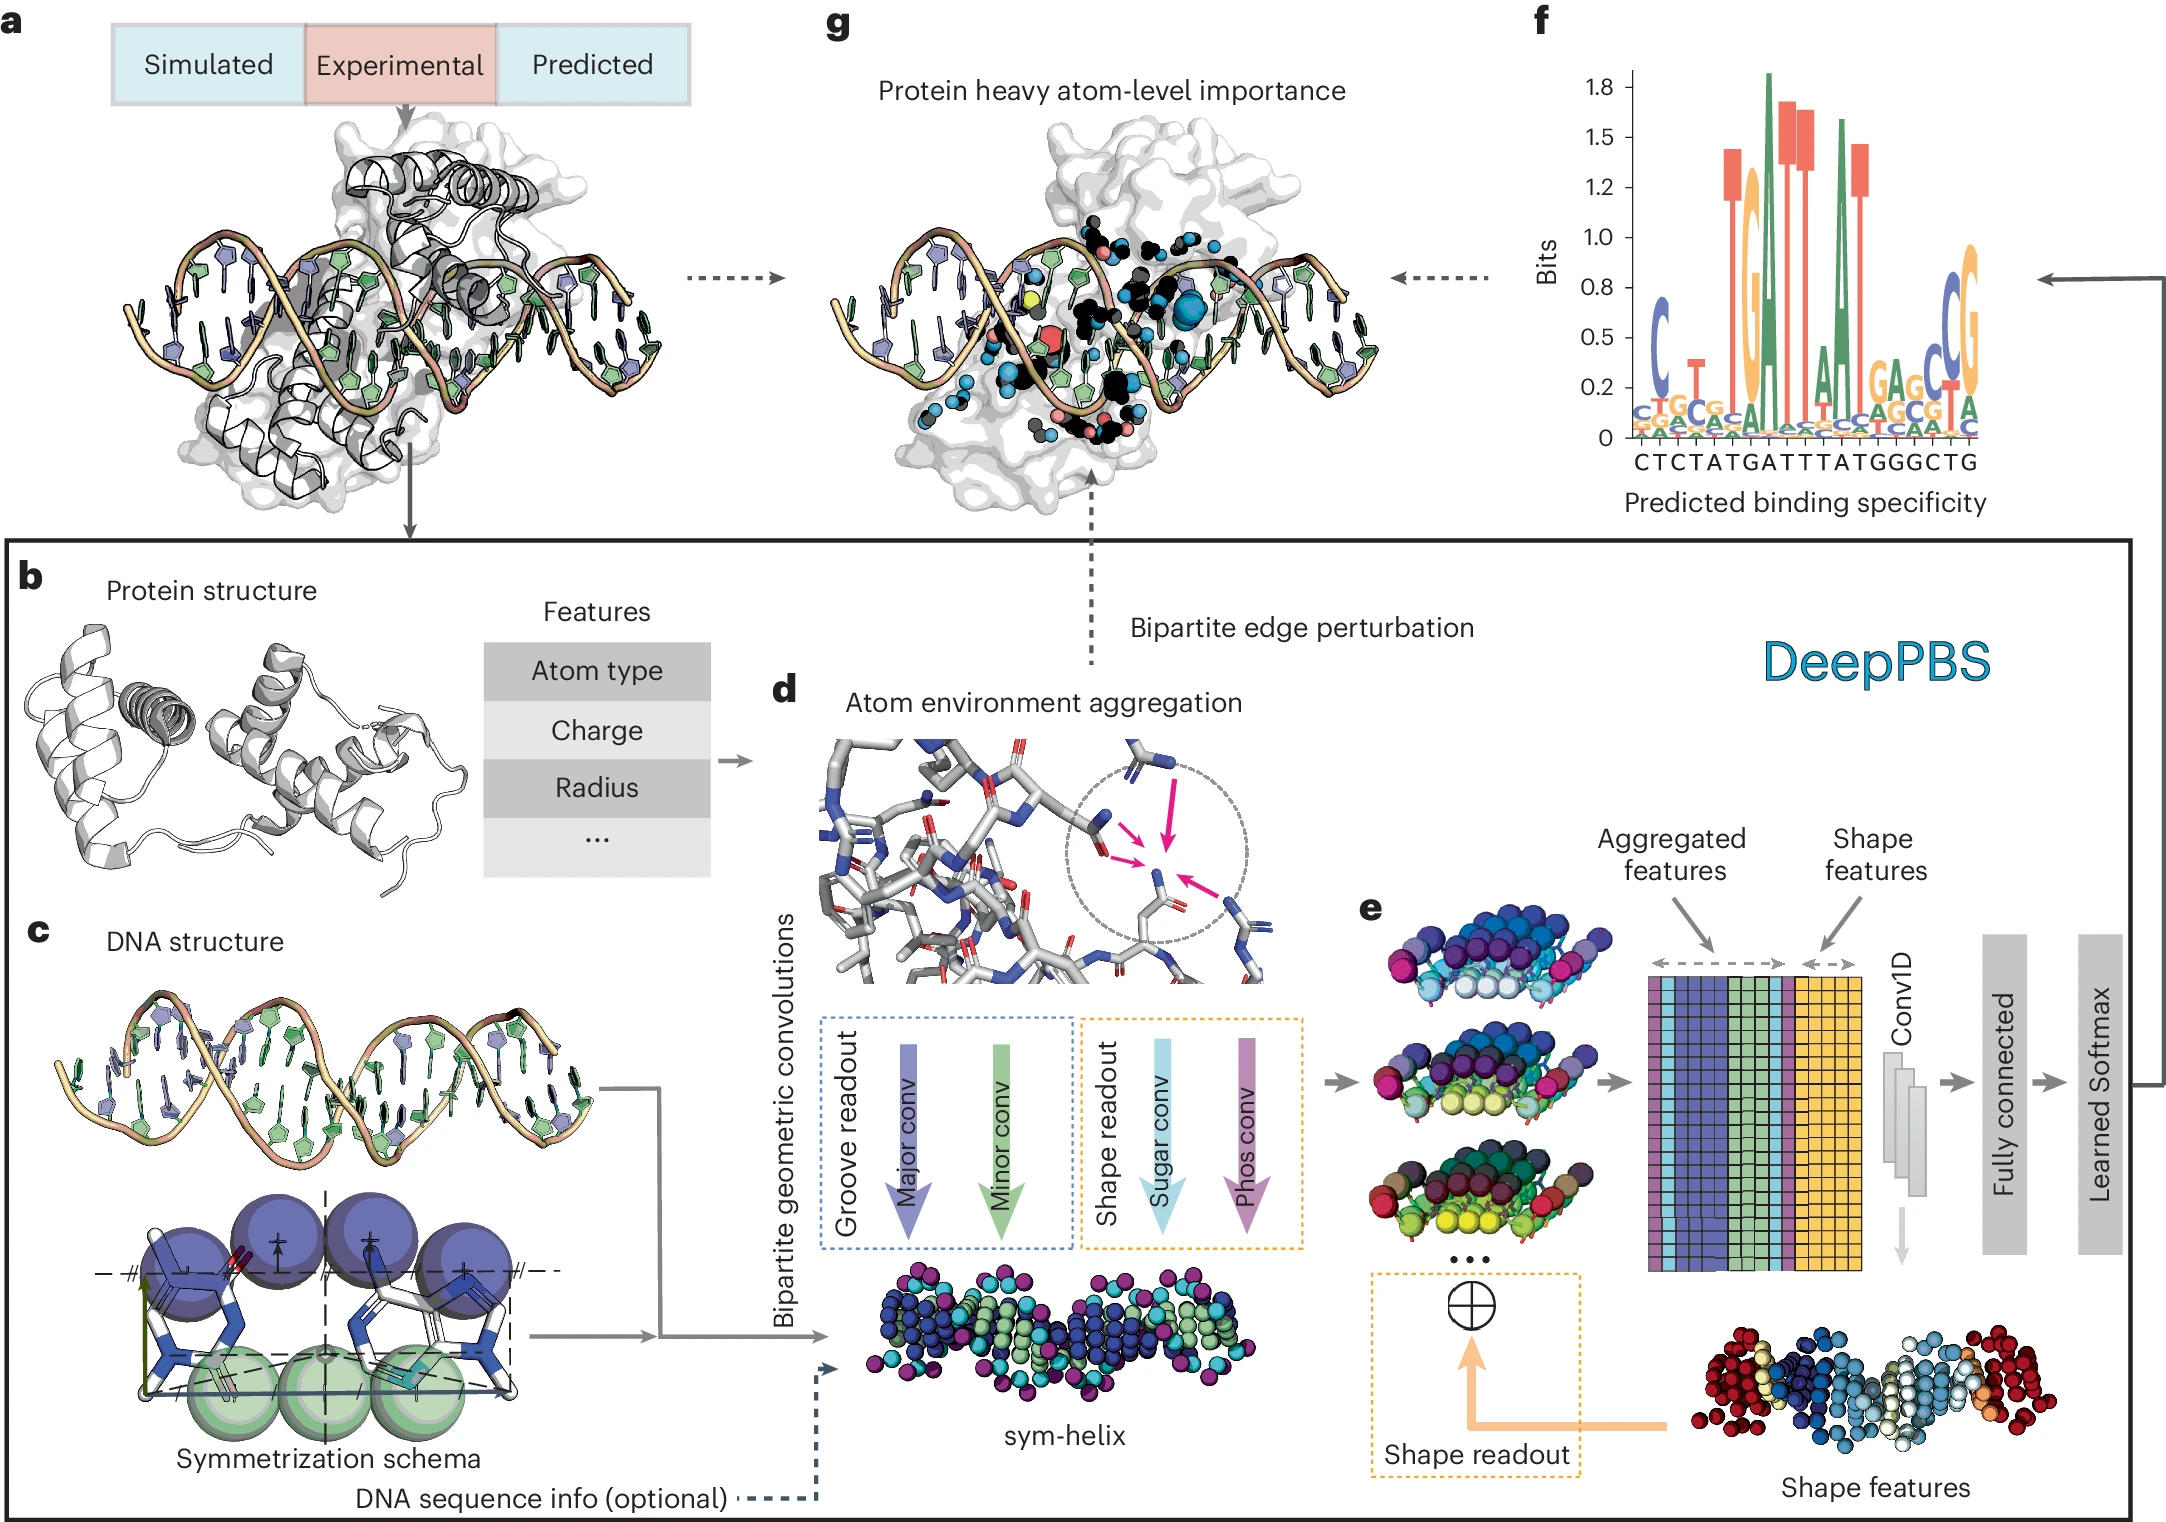
\includegraphics[width=0.8\paperwidth]{./pdnafigs/fig1.png}}
 % archetecture.png: 1149x508 px, 72dpi, 40.53x17.92 cm, bb=0 0 1149 508
        \caption[Computational cost of training RVAgene]{\textbf{Training RVAgene is reasonably scalable on CPU and even more so using hardware acceleration through GPU.} ({\bf A}) Time cost of training RVAgene for 100 epochs for datasets with varying number of genes and time points on CPU and GPU. ({\bf B}) Maximum memory utilized during training of the model on CPU an GPU for the cases in (A), inset plot: comparison of max memory used compared to DPGP for varying number of genes.}
  \label{fig:pdna1}
\end{figure}
\end{center}

\subsection{DeepPBS performance for experimentally determined structures}
The DeepPBS ensemble (Methods) was employed to evaluate model performance against a benchmark set, as outlined in Supplementary Section 1. The DeepPBS architecture allows models to be trained on two mechanisms: ‘groove readout’, which does not involve backbone convolutions and excludes shape information, and ‘shape readout’, which does not involve groove convolutions (Fig. 1d,e). Benchmark performances of DeepPBS (which performs both ‘groove readout’ and ‘shape readout’ modes combined) and these two variations are shown in Fig. 2a. The ‘groove readout’ version does better than the ‘shape readout’ version in terms of median performance, while the DeepPBS model improves upon either component in isolation (two-sided t-test P value <0.01; Fig. 2a). Pairwise t-test P values for these variations are available (Supplementary Data 1). A discussion of the outliers in Fig. 2a is provided in Supplementary Section 12.
\par
The dataset was constructed using experimentally determined structures; thus, the co-crystal structure-derived DNA sequence typically serves as a reasonable example of a bound sequence. As expected, integrating sequence information into the sym-helix points (‘DeepPBS with DNA SeqInfo’) enhanced performance (Fig. 2a), significantly closing the gap toward the inherent performance limit in the dataset. The inherent performance limit originates from the fact that for the same protein the binding specificity data presented by two databases \citep{Jaime2022, kulakovskiy2018hocomoco} used to create the dataset may disagree to some extent (Supplementary Fig. 1c). We computed the distribution of disagreement across all unique PWMs appearing in both databases (Supplementary Section 1). However, from both interpretability and design perspectives, particularly when the bound DNA sequence may not be representative, the ‘DeepPBS’ model is optimal due to its low sensitivity to the DNA sequence in the structure. This fact is evidenced by comparing performances of the ‘DeepPBS’ and ‘DeepPBS with DNA SeqInfo’ models in the context of the PWM-co-crystal-derived DNA alignment score (Supplementary Section 1). Compared with the line fit to the variation with DNA sequence information (slope $-0.44$ for root mean squared error (RMSE), slope $-0.62$ for mean absolute error (MAE); Supplementary Fig. 11), the slope of the line fit to the DeepPBS predictions was closer to zero (Fig. 2b and Supplementary Fig. 11).
\par
As an example, we show the DeepPBS ensemble prediction for the NF-$\kappa$B biological assembly from the benchmark dataset. Although the co-crystal structure-derived DNA sequence was not of the highest binding affinity, as indicated by experimental data from HOCOMOCO \citep{kulakovskiy2018hocomoco}, our prediction circumvented this issue, predicting a binding specificity that was more closely aligned with the experimental data (Supplementary Fig. 5d). Similar trends (Supplementary Fig. 5a-c) can be observed from cross-validation predictions by individual DeepPBS models (Methods). We also included example DeepPBS ensemble predictions (Supplementary Fig. 7) for structures in the PDB that correspond to specific interactions but do not have a PWM in the two binding specificity databases considered (Methods). In addition, example DeepPBS ensemble predictions (Supplementary Fig. 8) for structures of nonspecific protein-DNA binding (for example, SSO7D-DNA interaction \citep{Agback1998}) present in the PDB are presented. These predictions have notably lower information content compared with those in Supplementary Fig. 7.

\subsection{DeepPBS captures patterns of family-specific binding modes}
Abundances of different protein families in the benchmark set are described in Fig. 2c (Supplementary Fig. 5b for cross-validation set). Family annotations were obtained from the Database of Protein Families (PFAM) \citep{Mistry2021}. The dataset encompasses a wide range of DNA-binding protein families. Performance of DeepPBS for various protein families provides several key insights. DeepPBS showed reasonable generalizability across protein families, performing well even for families with relatively fewer structures (Fig. 2d and Supplementary Fig. 5c), such as heat shock factor proteins. This observation suggests that the model is learning the underlying mechanisms of protein-DNA binding rather than overfitting on family-specific patterns.
\par
Further validation is provided by comparing performances of the DeepPBS ‘groove readout’ and ‘shape readout’ models (Fig. 2d and Supplementary Fig. 5c). For families like zf-C2H2, zf-C4 the ‘shape readout’ model did not perform as well as the ‘groove readout’ model. This result aligns with the common understanding of the binding mechanism of these families. For example, zf-C2H2 uses zinc finger motifs to scan DNA for suitable base interactions, with minimal DNA bending or conformational change \citep{Persikov2011}. This binding mode makes the zf-C2H2 family a popular target of protein sequence-based binding specificity prediction and design \citep{Persikov2014, persikov2009predicting, aizenshtein2022deepzf, Yanover2011, Ichikawa2023}. Conversely, families like interferon-regulatory factor (IRF) proteins (Fig. 2d and Supplementary Fig. 5c) and T-box proteins (Supplementary Fig. 5c) showed higher performances for the ‘shape readout’ model, consistent with their known binding mechanisms that involve significant conformational changes\citep{Stirnimann2010, Escalante1998}. For families such as homeodomain (HD) and forkhead (Fig. 2d and Supplementary Fig. 5c), the DeepPBS model outperformed both the ‘groove readout’ and ‘shape readout’ components. This result suggests that the network captures complex higher-order relationships of these components. Pairwise P values for the three readout variations for Fig. 2d and Supplementary Fig. 5c are available in Supplementary Data 1.

\begin{center}
    \begin{figure}
    \makebox[\textwidth]{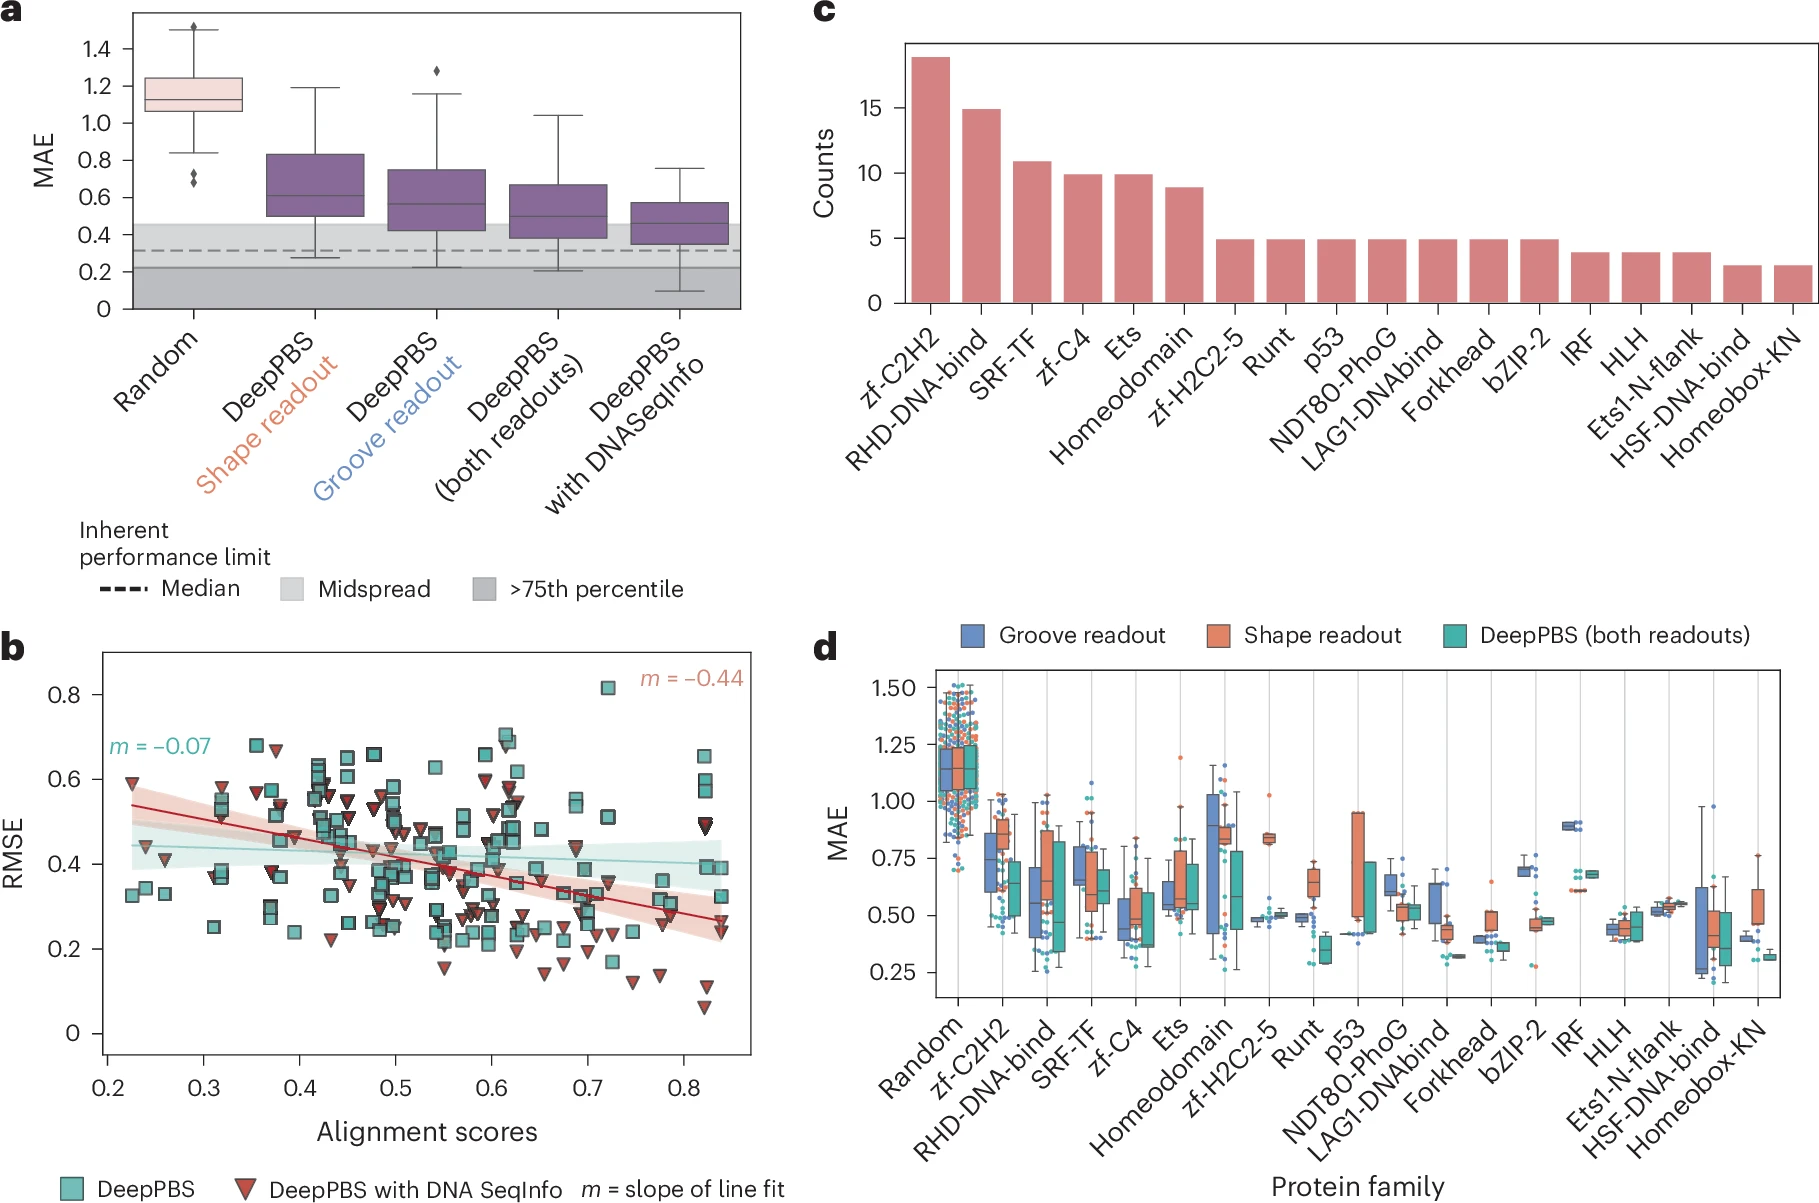
\includegraphics[width=0.8\paperwidth]{./pdnafigs/fig2.png}}
 % archetecture.png: 1149x508 px, 72dpi, 40.53x17.92 cm, bb=0 0 1149 508
        \caption[Computational cost of training RVAgene]{\textbf{Training RVAgene is reasonably scalable on CPU and even more so using hardware acceleration through GPU.} ({\bf A}) Time cost of training RVAgene for 100 epochs for datasets with varying number of genes and time points on CPU and GPU. ({\bf B}) Maximum memory utilized during training of the model on CPU an GPU for the cases in (A), inset plot: comparison of max memory used compared to DPGP for varying number of genes.}
  \label{fig:pdna2}
\end{figure}
\end{center}

\subsection{Application to in silico-predicted protein–DNA complexes}
The DeepPBS framework is not limited to experimental structures. Recent advances in scalable structural prediction approaches, driven by artificial intelligence26,28, offer unprecedented potential. Specifically, models like RFNA29 and MELD-DNA31 can be used to predict the structures of protein-DNA complexes from sequence. Such prediction algorithms have paved the way for DeepPBS to be applicable to proteins that lack experimental DNA-bound structure data.
\par
We suggest one potential approach for working with predictive structures in DeepPBS. First, we make an initial guess for the DNA (IG DNA) sequence bound to each protein of interest based on the corresponding protein family. Then, we use RFNA to predict the protein-DNA complex structure, followed by DeepPBS to predict binding specificity. We demonstrate this process (Fig. 3a-c) for three proteins classified as basic helix-loop-helix (bHLH) in JASPAR \citep{Jaime2022}. In all three cases, the PDB lacked experimental protein-DNA complex structures. The IG DNA (Supplementary Section 8) has an enhancer box motif (‘CACGTG’) in the center, which is known \citep{demartin2021} to be a bHLH family target. The first example (UniProt Q4H376; Fig. 3a) is a Max homodimer, for which DeepPBS predicted a specificity closely mirroring that of the IG DNA. The second example (TCF21 dimer, O43680) was more complicated; the central ‘CACGTG’ motif in the IG DNA was erroneously assumed, yet DeepPBS successfully predicted the correct motif as ‘CATATG’ (Fig. 3b). The third example (Fig. 3c, protein OJ1581$\_$H09.2, Q6H878) does not conform to any enhancer box motif. Nevertheless, DeepPBS predicted a binding specificity closely mirroring the experimental data (Fig. 3c).
\par
We ran the DeepPBS pipeline for full-length UniProt protein sequences, each with a unique JASPAR entry and no experimental structure for the complex, across three different families (Supplementary Section 8): bZIP, bHLH and HD families. DeepPBS predictions based on RFNA-predicted structures exhibited an improved MAE (that is, closer to experimental data) compared with the IG DNA baseline (Fig. 3d). An application of DeepPBS to a MELD-DNA-predicted complex of the mouse CREB1 protein is demonstrated in Supplementary Fig. 9b. Thus, DeepPBS can take predicted structures from suboptimal DNA sequences and predict binding specificity close to experimental data.
\par
We next explored whether DeepPBS prediction could be used as feedback (in a loop) to enhance modeling of the protein complex (and, subsequently, improve DeepPBS prediction). We demonstrated this process for the human TGIF2LY protein (UniProt ID Q8IUE0, unstructured region trimmed; Supplementary Section 8) in Fig. 3e. In round 1, we applied RFNA to this protein sequence alongside the IG DNA sequence for the HD family and then used the predicted complexes as input for DeepPBS. For IG DNA position T15 (Fig. 3e, round 1), DeepPBS predicted a strong preference for G. In the round 1 RFNA output, Arg57 and T15 were involved in one hydrogen bond (H-bond) and one van der Waals interaction. These interactions are theoretically weaker than the possible bidentate H-bonds between a G and Arg57. In round 2, we altered the RFNA input by taking the argmax (the most preferred sequence) from the DeepPBS output (Fig. 3e, round 2). The subsequently folded structure reflected a more robust bidentate H-bond interaction between G15 and Arg57, with the DeepPBS prediction more closely aligning with the experimental data (note positions (round 2) A18, G19 and T14, corresponding to positions 4-6 in MA1572.1; Fig. 3e).
\par
We repeated this DeepPBS prediction process for a total of seven rounds, for the set of HD monomer sequences (Supplementary Section 8). The RFNA-predicted confidence metric (predicted local distance difference test (pLDDT), LDDT \citep{Mariani2013} reflects similarity between the predicted and reference structure for a complex; Supplementary Section 8) improved over these rounds (Fig. 3f). To independently evaluate structure quality, we calculated the molecular mechanics and Poisson-Boltzmann surface area \citep{Genheden2015} binding energy (Supplementary Section 8). From round 1 to round 3+, the number of stable structures (binding energy $kJ/mol$) increased (Supplementary Fig. 9c), while their binding energy distributions shifted toward lower values (Supplementary Fig. 9c). DeepPBS performance improved across the five rounds (Supplementary Fig. 9a). We also refolded the benchmark set datapoints via RFNA (Supplementary Section 8) and compared (for the full processable set ($n=98$) and a high-confidence set, pLDDT $>$0.9, $n=31$) the performances with the equivalent performance obtained for the experimental structures (Fig. 3g). There is a drop in performance. We can expect that it will improve when future models for structure prediction become available.
\par
The DeepPBS approach for predicting binding specificity fundamentally differs from that of existing methods, which predict binding specificity solely on the basis of protein sequence information. As a result, comparisons with existing family-specific methods that operate exclusively on protein sequence are unfeasible. However, in conjunction with a complex structure prediction method, we can start from protein sequence information alone and predict binding specificity using DeepPBS. This process can be compared with the recent HD family-specific method, rCLAMPS \citep{Wetzel2022} (Supplementary Section 8). rCLAMPS can predict core 6-mer binding specificities for monomer HD proteins. A comprehensive overview of performances is shown in Fig. 3h. For different significant portions of the data, DeepPBS and rCLAMPS outperformed each other. DeepPBS outperformed rCLAMPS where the pLDDT scores were higher (Fig. 3i). Thus, the DeepPBS pipeline is comparable to rCLAMPS, while having broader applicability across families and biological assemblies as well as not being limited to predicting the DNA core binding region.

\begin{center}
    \begin{figure}
    \makebox[\textwidth]{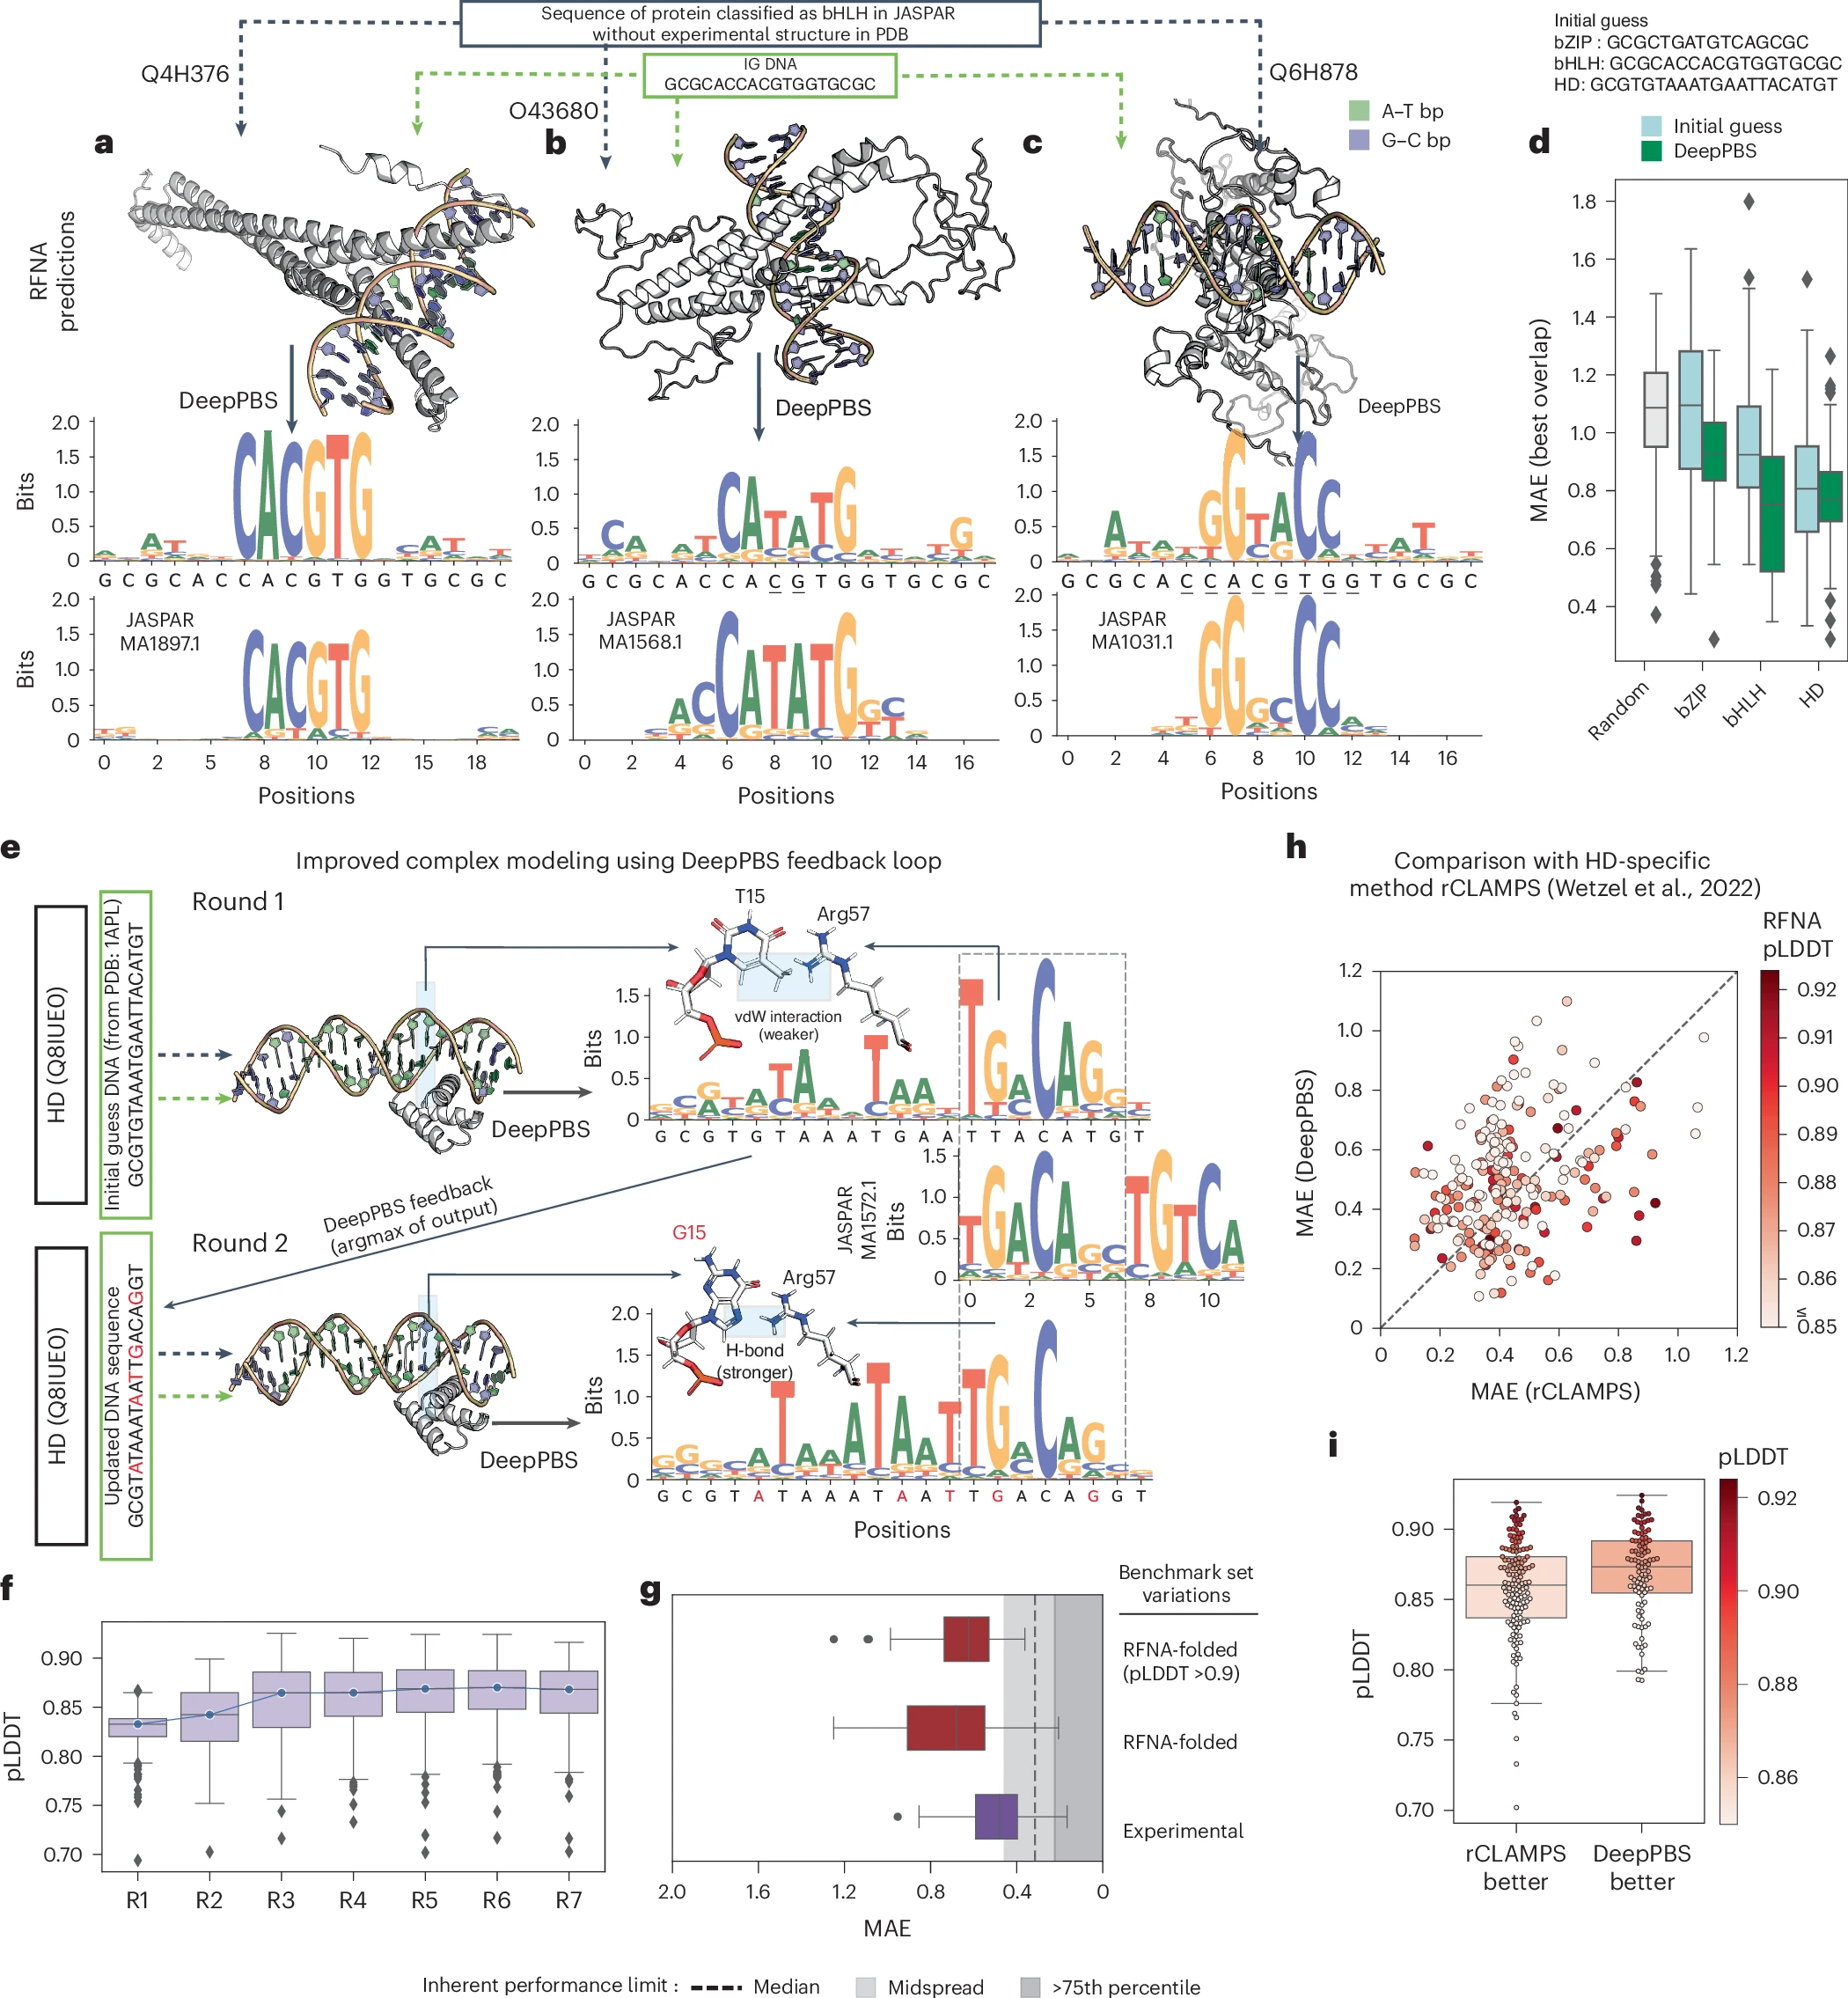
\includegraphics[width=0.8\paperwidth]{./pdnafigs/fig3.png}}
 % archetecture.png: 1149x508 px, 72dpi, 40.53x17.92 cm, bb=0 0 1149 508
        \caption[Computational cost of training RVAgene]{\textbf{Training RVAgene is reasonably scalable on CPU and even more so using hardware acceleration through GPU.} ({\bf A}) Time cost of training RVAgene for 100 epochs for datasets with varying number of genes and time points on CPU and GPU. ({\bf B}) Maximum memory utilized during training of the model on CPU an GPU for the cases in (A), inset plot: comparison of max memory used compared to DPGP for varying number of genes.}
  \label{fig:pdna3}
\end{figure}
\end{center}

\subsection{Assessing protein residue importance at p53-DNA interface}
The DeepPBS architecture permits intentional activation or deactivation of specific edges in the bipartite geometric convolution stage (Fig. 1d and Supplementary Fig. 4). Perturbing a set of edges in this manner will alter the network-predicted result. The mean absolute difference between the original and altered prediction can be used (with proper normalization) as a quantification of the impact of the perturbed set of edges in determining binding specificity (Fig. 1g, Supplementary Fig. 4 and Methods).
\par
We present results for perturbing edge sets for individual protein heavy atoms, which can also be aggregated to compute residue-level importance. As an example, we examined the protein-DNA interface of p53 (PDB ID: 3Q05), a protein crucial for regulating cancer development and cell apoptosis \citep{Joerger2008}. The tumor suppressor p53 binds to DNA as a tetramer with two symmetric protein-DNA interfaces \citep{Kitayner2010, Petty2011}. We show the RI scores (with min-max normalization applied) calculated for heavy atoms within $5\AA$ of the sym-helix (Fig. 4a). Sphere sizes in Fig. 4a denote computed RI scores, with the largest being 1 and smallest 0. Lys120 \citep{Kitayner2006} is involved in both groove readout (H-bond with G) and shape readout-based binding specificity (H-bond with backbone phosphate) (Fig. 4b). The network deems G-Arg280 \citep{Kitayner2006} bidentate H-bonds as another strong driver of binding specificity5 (Fig. 4c). Cys277 confers specificity through its thiol sulfur, accepting an H-bond in the major groove \citep{Kitayner2006} (Fig. 4d). Another important residue according to DeepPBS, Arg248 \citep{Barakat2011}, is present at the minor groove (Fig. 4e). This decision by the model is primarily based on the orientation of arginine relative to the sym-helix, which is devoid of DNA sequence information. Arg248 is attracted through enhanced negative electrostatic potential due to a narrowing of the minor groove where it binds \citep{Kitayner2010}. Among other residues in Fig. 4f, Ser241 is known \citep{Barakat2011} to be important for stabilizing Arg248. Ala276 (known for causing apoptosis upon mutation \citep{Reaz2013}) appears as another driver of specificity. This residue has been shown to be a driver of specificity via van der Waals contacts with the methyl group of T in the major groove\citep{Kitayner2006}. The binding specificity prediction of DeepPBS (Fig. 4g) aligns well with known binding patterns of p53, which follows the form RRRC(A/T)(A/T)GYYY (R denotes purine, and Y denotes pyrimidine). The interactions shown here are deemed \citep{Joerger2008, Vousden2009} as significant drivers of p53 binding.

\subsection{Comparison of residue-level importance with mutagenesis data}
We next asked whether DeepPBS-derived importance scores, which reflect the degree to which an interaction determines output binding specificity, can be considered as reliable and potentially physically significant. Although high-affinity interactions can be nonspecific \citep{Agback1998, Peterson2007}, interactions that contribute to high specificity would be expected to maximize binding affinity across different base pair possibilities. Therefore, the DeepPBS importance scores associated with these interactions should display some correlation with the corresponding binding affinities. We can test this hypothesis experimentally by using alanine scanning mutagenesis data (Supplementary Section 1). Sets of such experimental data have been made available through recent contributions\citep{Ovek2022} in the field. Utilizing these data \citep{Peng2018}, we applied suitable filtering for our context and calculated the log sum aggregated residue level importance scores using DeepPBS (Methods).
\par
A regression plot and Pearson’s correlation coefficient (PCC), as shown in Fig. 4h, illustrate the correspondence between computed values and experimental $\Delta\Delta G$ values for a diverse array of proteins and residues within the protein-DNA interface (Supplementary Table 1). The obtained PCC of 0.60 corroborates our hypothesis. It is noteworthy that the model was not trained to predict these values. These values were only obtained through perturbing the wild-type (WT) structures as input (Supplementary Fig. 4 and Supplementary Table 1). These results highlight the potential of DeepPBS as an economical guide for experimentalists who are selecting alanine scanning mutagenesis experiments to conduct at the protein-DNA interface.

\begin{center}
    \begin{figure}
    \makebox[\textwidth]{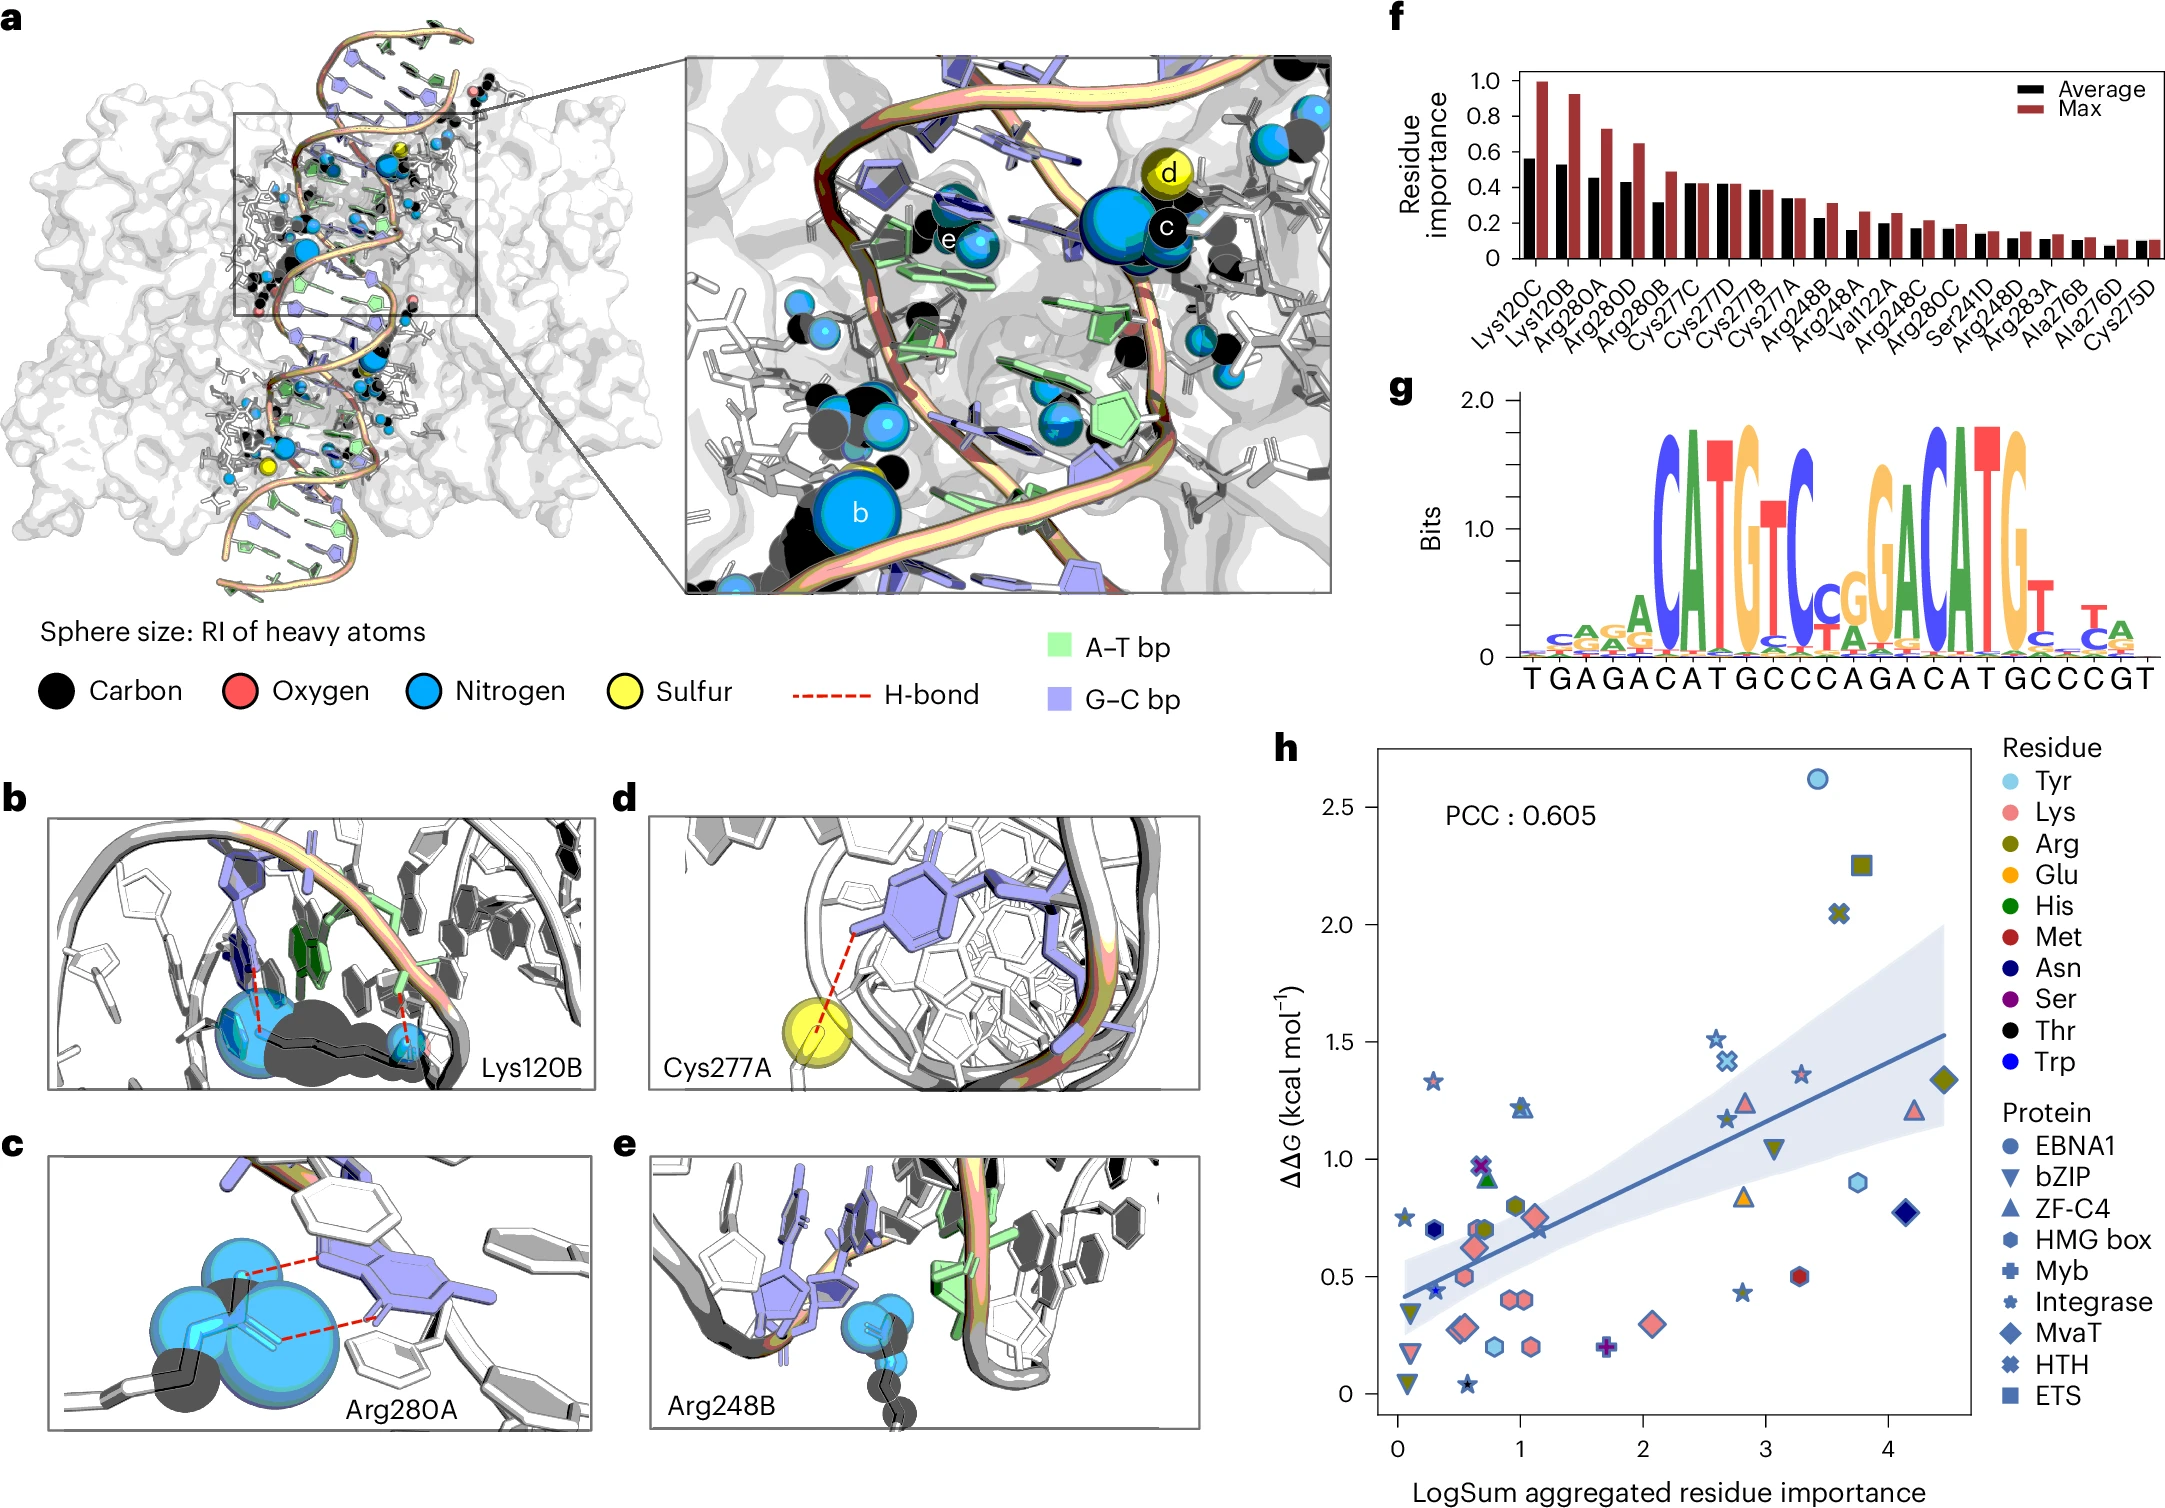
\includegraphics[width=0.8\paperwidth]{./pdnafigs/fig4.png}}
 % archetecture.png: 1149x508 px, 72dpi, 40.53x17.92 cm, bb=0 0 1149 508
        \caption[Computational cost of training RVAgene]{\textbf{Training RVAgene is reasonably scalable on CPU and even more so using hardware acceleration through GPU.} ({\bf A}) Time cost of training RVAgene for 100 epochs for datasets with varying number of genes and time points on CPU and GPU. ({\bf B}) Maximum memory utilized during training of the model on CPU an GPU for the cases in (A), inset plot: comparison of max memory used compared to DPGP for varying number of genes.}
  \label{fig:pdna4}
\end{figure}
\end{center}
\subsection{Application to designed scaffolds targeting specific DNA}
Recent work \citep{Glasscock2023} made significant progress in designing structural models of fully synthetic helix-turn-helix (HTH) protein scaffolds targeting specific DNA sequences. We applied DeepPBS to synthetically designed proteins targeting a specific DNA sequence (GCAGATCTGCACATC), named DBP5/6/9/35, respectively (Fig. 5a,e,i,m). The predicted PWMs are shown (Fig. 5b,f,j,n) and the heavy atom level RI scores are visualized for the interfaces (Fig. 5c,g,k,o). We explored qualitative agreement of these predictions with experimental results obtained from the study (Fig. 5d,h,l,p, relative binding signal of all possible single base-pair mutations obtained via flow cytometry analysis \citep{Glasscock2023} in yeast display competition assays). DeepPBS mostly correctly predicted the columns of high specificity (where the mutants show less binding that is darker red) except for a couple of cases. Some of the alternate base preference predictions by DeepPBS appear to agree with the experimental data. For example, for DBP35-position 11, DeepPBS predicts an alternate specific binding possibility to C along with the WT base A, and similarly for DBP35-position 9 and DBP5-position 7. Also, it is important to look at the flanking predictions for DeepPBS’ ability to produce sensible predictions for unbound DNA regions. For DBP9 and DBP6, the flanking predictions look remarkably uniform, which is consistent with the designed structure having mostly unbound canonical B-DNA structure. This baseline behavior is intuitive and nontrivial in this problem setting (given that there is a DNA sequence present in the design and the model has to circumvent overfitting of it). On the other hand, for DBP5 and DBP35, the flanks have a non-canonical shape with a narrow minor groove interaction with a loop region of the protein (obtained from PDB ID 1L3L). The DeepPBS prediction of a mostly A-tract preference (positions 3-8) is consistent with narrow minor groove preferred by such sequences \citep{Stefl2004}. DNA shape prediction \citep{Li2023} for the top base prediction of these columns (AAATTT) is consistent with the shape visualized in the design (Supplementary Fig. 12), showing a significant dip in minor groove width. These examples illustrate the potential for DeepPBS as a computational guide to performing expensive and laborious wet lab experiments.

\subsection{Application of DeepPBS to MD simulation of Exd-Scr–DNA system}

Owing to a fast inference time, DeepPBS can be used to analyze molecular simulation trajectories. We demonstrated how the protein heavy atom-level interpretability allows automatic detection of conformational changes in the protein-DNA interface. We applied DeepPBS to an MD simulation of the well-studied Exd-Scr-DNA system (Fig. S7a) (PDB ID: 2R5Z)\citep{Abe2015, Chiu2022, Ghoshdastidar2022, Slattery2011}. Details of the simulation method are provided in Supplementary Section 9. By computing the DeepPBS prediction over the trajectory, (Supplementary Video S1) consistent with the known binding specificity29 of the system. The
simulation trajectory was divided into 3,000 snapshots (0.1 ns apart), and the DeepPBS ensemble was applied to predict binding specificity for each snapshot. Relative importance (RI) scores were calculated for each heavy atom within 5 Å of DNA, followed by computation of max-aggregated residue RI scores. Fig. S6a shows the initial structure of the simulation, with the locations of some residues of interest marked. Residues Arg5 and His-12 of the Scr protein contribute to minor groove narrowing through electrostatic interactions, which play a crucial role in determining binding specificity \citep{Joshi2007}. 
Residues Arg58, Ile57, and Lys61 on the Exd protein interact with the major groove, driving specificity through hydrogen bonding and van der Waals interactions. In the simulation, residues Arg2, Arg3, and Arg5 on Exd contact with the flanking sequences. 

Variation of RI of the residues discussed earlier are shown in Fig. S6b,d,f. Supplementary Video 1 shows a concurrent view of changes in the network prediction as the simulation progressed, along with corresponding changes in the heavy atom RI score. Throughout the trajectory, Arg5 and His-12 on Scr consistently interact in the minor groove to drive protein-DNA binding specificity (Fig. S6e). Our model assigns stable RI scores to these residues (Fig. S6d). Arg58 strongly drives specificity by contacting G in the major groove, forming a bidentate hydrogen bond. However, after ~100 ns of simulation, the Exd recognition helix moves closer to the DNA major groove, leading to rotation of Arg58 (Fig. S6f, g) and causing a loss of strong specificity for G. Lys61 intermittently contacts the DNA through strong electrostatic interactions, leading to a gain in RI (Fig. S6f, g). 

RI scores assigned by our end-to-end deep-learning model offer an efficient alternative to traditional energy calculations, which require meticulous force-field design and energy computations. In the case of residues Arg2, Arg5, and Arg3 at the terminal loop region of the Exd protein, temporal changes in RI scores (Fig. S6b) strongly correspond to conformational changes of these residues over the simulation trajectory, as highlighted in Fig. S6c. Arg2 forms a bidentate hydrogen bond with G (~40 ns to 100 ns), which appears in DeepPBS predictions as highly specific for C (Fig. S6b). Arg5 interacts with an adjacent minor groove for most of the trajectory; however, it deviates away from the minor groove after ~210 ns, and a corresponding reduction in RI is observed. This demonstrates the ability of our deep-learning model to capture the dynamic behavior of residues and their interactions with the DNA.

DeepPBS has demonstrated its robustness and adaptability in response to both small dynamical fluctuations and conformational changes. Although the model was trained on snapshot structures and experimental PWMs, its predictions and RI scores are well-regularized and versatile, making it suitable for automated analysis of MD trajectories and designed protein-DNA complexes. These factors make DeepPBS a valuable tool for researchers working in the field of protein-DNA interactions, enabling deeper understanding and insights into the behavior of these complex molecular systems.

\subsection{Details on outliers seen on the benchmark set performance}

The outlier for the DeepPBS (Groove Readout) model is a TATA-box binding protein (TBP) bound to nucleosome bound-DNA (PDB ID: 7OH9). It is understandable that the ‘groove readout’ model will fail for this structure simply because TBP-DNA binding is known to be a primarily ‘shape readout’ driven process depending on the strong bendability and high conformational flexibility of the TATA motif \citep{simon2006}. Other than data quality limitations, another form of data limitation can be representation. For example, carboxylic acid side chains (glutamic and aspartic acids) are generally rare in biological DNA binding domains and hence in DeepPBS training data. A synthetic protein chemist should be weary of this fact, while designing domains with these residues. 

\begin{center}
    \begin{figure}
    \makebox[\textwidth]{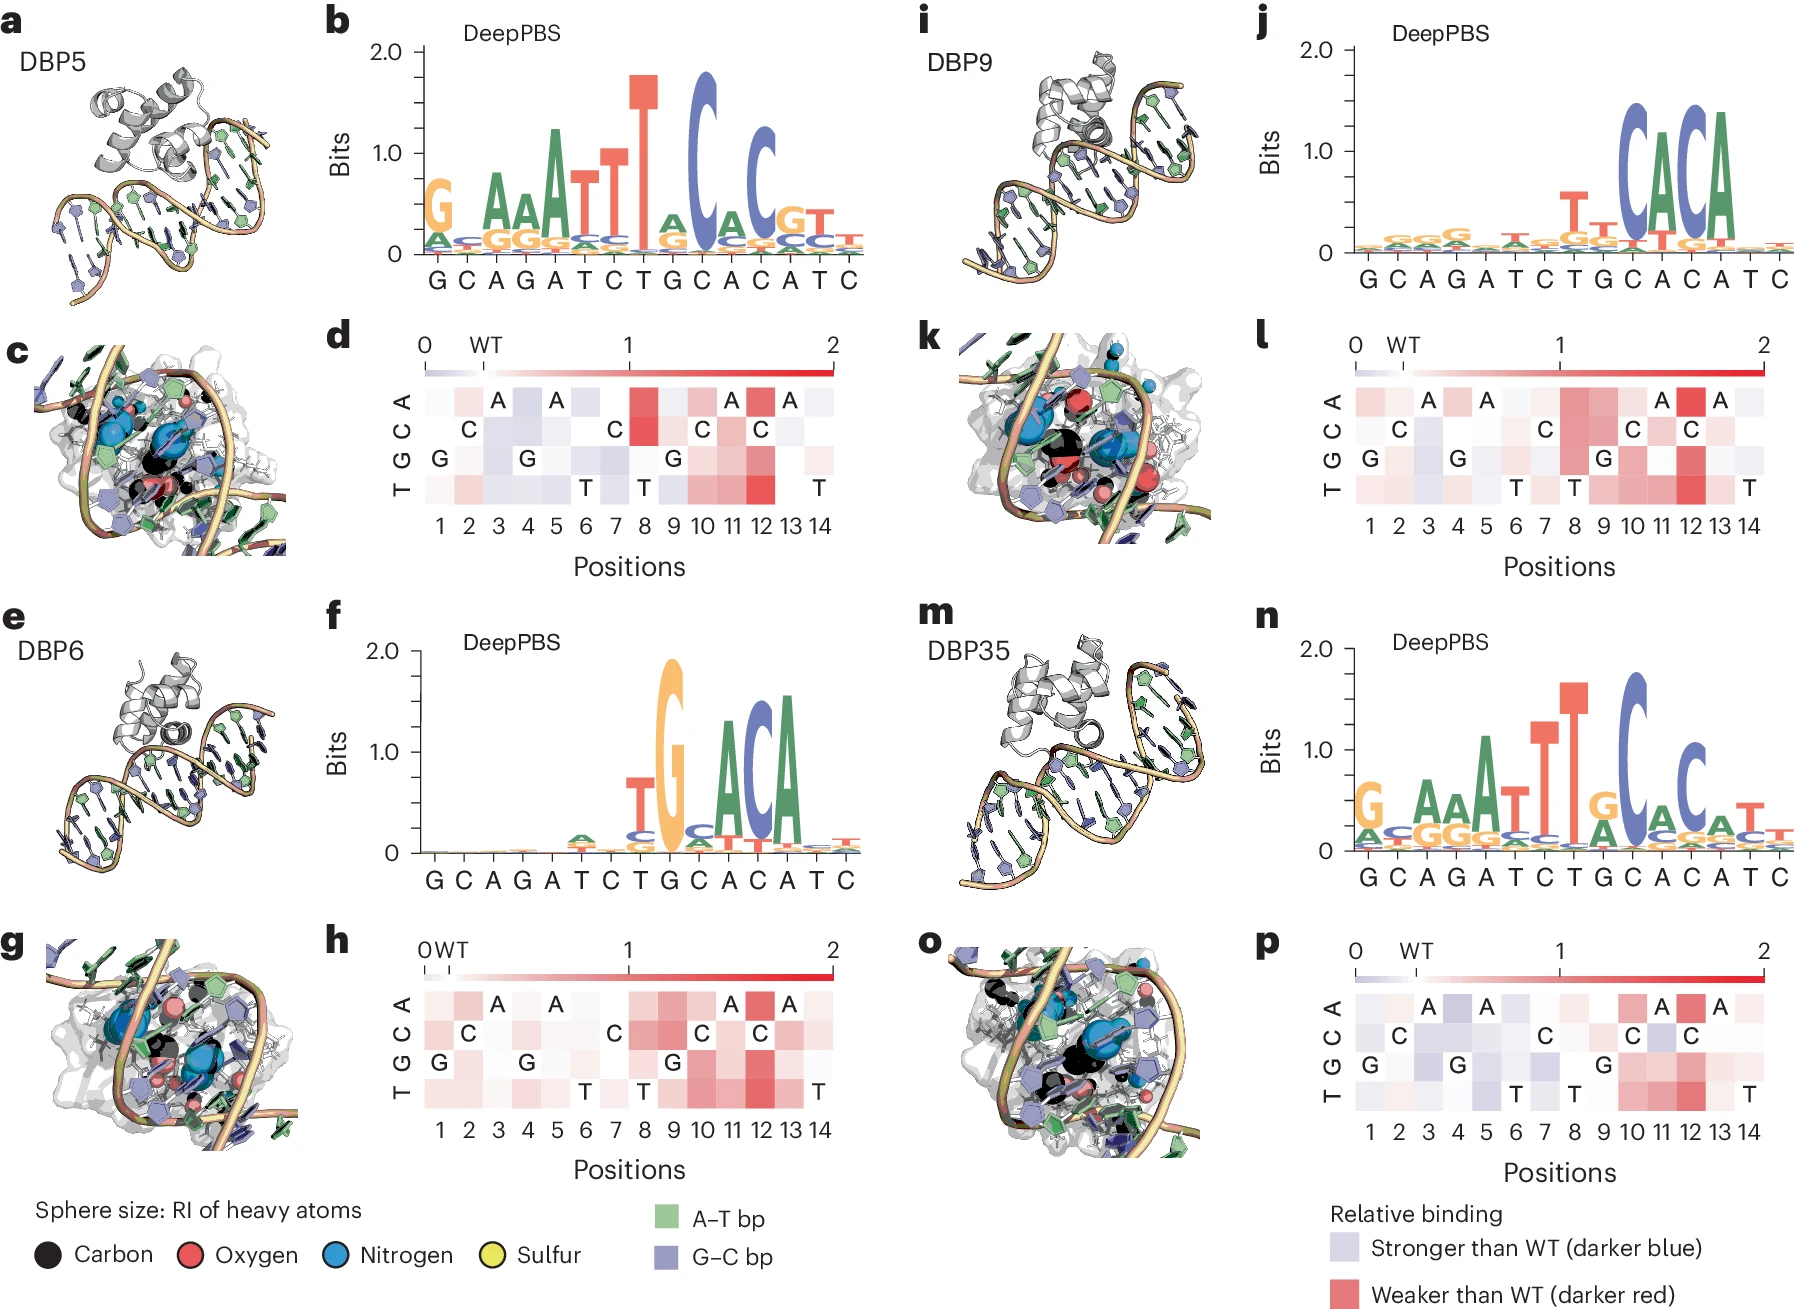
\includegraphics[width=0.8\paperwidth]{./pdnafigs/fig5.png}}
 % archetecture.png: 1149x508 px, 72dpi, 40.53x17.92 cm, bb=0 0 1149 508
        \caption[Computational cost of training RVAgene]{\textbf{Training RVAgene is reasonably scalable on CPU and even more so using hardware acceleration through GPU.} ({\bf A}) Time cost of training RVAgene for 100 epochs for datasets with varying number of genes and time points on CPU and GPU. ({\bf B}) Maximum memory utilized during training of the model on CPU an GPU for the cases in (A), inset plot: comparison of max memory used compared to DPGP for varying number of genes.}
  \label{fig:pdna5}
\end{figure}
\end{center}

%\section{Datasets}
We collected structural data from the Protein Data Bank (PDB) \citep{Berman2000} and binding specificity data from JASPAR (version 2022) \citep{Jaime2022}  and HOCOMOCO (v11 core collection) \citep{kulakovskiy2018hocomoco}. JASPAR catalogues a comprehensive set of experimental binding specificity data for proteins from different species obtained through various types of experimental platforms. HOCOMOCO consists of mainly chromatin immunoprecipitation followed by sequencing (ChIP-seq) \citep{Park2009} data for human and mouse proteins.
\par
Next, we searched for protein-DNA co-crystal structures available in the PDB (Dec 2022) for each position weight matrix (PWM) available to us using corresponding UniProt IDs. We employed DSSR \citep{lu2015dssr} to check for and annotate the existence of one contiguous double helical region in these structures. In our application, we focused on double-stranded DNA only and discarded structures that did not conform to this requirement. Base modifications were replaced by their parent base identity. A total of 1,155 PDB chain IDs were filtered into the dataset. For each structure (biological assembly containing a chain of interest) in the dataset, a corresponding PWM was paired with it. If a PWM existed in both JASPAR2022 and HOCOMOCOv11, one was randomly chosen. PWMs were trimmed to remove uninformative terminal regions with a 0.5 information content (IC) threshold. For each structure, we aligned the corresponding PWM to the DNA helix using an ungapped local alignment (Supplementary Section 2), annotating the region on the DNA helix where predictions should be made and the loss computed during training. For source code and further details of data cleaning and pre-processing, see the Data/Code Availability section.
\par
We clustered the protein chains using CD-HITv4.8.1 \citep{fu2012cd} with a 40\% sequence similarity threshold for clustering, resulting in 189 clusters. This step ensures that our dataset does not overrepresent any particular protein sequence. Next, we sampled up to five members from each cluster, prioritizing biological assemblies where the chain of interest has more contacts with the DNA region where the PWM was aligned into a fold. Full list of these memberships is available in Extended Data. We set the cutoff for alignment length to be at least five base pairs. We split this set of structures into five folds to create a cross-validation set. A schematic representation of this process is shown in Fig. S1a. Experimental and species diversity of the gathered cross-validation dataset are shown in Fig. S1b.
\par
Structures that were not included in the cross-validation dataset were resampled, selecting up to five per cluster following the same criterion. This resulted in 130 datapoints, which we used as a benchmark set. Predictions on this set were only calculated once, after finalizing all models. The family distribution of this set (Fig. 2c) differs from that of the cross-validation set (Fig. S5b).
\par
The PWM of the same protein differed slightly between JASPAR and HOCOMOCO (example shown in Fig. S1c for human estrogen receptor). This observation indicates that there is an inherent limit on what can be possibly learned, signifying noise in collected knowledge. To quantify the performance limit on the dataset based on this phenomenon, we computed the distribution of performance metrics across all unique PWMs appearing in both databases (111 cases). 
\par
Alanine scanning mutagenesis involves measuring changes in binding free energy () when performing the same binding experiment for a given protein, with a specific residue mutated to alanine. We used an already gathered dataset \citep{Peng2018} of alanine scanning mutagenesis experiments for protein-DNA structures. We filtered the dataset to make it suitable for our context. Specifically, we removed cases involving single-stranded DNA. Mutations to alanine residues with  values within 0–3 kcal/mol were retained. We removed cases in which no heavy atom of the mutated residue was within 5 Å of DNA, because our model only assigns importance scores within this range. The final dataset is summarized in Table S1.

%\section{Methods}
% \begin{center}
%     \begin{figure}
%     \makebox[\textwidth]{\includegraphics[width=0.8\paperwidth]{./pdna\_figs/fig1.png}}
%  % archetecture.png: 1149x508 px, 72dpi, 40.53x17.92 cm, bb=0 0 1149 508
%         \caption[Computational cost of training RVAgene]{\textbf{Training RVAgene is reasonably scalable on CPU and even more so using hardware acceleration through GPU.} ({\bf A}) Time cost of training RVAgene for 100 epochs for datasets with varying number of genes and time points on CPU and GPU. ({\bf B}) Maximum memory utilized during training of the model on CPU an GPU for the cases in (A), inset plot: comparison of max memory used compared to DPGP for varying number of genes.}
%   \label{fig:pdna1}
% \end{figure}
% \end{center}
\subsection{Position Weight Matrix (PWM)}
For the purposes of this study, a PWM is defined as an $N$ × 4 matrix,
where $N$ represents the length of the DNA of interest, and the four
positions correspond to the four DNA bases: adenine (A), cytosine (C),
guanine (G) and thymine (T). Each column in the PWM represents the
probabilities of the four bases occurring at that particular position.
\begin{align*}
Col_{PWM} &= [P_A, P_C, P_G, P_T]\\
P_A + P_C &+ P_G + P_T = 1
\end{align*}
\subsection{Ungapped Local Alignment}
Alignment of experimental PWMs to the corresponding co-crystal structure derived DNA is an important step for correctly annotating experimental protein-DNA structural data for model training and evaluation. This alignment needs to be ungapped and should prioritize alignment of higher IC columns from the PWM. Hence, we used an IC-weighted Pearson correlation coefficient (PCC) scoring scheme for the alignment, given by:

%%EQUATION
\begin{align}
ICWeightedPCC(Col_{PWM},Col_{DNA}) = PearsonR(Col_{PWM},Col_{DNA})\times \frac{IC(Col_{PWM})}{2}
\end{align}
where $PearsonR$ refers to a standard PCC, and $IC$ refers to the information content calculated for a probability simplex with a uniform background, in this context:
\begin{align}
IC([P_A,P_C,P_G,P_T]) = \sum\limits_{i\in[A,C,G,T]} \frac{log(P_i)}{log(0.25)}
\end{align}
%%EQUATION

%%ADD COMMENTS

\begin{pmialgorithm}[0.9\textwidth]{h!}{Ungapped Local Alignment}\vskip-2ex
        \label{algo:UngappedAlign}
        \begin{algorithmic}[1]
                \REQUIRE  $seq, pwm$ \COMMENT{Length X 4 arrays}
                \STATE  $max\_score \leftarrow -9999$
                \STATE  $opt\_i \leftarrow 0$
                \STATE  $opt\_j \leftarrow 0$
                \STATE  $opt\_k \leftarrow 0$
                \STATE  $l \leftarrow length(seq)$
                \STATE  $s \leftarrow length(pwm)$
                
                \FOR[]{$i=0,1,2,...,s-1$}
                \FOR[]{$k=0,1,2,...,s-i$}
                \FOR[]{$j=0,1,2,...,l-k$}
                \STATE  $score \leftarrow 0$
                
                \FOR[]{$col=0,1,2,...,k-1$}
                \STATE $col\_score \leftarrow ICWeightedPCC(pwm[i:i+k,:][col,:],$ \\$seq[j:j+k,:][col,:])$
                \STATE $score \leftarrow score + col\_score$
                \ENDFOR

                \IF[]{$score > max\_score$}
                \STATE $max\_score \leftarrow score + col\_score$
                \STATE $opt\_i \leftarrow i$
                \STATE $opt\_j \leftarrow j$
                \STATE $opt\_k \leftarrow k$
                \ENDIF
                
                \ENDFOR
                \ENDFOR
                \ENDFOR
                \RETURN $opt\_i, opt\_j, opt\_k, max\_score$
        \end{algorithmic}
\end{pmialgorithm}



\subsection{Representing DNA}
Our framework must consider several important factors for representing DNA. First, our model observes the structure of DNA in the input, but will predict a one-dimensional (1D) representation (a PWM). Thus, from an engineering perspective, it is beneficial to have the same number of features per base pair. Second, the input co-crystal structure derived DNA has a sequence; depending on the use case, we may or may not want our model to observe this sequence. Moreover, because experimental structural data are sparse, the co-crystal derived sequence has a strong potential for overfitting if observed by the model in the input. Therefore, in general, we want to symmetrize each base pair such that all sequence information is lost, but the global shape of the double helix is preserved. 

With these points in mind, we developed a coarse-grain symmetrized representation of DNA, where each base pair is represented by 11 points: two points for the phosphate moiety on each strand, two points for the sugar moiety, four points for the major groove, and three points for the minor groove. Major and minor groove points are placed symmetrically in the base-pair plane, so that they do not possess any particular base identity but roughly correspond to the major and minor groove chemical positions known \citep{Chiu2023} to be used for base readout. The phosphate moiety is represented by the coordinate of the phosphorus atom. The sugar moiety is represented by the average coordinate of all sugar heavy atoms. The three minor groove points divide the line segment connecting the two C1' atoms into four equal segments. The base-pair plane is determined by the triangle connecting the two C1' atoms and point O (average of atoms N1 and N9). Next, we move perpendicular (to the minor groove line segment) in this plane from either C1' for 3.75 \AA\  and expand the line segment by another 1.54 \AA\  in either direction. The line segment is divided into five equal segments to determine positions of the four major groove points. Additionally, the central two major groove points are shifted by an additional 1 \AA\ . This geometric construction is based solely on domain knowledge; no learning is employed to estimate any parameter. \hyperref[fig:pdnaS2]{Fig. S2a} shows a schematic representation of this process for an A-T base-pair. The only base atoms used for this process are N1 and N9, making it agnostic of base identity. 

\hyperref[fig:pdnaS2]{Fig. S2b} shows an example transformation of a DNA structure to a symmetrized helix (sym-helix) using the described process. \hyperref[fig:pdnaS2]{Fig. S2c} shows one C-G base pair overlayed with sym-helix points computed for the corresponding base pair. As a result, the DNA structure is represented as $G^d = (V^d, X^d, N^d)$ .  $V^d$ represents coordinates of the sym-helix points, and $X^d$ represents point-level DNA features, which reflect a one-hot encoded annotation of the 11 positions in the symmetrized base-pair representation. If desired, we can reintroduce the DNA sequence (`DeepPBS with DNASeqInfo' model) by including base-pair-specific chemical group features for each point to $X^d$, as \citep{Chiu2023}. For each point , we also define an interaction vector $N^d_v$. These vectors act as reference directions in the base-pair frame. They are used to compute relative orientation-based features coupled with vectors $N^p$ on the protein graph (refer to Section 4). For the phosphate point, this vector is the average direction of the two double-bonded oxygens; for the sugar point, this vector is the direction of the C4'-C5' bond. For the seven major and minor groove points, these directions are determined by connecting each point to the centroid of the heptagon formed by these points. \hyperref[fig:pdnaS2]{Fig. S2e} shows the arrangement of these vectors on a sym-helix. These directions do not encode any base-specific information and only serve to inform the relative orientation of a sym-helix point in the context of binding. In addition, we include 14 DNA shape features \citep{Lavery2009, Lu2008, lavery1989defining} denoted as $X^s$, which are base-pair level features (\hyperref[fig:pdnaS2]{Fig. S2d}). These features are: buckle, shear, stretch, stagger, propeller twist, opening, shift, slide, rise, tilt, roll, helix-twist, major groove width, and minor groove width. 3DNAv2.3 \citep{Lu2008} and Curves5.3 \citep{Lavery2009, lavery1989defining} were used to calculate these values. Mean-padding was used to offset inter-base-pair features (shift, slide, rise, tilt, roll, helix-twist).

\subsection{Representing protein}

In our framework protein is viewed as a spatial graph $G^p = (V^p, X^p, E^p, N^p)$  where the
coordinates of the heavy atoms constitute the vertices $V^p$. For each vertex $v \in V^p$  we define
a set of features $X^p\_v$ which include one hot encoded atom type, solvent accessible surface area
of the atom, charge, radius, circular variance (7.5 $\AA$) and Atchley factors \citep{Atchley2005}. The edges $E^p$ of the protein
graph  are determined by the covalent bonds i.e. if  vertices $u$ and $v$ have
a covalent bond between them then $(u,v) \in E^p$. The edges are unordered. Lastly to encode
directionality of protein side chains we encode a unit vector $N^p\_v$ for each vertex $v$ computed by
averaging the directions of convalent bonds associated with each heavy atom. 

\subsection{DeepPBS architecture}
The architecture of DeepPBS is modular. First, the \textbf{ProteinEncoder} module applies spatial graph convolutions on the protein graph to aggregate neighborhood environment information for each protein heavy atom. Initially, a fully connected embedding layer is applied to $X_v^p \forall v \in G^p$, which expands the dimensionality of $X_v^p$ to 10 dimensions. Four layers of crystal graph convolutions (CGConv)\citep{Xie2018} are applied. The first two layers use only covalent bond edges, and the next two layers use distance-based edges with a 4\AA\  radius. The mathematical description of the message-passing scheme for CGConv is as follows:   
%%EQUATION
\begin{align}
X_v^p \leftarrow X_v^p + \big{(}\frac{1}{|\cN(v)|}\big{)}\sum\limits_{u\in\cN(v)}
\sigma(z_{uv}W_f + b_f)\odot g(z_{uv}W_s + b_s)
\end{align}
 
where $\cN(v)$ denotes the neighbors of $v \in V^p$ , and $z_{uv} = [X^p_v,X^p_u,e_{uv}]$ denotes the concatenation of target node features, source/neighboring node features, and edge features (here, the distance between u and v). In addition,  $\sigma$ denotes the sigmoid function, and $g$ denotes the softplus function. A Rectified Linear Unit (ReLU) \citep{Agarap2018} activation function is applied after each round of graph convolutions. This marks the end of the ProteinEncoder module.

The sym-helix point features $X_v^d$ are embedded into a 10-dimensional (10D) space using fully connected neural network layers and are used in the next module, the \textbf{Bipartite Geometric Network (BiNet)}. In this module, aggregated information on $G^p$ are pulled onto the sym-helix by performing geometry-aware bipartite convolutions. We use a modified version of point pair feature convolutions (PPFConv) \citep{Deng2018}, which we call a bipartite ResidualPPFConv. The message-passing update scheme associated with it is as follows: 
%%EQUATION
\begin{align}
X_v^d \leftarrow X_v^d + \gamma_\theta\bigg{(}\sum\limits_{u\in\cN(v),u\in V^p}h_\theta \big{(}
        x_u^p, ||d_{uv}||, \angle(N_v^d, d_{uv}), \angle(N_u^p,d_{uv}), \angle(N_v^d, N^p_u)
\big{)}
\bigg{)}
\end{align}

where $d_{uv}$ denotes the line segments connecting a sym-helix point $v$ and a protein heavy atom point $u$. $h_\theta$ is a transformation parametrized by fully connected neural networks. We set $\gamma_\theta$ to be the identity transformation. Four separate ResidualPPFConvs are applied for the major groove, minor groove, phosphate, and sugar points, respectively (from neighbors within 5 \AA), followed by ReLU activation. At this stage, we have aggregated all local chemical and geometric interaction contexts onto the sym-helix.

The final module is the \textbf{CNN-Predictor} module. We flatten the helix into a 1D base pair-level representation and apply a Multi Layered Perceptron (MLP) to reduce the dimensionality for each base-pair to 32. We concatenate precomputed helix shape features to aggregated base pair-level features. This step allows the network to make connections/correlate patterns between the aggregated information from BiNet and the global shape of the helix. We apply two rounds of 1D convolutions of filter size 3 with a stride of 1. We also apply relevant padding and set output feature size of 8, followed by ReLU activation, making the effective field of view five base-pairs. Next, we apply an MLP for each base-pair to generate logits for predicted base probabilities $([L_A,L_C,L_G,L_T])$ for corresponding base-pairs. We apply a SoftMax \citep{Bridle1990} activation to generate the output DNA base probabilities $([P_A,P_C,P_G,P_T])$. A global temperature parameter ($T_{glob}$) is learned for SoftMax through the training process. \hyperref[fig:pdnaS3]{Fig. S3} schematically describes the DeepPBS architecture.
\begin{align}
P_i = \frac{\frac{L_i}{e^{T_{glob}}}}{\sum\limits_{j\in[A,C,G,T]}\frac{L_j}{e^{T_{glob}}}} \forall i \in \{A,C,G,T\}
\end{align}
%%EQUATION
% 
% \begin{center}
%     \begin{figure}
%     \makebox[\textwidth]{\includegraphics[width=0.8\paperwidth]{./pdna\_figs/fig2.png}}
%  % archetecture.png: 1149x508 px, 72dpi, 40.53x17.92 cm, bb=0 0 1149 508
%         \caption[Computational cost of training RVAgene]{\textbf{Training RVAgene is reasonably scalable on CPU and even more so using hardware acceleration through GPU.} ({\bf A}) Time cost of training RVAgene for 100 epochs for datasets with varying number of genes and time points on CPU and GPU. ({\bf B}) Maximum memory utilized during training of the model on CPU an GPU for the cases in (A), inset plot: comparison of max memory used compared to DPGP for varying number of genes.}
%   \label{fig:pdna2}
% \end{figure}
% \end{center}
\subsection{Training, cross-validation, and benchmarking}

Five models were trained for each of the four types: DeepPBS, DeepPBS GrooveReadout, DeepPBS ShapeReadout, and DeepPBS with DNA SeqInfo. Each model was trained on four folds of the constructed cross-validation set. Training was conducted for 50 epochs with early stopping on an NVIDIA RTX A4000 using an Adam \citep{Kingma2017} optimizer, with a learning rate of 0.001 and weight decay of 0.0001. Hyperparameters were selected based on domain knowledge and training curves. For every datapoint, two forward passes were made to account for reverse complement predictions for both strand directions (with relevant index transformations for input; refer to Data/Code Availability). Outputs were concatenated, and MAE loss was calculated with ground truth (corresponding PWM and its reverse complement concatenated). Predictions were made on the corresponding fifth/validation fold with each model to gather predictions for all datapoints in the 5-fold dataset. These predictions were used to report metrics in \hyperref[fig:pdnaS5]{Fig. S5a-c}. 

For benchmarking purposes, ensemble averaged (of the five trained cross-validation models) predictions are used \blue{Fig. 2.3a-d}. The ensemble is also used for results presented in \blue{Fig. 2.4, 2.5, 2.6}, and \blue{Fig. S5b,d, S6, S7, S8, and S9}. All core DeepPBS code was written in python3.9+ with various pythonic dependencies (full list available at \href{https://github.com/timkartar/DeepPBS}{GitHub}). Packages used for geometric deep learning are pytorch1.12+ and torch-geometric (pyg v2.0+).

\subsection{Performance metrics}

Performance metrics used in this chapter are MAE and RMSE, defined as 
%%EQUATION
\begin{align*}
\text{MAE}(Y, Y^{pred}) &= \frac{1}{N} 
\sum\limits_{i\in\{0,..,N-1\}} \sum\limits_{b\in\{A,C,G,T\}} |Y_{ib} - Y_{ib}^{pred}|\\
\text{RMSE}(Y, Y^{pred}) &= \sqrt{\frac{1}{N} \sum\limits_{i\in\{0,..,N-1\}} \sum\limits_{b\in\{A,C,G,T\}} (Y_{ib} - Y_{ib}^{pred})^2}
\end{align*}

$N$ refers to the number of columns in the PWMs being compared. Both metrics follow ‘the lower the better’ principle. They are not independent but have different properties. 

\subsection{Additional discussion on behavior of metrics}

To get a better perspective of the behavior of MAE metric, we demonstrated of how the MAE metric behaves for various different target PWM columns and possible predictions (\hyperref[fig:pdnaS10]{Fig. S10a}). The predictions are of three forms, based on interpolated values of a variable $x\in[0,1]$. They are as follows: %%EQUATION
\begin{align}
[1-x,0,x,0], [x, \frac{1-x}{3}, \frac{1-x}{3}, \frac{1-x}{3}], [\frac{1-x}{3}, \frac{1-x}{3}, \frac{1-x}{3}, x]
\end{align}
. These demonstrations, although they do not form an exhaustive set, but gives an idea of the behavior of the MAE metric. Based on these plots and taking into account the inherent performance limit computed for this metric, we can consider values less than 0.8 to be of reasonable agreement and below 0.6 to be in good agreement. Although, we do note that these values should not be set in stone as the problem in question is a regression problem as opposed to binary classification.

Some further thoughts on this matter: In theory, the uniform prediction [0.25, 0.25, 0.25, 0.25] can be regarded as a bad prediction, because a naive model can always predict such a value. This prediction will perform well for highly non-specific binders (e.g., cases like \hyperref[fig:pdnaS8]{Fig. S8}) but will fail for highly specific binders. However, the one-hot prediction [1,0,0,0] can also be a naive (bad) prediction for this problem setting. It is the case when the sequence present in the co-crystal structure itself is the output, e.g., for the sequence ACG: [[1,0,0,0],[0,1,0,0],[0,0,1,0]]. For experimentally determined structures, this prediction will generally perform well, especially for highly specific binders, but will fail for nonspecific binders. Ultimately, we wanted to create a general model that can handle specific binders and non-specific binders. So, we need a target metric to strike a balance between both scenarios. Therefore, in our opinion, looking at the predictive performances in context of the alignment scores of the co-crystal structure derived sequence with the target PWM gives a clearer picture. This has now been added (for the benchmark set) to the manuscript as \hyperref[fig:pdnaS10]{Fig. S10b}.

We choose a continuous distance metrics like MAE over statistical measures like PCC (Pearson R) or SCC (Spearman R) because they are not very robust with only four (linearly dependent) points (well-known result in the statistics community \citep{Bonett2000, McIntyre1938}. In our observation, SCC can only take a few discrete values in this scenario and can sharply change for a very small change of values that change the rank order. The PCC metric, although it takes continuous values, is affected by similar non-intuitive situations. This is easy to demonstrate by considering the following three slightly altered predictions:
\\
PCC([0.5,0.5,0,0], \textbf{[0.25,0.25,0.25,0.25]}) = Undefined\\
PCC([0.5,0.5,0,0], \textbf{[0.23,0.24,0.26,0.27]}) = -0.9487\\
PCC([0.5,0.5,0,0], \textbf{[0.27,0.26,0.24,0.23]}) = 0.9487\\
(calculated using scipy.stats.pearsonr() function)

Intuitively, all three predictions are of similar caliber. However, the PCC metric paints a dramatically different picture. MAE on the other hand produces values of 1, 1.06 and 0.94. This is much more nuanced and intuitive. We can also easily construct other non-intuitive situations for PCC. For example, if the target is [0.1,0.2,0.3,0.4], any monotonically increasing prediction will have a high PCC value.

PCC([0.1,0.2,0.3,0.4], \textbf{[0.001,0.002,0.003,0.994]}) = 0.776

This gives the impression that this prediction is quite good, while in reality, it is almost just a one-hot prediction. MAE on the other hand produces a value of 1.187 which depicts a bad prediction.

\subsection{Additional details associated with application of DeepPBS on predicted structures}
%% CHECK LINKS

\textbf{Running rCLAMPS}: We ran the rCLAMPS model with default parameters provided by the model’s authors according to instructions provided through their GitHub.
\\
\textbf{Running RoseTTAfoldNA (RFNA)}: We ran the RFNA model with default options and model weights (version: April 13, 2023 v0.2) as provided by the authors through their GitHub.
\\
\textbf{Trimming unstructured regions from full-length homeodomain (HD) sequences}: For the analysis in \hyperref[fig:pdna3]{Fig. 2.4e-i}, full-length HD sequences were first trimmed to remove unstructured regions, while retaining the main Homeobox domain of interest (rCLAMPS also applies the same process in its pre-processing). This step was achieved by HMMERv3.4 \citep{Finn2011} using the ‘homeobox.hmm’ file provided by the rCLAMPS repository. 
\\
\textbf{MM-PBSA vacuum energy calculation}: For each PDB file, we generated a topology file and a run-parameter file using Gromacs 2020.3 to define the force fields amber14sb for protein and parmbsc1 for DNA. These files were used as input for g$\_$mmpbsa to calculate the potential energy in a vacuum. The dielectric constant of the solute was set to 8. 
\\
\textbf{Dataset}: We obtained UniProt protein sequences for three different families, bZIP (homodimers), bHLH (homodimers), and homeodomain (HD) (heterodimers excluded), for cases with a corresponding unique JASPAR entry and no experimental structure for the complex. RFNA predictions that could be successfully processed by DeepPBS pre-processing steps were fed into DeepPBS for specificity prediction (n=49 for bHLH, n=50 for bZIP, n=236 for HD family members).
\\
\textbf{Choice of initial guess (IG) DNA}: The IG DNA for the bHLH family was chosen as ‘GCGCACCACGTGGTGCGC’, which has a center E-box motif (‘CACGTG’) that is known \citep{demartin2021} to be a bHLH family target. The IG DNA for the bZIP family was chosen as ‘GCGCTGATGTCAGCGC’ (based on human CREB1 motif MA0018.4). The IG DNA for the HD family was chosen as ‘GCGTGTAAATGAATTACATGT’, based on DNA from PDB ID 1APL. 
\\
\textbf{Details on metric calculation for \hyperref[fig:pdna3]{Fig. 2.4d}}: We calculated MAE (best full overlap) for predictions in \hyperref[fig:pdna3]{Fig. 2.4d} against corresponding JASPAR annotations. As a baseline (apart from random predictions drawn from uniform), we calculated the MAE (best full overlap) for the one-hot PWM determined by the IG DNA against the corresponding JASPAR annotation. For the bHLH and HD families, the IG DNA was closer to experimental data than to random baseline (\hyperref[fig:pdna3]{Fig. 2.4d}).
\\
\textbf{pLDDT score}: (RFNA-predicted LDDT (Local Distance Difference Test) score \citep{Mariani2013}). The LDDT score measures the similarity between a predicted and reference structure. When predicting a complex structure, RFNA predicts an LDDT score (pLDDT). These pLDDT scores were shown \citep{baek2024na} to be well correlated with the true LDDT of RFNA predictions. Thus, the pLDDT can be taken as a measure of quality of a complex generated by RFNA.
\\
\textbf{Comparison of DeepPBS and rCLAMPS}: There are several qualitative advantages to the DeepPBS approach. First, rCLAMPS uses structural mapping for HD-DNA binding to predict specificity for a given HD sequence. This structural mapping leads to a specificity output of exactly six 6 base pairs (bp). DeepPBS is functionally not limited to only predicting a 6-base pair core and can predict preferences in the flanks (\hyperref[fig:pdna3]{Fig. 2.4e}). Second, rCLAMPS is restricted to predicting monomer preferences (although HD proteins can often bind as dimers; see, e.g., \hyperref[fig:pdnaS6]{Fig. S6a}). In contrast, DeepPBS is able to handle biological assemblies. Third, DeepPBS is not limited to a specific family. For quantitative comparison, we compare the aspects that are achievable by rCLAMPS, namely, 6mer specificity predictions for monomer HD proteins.
\\
\textbf{Metric computation for comparison with rCLAMPS}: We ran rCLAMPS (github commit version 32a94edb65e87c6d038823dc34c4bcf6e1071b7b) on the set of monomer HD proteins (with unavailable complex structure, i.e. not part of RFNA or DeepPBS training). We computed the MAE (best overlap) values for rCLAMPS predictions against the corresponding JASPAR entry of experimental data, and compared these values to the MAE values of the best 6-mer overlap for DeepPBS predictions. In this case, for each datapoint, one of round 4-7 prediction was chosen. This choice was based on maximizing corresponding protein-DNA contact count (5 \AA cutoff) of input RFNA predicted structure. 
\\
\textbf{Folding benchmark set datapoints with RFNA}: We refolded all the benchmark set datapoints with RFNA, for results presented in \hyperref[fig:pdna3]{Fig. 2.4g}. 108/130 RFNA predictions produced pre-processable results. Out of them a few of were not able to place the protein near the DNA helix properly. So, we filtered an atom-to-atom contact count (within 5 \AA) of greater than 500 contacts between protein and DNA to filter this set producing a set of size 98. The high confidence set among these are taken as predictions for which the RFNA pLDDT was greater that 0.9.

\subsection{Molecular Dynamics (MD) simulation of Exd-Scr–DNA system}
We conducted MD simulations on the Drosophila Extradenticle (Exd)-Sex combs reduced (Scr) system, with the dimer bound to its target DNA, using the co-crystal structure (PDB ID: 2R5Z). AlphaFold2 predictions of the proteins were aligned to the PDB structure to create an initial structure of the simulation. This process aided in filling in the missing linker residues in the biological assembly. The simulation was executed using the Gromacs \citep{Abraham2015} 2020.3 software package. Protein interactions were modeled with the amber14sb \citep{Maier2015} force field, and DNA interactions were modeled with the parmbsc1 \citep{Ivani2016} force field. The pdb2gmx program from Gromacs was used to generate topological information for the simulation. The -his flag was used to protonate both N$\delta$ and N$\epsilon$ atoms of the His-12 residue for the system with protonated His-12. All complexes were solvated using the explicit TIP3P water model. The negative net charge of the Exd-Hox-DNA complex was neutralized by adding positively charged Na+ counterions, along with negatively charged Cl- counterions, to reach a final NaCl concentration of 150 mM that approximates the physiological concentration. The GROMACS 2020.3 genion program was used to place these counterions throughout the box. 
\par
The protein-DNA complex was energy-minimized with steep descent energy minimization for 2,000 steps to relax the structure and remove any steric clashes. Next, we performed three rounds of gradual NVT (constant Number of particles, Volume, and Temperature) equilibration for 10 ps to slowly heat the prepared system to 300K and 1 round of NPT (constant Number of particles, Pressure, and Temperature) to equilibrate the pressure of the system to 1 bar for 700ps. These equilibration rounds were used to adjust the whole system to biological conditions before starting the production simulation. The production simulation for the system was run for 300 ns in the isobaric–isothermal ensemble, where the pressure was maintained at 1 bar and temperature at 300K. The integration time step of 2 fs was used for all calculations. The Verlet cutoff scheme was used for all calculations. Long-range electrostatic interactions were computed using the Particle Mesh Ewald method \citep{Darden1993} from the GROMACSv2020.3 package, with a 12\AA cutoff. Nonbonded van der Waals interactions were calculated with a 12\AA cutoff. The LINCS \citep{Hess1997} algorithm from the GRPMACSv2020.3 package, was employed to constrain all bonds.The MD simulation trajectories were generated as part of a recent study exploring effects of minor groove linker histidine protonation \citep{Jiang2023}.
\\
\subsection{Measures ensuring prevention of overfitting to protein sequences}
We took several steps to prevent the model to be overfit on protein sequences. The cross-validation fold creation script (see Code Availability) took care to keep members of the same cluster in the same fold (except a handful ($<4\%$) got split randomly to keep the fold sizes same). Full description of these splits is available (see Data Availability) and the code for this process is available (see Code Availability). In addition, no more than five samples were chosen per cluster into a fold. This ensures prevention of over representation. Furthermore, the input to DeepPBS is purely structural and physico-chemical, and does not contain the sequence representation. These structures may demonstrate different spatial conformations interacting with potentially different DNA sequence/shape and randomly picked target PWM from JASPAR or HOCOMOCO. These guardrails in architecture and all of these variations, even for similar protein sequences, makes the model less prone to overfit on protein sequences. 
\\
\subsection{Bipartite edge perturbation and protein heavy atom importance score calculation}
Supplementary \hyperref[fig:pdnaS4]{Fig. S4} schematically describes the bipartite edge perturbation process for calculating protein heavy atom (say, atom a) importance scores. Briefly, the prediction is calculated twice: once (say, $Y_a$) while considering edges corresponding to the protein heavy atoms, and again (say, $Y_{\sim a}$) while masking the same edges. This process results in differences in predictions, which can be calculated using the mean absolute difference measure. On their own, these values may not be meaningful, but they can be normalized to the 0–1 range by dividing by the maximum value within a structure. The normalized values, RI scores, signify how much the specificity prediction is influenced by interactions made by the corresponding heavy atom. Depending on the downstream use, RI scores can be aggregated at the residue level using either the average, max or sum aggregations. Mathematically,
\begin{align} 
RI_\alpha = 
\frac{\text{MAE}(Y_a,Y_{\sim a})}
{max_{\{b\in all\ atoms\}}\text{MAE}(Y_b,Y_{\sim b})}
\end{align}
\par
Computationally, this process is like measuring the effect of a deactivating mutation, which is why we hypothesized that, at a residue level, these scores could correlate with alanine scanning mutagenesis data. For comparison with alanine scanning mutagenesis experiments (\hyperref[fig:pdna4]{Fig. 2.5h}) at a residue level, the log sum aggregated importance score was calculated. For each atom a of a residue r in the protein–DNA interface, let the calculated RI be RIa. Then, this value is calculated as
\begin{center}
LogSum aggregated residue importance($r$) = $log_2(1 + \sum\limits_{a\in r}RI_\alpha)$ %%EQUATION
\end{center}
Structure visualizations presented were produced using PyMOL2.5 \citep{pymol}.

\subsection{Description of competitor assay for quantifying designed proteins’ binding specificity}

Glasscock et al. \citep{Glasscock2023} used a yeast display assay to quantify binding of their designed proteins. The proteins were expressed by integrating the corresponding synthetic oligonucleotide to a yeast surface expression vector. Yeast cells expressing designed proteins on their surface were labeled with biotinylated dsDNA targets, streptavidin–phycoerythrin and anti-c-Myc fluorescein isothiocyanate in a 96-well plate format, after which a binding signal was quantified on an Attune NxT flow cytometer. Excess addition of a competitor nonfluorescent target DNA reduces this binding signal. Thus, scanning single mutations for each position was possible through the competitor producing the data shown in \hyperref[fig:pdna5]{Fig. 2.6d,h,l,p}.
\\
\subsection{DeepPBS webserver}
DeepPBS is available as a webserver at https://deeppbs.usc.edu. The webserver provides the functionality of the DeepPBS method of predicting a PWM on the basis of the structure of a protein–DNA complex. The structure can be uploaded as a PDB or macromolecular crystallographic information file. The webserver provides a documentation for users.

%\section{Discussion}

Computationally identifying which DNA sequences, a given protein will bind to remains a challenging question. Although proteins from certain DNA-binding families, such as homeodomain \citep{Christensen2012, Dror2014, noyes2008analysis, Wetzel2022} and C2H2 zinc finger proteins \citep{Wetzel2022, Persikov2014, persikov2009predicting, meseguer2020prediction, Persikov2011, persikov2015systematic} have been studied extensively in this regard, a generalized model of binding specificity remains elusive. This complexity emanates, in part, from the pivotal role that the protein and DNA conformation or shape play in the context of binding specificity. For example, TBX5 undergoes an $\alpha$- to $3_{10}$-helix conformational change when interacting with DNA. Despite the energy penalty, this transformation, in conjunction with an appropriately matching DNA shape, instigates a strong phenylalanine-sugar ring stacking, thereby facilitating binding \citep{Stirnimann2010}. Another example is the Trp repressor protein, which exhibits an almost entirely geometry-driven binding specificity. This protein only forms direct and water-mediated H-bonds with the backbone phosphates \citep{Otwinowski1988}, and the DNA shape required for optimal binding gives rise to sequence specificity. Capturing such interactions and how they lead to binding specificity with protein information alone is complicated and cannot be understood in a sequence space alone \citep{Chiu2023, Zhou2015}. Furthermore, for many protein families, the protein monomer is insufficient \citep{Kitayner2006} for binding; a biological assembly, potentially with other interaction partners \citep{Nair2003}, is often necessary.
\par
DeepPBS achieves generality across protein families with the tradeoff of requiring a docked sym-helix, representing a significant step toward solving the larger unsolved problem. As demonstrated in this work, coupling DeepPBS with attempts to model protein–DNA complexes provides a significant step forward in predicting binding specificity across families, based solely on protein information.
\par
DeepPBS allows exploration of exciting future possibilities, including the creation of DNA-targeted protein designs that could potentially contribute to therapeutic advancements. DeepPBS could serve as a preliminary screening tool for devised candidate complexes, ensuring their specificity to the intended target DNA sequence before any costly experimental validations. Moreover, recent studies have shown that transcription factor–DNA binding can energetically favor mismatched base pairs \citep{afek2020dna}. Given the combinatorial complexity of possible hypotheses, deciding which DNA mismatch experiments to perform to discover more such instances poses a significant challenge. Although there is currently a lack of training data for base-pair mismatches, the DeepPBS architecture, in theory, could facilitate the prediction of mismatched base-pair binding specificity. This approach could assist in deciding which experiments to conduct.
\par
In summary, we have introduced a computational framework that distills the intricate structural nuances of protein$-$DNA binding and bridges this understanding with binding specificity data, effectively connecting structure-determining and specificity-determining experiments. The DeepPBS architecture allows inspection of family-specific ‘groove readout’ and ‘shape readout’ patterns and their effects on binding specificity. Although structure prediction methods like RFNA \citep{baek2024na}, MELD-DNA \citep{Esmaeeli2023} and AlphaFold3 \citep{Abramson2024} can predict a complex from given protein and DNA sequences, they cannot provide insights into binding specificity. The development of these computational methods for structure prediction expands the need of an approach like DeepPBS to derive protein–DNA binding specificity. DeepPBS operates on predicted complexes to yield the binding specificity of the system, thereby guiding the further improvement of modeling techniques for protein–DNA complexes. 
\par
DeepPBS was trained only on experimentally determined structures and binding specificity data. We have shown, it can be used to make predictions based on predicted structures. However, there is a concern of prediction error propagation, specially if this kind of prediction based on prediction is done iteratively. This arises from the simple fact that structure prediction methods (although becoming increasingly accurate) are not perfect. Similar concern also needs to be acknowledged if one is looking to train DeepPBS (or a similar model) on predicted complexes. However, there is still some advantage in doing so, specificially for the binding specificity prediction task. The advantage arises from having a lot more binding specificity data than structural data. The large surplus of experimentally determined binding specifity data can be used to inform the model. Training on predicted complexes with experimental specificity data thus could still have some advantages.

\par
DeepPBS, despite its generality, exhibits performance comparable to the recently described family-specific method rCLAMPS \citep{Wetzel2022}. In addition to modeled complexes for biologically existing systems, DeepPBS is also applicable to in silico synthetically designed proteins that target specific DNA sequences.
\par
DeepPBS-derived RI scores are biologically relevant. They can be aggregated at a protein residue level, aligning with alanine scanning mutagenesis experimental data. Another advantage of DeepPBS is its speed in predicting binding specificity. Specifically, DeepPBS only requires a single forward call through the model (no required database search or multiple sequence alignment computation), making it suitable for high-throughput applications such as analyzing MD simulation trajectories (Supplementary \hyperref[fig:pdnaS6]{Fig. S6}). In this context, DeepPBS is robust to small dynamical fluctuations and can respond to conformational changes.
\par
The current version of DeepPBS has inherent limitations. It is tailored for double-stranded DNA and is not yet applicable to single-stranded DNA, RNA or chemically modified bases. However, there is potential for extending the model to accommodate these different scenarios as well as other polymer–polymer interactions and potentially for mechanistic mutations. Further limitations include data limitations, as discussed in Results. The DeepPBS architecture can be refined and expanded in terms of applications and engineering enhancements. Collectively, these possibilities hint at an exciting future for molecular interaction studies and computationally driven synthetic biology. 

\section{Data availability}
Datasets used for all analysis and associated custom scripts were deposited via figshare at \url{https://doi.org/10.6084/m9.figshare.25678053}. Accession codes for discussed structures from the PDB: 1L3L,
7CLI, 2R5Z, 1CIT, 1F4K, 1GJI, 1TC3, 2BSQ, 2C9L, 5ZGN, 1BBX, 1KLN,
1N5Y, 5YUZ, 1QAI, 1XC8, 6T8H, 4TUI, 1DH3, 7OH9 and 1APL. UniProt
accession codes for protein sequences discussed (folded with RFNA):
Q8IUE0, Q6H878, O43680 and Q4H376. Accession codes for discussed
experimental specificity data from JASPAR2022 and HOCOMOCOv11:
MA1897.1, MA1568.1, MA1031.1, MA1572.1, MA0112.2, MA0112.3,
ESR1\_HUMAN.H11MO.0 and NFKB2\_HUMAN.H11MO.0.B. Mutagenesis experiment data used are available from the SAMPDI website
(\url{http://compbio.clemson.edu/media/download/SAMPDI\_dataset}.
xlsx). MELD-DNA modeled complex data were taken from Zenodo
at \url{https://doi.org/10.5281/zenodo.7501937}. Source data are
provided with this paper.

\section{Code availability}
Installable source code, pretrained models, associated guidelines and
various custom scripts can be found via GitHub at \url{https://github.com/
timkartar/DeepPBS}. The implementation is also available via a Code
Ocean capsule at \url{https://doi.org/10.24433/CO.0545023.v2}. In addition,
DeepPBS is accessible as a webserver through \url{https://deeppbs.usc.edu}.

%%%%%%%%%%%%%%%%%%%%%%%%%%%%%%%%%%%%%%%%%%%%%%%%%%%%%%%%%%%%%%%%%%%%%%%%%%%%%%%%%%%%%%%%%%%%%%%%%%%%%%%%%%

%%%%%%%%%%%%%%%%%%%%%%%%%%%%%%%%%%%%%%%%%%%%%%%%%%%%%%%%%%%%%%%%%%%%%%%%%%%%%%%%%%%%%%%%%%%%%%%%%%%%%%%%%%%%%%%%%%%%%%%%%%%%%%%%%
\chapter{Geometric mapping and customizable visualization of RNA structure}
%\begin{abstract}
Analyzing and visualizing the tertiary structure and complex interactions of RNA is essential for being able to mechanistically decipher their molecular functions in vivo. Secondary structure visualization software can portray many aspects of RNA; however, these layouts are often unable to preserve topological correspondence since they do not consider tertiary interactions between different regions of an RNA molecule. Likewise, quaternary interactions between two or more interacting RNA molecules are not considered in secondary structure visualization tools. The RNAscape webserver produces visualizations that can preserve topological correspondence while remaining both visually intuitive and structurally insightful. RNAscape achieves this by designing a mathematical structural mapping algorithm which prioritizes the helical segments, reflecting their tertiary organization. Non-helical segments are mapped in a way that minimizes structural clutter. RNAscape runs a plotting script that is designed to generate publication-quality images. RNAscape natively supports non-standard nucleotides, multiple base-pairing annotation styles and requires no programming experience. RNAscape can also be used to analyze RNA/DNA hybrid structures and DNA topologies, including G-quadruplexes. Users can upload their own three-dimensional structures or enter a Protein Data Bank (PDB) ID of an existing structure. The RNAscape webserver allows users to customize visualizations through various settings as desired. URL: \url{https://rnascape.usc.edu/}.
\end{abstract}
%\section{Introduction} 

The structural diversity of RNA molecules influences their broad biological functions \citep{Tomezsko2020, seemann2017identification, Mortimer2014}. This diversity \citep{Batey1999} is primarily driven by its ability to form complicated tertiary interactions, a plethora of non-standard base-pairing conformations and quaternary interactions with other RNA, DNA or protein molecules. Visualizing RNA in two dimensions poses the challenge of capturing these complex interactions while remaining comprehensible and valuable to researchers.
\par
One popular means of representing complicated RNA structures is through secondary structure diagrams. These two-dimensional (2D) diagrams are exclusively driven by base-pairing relationships and laid out in an abstract space. Extensive literature and software \citep{Johnson2023, Sweeney2021,Weinberg2011,Wiegreffe2019,Shabash2019,Peter2003,Byun2009,Darty2009,Kerpedjiev2015,Lu2018,Waterman1978} describe secondary structure diagrams. However, these representations do not effectively capture tertiary molecular interactions, such as base pairing, stacking, and pseudoknot interactions. Therefore, although this approach scales relatively well for large RNA sequences \citep{Johnson2023}, not considering tertiary interactions can lead to a diagram far from the biological structure and function. More specifically, nucleotides which are positioned relatively close together in three-dimensional (3D) space may appear far away in the visualization.
\par
Some tools promise to capture tertiary interactions \citep{Yang2003,Mallet2022}. Of these tools, RNAView \citep{Yang2003}, is widely known and has been a current standard linked in the Nucleic Acid Knowledge Base (NAKB) \citep{Lawson2024}. However, RNAView \citep{Yang2003} lacks a webserver, requires a complicated setup and usage pipeline, and cannot handle some complex topologies resulting in output that is not always interpretable or intuitive. Moreover, it is unable to provide publication-quality images. The only other available tool that retains tertiary interactions, RNAglib \citep{Mallet2022}, is not deterministic and results in different outputs for repeat runs under the default configuration documented by the authors, which likely explains why it has not been adopted by the field compared to RNAView. A description of different tools which create various 2D diagrams of RNA molecules is provided in \hyperref[table:rnascape]{Table 3.1}.
\par
RNAscape addresses and overcomes the outlined issues and limitations of existing approaches at several levels. The RNAscape algorithm includes a mapping process that conforms to the helical geometry of RNA structures. By doing so, it attempts to preserve the intuitive correspondence between the 2D mapping and 3D structure. At the same time, RNAscape optimizes each layout to place non-helical segments of the structure without sacrificing tertiary interactions. This enables visualizations that are compact while remaining as visually intuitive as possible (Figure 1, Supplementary Figures S1 and S3).
RNAscape output for various structures from the PDB. The 3D structure at the top of each panel is from the PDB structure, with its corresponding RNAscape visualization shown below it. (A) tRNA from Sulfolobus tokodaii (PDB ID: 7VNV), (B) a single-stranded DNA molecule (PDB ID: 4NOE), (C) Dengue virus RNA promoter (PDB ID: 7UMD), (D) Pistol ribozyme (PDB ID: 6R47), (E) Riboswitch from Escherichia coli (PDB ID: 1Y26), (F) Cobalamin riboswitch regulatory element (PDB ID: 4FRN), (G) NAD-II riboswitch (PDB ID: 8HBA), (H) G-quadruplex (PDB ID: 2M18), (I) RNA kink-turn motif (PDB ID: 7EFG) and (J) the semi-symmetric peptidyl transferase center (PTC) of the large ribosomal subunit of Deinococcus radiodurans (PDB ID: 1NKW), also known as proto-ribosome (30). The molecular structure in (J) is shown along the two-fold pseudo-symmetry axis, with an additional orientation shown in Supplementary Figure S1.
\par
The RNAscape webserver (Figure 2) offers various customization options for its visualizations. Users can zoom, pan, and rotate images directly on the webserver. In addition, one can easily customize a plot with different base-pairing annotations \citep{Yang2003, Saenger1984,lu2015dssr}, residue colors, nucleotide or text-label sizes, and numbering schemas. RNAscape encourages users to iteratively refine an image. In addition, RNAscape allows the user to modify the calculated map. Upon completion, RNAscape visualizations can be exported to vector format (SVG) or image format (PNG), enabling further refinements by the user. Both Protein Data Bank (PDB) and macromolecular Crystallographic Information File (mmCIF) format files are supported to maximize compatibility. Additionally, RNAscape can directly fetch structures (biological assembly 1) from the PDB \citep{berman2000protein,} based on a given PDB ID. RNAscape supports multiple base-pairing annotation conventions: Leontis-Westhof (LW) \citep{Yang2003}, Saenger \citep{Saenger1984}, DSSR (Dissecting the Spatial Structure of RNA) \citep{lu2015dssr} and a no-annotation option. Future updates to base-pairing conventions by the nucleic acid community can easily be incorporated. Modified/non-standard nucleotides are denoted by a white circle and annotated with a small letter code (based on its parent standard base or simply ‘x’ if this information is unavailable).
\begin{center}
    \begin{figure}
    \makebox[\textwidth]{\includegraphics[width=0.8\paperwidth]{./rnascapefigs/figure1.png}}
 % archetecture.png: 1149x508 px, 72dpi, 40.53x17.92 cm, bb=0 0 1149 508
        \caption[RNAscape output for various structures from the PDB.]{\textbf{RNAscape output for various structures from the PDB.} The 3D structure at the top of each panel is from the PDB structure, with its corresponding RNAscape visualization shown below it. ({\bf A}) tRNA from Sulfolobus tokodaii (PDB ID: 7VNV), ({\bf B}) a single-stranded DNA molecule (PDB ID: 4NOE), ({\bf C}) Dengue virus RNA promoter (PDB ID: 7UMD), ({\bf D}) Pistol ribozyme (PDB ID: 6R47), ({\bf E}) Riboswitch from Escherichia coli (PDB ID: 1Y26), ({\bf F}) Cobalamin riboswitch regulatory element (PDB ID: 4FRN), ({\bf G}) NAD-II riboswitch (PDB ID: 8HBA), ({\bf H}) G-quadruplex (PDB ID: 2M18), ({\bf I}) RNA kink-turn motif (PDB ID: 7EFG) and ({\bf J}) the semi-symmetric peptidyl transferase center (PTC) of the large ribosomal subunit of Deinococcus radiodurans (PDB ID: 1NKW), also known as proto-ribosome (30). The molecular structure in (J) is shown along the two-fold pseudo-symmetry axis.}
  \label{fig:rnascape1}
\end{figure}
\end{center}

%% Please add the following required packages to your document preamble:
% \usepackage{graphicx}
\begin{table}[]
\label{table:rnascape}
\resizebox{\textwidth}{!}{%
\begin{tabular}{lllllll}
Method & Preserves 3D topology & Input & Webserver & Upload limit & Output & Framework needed \\
RNAscape \citep{Mitra2024rnascape} & Yes & .pdb, .cif & Yes & 50 MB & .png, .svg, .npz & Python (dependencies installed via pip) \\
RNAview \citep{Yang2003}  & Yes & .pdb, .cif & No & N/A & .ps & C, make based installation \\
RNAglib \citep{Mallet2022} & Semi (2.5D graphs) & .cif, compiled dataset by authors & No & N/A & .png, .svg & Python (dependencies installed via pip) \\
RNAcanvas \citep{Johnson2023} & No (secondary structure) & dot-bracket/ss formats & Yes & N/A & .svg, .pptx, interactive GUI & Unavailable \\
Forna \citep{Kerpedjiev2015}  & No (secondary structure, force directed) & dot-bracket, .pdb, .cif, .json & Yes & 2 MB & .png, .svg, .json, interactive   GUI & JavaScript \\
VARNA \citep{Darty2009} & No (secondary structure) & dot-bracket/ss formats & No & N/A & .eps, .svg, .xfig, .jpg, .png & Java \\
jVizRNA \citep{Shabash2019} & No (spring based) & dot-bracket/ss formats & No & N/A & interactive GUI & Java \\
PseudoViewer \citep{Byun2009} & No (but considers pseudoknots) & dot-bracket/ss formats & Yes & N/A & .eps, .svg, .gif, .png, bracket   view & Microsoft .NET Framework \\
XRNA (link) & No (secondary structure) & special program specific format & No & N/A & .ps & Java \\
RNAViz \citep{Peter2003} & No (secondary structure) & dot-bracket/ss formats, DCSE   alignment & No & N/A & image format (exact unknown) & C, make based installation \\
RNAPuzzler \citep{Wiegreffe2019} & No (secondary structure) & dot-bracket/ss format (.txt) & No & N/A & image format (exact unknown) & C, make based installation \\
R2R \citep{Weinberg2011} & No (secondary structure) & Stockholm format (alignment) & No & N/A & .pdf, .svg & command line program for UNIX   like systems \\
R2DT \citep{Sweeney2021} & No (predicted secondary   structure) & RNA sequence & Yes & N/A & .txt, .svg & command line tool with   Docker/Singularity \\
RNArtist (link) & No (secondary structure) & dot-bracket/ss formats, .pdb & No & N/A & .svg & Java (jdeploy) \\
Ribosketch \citep{Lu2018} & No (secondary structure, force   directed) & dot-bracket/ss formats & Yes & N/A & .txt, .svg, interactive GUI & standalone installer \\
RNAvista \citep{antczak2019rnavista} & No (prediction tool for secondary/tertiary   structure) & FASTA or dot-bracket/ss formats & Yes & N/A & .svg, predicted 3D model (.pdb) & unavailable
\end{tabular}%
}
\caption[escription of various attributes of relevant tools which produce 2D
visualizations of RNA.]{The first row corresponds to RNAscape. The next two rows correspond to two
methods which incorporate tertiary interactions in their output mapping: RNAView \citep{Yang2003} being the most
frequently used, and RNAglib \citep{Mallet2022} being the most recent. The remaining rows indicate secondary
structure drawing tools: Forna \citep{Kerpedjiev2015} being the most used (supports structure upload) and RNAcanvas \citep{Johnson2023} being the most recent (does not support structure upload). Abbreviations used: ss (secondary
structure); GUI: Graphical User Interface; Dot-bracket: RNA sequence and secondary structure in dot-
bracket format.}
\end{table}

\section{Materials and methods} 

\subsection{Programming languages and general tools}

The RNAscape webserver is a single-page web application. The backend \hyperref[fig:rnascape2]{(Figure 2A, B)} is implemented in Python 3.9.18, and Django \citep{Django2019} is used to communicate with the backend. The frontend is \hyperref[fig:rnascape2]{(Figure 2C)} designed in React v18.2.0 framework and implemented in Hypertext Markup Language (HTML)/Cascading Style Sheets (CSS)/JavaScript.

\subsection{The RNAscape algorithm}

Upon upload, the structure file is sent via Hypertext Transfer Protocol Secure (HTTPS) to the RNAscape webserver where backend processing occurs. If a user selects a PDB ID \citep{berman2000protein}, its corresponding first biological assembly is downloaded by the backend \hyperref[fig:rnascape2]{(Figure 2A, B)} for processing.

\textit{Pre-processing} \hyperref[fig:rnascape3]{(Figure 3A)}. The DSSR program (v1.7.8) \citep{lu2015dssr} is run on the structure file to detect helices and base pairs, and assign base-pairing annotations.

\textit{Helical regions} \hyperref[fig:rnascape3]{(Figure 3B)}. The positioning of helices, as well as non-helical regions, involves multiple considerations. The 3D coordinates of each nucleotide are represented by the centroid of atoms belonging to it (i.e. for the $i^{th}$ nucleotide, $V_i  = \frac{1}{|atoms(i)|}\sum\limits_{a\in atoms(i)}[a_x,a_y,a_z]$
). The set of all nucleotide centroids is a combination of two subsets (i.e. 
$V = V_H \cup V_{NH}, V_H$ (helical regions) and $V_{NH}$ (non-helical regions)). Helical regions receive the highest priority and are placed in a way that reflects their spatial orientation while remaining visually intuitive. To do so, first, we run principal component analysis (PCA) exclusively on the helical segments ($V_H$) and project the points onto the plane determined by the first two components. In this process, the $|V_H|\times 3$ sized matrix $V_H$ is converted to a $|V_H|\times 2$ matrix (which we can denote as $T$), which preserves the maximum spatial variance possible in two dimensions \citep{Pearson1901}. Next, we convert $T$ into a more visually intuitive ‘ladder’ representation, which first involves estimating a ladder axis in the projection plane for each helix. An initial estimate is made by connecting the centroid of the first and last base pairs of a helical region using a line segment. $T$ consists of multiple helical regions (i.e. $T=T_{H1}\cup T_{H2}\cup ... \cup t_{Hn}$). If the midpoint of a base-pair $B \in T_{Hk}$ is $T_{Hk}^{B}$
, the ladder axis for $T_{Hk}$ is the vector $L_{Hk} = T_{Hk}^{B_{last}} - T_{Hk}^{B_{first}}$, rooted at the point $T_{Hk}^{B_{first}}$.


However, for bent helices, this estimate may be imprecise. To account for this case, we measure the distance
 between the centroid of the helical projection and the midpoint of the estimated ladder axis (i.e. $d = |centroid(T_{Hk}) - (T_{Hk}^{B_{first}} + \frac{1}{2}L_{H_k})|$
. If this distance is greater than 10 \AA, we re-estimate the ladder axis as a combination of two line segments: one connecting the first and central base-pair centroids and another between the central and last base-pair centroids. In theory, this process can be recursively performed. In practice, however, we observe that doing so once suffices. Next, if two helical projections are within a certain distance threshold (i.e. $T_{Hk}^{B_{first}} - T_{Hk+1}^{B_{last} < 20 \AA}$
Å) and have similar orientations (i.e. 
$cos^{-1}$ 
($\frac{L_{Hk}}{|L_{Hk}|}$ 
$.$ 
$\frac{L_{H{k+1}}}{|L_{H{k+1}}|})$ 
$<$ 
$\frac{\pi}{6}$
), we merge them and recompute the ladder axis as described above. Next, we uniformly distribute the base pairs in the ‘ladder’ formation along each ladder axis. Finally, for cases where the projection of a helix is skewed, resulting in an overly cramped ladder representation, we lengthen the ladder to reduce visual clutter. The final mapping for nucleotide points in helical regions can be denoted as $P_H$.
\textit{Non-helical regions} \hyperref[fig:rnascape3]{(Figure 3C)}. Loops are either preferentially bulged out in a radial curve or interpolated linearly based on a spatial density threshold (see implementation in Data Availability), depending on the chosen setting. We choose bulging by default to reduce graph overlap and crowding. For bulging out, the structure mapping algorithm computes potential layouts and performs greedy optimization to select an optimal layout. This optimization considers the total nearest-neighbor count (within 10 \AA) of all members of a loop, and the orientation with the lowest number of neighbors is selected. Let us assume that the loop is connected to two nucleotides which are part of a helical region, mapped to positions $P_H^i, P_H^j \in P_H$ . Two possible circular layouts are computed for the loop based on $P_H^i, P_H^j$: bulging out in perpendicular directions $P_H^i - P_H^j\times \vec{Z}$
(layout $L_{pos}$) and $-(P_H^i - P_H^j\times \vec{Z})$ 
(layout $L_{neg}$), where $\vec{Z}$
denotes the unit vector which is perpendicular relative to the mapping plane. In each case, the center of the layout remains at the point $(P_H^i + P_H^j)/2$
. The radius of the circular arc is either $|(P_H^i - P_H^j)/2|$ or $|\sqrt{n}\times(P_H^i - P_H^j)/2|$
, if $|(P_H^i - P_H^j)| < 3 \AA$ or $|(P_H^i - P_H^j)/n| < 1.5 \AA$
where $n$ is the number of points in the loop. Points are uniformly distributed on the circular arc. One of the two loop orientations is selected based on minimizing the neighbor count in helical segments as follows:
\begin{align}
{argmin}_{L\in{L_{pos},L_{neg}}}\sum\limits_{p\in L}\sum\limits_{v\in P_H}\bI[|v-p| < 5 \AA]
\end{align}

Hanging single stranded regions are linearly interpolated based on its connecting mapped helix. Additional adjustments are made for certain edge cases, such as, when a linearly interpolated non-helix nucleotide exactly overlaps with another nucleotide (see implementation in Data Availability). Structures containing no helices (generally rare) are mapped solely using a PCA.

Visualization  \hyperref[fig:rnascape3]{(Figure 3C)}. The RNAscape backend utilizes the Matplotlib \citep{Hunter2007,} and NetworkX \citep{Hagberg2008} packages to plot visualizations. As input, the plotting algorithm requires the mapped points, base-pairing annotations, and user-selected visual settings for a structure. As output, it generates an image that is temporarily stored (up to 48 h) on the webserver and tied to a specific user session. Structure files are not stored. The image is served to the frontend via a Django \citep{Django2019} server, where it can be interacted with by the user. A user can also regenerate a plot with different visual settings. In this case, we reuse the mapping output and rerun the visualization script, resulting in a faster response time than the complete computation.
\begin{center}
    \begin{figure}
    \makebox[\textwidth]{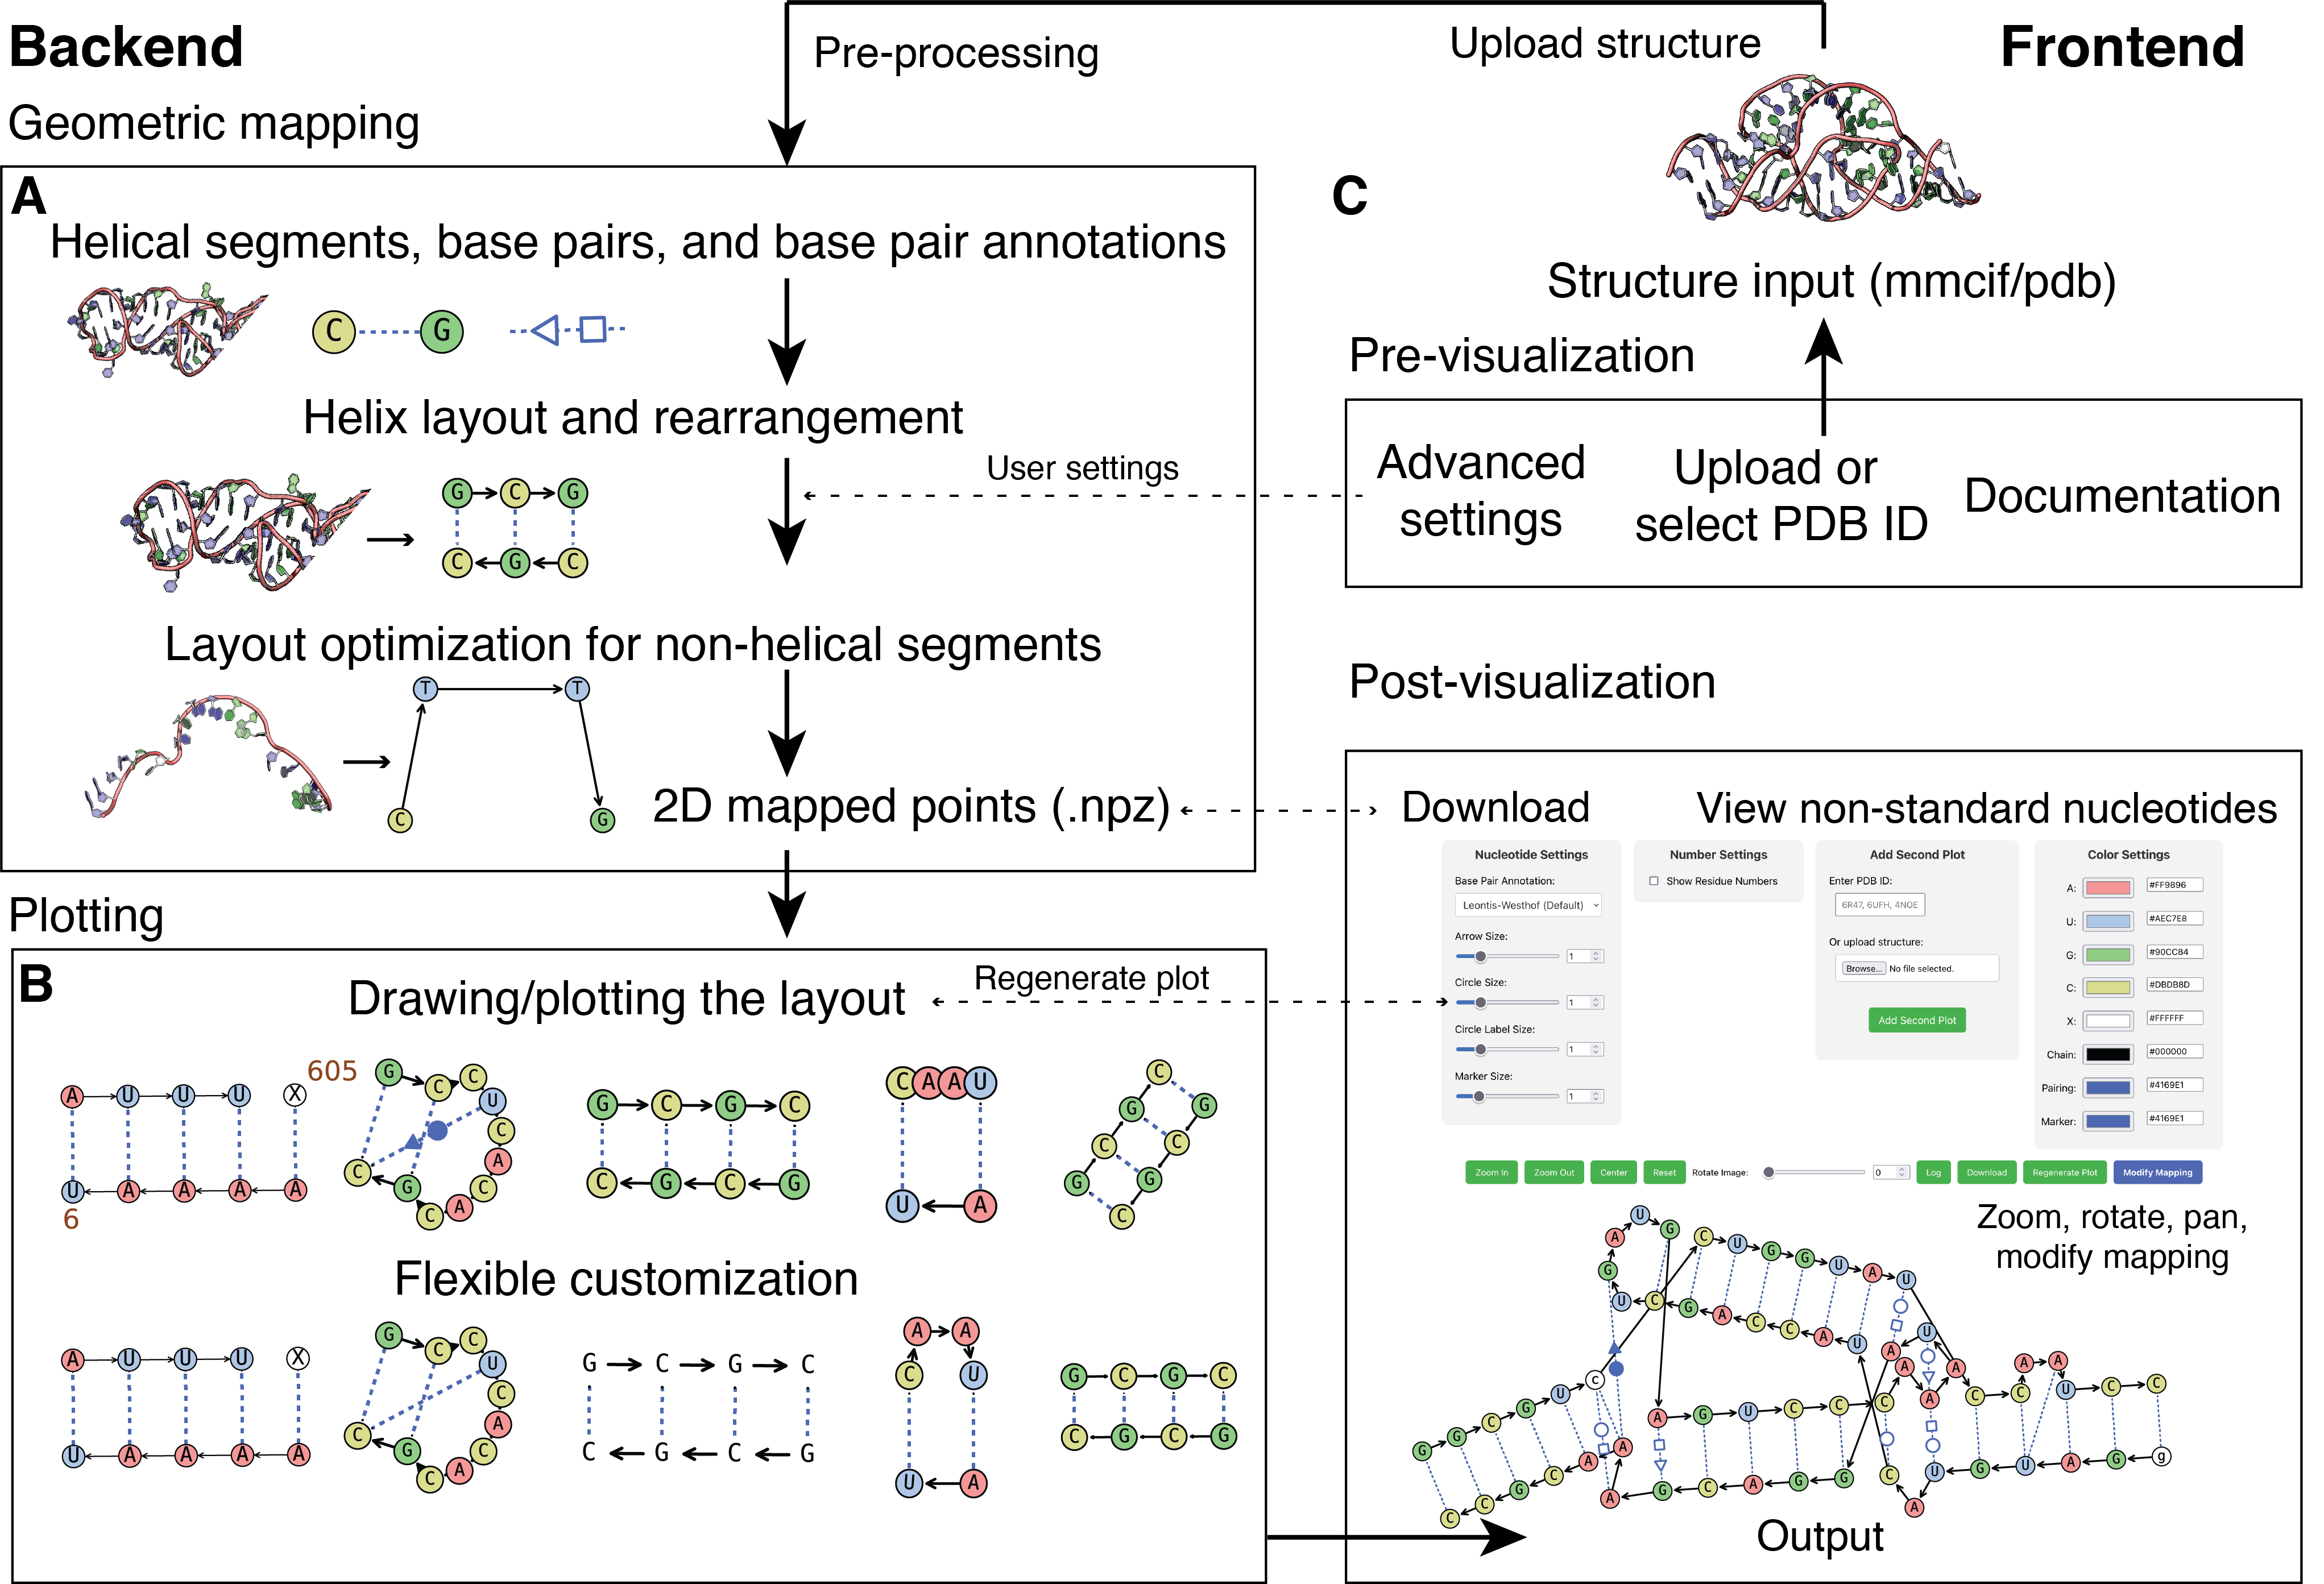
\includegraphics[width=0.8\paperwidth]{./rnascapefigs/figure2.png}}
 % archetecture.png: 1149x508 px, 72dpi, 40.53x17.92 cm, bb=0 0 1149 508
        \caption[Computational cost of training RVAgene]{\textbf{Training RVAgene is reasonably scalable on CPU and even more so using hardware acceleration through GPU.} ({\bf A}) Time cost of training RVAgene for 100 epochs for datasets with varying number of genes and time points on CPU and GPU. ({\bf B}) Maximum memory utilized during training of the model on CPU an GPU for the cases in (A), inset plot: comparison of max memory used compared to DPGP for varying number of genes.}
  \label{fig:rnascape2}
\end{figure}
\end{center}


%\section{Results}
\subsection{Application of RNAscape to structures from the PDB}

We present RNAscape output for various structures (\hyperref[fig:rnascape4]{Fig. 3.1}, \hyperref[fig:rnascape4]{3.4} from the PDB \citep{berman2000protein}). In \hyperref[fig:rnascape1]{Fig. 3.1A}, tRNA from Sulfolobus tokodaii (PDB ID: 7VNV) is shown. RNAscape output preserves the L-shaped topology (as opposed to known ‘clover leaf’ shaped secondary structure \citep{Krahn2020} visualizations) and annotates non-standard bases and base-pairing geometries (critical in many RNA interactions \citep{Hermann1999}. RNAscape can also process unusual DNA structures, as shown by a single-stranded DNA with circular topology (PDB ID: 4NOE, \hyperref[fig:rnascape1]{Fig. 3.1B}). In \hyperref[fig:rnascape1]{Fig. 3.1C}, Dengue virus RNA promoter (PDB ID: 7UMD) is depicted, which is a single-stranded RNA molecule containing only standard RNA bases.

We present a few different examples of ribozymes and riboswitches (\hyperref[fig:rnascape1]{Fig. 3.1D-G}). RNA loop modeling \citep{Sripakdeevong2011} for riboswitches is an important area of research, and RNAscape visualizations (e.g. PDB IDs: 1Y26, 4FRN, 8HBA, \hyperref[fig:rnascape1]{Fig. 3.1E-G}) may aid in these efforts. The pistol ribozyme (PDB ID: 6R47, \hyperref[fig:rnascape1]{Fig. 3.1D}) and the Nicotinamide Adenine Dinucleotide-II (NAD-II) riboswitch (PDB ID: 8HBA, \hyperref[fig:rnascape1]{Fig. 3.1G}) illustrate how RNAscape places non-helical segments and can clearly depict their non-standard base pairs with helical segments. RNAscape natively supports multiple strands (e.g. PDB ID: 1Y26, \hyperref[fig:rnascape1]{Fig. 3.1E}). RNAscape is also able to visualize G-quadruplexes (PDB ID: 2M18, \hyperref[fig:rnascape1]{Fig. 3.1H}). An RNA structural motif which can serve as a binding site for proteins is the kink-turn motif (PDB ID: 7EFG) \citep{Schroeder2010}, and it is visualized in \hyperref[fig:rnascape1]{Fig. 3.1I}.

There has been a continued interest in structural studies of the ribosome which postulate the role of a proto-ribosome \citep{Bose2022} in the origin of life. The proto-ribosome is a semi-symmetrical core of the ribosome comprised of RNA molecules representing the site for peptide bond formation, therefore known as peptidyl transferase center (PTC). The RNAscape visualization (\hyperref[fig:rnascape1]{Fig. 3.1J}, Supplementary \hyperref[fig:rnascapeS1]{Fig. S13}) for the same reflects the high degree of conformational symmetry, based on structural coordinates of the PTC provided by Bose et al. \citep{Bose2022,}.

RNAscape can run on relatively large structures (structures of up to 50 MB are processed by the webserver). In \hyperref[fig:rnascape4]{Fig. 3.4}, we demonstrate its application to four different topologies of larger structures. In \hyperref[fig:rnascape4]{Fig. 3.4A}, a triangular topology of Mycobacterium tuberculosis ileS T-box in complex with tRNA (PDB ID: 6UFH, 244 nucleotides) is shown, followed by a diamond-like topology of mutant P4-P6 domain of Tetrahymena thermophila group I intron (PDB ID: 1HR2, \hyperref[fig:rnascape4]{Fig. 3.4B}, 157 nucleotides) and an exon free state of the Tetrahymena group I intron (PDB ID: 7R6N, \hyperref[fig:rnascape4]{Fig. 3.4C}, 354 nucleotides). Secondary structure representations will not resemble the structure at all for many of these cases (e.g. stacked ladders, PDB ID: 7QDU, \hyperref[fig:rnascape4]{Fig. 3.4D}, 552 nucleotides), while RNAscape is able to reflect the 3D topology of these large RNA molecules.
\begin{center}
    \begin{figure}
    \makebox[\textwidth]{\includegraphics[width=0.8\paperwidth]{./rnascapefigs/figure3.png}}
 % archetecture.png: 1149x508 px, 72dpi, 40.53x17.92 cm, bb=0 0 1149 508
        \caption[RNAscape algorithm.]{\textbf{RNAscape algorithm.} ({\bf A})  Pre-processing of uploaded/fetched structures. Structure files are obtained either through user upload or direct download from the PDB. DSSR is run on each structure to detect helical segments and assign base-pairing annotations. ({\bf B}) Geometric mapping and post-processing of helical segments. For each helical segment, RNAscape estimates the ladder axis by connecting the centroids of the starting and ending nucleotides with a line segment. If a helix is bent, detected by a distance >10 Å between the midpoint of the ladder axis and corresponding helical segment's centroid, the ladder axis is split into two. Helical projections within 20 \AA and 30$^{\circ}$ are optionally merged. Base pairs are uniformly spaced along each ladder axis, and cramped helices are lengthened. ({\bf C}) Optimizing placement of non-helical regions followed by creation of annotated visualization. Hanging single stranded regions are mapped to their corresponding, connected helix and merged with the ladder. Loops are either preferentially bulged out in a radial curve or interpolated linearly based on a spatial density threshold. Loop direction is determined by minimizing the total nearest neighbor count of a given loop. Mapped points as well as pairing and backbone annotations are passed to the plotting script to create a visualization.}
  \label{fig:rnascape3}
\end{figure}
\end{center}
\subsection{RNAscape user interface}

The RNAscape webserver (\hyperref[fig:rnascape2]{Fig. 3.2C}) displays three primary items: header, file upload, and documentation panels. In the header, a user can click the ‘Run on Example Data’ button to view an example visualization (PDB ID: 3ZP8). In the file upload panel, a user can upload a structure using the file upload feature. This file may contain non-nucleic acid entities which will be ignored. Alternatively, a user can directly input a PDB ID to load its corresponding first assembly file. Clicking the ‘Run’ button runs the RNAscape pipeline on the uploaded structure file or provided PDB ID (biological assembly 1). After running RNAscape for a structure, a user has the option to add a second structure for side-by-side viewing. We demonstrate this capability for two structures of tRNA molecules (PDB IDs: 8UPT and 8UPY, Supplementary \hyperref[fig:rnascapeS2]{Fig. S14}), introduced by recent work \citep{Krahn2024} on the importance of tRNA shape. The documentation panel enables easy navigation and provides a quick start guide, tips, and examples for using RNAscape. It also includes detailed explanations for configurable settings.

\subsection{Output images}

The frontend (\hyperref[fig:rnascape2]{Fig. 3.2C}) natively supports touch-screen compatible image exploration. A user can zoom, center, or reset any zooming/panning via buttons above the display box. The image can also be rotated using a slider, and a ‘regenerate’ button is offered that replots the image, associated annotations, and user customizations in the desired rotation. To the right of the image, a legend is displayed that corresponds to the base-pairing annotation selected by the user. For the Saenger \citep{Saenger1984} base-pairing annotation, no legend is shown. The local strand direction ($5'$ to $3'$) is indicated by the black arrows between nucleotides for all plots. Other interactions are shown in blue dotted lines. These colors are fully customizable by the user. The user also has the option of downloading RNAscape mapped points in a numerical format (.npz) processable by the NumPy \citep{harris2020array} library. Additionally, a log is provided which contains a description of the non-standard/modified nucleotides in the plot and other associated information.

\subsection{Base-pairing annotations}

RNAscape offers three base-pairing annotation styles: LW \citep{Yang2003, Leontis2001}, DSSR \citep{lu2015dssr} and Saenger \citep{Saenger1984}. All base-pairing annotations are calculated via DSSR, although any future updates to these conventions by the nucleic acid community can be easily incorporated. Annotations do not affect geometric mapping, and a user can forego an annotation altogether. The LW annotation contains two key parameters: bond orientation (cis/trans) and base edge type. Bond orientation is represented by a filled or unfilled marker. The edge types: Watson-Crick (W), Hoogsteen (H), or sugar (S), are represented by marker shapes (\hyperref[fig:rnascape1]{Fig. 3.1}).

The DSSR style differs in that base edges are delineated by major groove (M), minor groove (m), or Watson-Crick (W) edges. Bond orientation annotation is the same as in the LW \citep{Yang2003, Leontis2001} annotation. DSSR also reports local strand orientation as a base-pairing annotation feature. RNAscape always denotes local strand orientation by the backbone arrows (\hyperref[fig:rnascape1]{Fig. 3.1}). Non-standard pairings flagged as ‘not categorized’ by DSSR are not annotated. For the Saenger \citep{Saenger1984} annotation, each bond type is represented by a number corresponding to its Roman numeral annotation.

\subsection{Customizable settings}

Several custom settings options are available (\hyperref[fig:rnascape2]{Fig. 3.2C}). The Loop Bulging setting controls whether loops are bulged outwards or linearly interpolated (see Materials and Methods). Additionally, the post-processing step of merging proximate, similarly oriented ladders can be turned off (\hyperref[fig:rnascape3]{Fig. 3.3B}). Since these settings affect the geometric mapping, a user must click ‘Run’ to run the pipeline again if they are changed. Arrow size, circle size, and circle label size affect nucleotide appearance. Base-pairing marker sizes can also be adjusted. Through the number settings, a user instructs RNAscape to label residue numbers in the numbering schema defined by the structure file. Color, size, frequency, and spacing of these labels can also be modified. Color settings allow a user to customize the color of each nucleotide type: A, C, G, U/T and X (non-standard nucleotides). Colors used to denote both backbone chain and non-chain interactions and markers can also be modified. Furthermore, RNAscape provides a functionality to modify calculated maps. By clicking on the ‘Modify Mapping’ button, the user can move and adjust nucleotide locations to resolve, for instance, overlap and regenerate the output.
\begin{center}
    \begin{figure}
    \makebox[\textwidth]{\includegraphics[width=0.7\paperwidth]{./rnascapefigs/figure4.png}}
 % archetecture.png: 1149x508 px, 72dpi, 40.53x17.92 cm, bb=0 0 1149 508
        \caption[RNAscape output for large-size structures from the PDB.]{\textbf{RNAscape output for large-size structures from the PDB.} The 3D structure at the top of each panel is from the PDB structure, with its corresponding RNAscape visualization shown below it. ({\bf A}) \textit{Mycobacterium tuberculosis} T-box in complex with tRNA (PDB ID: 6UFH, 244 nucleotides), ({\bf B}) Mutant P4-P6 domain (DELC209) of \textit{Tetrahymena thermophila} group I intron (PDB ID: 1HR2, 157 nucleotides), ({\bf C}) Exon-free state of the Tetrahymena group I intron (PDB ID: 7R6N, 354 nucleotides), and ({\bf D}) Twist-corrected RNA origami 5-helix Tile A (PDB ID: 7QDU, 552 nucleotides).}
  \label{fig:rnascape4}
\end{figure}
\end{center}

\section{Discussion}

The RNAscape webserver produces customizable, publication-quality visualizations of nucleic acid tertiary structure. It prioritizes the topology of a structure while striving to create a clean and optimized output, and it is designed to minimize user effort. RNAscape significantly deviates from any existing method in terms of its output quality, usability, and layout algorithm (\hyperref[table:rnascape]{Table 3.1}, Supplementary \hyperref[fig:rnascapeS3]{Fig. S13, S15}). Users can refine visualizations on the webserver, and RNAscape also supports non-standard nucleotides and various base-pairing annotations. Further updates to base-pairing conventions may be easily incorporated. The RNAscape webserver allows a maximum file size of 50 MB. While potentially informative, the output for extremely large structures may not be well suited for presentation. We provide the RNAscape implementation via GitHub (see Data Availability) for those inclined to try the pipeline locally on even larger structures. We conclude with the hope that our effort facilitates advancement of the ever-growing field of RNA biology

\section{Data availability}

RNAscape is freely available for all users at \url{https://rnascape.usc.edu/}. The backend implementation is also available on GitHub at \url{https://github.com/timkartar/RNAscape} and preserved through figshare at \url{https://doi.org/10.6084/m9.figshare.25201889}.
%%%%%%%%%%%%%%%%%%%%%%%%%%%%%%%%%%%%%%%%%%%%%%%%%%%%%%%%%%%%%%%%%%%%%%%%%%%%%%%%%%%%%%%%%%%%%%%%%%%%%%%%%%

%%%%%%%%%%%%%%%%%%%%%%%%%%%%%%%%%%%%%%%%%%%%%%%%%%%%%%%%%%%%%%%%%%%%%%%%%%%%%%%%%%%%%%%%%%%%%%%%%%%%%%%%%%%%%%%%%%%%%%%%%%%%%%%%%
\chapter{DNAproDB: an updated database for the automated and interactive analysis of protein–DNA complexes}
%\begin{abstract}

DNAproDB (https://dnaprodb.usc.edu/) is a widely used database, visualization tool, and processing pipeline for analyzing the structural features of protein–DNA interactions. Here we present a substantially updated version through additional data and functionalities. It contains an expanded volume of pre-analyzed protein–DNA structures, which will now be automatically updated weekly. The analysis pipeline now identifies water-mediated hydrogen bonds, and modified visualizations of protein–DNA incorporate this data. Tertiary structure-aware nucleotide layouts are now available. New file formats and external database annotations are supported. The website has been aesthetically modernized, and interactions with graphs and data is more intuitive. We also present a statistical analysis on the updated collection of structures revealing salient patterns in protein–DNA interactions.

\end{abstract}

\section{Introduction}

Protein–DNA interactions play crucial roles in essential cellular functions like gene regulation, genome packaging, and DNA replication (1, 2). Diverse recognition mechanisms underlie these interactions (3–6). Atomic resolution structures of protein–DNA complexes available in the Protein Data Bank (PDB) (7) have been invaluable for understanding these readout mechanisms and provide insight that relate them to function. As a computational resource which extensively analyzes such structures and presents their data in publication-quality representations, the DNAproDB web server (8) and database (9) have been a useful resource for biologists, recognized by tool libraries such as the Nucleic Acid Knowledge Base (NAKB) (10). 
This update improves the DNAproDB analysis pipeline, output data presentation, and web interface (Fig. 1). The updated analysis pipeline now computes annotations of water-mediated hydrogen bonds, which are known to play an important role (11) in protein–DNA recognition and, in some cases, a very prominent one (12). Also, the pipeline now automatically processes and incorporates new PDB structures weekly. The primary interface visualization, ‘Residue contact map,’ now allows users to select a mapping algorithm for nucleic acid layout. In addition to secondary structure-based mapping (13), tertiary-structure aware mapping (14) is now available. Binding specificity data for transcription factors catalogued in the JASPAR2024 (15) database has been integrated. Users can now upload structures in the macromolecular Crystallographic Information File (mmCIF) format and download interface visualizations in an editable figure format. More information regarding these updates, as well as quality-of-life and user-interface improvements, is described in the following sections.
We analyzed the expanded DNAproDB structure collection for salient features of protein–DNA interactions (Fig. 2). These results (based on a larger sample size in this update) reaffirm previous statistics presented about DNA minor groove recognition (3) and patterns of amino acid-base stacking for single stranded DNA presented (9). Additionally, we present and discuss examples of the newly added water-mediated hydrogen bond annotations in selected structures (Fig. 3).
DNAproDB has been used by experimental biologists to upload, analyze, and present interface visualizations in their work (16). We developed this update to assist their efforts, likely leading to additional contributions from the scientific community. We want to emphasize the increased utility of DNAproDB in light of structure prediction tools like AlphaFold3 (17), RoseTTAFoldNA (18), and RoseTTAFold-AA (19), and binding specificity prediction tools including DeepPBS (20) and rCLAMPS (21). These computational tools hint towards a promising future of protein–DNA structure prediction and design (22). We expect that DNAproDB will be an invaluable tool and assist such efforts.

\begin{center}
    \begin{figure}
    \makebox[\textwidth]{\includegraphics[width=0.8\paperwidth]{./dnaprodbfigs/figure1.png}}
 % archetecture.png: 1149x508 px, 72dpi, 40.53x17.92 cm, bb=0 0 1149 508
        \caption[Key aspects of this update to DNAproDB.]{\textbf{Key aspects of this update to DNAproDB.} ({\bf A}) Automatic update and separated external annotation incorporation scheme.  ({\bf B})  Different nucleic acid layout options in with added tertiary structure aware RNAscape layout, shown for PDB ID: 3LDY. ({\bf C}) Water-mediated hydrogen bond annotation. ({\bf C}) Various improvements in other aspects of DNAproDB. }
  \label{fig:dnaprodb1}
\end{figure}
\end{center}


\section{Update details}

\subsection{Processing pipeline and data update}
At the time of its previous release (9), DNAproDB contained a static collection of structures. This resulted in newly released structures being unavailable. In this update, we have addressed this limitation by implementing an automatic update pipeline (Fig. 1A). Every weekend, the pipeline queries the PDB for newly released structures, downloads and processes them, and adds them to the DNAproDB collection. 
In addition, the structure processing pipeline has been separated from any external annotation dependency. This allows external annotations to be updated without reprocessing each structure or affecting the user experience. Annotations from the JASPAR2024 (15) database (incorporating the most recent binding specificity matrix ID and logo) have been included whenever applicable. 
The asymmetric unit molecular weight cutoff, which determines whether a structure is included in the collection, has been expanded from 250 to 1500 kDa, increasing the structures available for analysis. The latest collection size as of June 7th, 2024, is 6,731 structures. This set has been analyzed and was included in the results presented in Fig. 2. 
Originally, a large part of the processing pipeline was written using Python 2 (23). However, support for Python 2 is no longer available by the open-source community as of January 1, 2020, and Python 3 (24) has become the new standard. We redesigned the backend processing pipeline to ensure compatibility with Python 3. 
As an expansion of available features, water-mediated hydrogen bonds between protein and DNA have been calculated and annotated within this update. The program HBPLUS (25), with the ‘-h’ option set to 3 Å, and the ‘-d’ option set to 3.5 Å, and with the remaining parameters set as default, is used to detect hydrogen bonds. Custom scripts were written to determine water-mediated interactions via shared water molecules between hydrogen-bonded pairs (see Data Availability).  

\subsection{Visualization}
We updated the ‘Residue contact map’ and ‘3D structure’ (Fig. 1B) visualizations presented in DNAproDB in several ways. The nucleic acid backbone color used in these components has been changed to a more visually pleasing metallic blue-gray color, compared to the previously used yellow-orange color. 
In addition to the previous secondary-structure-based and circular layouts, an RNAscape (14) based layout for placing nucleic acids has been computed and added to the ‘Residue contact map’. This new layout is more representative of tertiary structure compared to the other two representations (Fig. 1B). An option to switch between these different layouts is available.
During this update, some Python 2 version utilities for secondary structure-based layout computation were discontinued. We replaced these utilities with analogous Python 3 versions provided by the ‘Forgi’ (26) package. 
Water-mediated hydrogen bonds have now been incorporated as an interaction edge in the ‘Residue contact map’. These are indicated by a black circle (Fig. 1C) in the interaction map. Hovering over the water-mediated contacts will present further information (e.g., residue number of the water molecule involved). An option to hide these interactions is also available. The ‘3D structure’ component now displays the solvent alongside the structure (in a previous version, the solvent was removed). A button to hide solvent is included. 

\subsection{Web interface and user experience}

Since its inception, we have continuously provided support for DNAproDB users and taken note of their feedback. In this update, we redesigned the web interface based on this information (Fig. 1D). Textual clutter has been reduced on the home page and report pages for each structure. Instructions and explanations for different components, which were previously written directly on the page, are now available as pop-up components upon mouse hover. Report pages for each PDB entry now prominently display the title of the entry. The information tables have been rearranged in a modern and tabular fashion, resulting in further decluttering of information. 
DNAproDB offers many customization features for the Residue contact map. However, these options were often overlooked by users due to their non-prominent placement on the website. We have redesigned the user interface to make basic options like rotation, zooming, download, and switching between the layout algorithms easily accessible directly above the visualization. Buttons to access further customization options (‘Chart options’ and ‘Interface selection’) are prominently placed. The options within the ‘Chart options’ tab have been expanded. Within the ‘Interface selection’ tab, basic options (model, entity, chain, moiety selection) are shown first. Additional options are presented as advanced options. Mouse-based interaction controls for the ‘3D viewer’ and ‘Residue contact map’ have been made analogous, as much as possible.
The download option now supports the editable Scalable Vector Graphics (SVG) format. DNAproDB currently displays Watson-Crick, Hoogsteen, and other base-pairing geometries via correspondingly stylized base-pairing edges (e.g., Hoogsteen base-pairing in p53-tetramer-DNA complex (5) reflected in Fig. 3E). For additional analysis of non-Watson-Crick base-pairing geometries, a link to the RNAscape (14) webserver has been included in each report page. Clicking this link will redirect the user to the RNAscape website and automatically run it on the desired structure.

\subsection{Quantitative analysis of readout features}
Entries in the DNAproDB collection (as of June 7th, 2024) encompass protein–DNA structures including single-stranded (ssDNA), double-stranded DNA (dsDNA), and other conformations (e.g., G-quadruplex). We quantified the growth of such entries over time based on their PDB release dates, which reflects an exponential trend (Fig. 2A). Fewer entries contain ssDNA and other conformations compared to dsDNA. However, recent years (2016 onwards) demonstrate a steady growth also in ssDNA entries (Fig. 2A). 
Studies on protein-DNA structures have revealed consistent patterns in protein residue–DNA interaction frequencies (3, 27). We sought to quantify similar statistics in the updated collection of DNAproDB. To this end, we computed relative abundances of different amino acids interacting with the major groove (Fig. 2B), minor groove (Fig. 2C), and phosphodiester backbone (Fig. 2D). Relative abundance for a residue (R) is the fraction of appearance of this protein residue in an interaction with a DNA moiety relative to other residues. 
Relative abundance (R) = |interactions involving R|R|interactions involving R|

\begin{center}
    \begin{figure}
    \makebox[\textwidth]{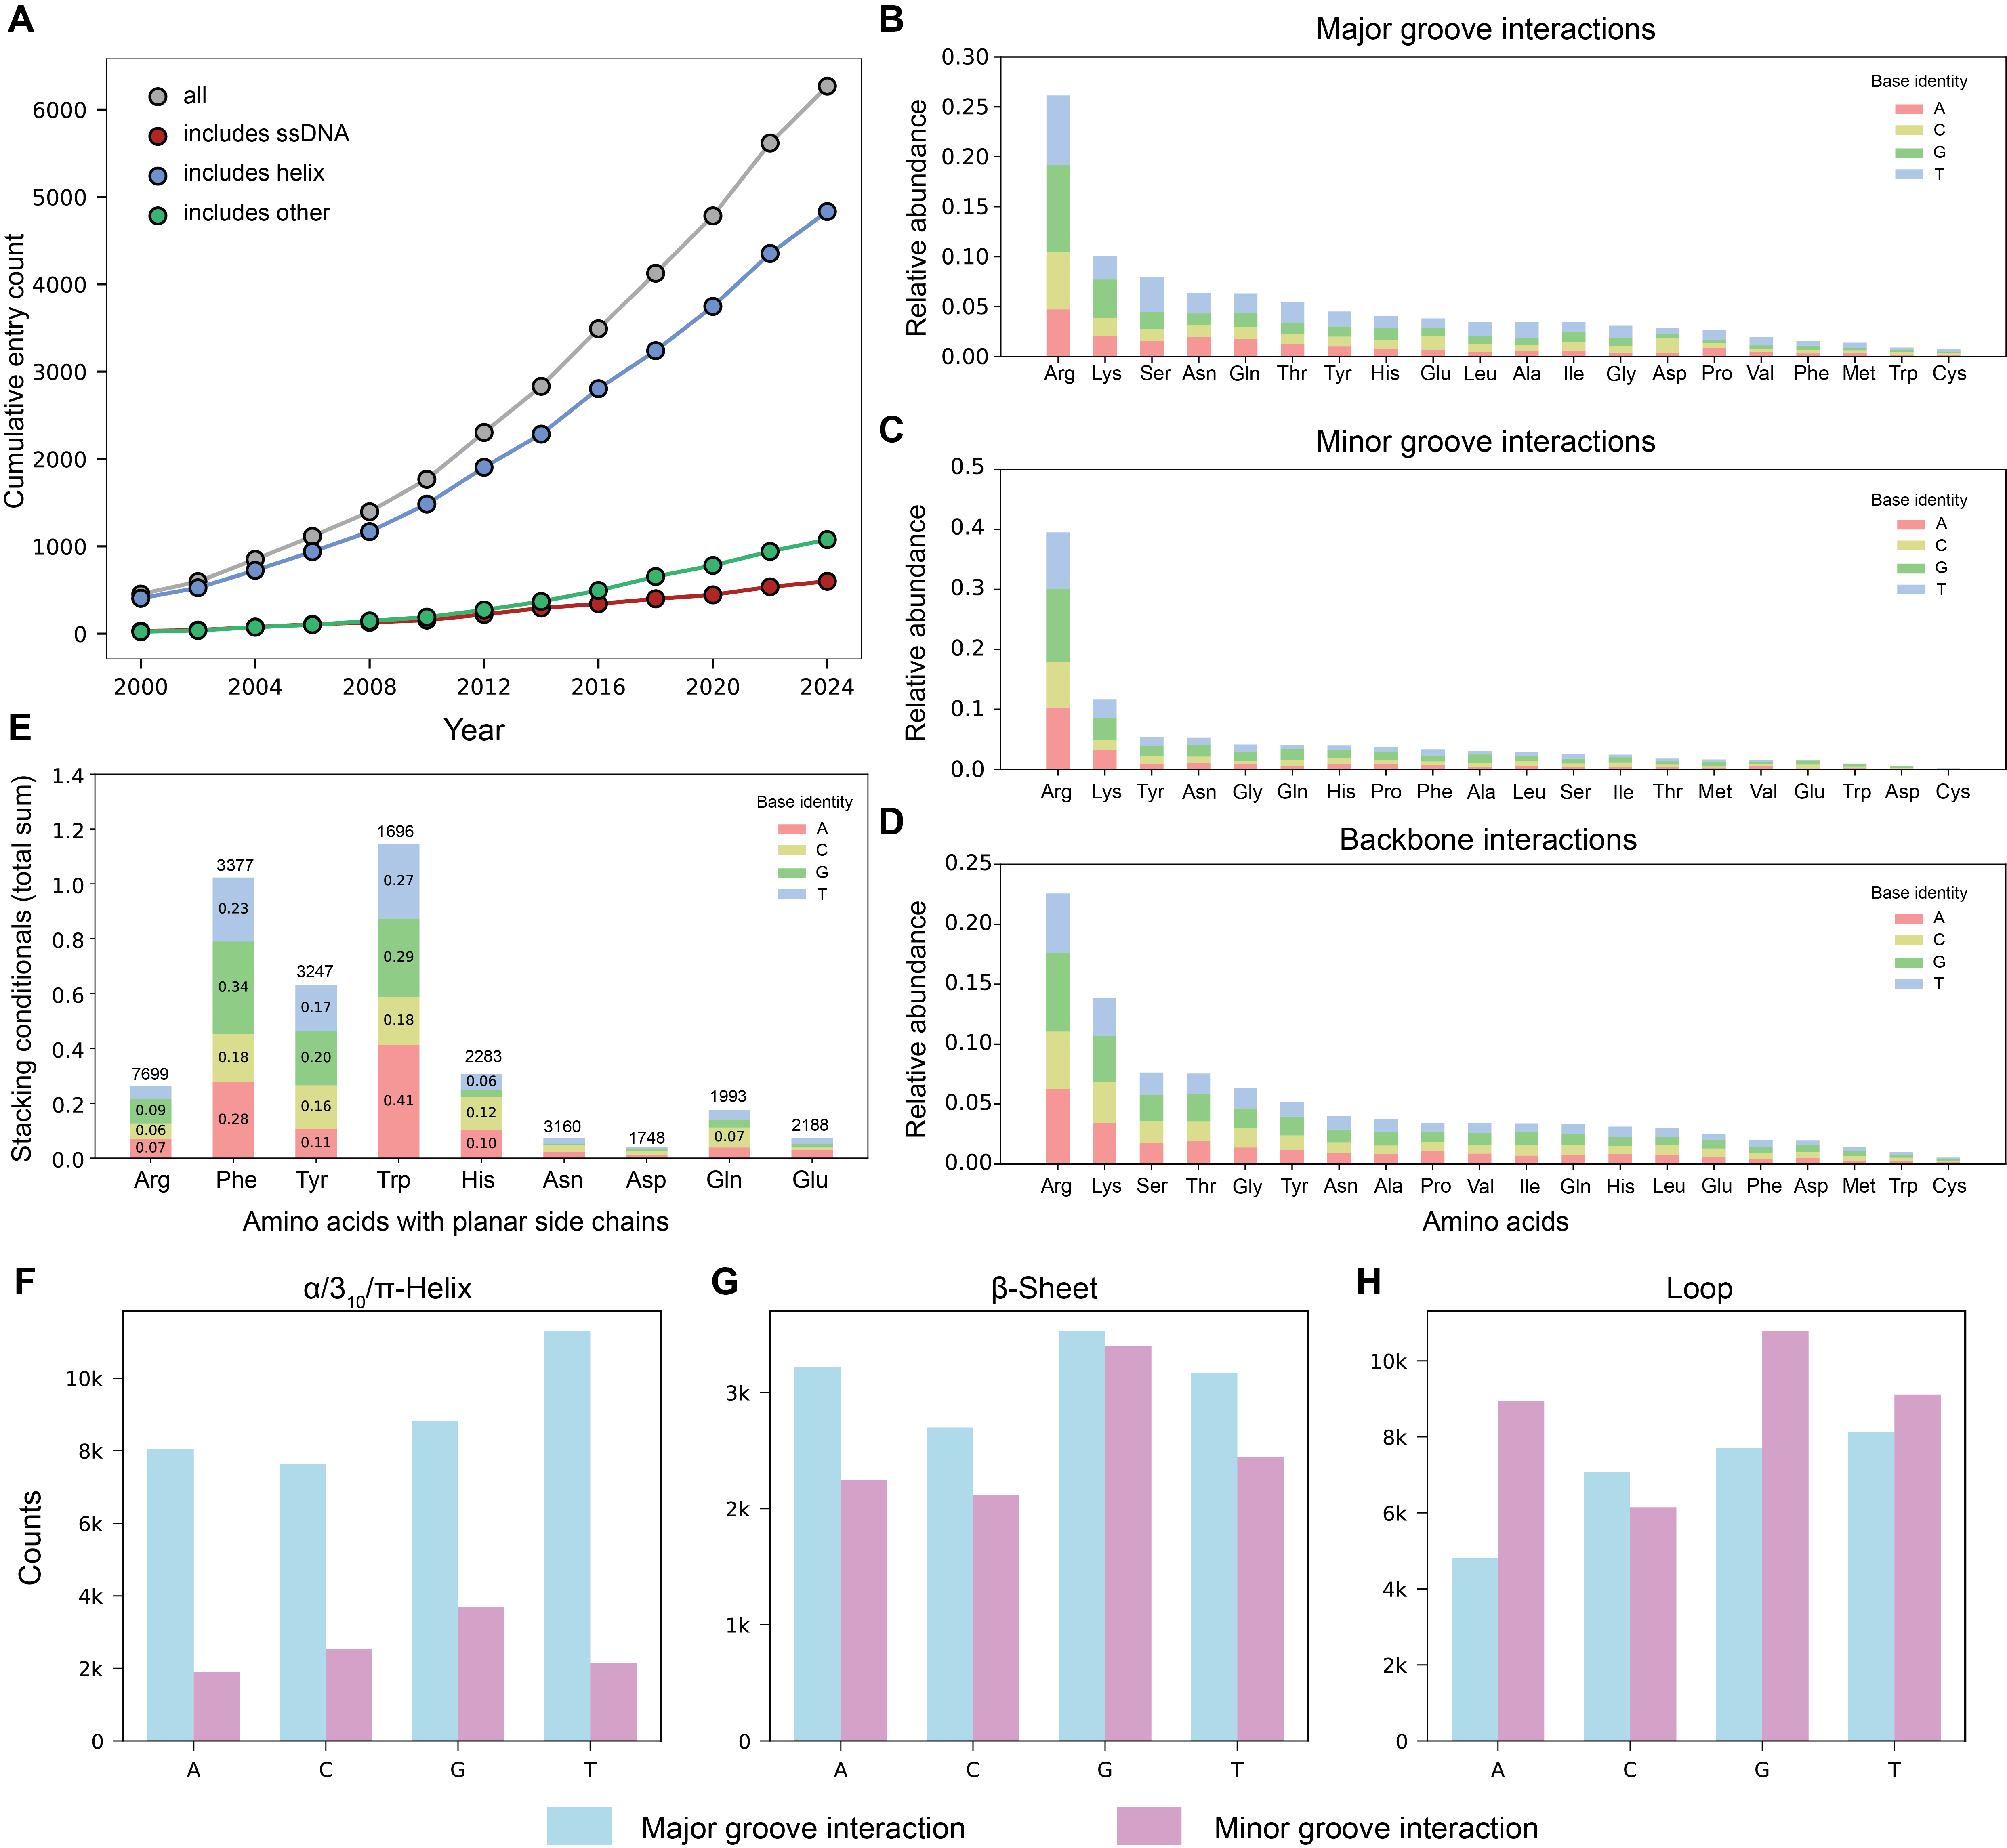
\includegraphics[width=0.8\paperwidth]{./dnaprodbfigs/figure2.png}}
 % archetecture.png: 1149x508 px, 72dpi, 40.53x17.92 cm, bb=0 0 1149 508
        \caption[Quantitative analysis of protein–DNA complexes in the DNAproDB collection. ]{\textbf{Quantitative analysis of protein–DNA complexes in the DNAproDB collection. } ({\bf A}) PDB release years of structures catalogued in the updated DNAproDB collection (as of June 7th, 2024). ({\bf B-D})   Relative abundance of different amino acids interacting with DNA major groove (B), minor groove (C), and phosphodiester backbone (D). ({\bf E}) Conditional probabilities of different protein residues and base forming a stacking geometry. Y-axis represents summed values over the bases for each amino acid.({\bf F-H}) Counts of interactions with different bases, categorized by major and minor groove for secondary structure classes: Helix (includes $\alpha$/$3_{10}$/$\pi$-helix) (F), Sheet ($\beta$-sheet) (G) and loop residues (H) }
  \label{fig:dnaprodb2}
\end{figure}
\end{center}

This is computed separately for the major groove, minor groove, and DNA backbone. Each of these values in Fig. 2B-E is further subdivided into fractions per DNA base, shown in four colors. For the major groove, we see an abundance of residues able to perform recognition via hydrogen bonds with arginine (Arg) and lysine (Lys) residues showing the greatest presence (Fig. 2B). For the minor groove, this preference for arginine and lysine is even stronger relative to other residues (Fig. 2C). This agrees with the observation that the minor groove is more electronegative (3), favoring positively charged amino acid sidechains while repelling negatively charged sidechains (e.g., aspartic acid (Asp), glutamic acid (Glu) etc.). 
For amino acid residues (R) with a planar side chain component (i.e., able to form a stacking interaction with a base (B $\in$ [A,C,G,T]) in single-stranded DNA), interaction geometries (g) can be of three types: g $\in$ [stack, pseudo pair, other]. Stacking conditionals P(g=stack | R, B) were computed for major and minor groove interactions as a fraction of the counts of stack geometry against counts for all geometries. i.e.,
P(g=stack | R, B)= |g=stack, R,B|  g|g, R, B| 
This information is presented in Fig. 2E in the form of a stacked bar chart. The total height of each stacked bar (i.e., for each amino acid) is BP(g=stack | R, B) . The pattern visible in this data conforms with the previously computed version in (9) while encompassing a larger sample size.
DNAproDB also provides annotations and a visualization (‘Helical contact map’) reflecting how various secondary structure elements of a protein interact with the major and minor groove of DNA. We quantified these interactions to reveal statistical patterns (Fig. 2F-H). We compute instances of helical secondary structures (including -helices, -helices, and 310-helices) interacting with the four primary DNA bases in either the major or minor groove (Fig. 2F). There is a clear preference for the major groove for protein helices, reflecting the use of a recognition helix by many protein families (28). On the other hand, for -sheets, major and minor groove interactions are comparable in number, with a slight preference for the major groove (Fig. 2G). The ‘loop’ category reflects residues appearing in loop regions of proteins interacting with DNA. Minor groove interactions are slightly more favored in this case (Fig. 2H). In all cases, guanine (G) is the most favored DNA base that is contacted. 

\subsection{Water-mediated hydrogen bonds}
As described previously, the updated DNAproDB processing pipeline detects and visually annotates (Fig. 1B) water-mediated hydrogen bond interactions between protein and DNA. This feature improves the accuracy and relevance of the DNAproDB visualization for some structures. For example, the co-crystal structure of the Trp repressor/operator complex (PDB ID: 1TRO, Fig. 3A, Residue contact map: Fig. 3B) reflects a protein–DNA recognition scheme without any direct hydrogen bonds in the major and minor groove. Instead, DNA recognition occurs via water-mediated hydrogen bonds (Fig. 3B) (12). A detailed view of two protein backbone nitrogen atoms (belonging to Ile79 and Ala80) recognizing G11 in this manner is presented in Fig. 3C. This type of recognition scheme was previously not reflected in DNAproDB. Similarly, protein residues interacting with DNA only through water-mediated hydrogen bonds were also not displayed in the Residue contact map. One such example is the p53 tetramer structure (PDB ID: 3KZ8 (5), Fig. 3D, Residue contact map: Fig. 3E). This structure illustrates serine residues (Ser121) near the tetramerization interfaces involved in water-mediated hydrogen bonds with the major groove edge of two G bases (shown for one selected base in Fig. 3F). As this is the sole mode of interaction for these two residues, they were omitted from the visualization in the previous DNAproDB version (9). In this update, these interactions are correctly shown. A variety of complex interaction geometries are possible when water-mediated hydrogen bonds are involved. One such example can be found in interactions of the RXR/RAR DNA-binding domain heterodimer in complex with the retinoic acid response element (PDB ID: 1DSZ (29), Fig. 3G, Residue contact map: Fig. 3H). The lysine residue (Lys1260) is involved in recognizing consecutive bases (G and T) through water-mediated hydrogen bonds involving two different water molecules. This update to DNAproDB allows exploring such recognition schemes. 

\begin{center}
    \begin{figure}
    \makebox[\textwidth]{\includegraphics[width=0.8\paperwidth]{./dnaprodbfigs/figure3.png}}
 % archetecture.png: 1149x508 px, 72dpi, 40.53x17.92 cm, bb=0 0 1149 508
        \caption[Water-mediated hydrogen bond annotation in DNAproDB]{\textbf{Selected examples of water-mediated hydrogen bond annotations as reflected in the updated DNAproDB.  } ({\bf A-C}) Trp repressor/operator complex (PDB ID: 1TRO)  ({\bf D-F})    p53 tetramer with Hoogsteen base pairs (PDB ID: 3KZ8). ({\bf G-I}) Conditional probabilities of different protein residues and base forming a stacking geometry. Y-axis represents summed values over the bases for each amino acid.({\bf F-H}) RXR-RAR DNA-binding complex (PDB ID: 1DSZ). In each of the three cases, the 3D structure of the respective complex is shown in (A, D, G). The DNAproDB Residue contact map is shown (with only selected protein residues annotated) in (B, E, H). Atomic views of selected water-mediated hydrogen bond interactions are shown in (C, F, I), respectively. }
  \label{fig:dnaprodb3}
\end{figure}
\end{center}


\section{Discussion}
DNAproDB, since its inception in 2017 (8), has been a valuable resource for the structural biology community. Its unique and extensive analysis pipeline, covering diverse aspects of protein–DNA binding, outputs data that can be readily used in downstream analysis by the user (9). The interactive and publication-quality visualizations presented by DNAproDB have been used extensively by the structural biology community. In this update, we improved DNAproDB in multiple aspects. New structures released since the last update in 2019 (9) have been incorporated, resulting in a much larger collection. The pipeline has been future-proofed via the new automatic update feature. The backend implementation has been upgraded to Python 3, ensuring a long-lasting lifespan for DNAproDB. 
A key scientific improvement in the analysis pipeline is the incorporation of water-mediated hydrogen bond calculation. Interest in water-mediated interactions has been growing. This is evidenced by the CASP16 challenge for predicting solvent shells around the Tetrahymena ribozyme structure (30). Currently, these interactions are not well modelled by structure prediction and analysis tools (17–20, 31, 32). We expect that this added feature in DNAproDB advances the field in the understanding of readout mechanisms. 
Visualizations have been improved by enabling tertiary structure-aware nucleic acid layouts, incorporation of water-mediated hydrogen bond indicators, greater customizability, and other aesthetic changes. The website style has been redesigned, and data presentation has been improved. Structure files in mmCIF format can now be uploaded, which was previously unsupported. Altogether, these updates result in an updated DNAproDB, which we expect to continue serving the structural biology community for the foreseeable future.

\subsection{Data availability}
DNAproDB is freely available for all users at \url{https://dnaprosb.usc.edu/}. The previous version remains available at \url{https://dnaprosb.usc.edu/v1/}. 
The pipeline and frontend implementations are available via GitHub:
\url{https://github.com/timkartar/DNAproDB}; 
\url{https://github.com/ariscohen/DNAproDB_frontend}

%\section{Introduction} 

The structural diversity of RNA molecules influences their broad biological functions \citep{Tomezsko2020, seemann2017identification, Mortimer2014}. This diversity \citep{Batey1999} is primarily driven by its ability to form complicated tertiary interactions, a plethora of non-standard base-pairing conformations and quaternary interactions with other RNA, DNA or protein molecules. Visualizing RNA in two dimensions poses the challenge of capturing these complex interactions while remaining comprehensible and valuable to researchers.
\par
One popular means of representing complicated RNA structures is through secondary structure diagrams. These two-dimensional (2D) diagrams are exclusively driven by base-pairing relationships and laid out in an abstract space. Extensive literature and software \citep{Johnson2023, Sweeney2021,Weinberg2011,Wiegreffe2019,Shabash2019,Peter2003,Byun2009,Darty2009,Kerpedjiev2015,Lu2018,Waterman1978} describe secondary structure diagrams. However, these representations do not effectively capture tertiary molecular interactions, such as base pairing, stacking, and pseudoknot interactions. Therefore, although this approach scales relatively well for large RNA sequences \citep{Johnson2023}, not considering tertiary interactions can lead to a diagram far from the biological structure and function. More specifically, nucleotides which are positioned relatively close together in three-dimensional (3D) space may appear far away in the visualization.
\par
Some tools promise to capture tertiary interactions \citep{Yang2003,Mallet2022}. Of these tools, RNAView \citep{Yang2003}, is widely known and has been a current standard linked in the Nucleic Acid Knowledge Base (NAKB) \citep{Lawson2024}. However, RNAView \citep{Yang2003} lacks a webserver, requires a complicated setup and usage pipeline, and cannot handle some complex topologies resulting in output that is not always interpretable or intuitive. Moreover, it is unable to provide publication-quality images. The only other available tool that retains tertiary interactions, RNAglib \citep{Mallet2022}, is not deterministic and results in different outputs for repeat runs under the default configuration documented by the authors, which likely explains why it has not been adopted by the field compared to RNAView. A description of different tools which create various 2D diagrams of RNA molecules is provided in \hyperref[table:rnascape]{Table 3.1}.
\par
RNAscape addresses and overcomes the outlined issues and limitations of existing approaches at several levels. The RNAscape algorithm includes a mapping process that conforms to the helical geometry of RNA structures. By doing so, it attempts to preserve the intuitive correspondence between the 2D mapping and 3D structure. At the same time, RNAscape optimizes each layout to place non-helical segments of the structure without sacrificing tertiary interactions. This enables visualizations that are compact while remaining as visually intuitive as possible (Figure 1, Supplementary Figures S1 and S3).
RNAscape output for various structures from the PDB. The 3D structure at the top of each panel is from the PDB structure, with its corresponding RNAscape visualization shown below it. (A) tRNA from Sulfolobus tokodaii (PDB ID: 7VNV), (B) a single-stranded DNA molecule (PDB ID: 4NOE), (C) Dengue virus RNA promoter (PDB ID: 7UMD), (D) Pistol ribozyme (PDB ID: 6R47), (E) Riboswitch from Escherichia coli (PDB ID: 1Y26), (F) Cobalamin riboswitch regulatory element (PDB ID: 4FRN), (G) NAD-II riboswitch (PDB ID: 8HBA), (H) G-quadruplex (PDB ID: 2M18), (I) RNA kink-turn motif (PDB ID: 7EFG) and (J) the semi-symmetric peptidyl transferase center (PTC) of the large ribosomal subunit of Deinococcus radiodurans (PDB ID: 1NKW), also known as proto-ribosome (30). The molecular structure in (J) is shown along the two-fold pseudo-symmetry axis, with an additional orientation shown in Supplementary Figure S1.
\par
The RNAscape webserver (Figure 2) offers various customization options for its visualizations. Users can zoom, pan, and rotate images directly on the webserver. In addition, one can easily customize a plot with different base-pairing annotations \citep{Yang2003, Saenger1984,lu2015dssr}, residue colors, nucleotide or text-label sizes, and numbering schemas. RNAscape encourages users to iteratively refine an image. In addition, RNAscape allows the user to modify the calculated map. Upon completion, RNAscape visualizations can be exported to vector format (SVG) or image format (PNG), enabling further refinements by the user. Both Protein Data Bank (PDB) and macromolecular Crystallographic Information File (mmCIF) format files are supported to maximize compatibility. Additionally, RNAscape can directly fetch structures (biological assembly 1) from the PDB \citep{berman2000protein,} based on a given PDB ID. RNAscape supports multiple base-pairing annotation conventions: Leontis-Westhof (LW) \citep{Yang2003}, Saenger \citep{Saenger1984}, DSSR (Dissecting the Spatial Structure of RNA) \citep{lu2015dssr} and a no-annotation option. Future updates to base-pairing conventions by the nucleic acid community can easily be incorporated. Modified/non-standard nucleotides are denoted by a white circle and annotated with a small letter code (based on its parent standard base or simply ‘x’ if this information is unavailable).
\begin{center}
    \begin{figure}
    \makebox[\textwidth]{\includegraphics[width=0.8\paperwidth]{./rnascapefigs/figure1.png}}
 % archetecture.png: 1149x508 px, 72dpi, 40.53x17.92 cm, bb=0 0 1149 508
        \caption[RNAscape output for various structures from the PDB.]{\textbf{RNAscape output for various structures from the PDB.} The 3D structure at the top of each panel is from the PDB structure, with its corresponding RNAscape visualization shown below it. ({\bf A}) tRNA from Sulfolobus tokodaii (PDB ID: 7VNV), ({\bf B}) a single-stranded DNA molecule (PDB ID: 4NOE), ({\bf C}) Dengue virus RNA promoter (PDB ID: 7UMD), ({\bf D}) Pistol ribozyme (PDB ID: 6R47), ({\bf E}) Riboswitch from Escherichia coli (PDB ID: 1Y26), ({\bf F}) Cobalamin riboswitch regulatory element (PDB ID: 4FRN), ({\bf G}) NAD-II riboswitch (PDB ID: 8HBA), ({\bf H}) G-quadruplex (PDB ID: 2M18), ({\bf I}) RNA kink-turn motif (PDB ID: 7EFG) and ({\bf J}) the semi-symmetric peptidyl transferase center (PTC) of the large ribosomal subunit of Deinococcus radiodurans (PDB ID: 1NKW), also known as proto-ribosome (30). The molecular structure in (J) is shown along the two-fold pseudo-symmetry axis.}
  \label{fig:rnascape1}
\end{figure}
\end{center}

%% Please add the following required packages to your document preamble:
% \usepackage{graphicx}
\begin{table}[]
\label{table:rnascape}
\resizebox{\textwidth}{!}{%
\begin{tabular}{lllllll}
Method & Preserves 3D topology & Input & Webserver & Upload limit & Output & Framework needed \\
RNAscape \citep{Mitra2024rnascape} & Yes & .pdb, .cif & Yes & 50 MB & .png, .svg, .npz & Python (dependencies installed via pip) \\
RNAview \citep{Yang2003}  & Yes & .pdb, .cif & No & N/A & .ps & C, make based installation \\
RNAglib \citep{Mallet2022} & Semi (2.5D graphs) & .cif, compiled dataset by authors & No & N/A & .png, .svg & Python (dependencies installed via pip) \\
RNAcanvas \citep{Johnson2023} & No (secondary structure) & dot-bracket/ss formats & Yes & N/A & .svg, .pptx, interactive GUI & Unavailable \\
Forna \citep{Kerpedjiev2015}  & No (secondary structure, force directed) & dot-bracket, .pdb, .cif, .json & Yes & 2 MB & .png, .svg, .json, interactive   GUI & JavaScript \\
VARNA \citep{Darty2009} & No (secondary structure) & dot-bracket/ss formats & No & N/A & .eps, .svg, .xfig, .jpg, .png & Java \\
jVizRNA \citep{Shabash2019} & No (spring based) & dot-bracket/ss formats & No & N/A & interactive GUI & Java \\
PseudoViewer \citep{Byun2009} & No (but considers pseudoknots) & dot-bracket/ss formats & Yes & N/A & .eps, .svg, .gif, .png, bracket   view & Microsoft .NET Framework \\
XRNA (link) & No (secondary structure) & special program specific format & No & N/A & .ps & Java \\
RNAViz \citep{Peter2003} & No (secondary structure) & dot-bracket/ss formats, DCSE   alignment & No & N/A & image format (exact unknown) & C, make based installation \\
RNAPuzzler \citep{Wiegreffe2019} & No (secondary structure) & dot-bracket/ss format (.txt) & No & N/A & image format (exact unknown) & C, make based installation \\
R2R \citep{Weinberg2011} & No (secondary structure) & Stockholm format (alignment) & No & N/A & .pdf, .svg & command line program for UNIX   like systems \\
R2DT \citep{Sweeney2021} & No (predicted secondary   structure) & RNA sequence & Yes & N/A & .txt, .svg & command line tool with   Docker/Singularity \\
RNArtist (link) & No (secondary structure) & dot-bracket/ss formats, .pdb & No & N/A & .svg & Java (jdeploy) \\
Ribosketch \citep{Lu2018} & No (secondary structure, force   directed) & dot-bracket/ss formats & Yes & N/A & .txt, .svg, interactive GUI & standalone installer \\
RNAvista \citep{antczak2019rnavista} & No (prediction tool for secondary/tertiary   structure) & FASTA or dot-bracket/ss formats & Yes & N/A & .svg, predicted 3D model (.pdb) & unavailable
\end{tabular}%
}
\caption[escription of various attributes of relevant tools which produce 2D
visualizations of RNA.]{The first row corresponds to RNAscape. The next two rows correspond to two
methods which incorporate tertiary interactions in their output mapping: RNAView \citep{Yang2003} being the most
frequently used, and RNAglib \citep{Mallet2022} being the most recent. The remaining rows indicate secondary
structure drawing tools: Forna \citep{Kerpedjiev2015} being the most used (supports structure upload) and RNAcanvas \citep{Johnson2023} being the most recent (does not support structure upload). Abbreviations used: ss (secondary
structure); GUI: Graphical User Interface; Dot-bracket: RNA sequence and secondary structure in dot-
bracket format.}
\end{table}

\section{Materials and methods} 

\subsection{Programming languages and general tools}

The RNAscape webserver is a single-page web application. The backend \hyperref[fig:rnascape2]{(Figure 2A, B)} is implemented in Python 3.9.18, and Django \citep{Django2019} is used to communicate with the backend. The frontend is \hyperref[fig:rnascape2]{(Figure 2C)} designed in React v18.2.0 framework and implemented in Hypertext Markup Language (HTML)/Cascading Style Sheets (CSS)/JavaScript.

\subsection{The RNAscape algorithm}

Upon upload, the structure file is sent via Hypertext Transfer Protocol Secure (HTTPS) to the RNAscape webserver where backend processing occurs. If a user selects a PDB ID \citep{berman2000protein}, its corresponding first biological assembly is downloaded by the backend \hyperref[fig:rnascape2]{(Figure 2A, B)} for processing.

\textit{Pre-processing} \hyperref[fig:rnascape3]{(Figure 3A)}. The DSSR program (v1.7.8) \citep{lu2015dssr} is run on the structure file to detect helices and base pairs, and assign base-pairing annotations.

\textit{Helical regions} \hyperref[fig:rnascape3]{(Figure 3B)}. The positioning of helices, as well as non-helical regions, involves multiple considerations. The 3D coordinates of each nucleotide are represented by the centroid of atoms belonging to it (i.e. for the $i^{th}$ nucleotide, $V_i  = \frac{1}{|atoms(i)|}\sum\limits_{a\in atoms(i)}[a_x,a_y,a_z]$
). The set of all nucleotide centroids is a combination of two subsets (i.e. 
$V = V_H \cup V_{NH}, V_H$ (helical regions) and $V_{NH}$ (non-helical regions)). Helical regions receive the highest priority and are placed in a way that reflects their spatial orientation while remaining visually intuitive. To do so, first, we run principal component analysis (PCA) exclusively on the helical segments ($V_H$) and project the points onto the plane determined by the first two components. In this process, the $|V_H|\times 3$ sized matrix $V_H$ is converted to a $|V_H|\times 2$ matrix (which we can denote as $T$), which preserves the maximum spatial variance possible in two dimensions \citep{Pearson1901}. Next, we convert $T$ into a more visually intuitive ‘ladder’ representation, which first involves estimating a ladder axis in the projection plane for each helix. An initial estimate is made by connecting the centroid of the first and last base pairs of a helical region using a line segment. $T$ consists of multiple helical regions (i.e. $T=T_{H1}\cup T_{H2}\cup ... \cup t_{Hn}$). If the midpoint of a base-pair $B \in T_{Hk}$ is $T_{Hk}^{B}$
, the ladder axis for $T_{Hk}$ is the vector $L_{Hk} = T_{Hk}^{B_{last}} - T_{Hk}^{B_{first}}$, rooted at the point $T_{Hk}^{B_{first}}$.


However, for bent helices, this estimate may be imprecise. To account for this case, we measure the distance
 between the centroid of the helical projection and the midpoint of the estimated ladder axis (i.e. $d = |centroid(T_{Hk}) - (T_{Hk}^{B_{first}} + \frac{1}{2}L_{H_k})|$
. If this distance is greater than 10 \AA, we re-estimate the ladder axis as a combination of two line segments: one connecting the first and central base-pair centroids and another between the central and last base-pair centroids. In theory, this process can be recursively performed. In practice, however, we observe that doing so once suffices. Next, if two helical projections are within a certain distance threshold (i.e. $T_{Hk}^{B_{first}} - T_{Hk+1}^{B_{last} < 20 \AA}$
Å) and have similar orientations (i.e. 
$cos^{-1}$ 
($\frac{L_{Hk}}{|L_{Hk}|}$ 
$.$ 
$\frac{L_{H{k+1}}}{|L_{H{k+1}}|})$ 
$<$ 
$\frac{\pi}{6}$
), we merge them and recompute the ladder axis as described above. Next, we uniformly distribute the base pairs in the ‘ladder’ formation along each ladder axis. Finally, for cases where the projection of a helix is skewed, resulting in an overly cramped ladder representation, we lengthen the ladder to reduce visual clutter. The final mapping for nucleotide points in helical regions can be denoted as $P_H$.
\textit{Non-helical regions} \hyperref[fig:rnascape3]{(Figure 3C)}. Loops are either preferentially bulged out in a radial curve or interpolated linearly based on a spatial density threshold (see implementation in Data Availability), depending on the chosen setting. We choose bulging by default to reduce graph overlap and crowding. For bulging out, the structure mapping algorithm computes potential layouts and performs greedy optimization to select an optimal layout. This optimization considers the total nearest-neighbor count (within 10 \AA) of all members of a loop, and the orientation with the lowest number of neighbors is selected. Let us assume that the loop is connected to two nucleotides which are part of a helical region, mapped to positions $P_H^i, P_H^j \in P_H$ . Two possible circular layouts are computed for the loop based on $P_H^i, P_H^j$: bulging out in perpendicular directions $P_H^i - P_H^j\times \vec{Z}$
(layout $L_{pos}$) and $-(P_H^i - P_H^j\times \vec{Z})$ 
(layout $L_{neg}$), where $\vec{Z}$
denotes the unit vector which is perpendicular relative to the mapping plane. In each case, the center of the layout remains at the point $(P_H^i + P_H^j)/2$
. The radius of the circular arc is either $|(P_H^i - P_H^j)/2|$ or $|\sqrt{n}\times(P_H^i - P_H^j)/2|$
, if $|(P_H^i - P_H^j)| < 3 \AA$ or $|(P_H^i - P_H^j)/n| < 1.5 \AA$
where $n$ is the number of points in the loop. Points are uniformly distributed on the circular arc. One of the two loop orientations is selected based on minimizing the neighbor count in helical segments as follows:
\begin{align}
{argmin}_{L\in{L_{pos},L_{neg}}}\sum\limits_{p\in L}\sum\limits_{v\in P_H}\bI[|v-p| < 5 \AA]
\end{align}

Hanging single stranded regions are linearly interpolated based on its connecting mapped helix. Additional adjustments are made for certain edge cases, such as, when a linearly interpolated non-helix nucleotide exactly overlaps with another nucleotide (see implementation in Data Availability). Structures containing no helices (generally rare) are mapped solely using a PCA.

Visualization  \hyperref[fig:rnascape3]{(Figure 3C)}. The RNAscape backend utilizes the Matplotlib \citep{Hunter2007,} and NetworkX \citep{Hagberg2008} packages to plot visualizations. As input, the plotting algorithm requires the mapped points, base-pairing annotations, and user-selected visual settings for a structure. As output, it generates an image that is temporarily stored (up to 48 h) on the webserver and tied to a specific user session. Structure files are not stored. The image is served to the frontend via a Django \citep{Django2019} server, where it can be interacted with by the user. A user can also regenerate a plot with different visual settings. In this case, we reuse the mapping output and rerun the visualization script, resulting in a faster response time than the complete computation.
\begin{center}
    \begin{figure}
    \makebox[\textwidth]{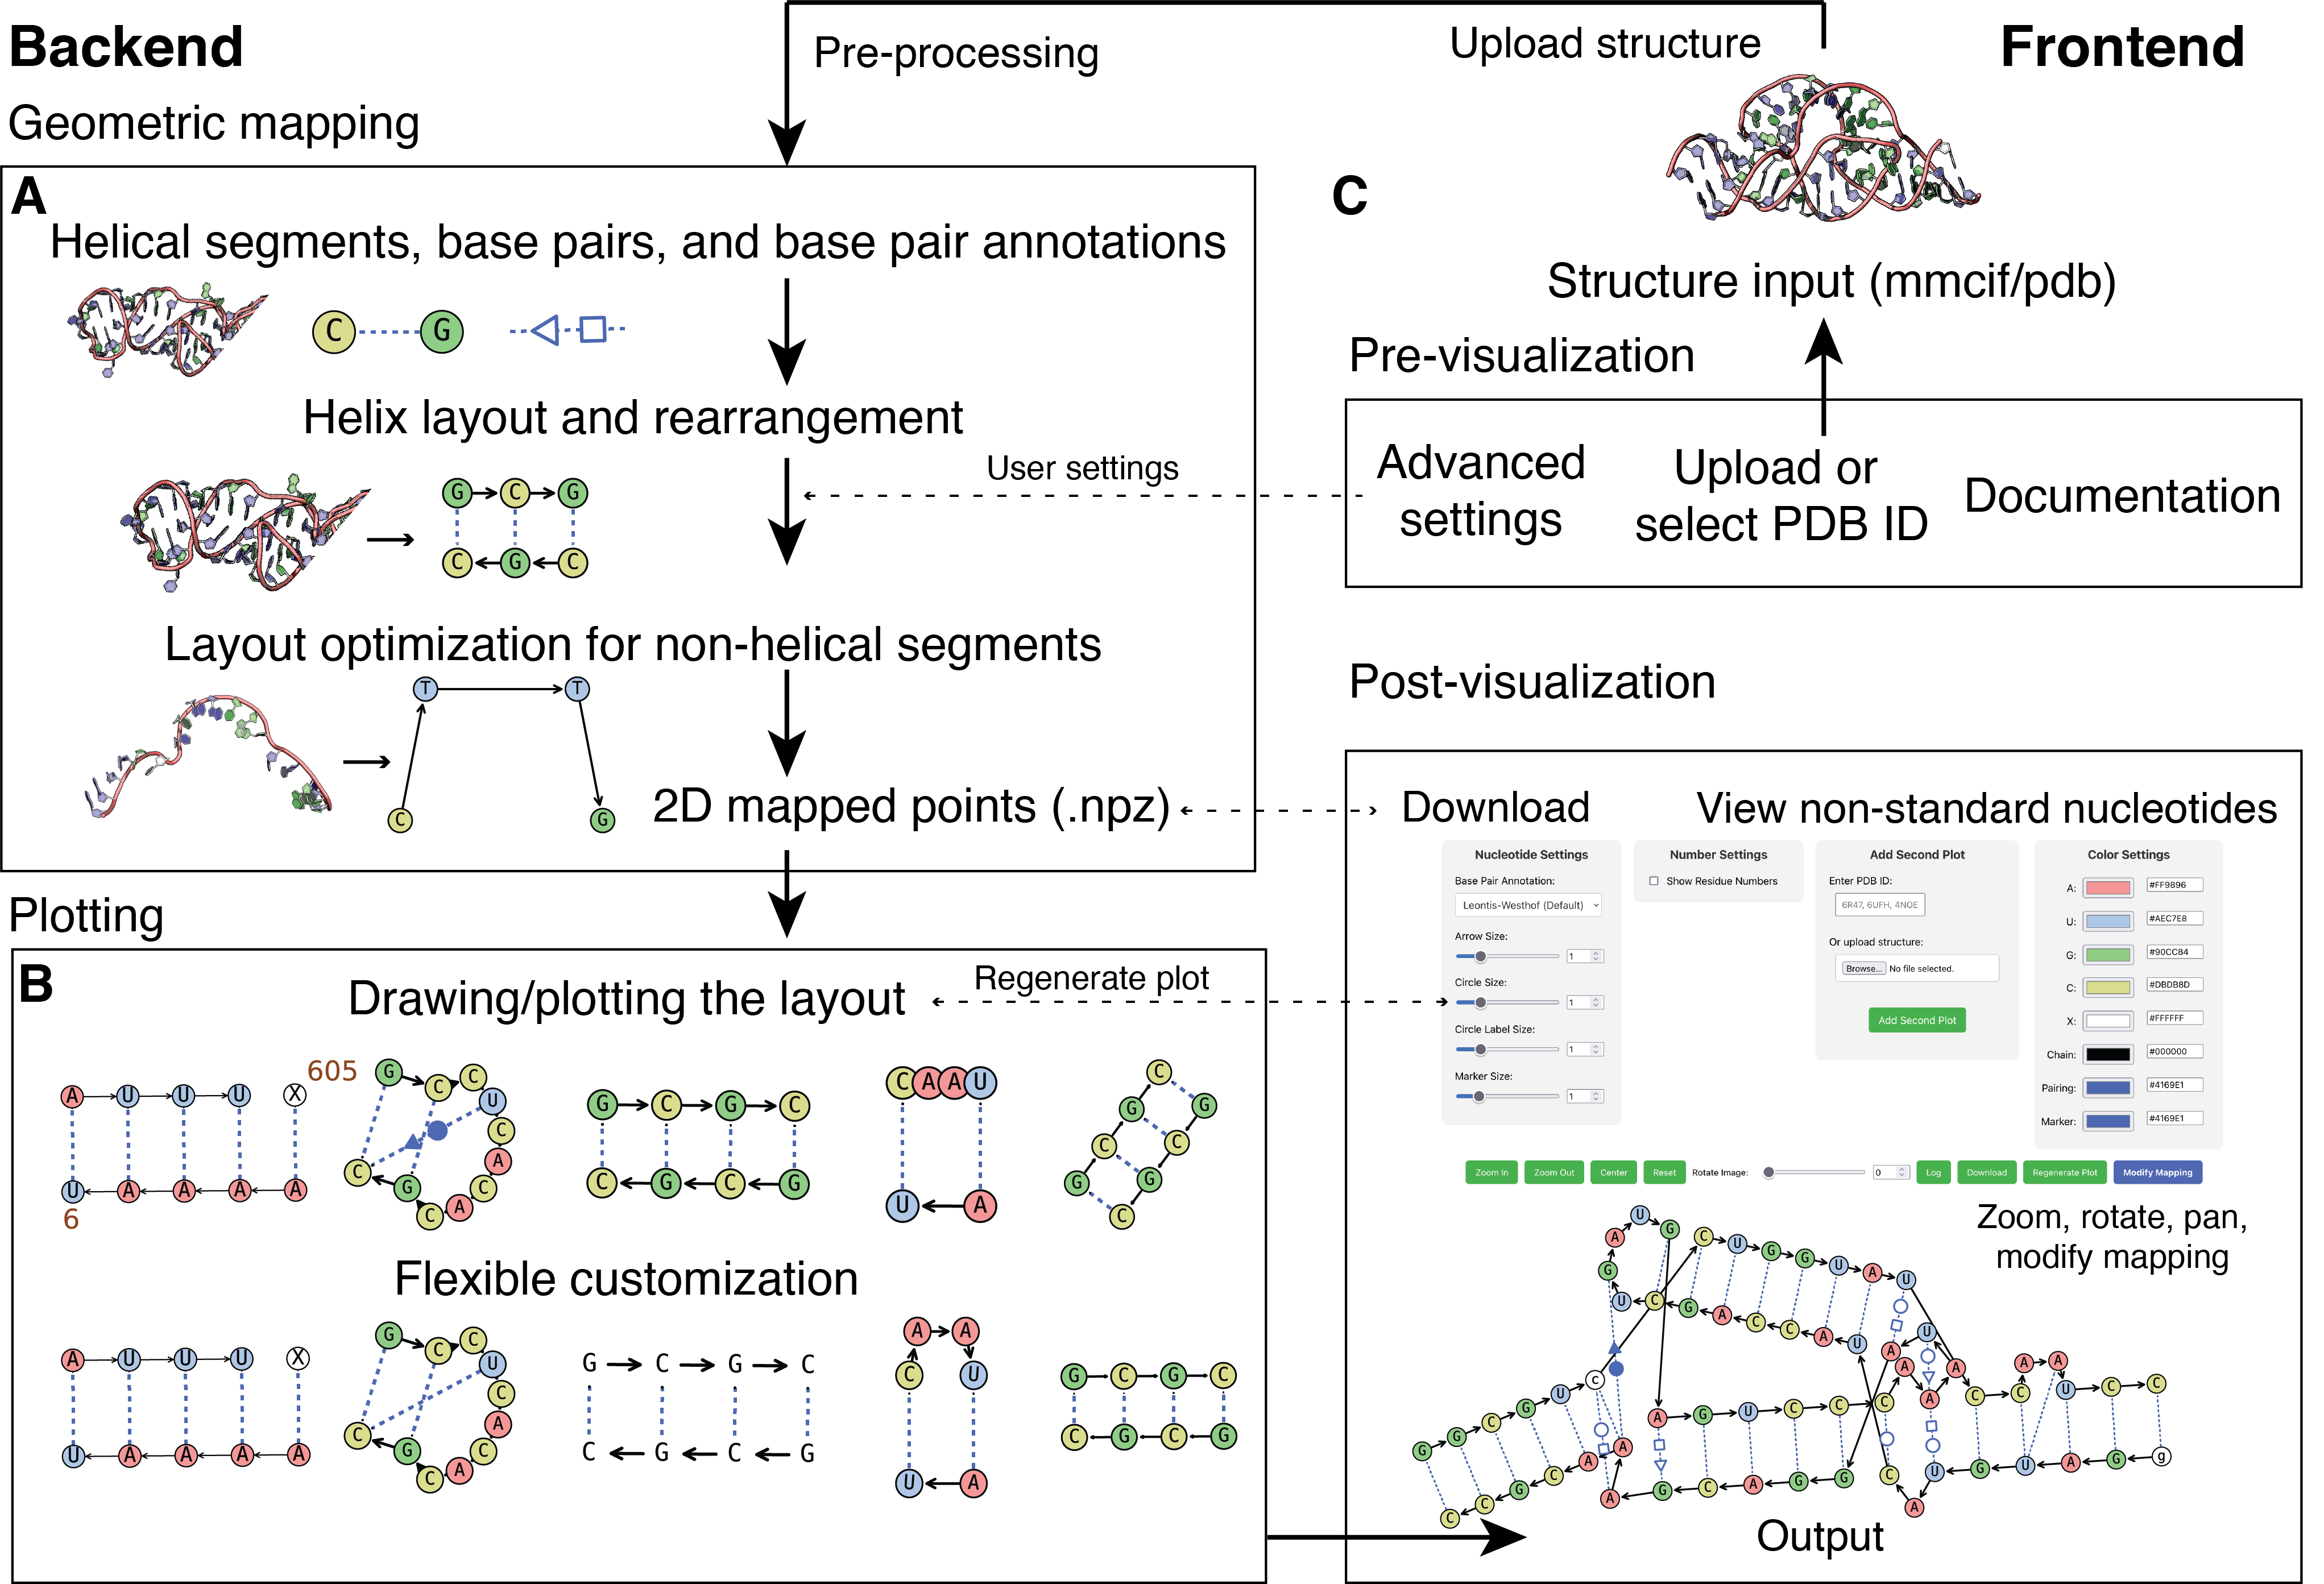
\includegraphics[width=0.8\paperwidth]{./rnascapefigs/figure2.png}}
 % archetecture.png: 1149x508 px, 72dpi, 40.53x17.92 cm, bb=0 0 1149 508
        \caption[Computational cost of training RVAgene]{\textbf{Training RVAgene is reasonably scalable on CPU and even more so using hardware acceleration through GPU.} ({\bf A}) Time cost of training RVAgene for 100 epochs for datasets with varying number of genes and time points on CPU and GPU. ({\bf B}) Maximum memory utilized during training of the model on CPU an GPU for the cases in (A), inset plot: comparison of max memory used compared to DPGP for varying number of genes.}
  \label{fig:rnascape2}
\end{figure}
\end{center}


%\section{Results}
\subsection{Application of RNAscape to structures from the PDB}

We present RNAscape output for various structures (\hyperref[fig:rnascape4]{Fig. 3.1}, \hyperref[fig:rnascape4]{3.4} from the PDB \citep{berman2000protein}). In \hyperref[fig:rnascape1]{Fig. 3.1A}, tRNA from Sulfolobus tokodaii (PDB ID: 7VNV) is shown. RNAscape output preserves the L-shaped topology (as opposed to known ‘clover leaf’ shaped secondary structure \citep{Krahn2020} visualizations) and annotates non-standard bases and base-pairing geometries (critical in many RNA interactions \citep{Hermann1999}. RNAscape can also process unusual DNA structures, as shown by a single-stranded DNA with circular topology (PDB ID: 4NOE, \hyperref[fig:rnascape1]{Fig. 3.1B}). In \hyperref[fig:rnascape1]{Fig. 3.1C}, Dengue virus RNA promoter (PDB ID: 7UMD) is depicted, which is a single-stranded RNA molecule containing only standard RNA bases.

We present a few different examples of ribozymes and riboswitches (\hyperref[fig:rnascape1]{Fig. 3.1D-G}). RNA loop modeling \citep{Sripakdeevong2011} for riboswitches is an important area of research, and RNAscape visualizations (e.g. PDB IDs: 1Y26, 4FRN, 8HBA, \hyperref[fig:rnascape1]{Fig. 3.1E-G}) may aid in these efforts. The pistol ribozyme (PDB ID: 6R47, \hyperref[fig:rnascape1]{Fig. 3.1D}) and the Nicotinamide Adenine Dinucleotide-II (NAD-II) riboswitch (PDB ID: 8HBA, \hyperref[fig:rnascape1]{Fig. 3.1G}) illustrate how RNAscape places non-helical segments and can clearly depict their non-standard base pairs with helical segments. RNAscape natively supports multiple strands (e.g. PDB ID: 1Y26, \hyperref[fig:rnascape1]{Fig. 3.1E}). RNAscape is also able to visualize G-quadruplexes (PDB ID: 2M18, \hyperref[fig:rnascape1]{Fig. 3.1H}). An RNA structural motif which can serve as a binding site for proteins is the kink-turn motif (PDB ID: 7EFG) \citep{Schroeder2010}, and it is visualized in \hyperref[fig:rnascape1]{Fig. 3.1I}.

There has been a continued interest in structural studies of the ribosome which postulate the role of a proto-ribosome \citep{Bose2022} in the origin of life. The proto-ribosome is a semi-symmetrical core of the ribosome comprised of RNA molecules representing the site for peptide bond formation, therefore known as peptidyl transferase center (PTC). The RNAscape visualization (\hyperref[fig:rnascape1]{Fig. 3.1J}, Supplementary \hyperref[fig:rnascapeS1]{Fig. S13}) for the same reflects the high degree of conformational symmetry, based on structural coordinates of the PTC provided by Bose et al. \citep{Bose2022,}.

RNAscape can run on relatively large structures (structures of up to 50 MB are processed by the webserver). In \hyperref[fig:rnascape4]{Fig. 3.4}, we demonstrate its application to four different topologies of larger structures. In \hyperref[fig:rnascape4]{Fig. 3.4A}, a triangular topology of Mycobacterium tuberculosis ileS T-box in complex with tRNA (PDB ID: 6UFH, 244 nucleotides) is shown, followed by a diamond-like topology of mutant P4-P6 domain of Tetrahymena thermophila group I intron (PDB ID: 1HR2, \hyperref[fig:rnascape4]{Fig. 3.4B}, 157 nucleotides) and an exon free state of the Tetrahymena group I intron (PDB ID: 7R6N, \hyperref[fig:rnascape4]{Fig. 3.4C}, 354 nucleotides). Secondary structure representations will not resemble the structure at all for many of these cases (e.g. stacked ladders, PDB ID: 7QDU, \hyperref[fig:rnascape4]{Fig. 3.4D}, 552 nucleotides), while RNAscape is able to reflect the 3D topology of these large RNA molecules.
\begin{center}
    \begin{figure}
    \makebox[\textwidth]{\includegraphics[width=0.8\paperwidth]{./rnascapefigs/figure3.png}}
 % archetecture.png: 1149x508 px, 72dpi, 40.53x17.92 cm, bb=0 0 1149 508
        \caption[RNAscape algorithm.]{\textbf{RNAscape algorithm.} ({\bf A})  Pre-processing of uploaded/fetched structures. Structure files are obtained either through user upload or direct download from the PDB. DSSR is run on each structure to detect helical segments and assign base-pairing annotations. ({\bf B}) Geometric mapping and post-processing of helical segments. For each helical segment, RNAscape estimates the ladder axis by connecting the centroids of the starting and ending nucleotides with a line segment. If a helix is bent, detected by a distance >10 Å between the midpoint of the ladder axis and corresponding helical segment's centroid, the ladder axis is split into two. Helical projections within 20 \AA and 30$^{\circ}$ are optionally merged. Base pairs are uniformly spaced along each ladder axis, and cramped helices are lengthened. ({\bf C}) Optimizing placement of non-helical regions followed by creation of annotated visualization. Hanging single stranded regions are mapped to their corresponding, connected helix and merged with the ladder. Loops are either preferentially bulged out in a radial curve or interpolated linearly based on a spatial density threshold. Loop direction is determined by minimizing the total nearest neighbor count of a given loop. Mapped points as well as pairing and backbone annotations are passed to the plotting script to create a visualization.}
  \label{fig:rnascape3}
\end{figure}
\end{center}
\subsection{RNAscape user interface}

The RNAscape webserver (\hyperref[fig:rnascape2]{Fig. 3.2C}) displays three primary items: header, file upload, and documentation panels. In the header, a user can click the ‘Run on Example Data’ button to view an example visualization (PDB ID: 3ZP8). In the file upload panel, a user can upload a structure using the file upload feature. This file may contain non-nucleic acid entities which will be ignored. Alternatively, a user can directly input a PDB ID to load its corresponding first assembly file. Clicking the ‘Run’ button runs the RNAscape pipeline on the uploaded structure file or provided PDB ID (biological assembly 1). After running RNAscape for a structure, a user has the option to add a second structure for side-by-side viewing. We demonstrate this capability for two structures of tRNA molecules (PDB IDs: 8UPT and 8UPY, Supplementary \hyperref[fig:rnascapeS2]{Fig. S14}), introduced by recent work \citep{Krahn2024} on the importance of tRNA shape. The documentation panel enables easy navigation and provides a quick start guide, tips, and examples for using RNAscape. It also includes detailed explanations for configurable settings.

\subsection{Output images}

The frontend (\hyperref[fig:rnascape2]{Fig. 3.2C}) natively supports touch-screen compatible image exploration. A user can zoom, center, or reset any zooming/panning via buttons above the display box. The image can also be rotated using a slider, and a ‘regenerate’ button is offered that replots the image, associated annotations, and user customizations in the desired rotation. To the right of the image, a legend is displayed that corresponds to the base-pairing annotation selected by the user. For the Saenger \citep{Saenger1984} base-pairing annotation, no legend is shown. The local strand direction ($5'$ to $3'$) is indicated by the black arrows between nucleotides for all plots. Other interactions are shown in blue dotted lines. These colors are fully customizable by the user. The user also has the option of downloading RNAscape mapped points in a numerical format (.npz) processable by the NumPy \citep{harris2020array} library. Additionally, a log is provided which contains a description of the non-standard/modified nucleotides in the plot and other associated information.

\subsection{Base-pairing annotations}

RNAscape offers three base-pairing annotation styles: LW \citep{Yang2003, Leontis2001}, DSSR \citep{lu2015dssr} and Saenger \citep{Saenger1984}. All base-pairing annotations are calculated via DSSR, although any future updates to these conventions by the nucleic acid community can be easily incorporated. Annotations do not affect geometric mapping, and a user can forego an annotation altogether. The LW annotation contains two key parameters: bond orientation (cis/trans) and base edge type. Bond orientation is represented by a filled or unfilled marker. The edge types: Watson-Crick (W), Hoogsteen (H), or sugar (S), are represented by marker shapes (\hyperref[fig:rnascape1]{Fig. 3.1}).

The DSSR style differs in that base edges are delineated by major groove (M), minor groove (m), or Watson-Crick (W) edges. Bond orientation annotation is the same as in the LW \citep{Yang2003, Leontis2001} annotation. DSSR also reports local strand orientation as a base-pairing annotation feature. RNAscape always denotes local strand orientation by the backbone arrows (\hyperref[fig:rnascape1]{Fig. 3.1}). Non-standard pairings flagged as ‘not categorized’ by DSSR are not annotated. For the Saenger \citep{Saenger1984} annotation, each bond type is represented by a number corresponding to its Roman numeral annotation.

\subsection{Customizable settings}

Several custom settings options are available (\hyperref[fig:rnascape2]{Fig. 3.2C}). The Loop Bulging setting controls whether loops are bulged outwards or linearly interpolated (see Materials and Methods). Additionally, the post-processing step of merging proximate, similarly oriented ladders can be turned off (\hyperref[fig:rnascape3]{Fig. 3.3B}). Since these settings affect the geometric mapping, a user must click ‘Run’ to run the pipeline again if they are changed. Arrow size, circle size, and circle label size affect nucleotide appearance. Base-pairing marker sizes can also be adjusted. Through the number settings, a user instructs RNAscape to label residue numbers in the numbering schema defined by the structure file. Color, size, frequency, and spacing of these labels can also be modified. Color settings allow a user to customize the color of each nucleotide type: A, C, G, U/T and X (non-standard nucleotides). Colors used to denote both backbone chain and non-chain interactions and markers can also be modified. Furthermore, RNAscape provides a functionality to modify calculated maps. By clicking on the ‘Modify Mapping’ button, the user can move and adjust nucleotide locations to resolve, for instance, overlap and regenerate the output.
\begin{center}
    \begin{figure}
    \makebox[\textwidth]{\includegraphics[width=0.7\paperwidth]{./rnascapefigs/figure4.png}}
 % archetecture.png: 1149x508 px, 72dpi, 40.53x17.92 cm, bb=0 0 1149 508
        \caption[RNAscape output for large-size structures from the PDB.]{\textbf{RNAscape output for large-size structures from the PDB.} The 3D structure at the top of each panel is from the PDB structure, with its corresponding RNAscape visualization shown below it. ({\bf A}) \textit{Mycobacterium tuberculosis} T-box in complex with tRNA (PDB ID: 6UFH, 244 nucleotides), ({\bf B}) Mutant P4-P6 domain (DELC209) of \textit{Tetrahymena thermophila} group I intron (PDB ID: 1HR2, 157 nucleotides), ({\bf C}) Exon-free state of the Tetrahymena group I intron (PDB ID: 7R6N, 354 nucleotides), and ({\bf D}) Twist-corrected RNA origami 5-helix Tile A (PDB ID: 7QDU, 552 nucleotides).}
  \label{fig:rnascape4}
\end{figure}
\end{center}

\section{Discussion}

The RNAscape webserver produces customizable, publication-quality visualizations of nucleic acid tertiary structure. It prioritizes the topology of a structure while striving to create a clean and optimized output, and it is designed to minimize user effort. RNAscape significantly deviates from any existing method in terms of its output quality, usability, and layout algorithm (\hyperref[table:rnascape]{Table 3.1}, Supplementary \hyperref[fig:rnascapeS3]{Fig. S13, S15}). Users can refine visualizations on the webserver, and RNAscape also supports non-standard nucleotides and various base-pairing annotations. Further updates to base-pairing conventions may be easily incorporated. The RNAscape webserver allows a maximum file size of 50 MB. While potentially informative, the output for extremely large structures may not be well suited for presentation. We provide the RNAscape implementation via GitHub (see Data Availability) for those inclined to try the pipeline locally on even larger structures. We conclude with the hope that our effort facilitates advancement of the ever-growing field of RNA biology

\section{Data availability}

RNAscape is freely available for all users at \url{https://rnascape.usc.edu/}. The backend implementation is also available on GitHub at \url{https://github.com/timkartar/RNAscape} and preserved through figshare at \url{https://doi.org/10.6084/m9.figshare.25201889}.
%%%%%%%%%%%%%%%%%%%%%%%%%%%%%%%%%%%%%%%%%%%%%%%%%%%%%%%%%%%%%%%%%%%%%%%%%%%%%%%%%%%%%%%%%%%%%%%%%%%%%%%%%%
\chapter{RNAproDB: a webserver and interactive database for analyzing protein–RNA interactions}
%\begin{abstract}

We present RNAproDB (\url{https://rohslab.usc.edu/rnaprodb/}), a new webserver, analysis piepline, database and highly interactive visualization tool designed for protein-RNA complexes and applicable on all forms of nucleic acid containing structures. The RNAproDB analysis of a structure involves computing several mapping schemes for nucleic acid components and presenting protein-RNA interactions appropriately. Various structural annotations are computed which include non-standard base-pairing interactions, hydrogen bonds, protein-RNA and RNA-RNA water mediated hydrogen bonds etc. This information is presented in the form of interconnected Sequence viewer, 3D viewer, Interface explorer, Secondary structure selector and tabular data. A novel feature, subgraph selection, is also implemented, which facilitate studying individual components of complex structures. We hope RNAproDB will be highly useful for analyzing and exploring not only experimentally determined, but also predicted or designed protein-nucleic acid complexes.

\end{abstract}
\section{Introduction}
Structural complexity of RNA molecules is vast and so are their modes of interaction with proteins \citep{jones2001protein}. Although there has been an ever-expanding repertoire of structural data on the PDB, there is a lack of data resources which systematically analyze these interactions. In addition, recent advances in artificial intelligence have made high throughput prediction of protein-RNA complex structures viable \citep{Abramson2024, watson2023novo}. RNAproDB is a webserver where a user can upload a protein-RNA complex and explore analyzed results covering a multitude of aspects (e.g., direct and water-mediated hydrogen bonds, base-pairing annotations, nucleotide modifications, secondary structural features). Compared to existing resources, which often focus on the RNA structure alone and provide a particular way of visualization \citep{Kerpedjiev2015, Yang2003}, or use a representation which is very coarse-grained \citep{chojnowski2014rna}, RNAproDB provides three different algorithms for visualizing the RNA topology along with the interacting protein residues: a new design based on partial projection of the structure (RNA and interacting protein residues), tertiary structure aware mapping \citep{Mitra2024rnascape}, secondary structure-based mapping \citep{Kerpedjiev2015}. This information is presented via a highly interactive interface explorer combined with sequence and 3D-structure viewers, and a secondary structure selector. Tabular data is also available. Another novel functionality, subgraph exploration, allows a user to explore parts of the structure (e.g., a particular junction region) via the interface explorer. Subgraph selections can be manually entered or automatically selected from the secondary structure selector. As of our knowledge, no existing tool offers such capability. In addition to the webserver, we offer pre-analyzed structures containing RNA, from the PDB, in the form of a searchable collection. With a cutoff of 10,000 monomers per biological assembly and molecular weight cut off of 800 kDa on the asymmetric unit, the initial collection of RNAproDB provides around 3,500 biological assemblies containing RNA molecules. RNAproDB will be automatically updated weekly with new PDB entries. We believe RNAproDB will be a valuable resource for the scientific community interested in RNA biology, protein-nucleic acid interaction and function, structure prediction, and drug design. This work is led by me, with contributions from Ari S. Cohen, Wei Yu Tang, Hirad Hosseini, Chan Hong, Prof. Helen Berman and supervised by Prof. Remo Rohs.

\begin{center}
    \begin{figure}
    \makebox[\textwidth]{\includegraphics[width=0.8\paperwidth]{./rnaprodbfigs/fig1.png}}
 % archetecture.png: 1149x508 px, 72dpi, 40.53x17.92 cm, bb=0 0 1149 508
        \caption[Multiple mapping algorithms available in RNAproDB for protein-RNA complex (PDB ID: 1IVS)]{\textbf{Multiple mapping algorithms available in RNAproDB for protein-RNA complex (PDB ID: 1IVS).} ({\bf A}) Crystal structure of the valyl-tRNA synthetase bound to tRNA (PDB ID: 1IVS).  ({\bf B})  Mapping produced based on partial projection. ({\bf C}) Mapping produced based on RNAscape algorithm. ({\bf D}) Mapping produced by applying ViennaRNA secondary structure layout algorithm. }
  \label{fig:rnaprodb1}
\end{figure}
\end{center}

\section{Processing pipeline}
The RNAproDB processing pipeline starts with a structure and computes multiple visualizations and interaction information from it. As part of the processing piepline multiple software are run, which include X3DNA-DSSR (\citep{Lu2015}computes base-pairing geometries, protein-RNA hydrogen bonds and RNA secondary structure), HBPLUS (\citep{McDonald1994} to compute hydrogen bonds involving water molecules), RNAscape (\citep{Mitra2024rnascape} tertiary structure aware nucleotide mapping), ViennaRNA (\citep{Lorenz2011} secondary structure-based nucleotide mapping), DSSP (\citep{joosten2010series, kabsch1983dictionary} computes protein secondary structure). In addition, custom code has been developed to compute a new ``Partial Projection" based mapping for the nucleotides. The processing pipeline combines all these data into a graph object which is used to compute highly interactive frontend presentation of the structure. This frontend presentation is an intertwined experience of an Interface explorer, a 3D viewer, a Secondary structure selector, a Sequence viewer and Tabular data. In the next sections we describe the functionalities implemented through these components.

\section{Interface explorer}

The 'Interface explorer' for RNAproDB is freshly designed to present an interaction graph of the RNA structure along with interacting protein residues. The explorer present three different layout algorithm options, selectable by the user. two of these options are secondary structure based (computed using ViennaRNA \citep{Lorenz2011}) and tertiary structure aware mapping based (computed using RNAscape \citep{Mitra2024rnascape}). The third (default) option is a new mapping scheme produced by prjecting the RNA residues and only interacting protein residues into the 2D plane maximizing their spatial variance \citep{Pearson1901}. We call this method ``Partial projection" (instead of the whole structure, it only projects the RNA and interacting protein components). In our observation, this scheme is visually intuitive for exploring corresponding 3D structure. The user is free to choose between the three layouts. In each case, the protein residues are placed using a force directed layout scheme \citep{bostock2012fl}. We demonstrate the three layout schemes for a valyl-tRNA synthetase-tRNA complex (PDB ID: 1IVS) (\blue{Fig. \ref{fig:rnaprodb1}A}). The partial projection-based layout is shown in \blue{Fig. \ref{fig:rnaprodb1}B}. This layout reflects the helical turns, making the best coreespondance with the 3D structure. The RNAscape \citep{Mitra2024rnascape} layout (\blue{Fig. \ref{fig:rnaprodb1}C}) is cleaner and more suitable for users used to a ladder-like representation.  The secondary structure based layout, shown in \blue{Fig. \ref{fig:rnaprodb1}D}, although familiar, suffers from tertiary interactions within RNA and protein-RNA interactions criss-crossing the view. Options to turn off tertiary interaction edges and protein interactions have been implemented to help with this situation, in case a user wants a clean view of the secondary structure. This is demonstrated in \blue{Fig. \ref{fig:rnaprodb2}A-C}). Another useful feature of the interface explorer is the ability to change distance theshold of visible protein-RNA interactions on the fly. This threshold can be modified using a slider, and upon modification, edge distances that fall beyond the threshold are hidden. The protein-RNA interactions shown were computed with an atom atom cut-off distance of 6 $\AA$, except for water-mediated hydrogen bond edges, which can have a longer distance. A protein residue interacting only with the major groove side or minor groove side (as in standard watson crick conformation) of a base are assigned special colors whereas alternate possibilities are left gray. In addition, protein-RNA interaction edges have a distance dependent opacity setting, making interactions which are further away, less prominent, thereby reducing visual clutter.
The distance threshold control provided with the interface explorer is operated on centroid-centroid distance between a protein residue and a nucleotide (0-15 $\AA$). At any point of the exploration, the user is able to download the visualization as a static picture, a scalable vector graphic format image or download the corresponding graphical data.

\section{Sequence viewer and 3D viewer}

In addition to the interface explorer, we also provide a 3D structure viewer and sequence viewer to facilitate the exploration process (\hyperref[fig:rnaprodbS2]{Fig. S30}). The sequence viewer lists sequences for each chain in the structure. A chain can be selected from a drop-down menu, resulting in the corresponding sequence being displayed. Selecting a residue/nucleotide from the sequence viewer highlights the corresponding residue/nucleotide in the Interface explorer. In addition, the 3D viewer will also zoom and orient to focus on the specific residue/nucleotide, which is now shown in a ball-stick view. If the subgraph selection dialogue box is open, this will also populate the dialogue box with the ID of the selected residue/nucleotide. Residues/nucleotides can also be selected from the 
Interface explorer (using single click, or multi-select using shift+click). Doing so will highlight them in the 3D viewer also, in a similar manner. Right clicking on consecutive atoms on the 3D viewer allows for visualizing measurements also. For the 3D viewer, buttons to show/hide carton representation and solvent is available.
\begin{center}
    \begin{figure}
    \makebox[\textwidth]{\includegraphics[width=0.8\paperwidth]{./rnaprodbfigs/fig2.png}}
 % archetecture.png: 1149x508 px, 72dpi, 40.53x17.92 cm, bb=0 0 1149 508
        \caption[Novel interactive capabilities of the RNAproDB user interface]{\textbf{Novel interactive capabilities of the RNAproDB user interface.} ({\bf A}) Secondary structure based layout of a protein-RNA complex (PDB ID: 1IVS) ({\bf B})  Updated layout with tertiary RNA interactions turned off. ({\bf C}) Updated layout with protein interactions turned off. ({\bf D}) 3D structure of a zinc finger protien-RNA complex (PDB ID: 1UN6). ({\bf E}) Corresponding secondary structure selector, a user can click on any node (example: stem3, circles) ({\bf F}) Partial projection based layout for PDB ID: 1UN6. ({\bf G}) Generated subgraph based on user selected secondary structure element.}
  \label{fig:rnaprodb2}
\end{figure}
\end{center}
\section{Secondary structure selector and subgraph exploration}

A more coarse grained diagram is also computed as part of the processing piepline for RNAproDB. This diagram reflects the different secondary structure elements as one node each, interaction edges corresponding to residues involved in one secondary structure element with another are collapsed into one edge. This view is presented to serve as a more coarse representation, components of which are selectable by the user, named "Secondary structure selector". An example is shown for PDB ID: 1UN6 \blue{Fig. \ref{fig:rnaprodb2}D}). The corresponding Secondary structure selector is shown in \blue{Fig. \ref{fig:rnaprodb2}E}. The partial projection-based layout for this structure is presented in \blue{Fig. \ref{fig:rnaprodb2}F}. 

Whenever a user clicks a particular node (e.g. `Stem 3' in \blue{Fig. \ref{fig:rnaprodb2}E}), corresponding nucleic acid residue ids are populated into the subgraph generation dialogue. The user can now click the "Generate subgraph" button to generate and explore the subgraph (upto first order neighbors) via the interface explorer (\blue{Fig. \ref{fig:rnaprodb2}G}). Beyond clicking the secondary structure selector, a subgraph selection can also be manually entered or selected from the Sequence viewer or Interface explorer. 

\section{Search functionalities and Upload}

The pre-analyzed collection of RNAproDB contains 3500+ protein-RNA structures. In addition, RNA structures without proteins, DNA and NA-hybrid containing structures are also included. A known PDB ID can be directly searched using the qucick search box available at the top-right location of the website. More refined searches can be performed from the "Search" page. The search page allows search queries to be entered which can be author names or keywords related to the structures of interest. Additional filters can be set, which include molecule type (polymer entity type: RNA/DNA/NA-hybrid), experimental modality, resolution range, publication year, number of NA polymers, number of protein polymers, molecular weight of the biological assembly. The search results will be presented in tabular view. Optionally a card view of the search results is also available. The resulting PDB IDs can be copied to clipboard or the data can be downloaded in comma-separated value (CSV) or JavaScript object notation (JSON) format. An example search output page for the keyword search ``tetrahymena" is shown in \hyperref[fig:rnaprodbS1]{Fig. S29}.

Structure files in mmCIF format can be uploaded to the RNAproDB webserver through the upload page. Upon upload, the server will process the structure and create a custom page with the results. We hope this feature will be exceedingly valuable for people looking to analyze predicted complex structures (e.g. from AlphaFold3 \citep{Abramson2024}) of protein and nucleic acids. An example output page for AlphaFold3 predicted structure (model 0) for molecules in PDB ID: 8AW3 is shown in \hyperref[fig:rnaprodbS2]{Fig. S30}. An example of Interface explorer layouts for a CAS9-DNA-RNA complex  is also presented in \hyperref[fig:rnaprodbS3]{Fig. S31}.

\section{RNA-RNA water mediated interactions}

Non-canonical base-pairing is very common in RNA structures and often they influence structural organisation of the molecule and interaction with other molecules \citep{olson2019effects}. Varied combinations of base pairings often lead to sub-optimal direct hydrogen bonds between pairs or adjacent bases. Water molecules appear to compensate such situations by making ``base-pairing" possible through water-mediated hydrogen bonds. One such example is the CUG repeat structure from PDB ID: 7Y2B (\citep{wang2023structural}, \blue{Fig. \ref{fig:rnaprodb3}A})). The U-U mismatches in this structure are often unable to form direct hydrogen bonds (specifically, the central U-U mismatch, forms no direct H-bond). Therefore, DSSR (\citep{Lu2015}) does not consider it a base-pair. However, two water molecules form water-mediated hydrogen bonds between the two U's. This has an effect on the structure, as the U-U mismatch region now has a similar base-pair width as the C-G paired regions (\blue{Fig. \ref{fig:rnaprodb2}D}), otherwise expected to be narrower in width). 

RNAproDB computes RNA-RNA water mediated hydrogen bonds to reflect such information in the interface explorer (\blue{Fig. \ref{fig:rnaprodb2}B}), which would otherwise be overlooked. We demonstrate the molecular conformation of the central U-U mismatch (\blue{Fig. \ref{fig:rnaprodb2}C}) and a off-center U-U mismatch (\blue{Fig. \ref{fig:rnaprodb2}D})

\begin{center}
    \begin{figure}
    \makebox[\textwidth]{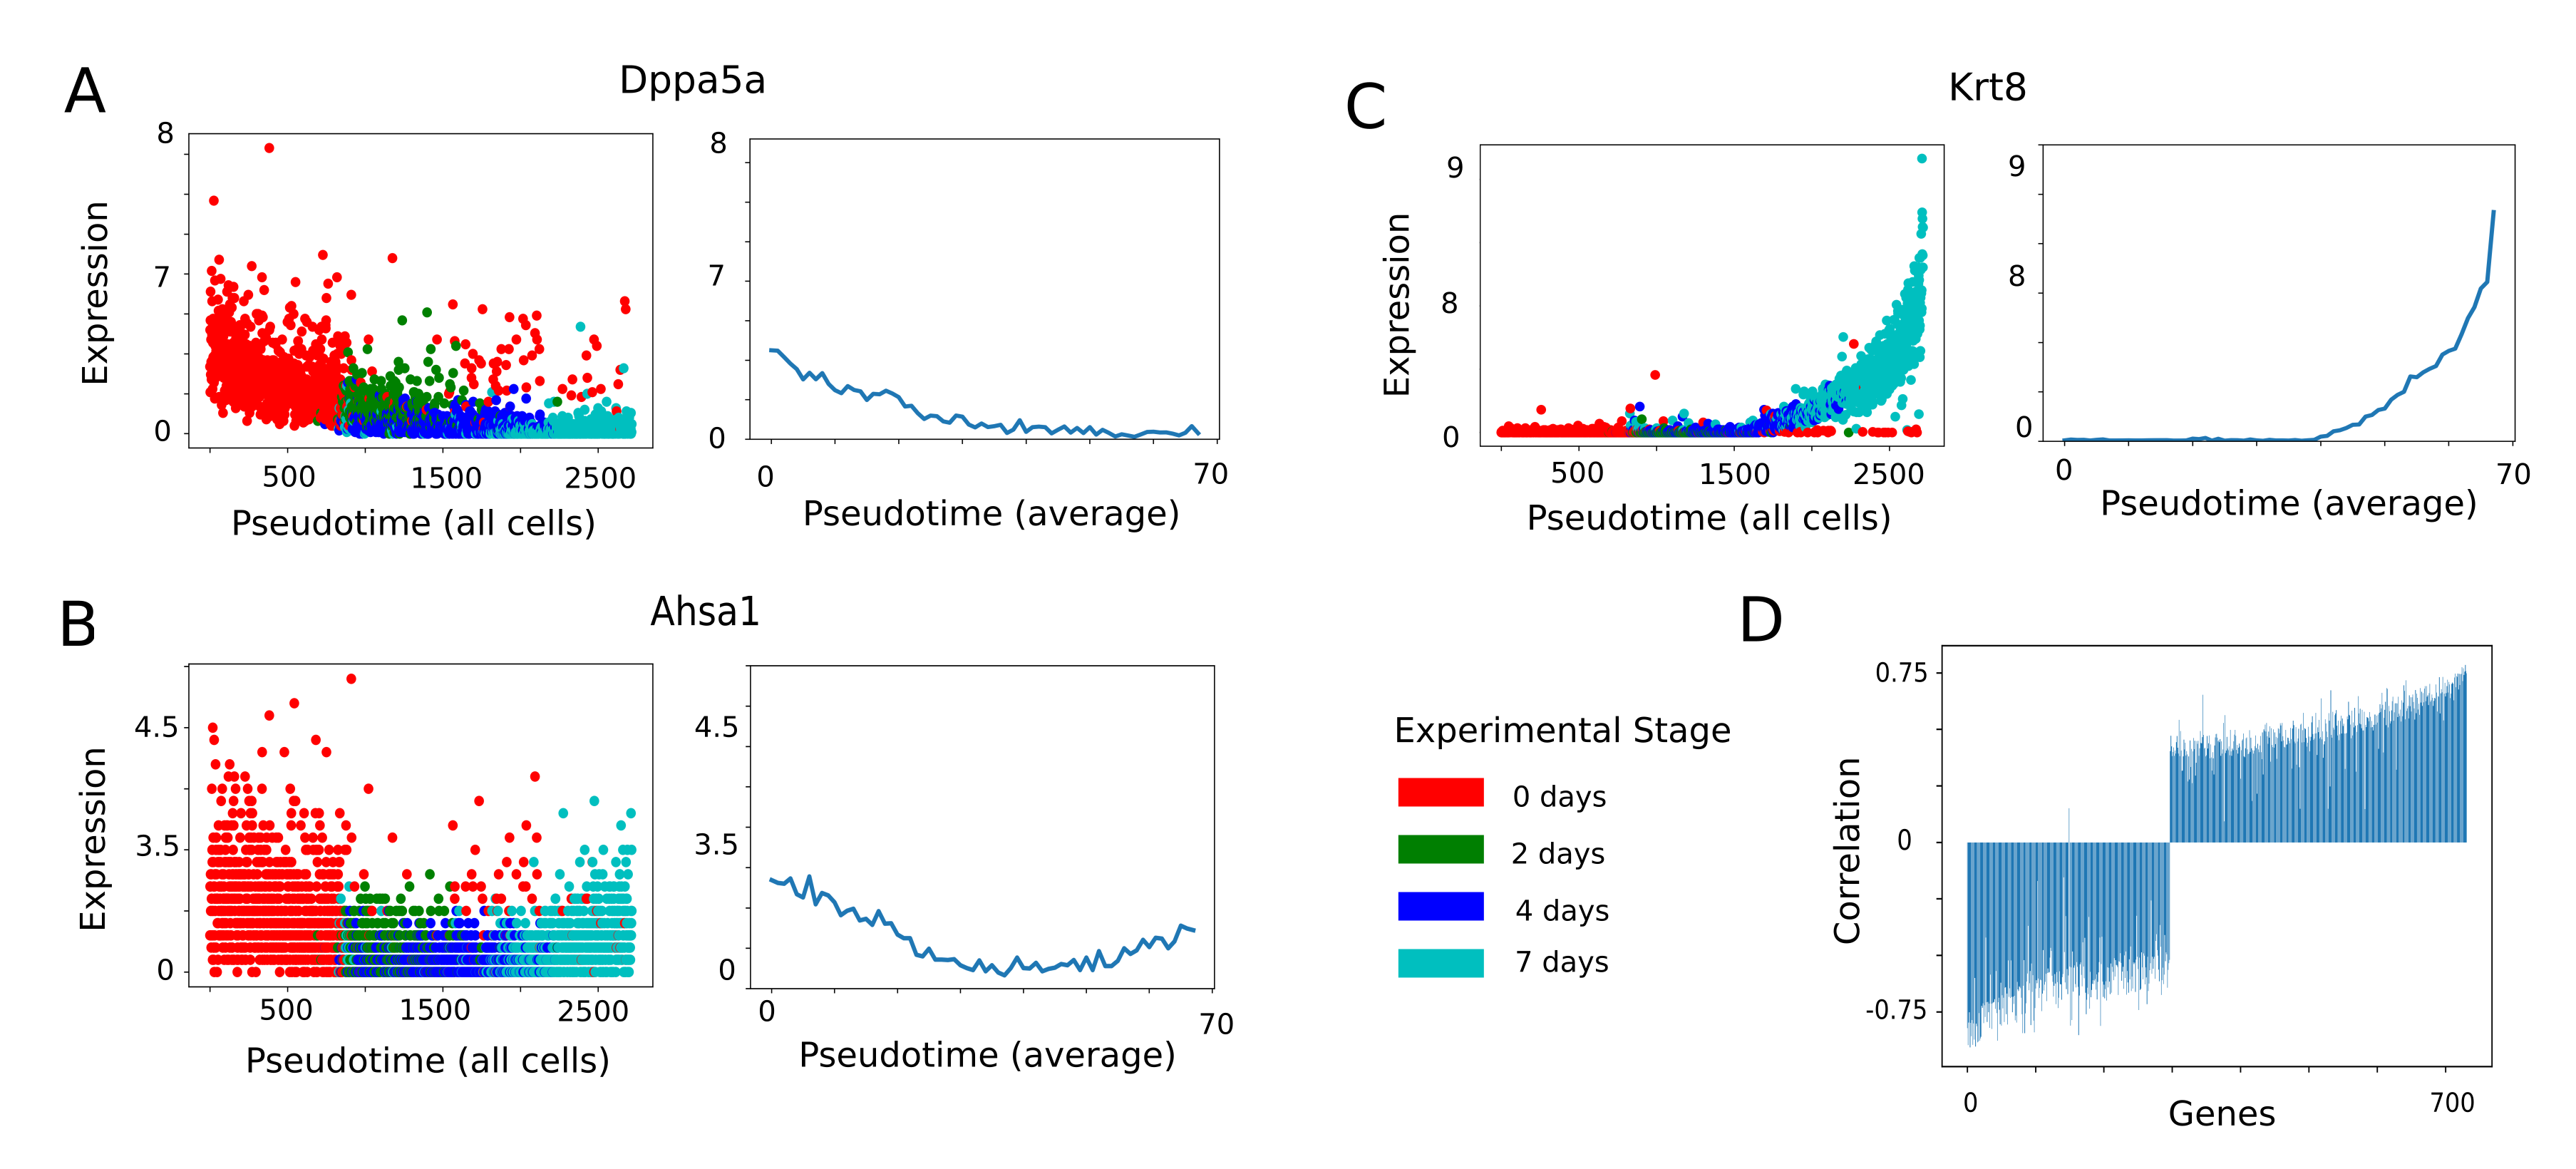
\includegraphics[width=0.8\paperwidth]{./rnaprodbfigs/fig3.png}}
 % archetecture.png: 1149x508 px, 72dpi, 40.53x17.92 cm, bb=0 0 1149 508
        \caption[Example illustration of RNA-RNA water mediated hydrogen bond facilitating non-Watson-Crick interaction.]{\textbf{Example illustration of RNA-RNA water mediated hydrogen bond facilitating non-Watson-Crick interaction.} ({\bf A}) 3D structure of PDB ID: 7Y2B  ({\bf B}) RNAproDB interface explorer layout (RNA scape algorithm) for PDB ID: 7Y2B. The central U-U is considered un-paired by DSSR, but computing RNA-RNA water-mediated hydrogen bonds reveal interactions between them. ({\bf C}) Zoomed in view of central U-U interaction with two water-molecules facilitating water-mediated hydrogen bonds. ({\bf D}) Zoomed in view of an off center U-U interaction with one water molecule facilitating water-mediated hydrogen bond in addition to a direct hydrogen bond.}
  \label{fig:rnaprodb3}
\end{figure}
\end{center}

\section{Discussion}

After working on RNAscape \citep{Mitra2024rnascape} and the DNAproDB \citep{Sagendorf2017, Sagendorf2020} update, we realized the lack of a modern software interface for structural analysis of protein-RNA interactions. DNAproDB, although an excellent tool, is geared, very specifically, towards DNA in many aspects. This precludes it from being applicable to nucleic acid structures in general. Here, we developed RNAproDB, targeting a broader class of protein-nucleic acid structures. This required innovating new ways of presenting the data and interface explorer (e.g. partial projection layout, subgraph exploration coupled with secondary structure selector etc.). RNAproDB provides access to NA-hybrid structures like Cas9 bound to target DNA and guide RNA \citep{nishimasu2014crystal,} and structures related to newly developed Bridge editing technique for genome editing \citep{durrant2024bridge}, which previously lacked an interface for analysis and interactive visualization. RNAproDB is also suitable for analyzing predicted complexes by recent advances like AlphaFold3 \citep{Abramson2024}. With the extensive list of novel capabilities described in this chapter, RNAproDB is the most modern tool for analyzing protein-nucleic acid structures which requires zero programming experience from the user. Further features like electrostatics of the protein-RNA interfaces are also currently in works. We hope RNAproDB serves as a valuable service and database for the structural and cellular biology community.

\section{Data availability}
RNAproDB is freely available for all users at \url{https://rohslab.usc.edu/rnaprodb/}.
The pipeline and frontend implementations are available via GitHub:
\url{https://github.com/timkartar/rnaprodb_dev}, and
\url{https://github.com/ariscohen/rnaprodb_frontend}.
%%%%%%%%%%%%%%%%%%%%%%%%%%%%%%%%%%%%%%%%%%%%%%%%%%%%%%%%%%%%%%%%%%%%%%%%%%%%%%%%%%%%%%%%%%%%%%%%%%%%%%%%%%

%%%%%%%%%%%%%%%%%%%%%%%%%%%%%%%%%%%%%%%%%%%% RVAgene ############################################################
% Research Topic 1
\chapter{Generative modeling of gene expression time series data}
\label{cha:research_topic_1}


\vspace*{0.35in}

\begin{flushleft}
% authors go here:
%{\large Raktim Mitra\textsuperscript{1},
%Adam L. MacLean\textsuperscript{1}}\\

%\bigskip
    Published at \href{https://dx.doi.org/10.1093/bioinformatics/btab260}{https://dx.doi.org/10.1093/bioinformatics/btab260}
%$^1$Quantitative and Computational Biology, University of Southern California
%\\

\end{flushleft}

%
\begin{abstract}
Methods to model dynamic changes in gene expression at a genome-wide level are not currently sufficient for large (temporally rich or single-cell) datasets. Variational autoencoders offer means to characterize large datasets and have been used effectively to characterize features of single-cell datasets. Here we extend these methods for use with gene expression time series data. We present RVAgene: a recurrent variational autoencoder to model gene expression dynamics. RVAgene learns to accurately and efficiently reconstruct temporal gene profiles. It also learns a low dimensional representation of the data via a recurrent encoder network that can be used for biological feature discovery, and from which we can generate new gene expression data by sampling the latent space. We test RVAgene on simulated and real biological datasets, including embryonic stem cell differentiation and kidney injury response dynamics. In all cases, RVAgene accurately reconstructed complex gene expression temporal profiles. Via cross validation, we show that a low-error latent space representation can be learnt using only a fraction of the data. Through clustering and gene ontology term enrichment analysis on the latent space, we demonstrate the potential of RVAgene for unsupervised discovery. In particular, RVAgene identifies new programs of shared gene regulation of {\em Lox} family genes in response to kidney injury.
\end{abstract}

%


\section{Introduction}
Dynamic changes in gene expression control the transcriptional state of a cell, and are responsible for modulating cellular states and fates. Gene expression dynamics are in turn controlled by cell-internal and external signaling networks. Despite the noisiness of gene expression in single cells \citep{raj2008nature}, over time or over populations of cells, predictable patterns emerge. Here we address the challenge of classifying and predicting gene expression dynamics across large groups of genes.
\par 
Machine learning (and deep learning in particular) has led to recent advances in our ability to explain or predict biological phenomena \citep{ching2018opportunities}. Deep learning modeling via autoencoders \citep{hinton2006reducing} and variational autoencoders \citep{Kingma2014} has been central to progress in the field. Autoencoders learn two functions: one to encode each input data point to a low dimensional point, and another (the decoder) to reconstruct the original data point from the low dimensional representation. Variational autoencoders (VAEs) build on this architecture and instead encode input data points as distributions; VAEs are less prone to overfitting and can offer meaningful representations of biological features in the latent space \citep{way2017extracting}.


%Another challenge is assessment i.e. how much better these methods are compared to some traditional methods for performing similar tasks because often the reported performances of these methods rely on heavy hyperparameter tuning [cite greene] and generalizing a model for different datasets might be hard with a given setting and hence doing a study of straightforward comparison of these methods is hard. The aspect of interpretability of deep networks also remain hard to address [cite stg interpretrable]. 
\par 
Single-cell mRNA sequencing (scRNA-seq) data present appealing sources of data for deep learning models, given their size and complexity \citep{svensson2018exponential}. Deep learning models have been used to analyze \scrna data and address a variety of challenges. Autoencoders have been developed to perform noise removal/batch correction \citep{deng2019scalable, eraslan2019single, wang2019data}, imputation \citep{talwar2018autoimpute}, and visualization \& clustering \citep{lin2017using}. VAEs have been developed for the visualization and clustering of \scrna data \citep{ding2018interpretable, wang2018vasc}, and can provide a broad framework for generative modeling of \scrna data \citep{lopez2018deep}: scVI can be used for batch correction, clustering, visualization, and differential expression testing.
%These methods offer exciting new avenues for discovery from single-cell profiling experiments, although limitations remain \citep{zheng2019emerging}.
\par 
The methods described above for single-cell data analysis by deep learning focus primarily on cell-centric tasks; here we are interested in gene-centric inference. Particularly, we are interested in characterizing dynamic changes in gene expression. These can be either changes with respect to real time or ``pseudotime,'' the latter referring to the ordering of single cells along an axis describing a dynamic cell process such as development or stem cell differentiation (see methods overview in \citep{saelens2019comparison}). We can interpret any \scrna data as gene expression time series data, given an appropriate underlying temporal process, either in terms of real (experimental) time (low resolution: around $2-20$ data points) or pseudotime (high resolution: $10^3-10^6$ data points). \citet{McDowell2018} introduced a non-parametric hierarchical Bayesian method (DPGP) to model such data. Using a Gaussian process to cluster temporal gene profiles and a Dirichlet process to generate the Gaussian processes, DPGP offers powerful and intuitive means with which to cluster gene expression time series data. However, since learning Gaussian processes is equivalent to a fully agnostic search in function space, training DPGP is computationally intensive and difficult to parallelize.  
\par
Clustering relies on strong assumptions about the underlying structure of the data. Even for methods that move away from hard clustering towards probabilistic methods for cell type assignment \citep{jetka2018information, zhu2019semisoft}, assumptions remain and under certain conditions a continuous representation of the data may be better. 
Here we take such an approach, and seek to find a low dimensional representation of the data, on which further analyses (including but not limited to clustering) can be performed. VAEs are an obvious choice, given their success on other \scrna analysis tasks, but modeling temporal changes with a feed-forward VAE would be equivalent to a fully agnostic search, similar to learning a Gaussian process. Recurrent networks offer well-established architectures for learning sequential and temporal data, and have been successfully combined with VAEs  \citep{Fabius2015}. We use a recurrent network architecture to take advantage of the structure in the data.
\par 
We introduce a recurrent variational autoencoder for modeling gene dynamics from \scrna data (RVAgene). RVAgene learns two functions during training, parameterized by encoder and decoder networks. The encoder network projects the training data into latent space (we use a 2 or 3 dimensions in order to visualize, though there are no inherent limits). The decoder network learns a reconstruction of training genes from their latent representation. RVAgene facilitates clustering of other characterization of gene profiles in the latent space. By sampling points from the latent space and decoding them, RVAgene provides means to generate new gene expression time series data, drawn from the biological process that was encoded. Overall, RVAgene serves as a multipurpose generative model for exploring gene expression time-series data. 
\par 
The remainder of the paper is structured as follows: we next present methodological details and development of RVAgene. We produce a synthetic gene expression time-series dataset with innate cluster structure, and demonstrate the accuracy of RVAgene on these data.
{We then explore two biological datasets with RVAgene: a \scrna dataset on stem cell differentiation over pseudotime, on which we demonstrate the advantages of RVAgene over alternative approaches; and a bulk RNA-seq dataset describing dynamic responses to kidney injury, on which we demonstrate the potential for biological discovery. We also present evidence for the efficiency and scalability of RVAgene, and we conclude by discussing its key features and limitations, in light of recent advances in machine learning that will pave the way for future work in these directions.
}

%\section{Methods}
We develop a recurrent variational autoencoder to model gene expression dynamics (RVAgene). Here we briefly describe the methods underpinning variational autoencoders, and present the implementation of RVAgene. 

\subsection{Variational inference and variational autoencoders}
In the most general setting of a Bayesian model, we seek to learn the latent variables $\vz$ that best characterize some data $\vx$. Given a generative process that draws latent variables from a prior distribution, $p(\vz)$, and a likelihood of the data observed that is given by $p(\vx|\vz)$, then the posterior probability is given by Bayes rule:
%Our target is to learn about $\vz$ given the observed $\vx$, which is governed simply by the Bayes' rule:
\begin{align*}
 p( \vz | \vx)&= \frac{p(\vx|\vz)p(\vz)}{\int_z p(\vx|\vz)p(\vz) dz}. \numberthis \label{bayes-rule}
\end{align*}
The denominator is often intractable, making it difficult to estimate $p( \vz | \vx)$. Markov Chain Monte Carlo methods provide means to estimate posterior probability distributions. 
An alternative method to estimate hard-to-compute probability distributions is Variational Inference (VI) \citep{Hoffman2013}, which starts from the assumption that the posterior can be approximated by a distribution $q(\vz)$ from the family $\cQ$. VI then amounts to an optimization problem to find the $q^*$ that minimizes the Kullback–Leibler (KL) divergence between the approximation and the true posterior: 
\begin{align*}
 q^*(\vz) &= \textrm{argmin}_{q(\vz)\in\cQ} \textrm{KL}(q(\vz)||p(\vz|\vx)). \numberthis \label{vi-formulation}
\end{align*}

Much recent effort has gone into solving VI problems in different settings \citep{Zhang2019, Ingraham2017, Bouchard-Cote2010}. VI can be framed as solving an optimization problem over function families: neural networks are popular candidates for representing and learning complex functions. VI was incorporated into autoencoders \citep{Kingma2014} to create the architecture of a variational autoencoder (VAE). A VAE consists of an encoder network to approximate $p(\vz|\vx)$ through a function $q_\vx(\vz)$, and a decoder network $p(\vx|\vz)$ (\hyperref[fig:fig2]{Fig. 1A}). Conceptually, the encoder solves an inference problem: approximating the posterior distribution $p(\vz|\vx)$ as some $q^*_\vx(\vz)$, while the decoder solves a reconstruction problem: defining a generative process for $p(\vx|\vz)$, given the latent variables.
The VAE posterior is modeled by a multivariate normal $\cN(\mathbf{\mu},\Sigma)$ of the same dimension as $\vz$. Training then comes down to minimizing two objective functions. For the encoder network, which should learn a ``well distributed'' latent space, minimize the KL divergence: KL$(\cN(\mathbf{\mu},\Sigma) || \cN(0,\vI)) $. For the decoder network, which should reconstruct the inputs $\vx$ from the latent space, minimizing either an $L1$ or $L2$ objective function with respect to $\hat{\vx}$ is appropriate. The use of KL-divergence and an $L2$ objective solves the VI formulation of Eq. \ref{vi-formulation} \citep{Kingma2014}, however, an $L1$ objective may be preferred in practice, e.g. in cases where we want to suppress the effects of outliers on the structure of $\vz$ \citep{botchkarev2018performance}.

% Each input point $\vx_i$ is encoded as a distribution over the latent space $\vz$ given a prior, \tcr{and also project $\vx_i$ to a point $\vz_i$ using the reparametrization trick (\cite{Kingma2014}).} Typically, VAEs typically use a standard normal prior $\cN(0,\vI)$ as the prior distribution over the latent space. The decoder network then takes points from the latent space $\vz$ as input, and generates $\vx$. 


%\begin{center}
%% 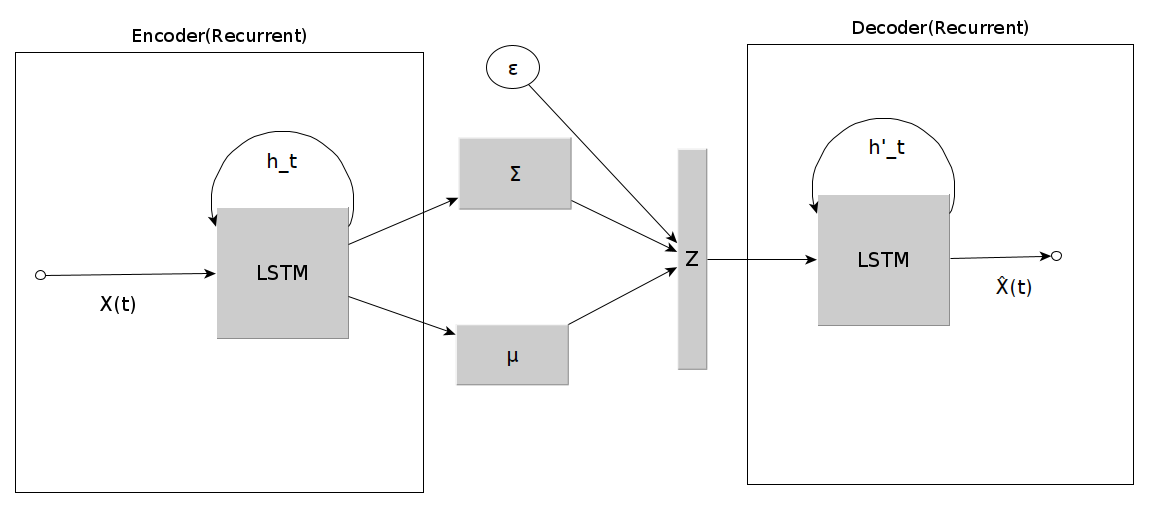
\includegraphics[scale=0.3]{architecture.png} 
%\begin{figure}
%\centering
%  \includegraphics[width=\linewidth]{figures/fig1.png}
% % archetecture.png: 1149x508 px, 72dpi, 40.53x17.92 cm, bb=0 0 1149 508
% \caption{Schematic diagram of RVAgene.}
% \label{fig:scheme}
%\end{figure}
%\end{center}


%% Probably too much detail here, but may want to cite the refs. 
%So far, we haven't specified anything about architecture of the encoder and decoder networks of a VAE, except that they learn certain functions modelling the posterior and likelihood probabilities  of our generative story of the data we are interested in. In general we could make them a fully connected neural network. But, since we are interested in handling sequential (time-series) data, we expect a specific structure of those functions. Intuitively, the $t$-th time point of input sequenece $\vx$ should be causally dependent only on its previous timepoints (upto $t-1$).  Therefore, instead of designing a completely agnostic network (e.g. fully connected layers), we can use a recurrent architecture for the encoder and decoder, which are well established in modelling sequence data (e.g. text data (\cite{Nallapati2016}), time-series data (\cite{Malhotra2015})). This in essence reduces the search space of the model from completely agnostic to a family of recurrent functions.
%\cite{Fabius2015} used this idea and showed how Recurrent Variational Autoencoders can be useful as a unsupervised latent representation learning and generative model for music data.


\subsection{RVAgene: A recurrent variational autoencoder to model gene expression dynamics}
Following the VAE architecture, RVAgene consists of an encoder and a decoder network with a reparameterization step in between. To incorporate the knowledge that we are modeling temporal data, recurrent neural networks offer an ideal architecture to use for both the encoder and the decoder networks. Recurrent and VAE networks have been successfully combined elsewhere, e.g. for textual \citep{Nallapati2016} and time series data \citep{Malhotra2015}.
\par
The architecture of RVAgene is based on \citet{Fabius2015}. An input sequence (i.e. gene) $x \in \vx$, $x = (x_1,x_2,...,x_t,...,x_T)$ is encoded using a recurrent function described by a long short-term memory (LSTM) unit. LSTM units are the state-of-the-art in recurrent architectures, since they are robust against the vanishing gradient problem for longer sequences, unlike other recurrent units (see details in \citet{Hochreiter1997}). We encode $x$ in the following manner:
\begin{align*}
 h_{t+1}^{enc} &= \textrm{LSTM}(W_{enc}^Th_t^{enc} + W_{inp}^T{x_t}+b_{enc}), \numberthis \label{lstm}
\end{align*}
where ($W_{enc}$, $W_{inp}$ and $b_{enc}$) are network weight parameters, and the hidden states $h_t$ represent information shared over timepoints in the LSTM. The dimension of the $h_t$ (and  $W_{enc}$) is given by a hyperparameter (``hidden-size''). The encoded $h_{t+1}$ are used to parametrize the posterior mean and variance from $x$, with mean $\mu_z$ and diagonal covariance $\sigma_z$ as:
%represent this mean and diagonal covariance matrix of the normal distribution an input $x$ is getting encoded to. 

\begin{align*}
 \mu_z &= W_{\mu}^Th_{T+1}^{enc} + b_{\mu} \numberthis \label{mu}\\
  log(\sigma_z) &= W_{\sigma}^Th_{T+1}^{enc} + b_{\sigma}.  \label{sigma}
 \end{align*}
We then use the reparameterization step described in \citet{Kingma2014} to sample $z$ from the distribution:
\begin{align*}
 z = \mu_z + \epsilon\sigma_z, \numberthis 
\end{align*}
where, for known $\epsilon$, backpropagation through the sampling step is possible while training the network.
\par
For the decoder network, the first state $h_1$ is calculated from $z$, and the recurrent formulation follows by reconstructing $x$ as $\hat{x} = (\hat{x}_1,\hat{x}_2,...,\hat{x}_t,...,\hat{x}_T )$, thus:
\begin{align*}
 h_1^{dec} &= \textrm{sigm}(W_{z}^Tz + b_{z})   \\
h_{t+1}^{dec} &= \textrm{LSTM}(W_{dec}^Th_t^{dec} + W_{out}^T{\hat{x}_t}+b_{dec}) \numberthis \label{decoder_lstm} \\
\hat{x}_t &= \textrm{sigm}(W_{out}^Th_t^{dec} + b_{out}), \\
\end{align*}
where $\textrm{sigm}(u) = \frac{1}{1 + e^{-u}}$ is the sigmoid activation function, and ($W_i, b_i$) are the network weight parameters. A schematic diagram of the network is shown in \hyperref[fig:fig2]{Fig. 1A}, which can now be trained using backpropagation, to minimize the objective function: 
\begin{align*}
    \cL(\theta, x) = D_{KL}(\cN(\mathbf{\mu}_z,\Sigma_z)||\cN(\mathbf{0},\vI)) + |x - \hat{x}|, \numberthis \label{lossfunction}
\end{align*}
where $\mathbf{\mu}_z$ and $\Sigma_z = \textrm{diag}(\sigma_z)$ are calculated from $x$ by the encoder.
\par 
To evaluate the accuracy of RVAgene, we need an appropriate error measure. For each gene in the test set, we calculate the $L1$ reconstruction error between generated data $\hat{x}$ and true data $x$, averaged over all time points. We normalize the data to lie in $[0,1]$ to avoid skewing the error by differences in gene expression magnitudes. Thus we define:
\begin{align}
    \textrm{Reconstruction error}(x,\hat{x}) = \frac{1}{T}\sum_{t}| s(\hat{x})_t - s(x)_t |,  & \text{ where } s(x) = \frac{x}{\sum_{t=1}^Tx_t}.
\end{align} 

\subsection{Generating synthetic gene expression time series data}
To test RVAgene, we generate a synthetic time series dataset. Six clusters each containing 20 genes are simulated, where for each cluster $c$, the mean gene expression time series $Y_c = (y_{c1}, y_{c2}, ..., y_{ct})$ was generated using addition or convolution and rescaling of two random sinusoidal functions of the form $k_1\textrm{sin}(k_2t)$, where $k_1,k_2$ are randomly chosen positive integers. Trajectories of cluster members were then generated by sampling from the multivariate normal $\cN(Y_c,\Sigma_c)$. We model $\Sigma_c$ as the positive definite matrix $\alpha Y_cY_c^T$, where $\alpha$ is a scaling factor, we use: $\alpha = 1/|Y_c Y_c^T|$. As defined, $\Sigma_c$ will describe nonzero correlations for all pairs of time points, $(t_i,t_j)$. This is unrealistic, so we set to 0 the entries of $\Sigma_c$ for which column and row indices have a difference of more than some threshold $T$ (we used $T=50$), reflecting the fact that correlations between time points are lost over larger time windows (temporal correlations are local). Note that under this condition, $\Sigma_c$  is no longer necessarily positive definite. The multivariate Gaussian sampler \verb+numpy.random.multivariate_normal()+ implemented in \verb+numpy+ \citep{harris2020array} was used to sample from this augmented $\Sigma_c$.
{After generating a simulated dataset by this process, we also added Gaussian noise, drawn from $\cN(0,0.7)$, to the simulated dataset to produce an additional dataset exhibiting higher levels of noise.}



\section{Results}
%
\subsection{RVAgene can accurately and efficiently reconstruct temporal profiles from synthetic data}
We generated a dataset of 120 genes using convolutions of sinusoidal functions (see Methods) to test
the ability of RVAgene (\hyperref[fig:fig2]{fig. 6.1A}) to learn and reconstruct noisy nonlinear
temporal profiles. An RVAgene model was trained on all 120 genes from 6 clusters with a hidden size
of 70 and a 3 dimensional latent space. The model was trained for 400 epochs, after which the
average batch objective $\cL$ function indicates convergence (\hyperref[fig:fig2]{fig. 6.1B}),
producing a three-dimensional latent space representation (\hyperref[fig:fig2]{fig. 6.1C}). K-means
clustering on the latent space (k=6) identified well-separated clusters (\hyperref[fig:fig2]{fig. 6.1D}).
%Thus, RVAgene has learnt a latent space in which different temporal profiles can be readily identified and classified using simple clustering methods. 


{\centering
\begin{figure}
  \includegraphics[width=\linewidth]{figures/fig2.png}
 % archetecture.png: 1149x508 px, 72dpi, 40.53x17.92 cm, bb=0 0 1149 508
    \caption[Unsupervised representation learning with RVAgene using synthetic data.]{\textbf{Unsupervised representation learning with RVAgene using synthetic data.} ({\bf A}) Schematic diagram of the RVAgene model. ({\bf B}) Average loss function $\cL$ as over duration of training.
    ({\bf C}) Latent space representation learnt by RVAgene model after training.
    ({\bf D}) Clusters detected by $k$-means clustering on the latent space, with $k=6$
    ({\bf E}) First and third rows show input training data used (20 simulated genes in each of six clusters); cluster means shown in black. Second and fourth rows show the model-generated data, obtained by sampling and decoding points from the latent space; decoded cluster empirical means shown in black.} 
 \label{fig:fig2}
\end{figure}
}
%%\tcr{I'm not sure about this in light of Svensson et al. we should discuss it.} 
RVAgene modeling followed by k-means clustering on the latent space identified 6 clusters with perfect fidelity between predicted and true clusters. One might reasonably ask, why use a neural network for this task? Simpler dimensionality reduction methods (e.g. PCA, t-SNE, or a non-variational autoencoder) would also find the correct solution. RVAgene has the advantage over these methods that the underlying structure of the latent space leads to interpretability. A point in reduced PCA or t-SNE space that does not overlap with a data point is not interpretable. Traditional autoencoders lack regularity in the latent space, i.e. even for a representation with arbitrary accuracy (a reconstruction error of zero), decoding a point that does not correspond to a training data point can result in nonsensical generated data, even if the decoded point is arbitrarily close to a training data point. Variational Auoencoders remedy this by learning a regularized or smoother distribution on the latent space. In this sense, the KL-divergence term in the VAE loss function can be thought of as a regularizer. This property enables RVAgene to generate new gene expression dynamics by decoding points from different regions of the latent space, having properties similar to clusters nearby to those points.


To demonstrate the generative properties of the RVAgene latent space, we sample points from
multivariate Normal distributions, centered on the empirical mean of each cluster with variance of
0.4, i.e. $\cN(\mu_c, 0.4I)$, where $\mu_c$ is the empirical mean of the cluster and $\vI$ is the
identity matrix in $\mathbb{R}^3$. Corresponding to each cluster, we sample 20 points in the latent
space, and use the decoder network to generate new time series data (\hyperref[fig:fig2]{fig. 6.1E}). Most of the points sampled generate trajectories that belong to the correct cluster. Moreover, we identify cases  corresponding to transitions between clusters. For example, some points sampled near Cluster 2 generate trajectories that are similar to members of Cluster 4, and vice versa. This makes sense due to the similarity between the temporal profiles of Clusters 2 and 4. A similar correspondence is observed between Clusters 1 and 5.
{We note that in a few cases the generated data have profiles that differ from their cluster of
origin and appear most similar to those of another cluster. This occurs when points are sampled
close to neighboring clusters, e.g. the red line for Cluster 5 in \hyperref[fig:fig2]{fig. 6.1E} has been sampled from a point close to cluster 3.}
We also observe some generated trajectories that display intermediate profiles between two or more clusters: the decoder function learnt by RVAgene is smooth, and gives rise to meaningful representations of points across regions of the latent space. 
\par
RVAgene offers additional functionality as a tool for removing noise from the data. Via sampling and
decoding points from the latent space, RVAgene reconstructs trajectories that are smooth and
de-noised relative to the input data (\hyperref[fig:fig2]{fig. 6.1E}, \hyperref[fig:figS1]{Fig. S16}). Similar neural network approaches have been proposed to denoise from single-cell data, e.g. using a deep count autoencoder \citep{eraslan2019single}. RVAgene provides data denoising as a by-product of its primary functionality: learning patterns of dynamic gene expression.
\par
{To investigate the impact of input noise levels on RVAgene performance, we added Gaussian noise
drawn from $\cN(0,0.7)$ to the simulated data to produce a dataset with higher overall noise levels.
RVAgene learns a latent space shown in (\hyperref[fig:figS1]{Fig. S16A}) from which six clusters are
identified by k-means clustering (\hyperref[fig:figS1]{Fig. S16B}). It is notable that the clusters
identified in the latent space are not as clear in this case as for lower noise levels
(\hyperref[fig:fig2]{fig. 6.1}), however RVAgene can still reconstruct the distinct profiles with high confidence. To illustrate this, we plot the original training data alongside model-generated data, sampled at random points in the latent space from  $\cN(\mu,0.4\bI)$ around each cluster mean $\mu$ for each of the 6 clusters (\hyperref[fig:figS1]{Fig. S16C}). From these simulations, RVAgene appears able to separate even relatively high levels of noise from the signal, in order to learn a smooth encoding and corresponding generative process for distinct temporal patterns.}

%Similar to other VAE-based tools for the analysis of single-cell data, RVAgene is efficient and scalable for use with large datasets. We compared the performance of RVAgene with a Bayesian nonparametric approach for the analysis of gene expression time series data (Dirichlet Process Gaussian Process \citep{McDowell2018}. Using either CPU or GPU computing, the time and memory gains are substantial, enabling the analysis of larger datasets than would otherwise be possible (\hyperref[supp]{Fig. S1}). Analysis of RVAgene using simulated temporal data highlights the ability of such an architecture as means to study and generate gene expression dynamics. It enables learning of an unsupervised representation space, on which post-processing (e.g. unsupervised clustering) can be performed, as well as data denoising, and the generation of new time series data from arbitrary points in the latent space.
\par
It is inevitably challenging to include sufficient dimensionality and variation in synthetic datasets to accurately capture biological processes such as those we observe in experimental datasets. Thus, in the subsequent two sections, we test the capabilities of RVAgene on two whole-genome biological datasets: embryonic stem cell differentiation, and kidney injury response. As we will see, in these cases it may not be possible to characterize the latent space by simple (e.g. k-means) clustering; we need to use other means to gain insight into the features of the latent space.



%\subsection{RVAgene modeling of pseudotemporally ordered data during embryonic stem cell differentiation}

We applied RVAgene to model gene expression dynamics during embryonic stem cell (ESC)
differentiation. \citet{Klein2015} identified 732 differentially expressed genes over the time
course of mouse ESC differentiation following leukemia inhibitory factor (LIF) withdrawal. Data is
gathered at four time points: 0, 2, 4, and 7 days after LIF withdrawal. (Table S2 in
\citet{Klein2015}). We ordered the data (2717 single cells) using diffusion pseudotime (DPT), which
provides robust methods for the reconstruction of single-cell temporal processes
\citep{haghverdi2016diffusion}. The root cell was randomly sampled from the initial time point
(\hyperref[fig:fig3]{fig. 6.2A}). The inferred pseudotime is highly correlated with the experimental
time points, giving confidence that true biological processes are represented over the DPT
pseudotime. The gene expression dynamics over pseudotime show considerable variability among cells.
To smooth the data, we apply a moving window average, over windows of length 40, to give 68 time
points after smoothing (\hyperref[fig:fig3]{fig. 6.2A}). 
We fit linear regression models to the smoothed pseudotime profiles of each gene
(\hyperref[fig:figS2]{Fig. S17}), and see that for the majority of genes the correlation coefficients are
$> 0.5$ (\hyperref[fig:fig3]{fig. 6.2B}), with a clear distinction between the up- and down-regulated genes over pseudotime.
\par 
An RVAgene model was trained on the data with a two-dimensional latent space, on which genes are
classified based on their correlation coefficients  (\hyperref[fig:fig3]{fig. 6.2C}). Two distinctive characteristics emerge: a) the two groups (up- and down-regulated genes) are well-separated in the latent space, and b) the two groups merge and overlap at some point, illustrating the continuity of the latent space, as discussed above. 
We compared the results of RVAgene with DPGP, an unsupervised approach for gene expression time series clustering \citep{McDowell2018}. DPGP is a hierarchical Bayesian model that estimates the number of clusters along with the cluster membership.

To assess the correspondence between methods, genes clustered by DPGP (\hyperref[fig:figS3]{Fig. S18})
were projected onto the RVAgene latent space (\hyperref[fig:fig3]{fig. 6.2D}). Of the 12 clusters
detected by DPGP, the four largest can be characterized by their up- and down-regulation profiles
over pseudotime. On the RVAgene latent space, we find that genes sampled from each of the DPGP
clusters appear close together, and moreover, are represented on a spectrum from upregulation to
downregulation (\hyperref[fig:fig3]{fig. 6.2D}). The goals of RVAgene and DPGP are to some degree complementary: DPGP characterizes gene expression profiles discretely with no need for prior information, while RVAgene characterizes profiles with a continuous representation, that can explain smooth changes in patterns.

%DPGP is a hierarchical Bayesian model that estimates the number of clusters along with the cluster membership, and outputs a posterior mean function and covariance matrix for each gene cluster. In contrast to RVAgene, DPGP does not assume any structure in gene expression data, performing an agnostic search, resulting in higher resource consumption (see \hyperref[supp]{Fig. S1}). DPGP does perform unsupervised clustering, a key advantage, although it does not provide inter-cluster information or predictions, which are provided by RVAgene.


{\centering
\begin{figure}%\begin{wrapfigure}[19]{r}{75mm}
  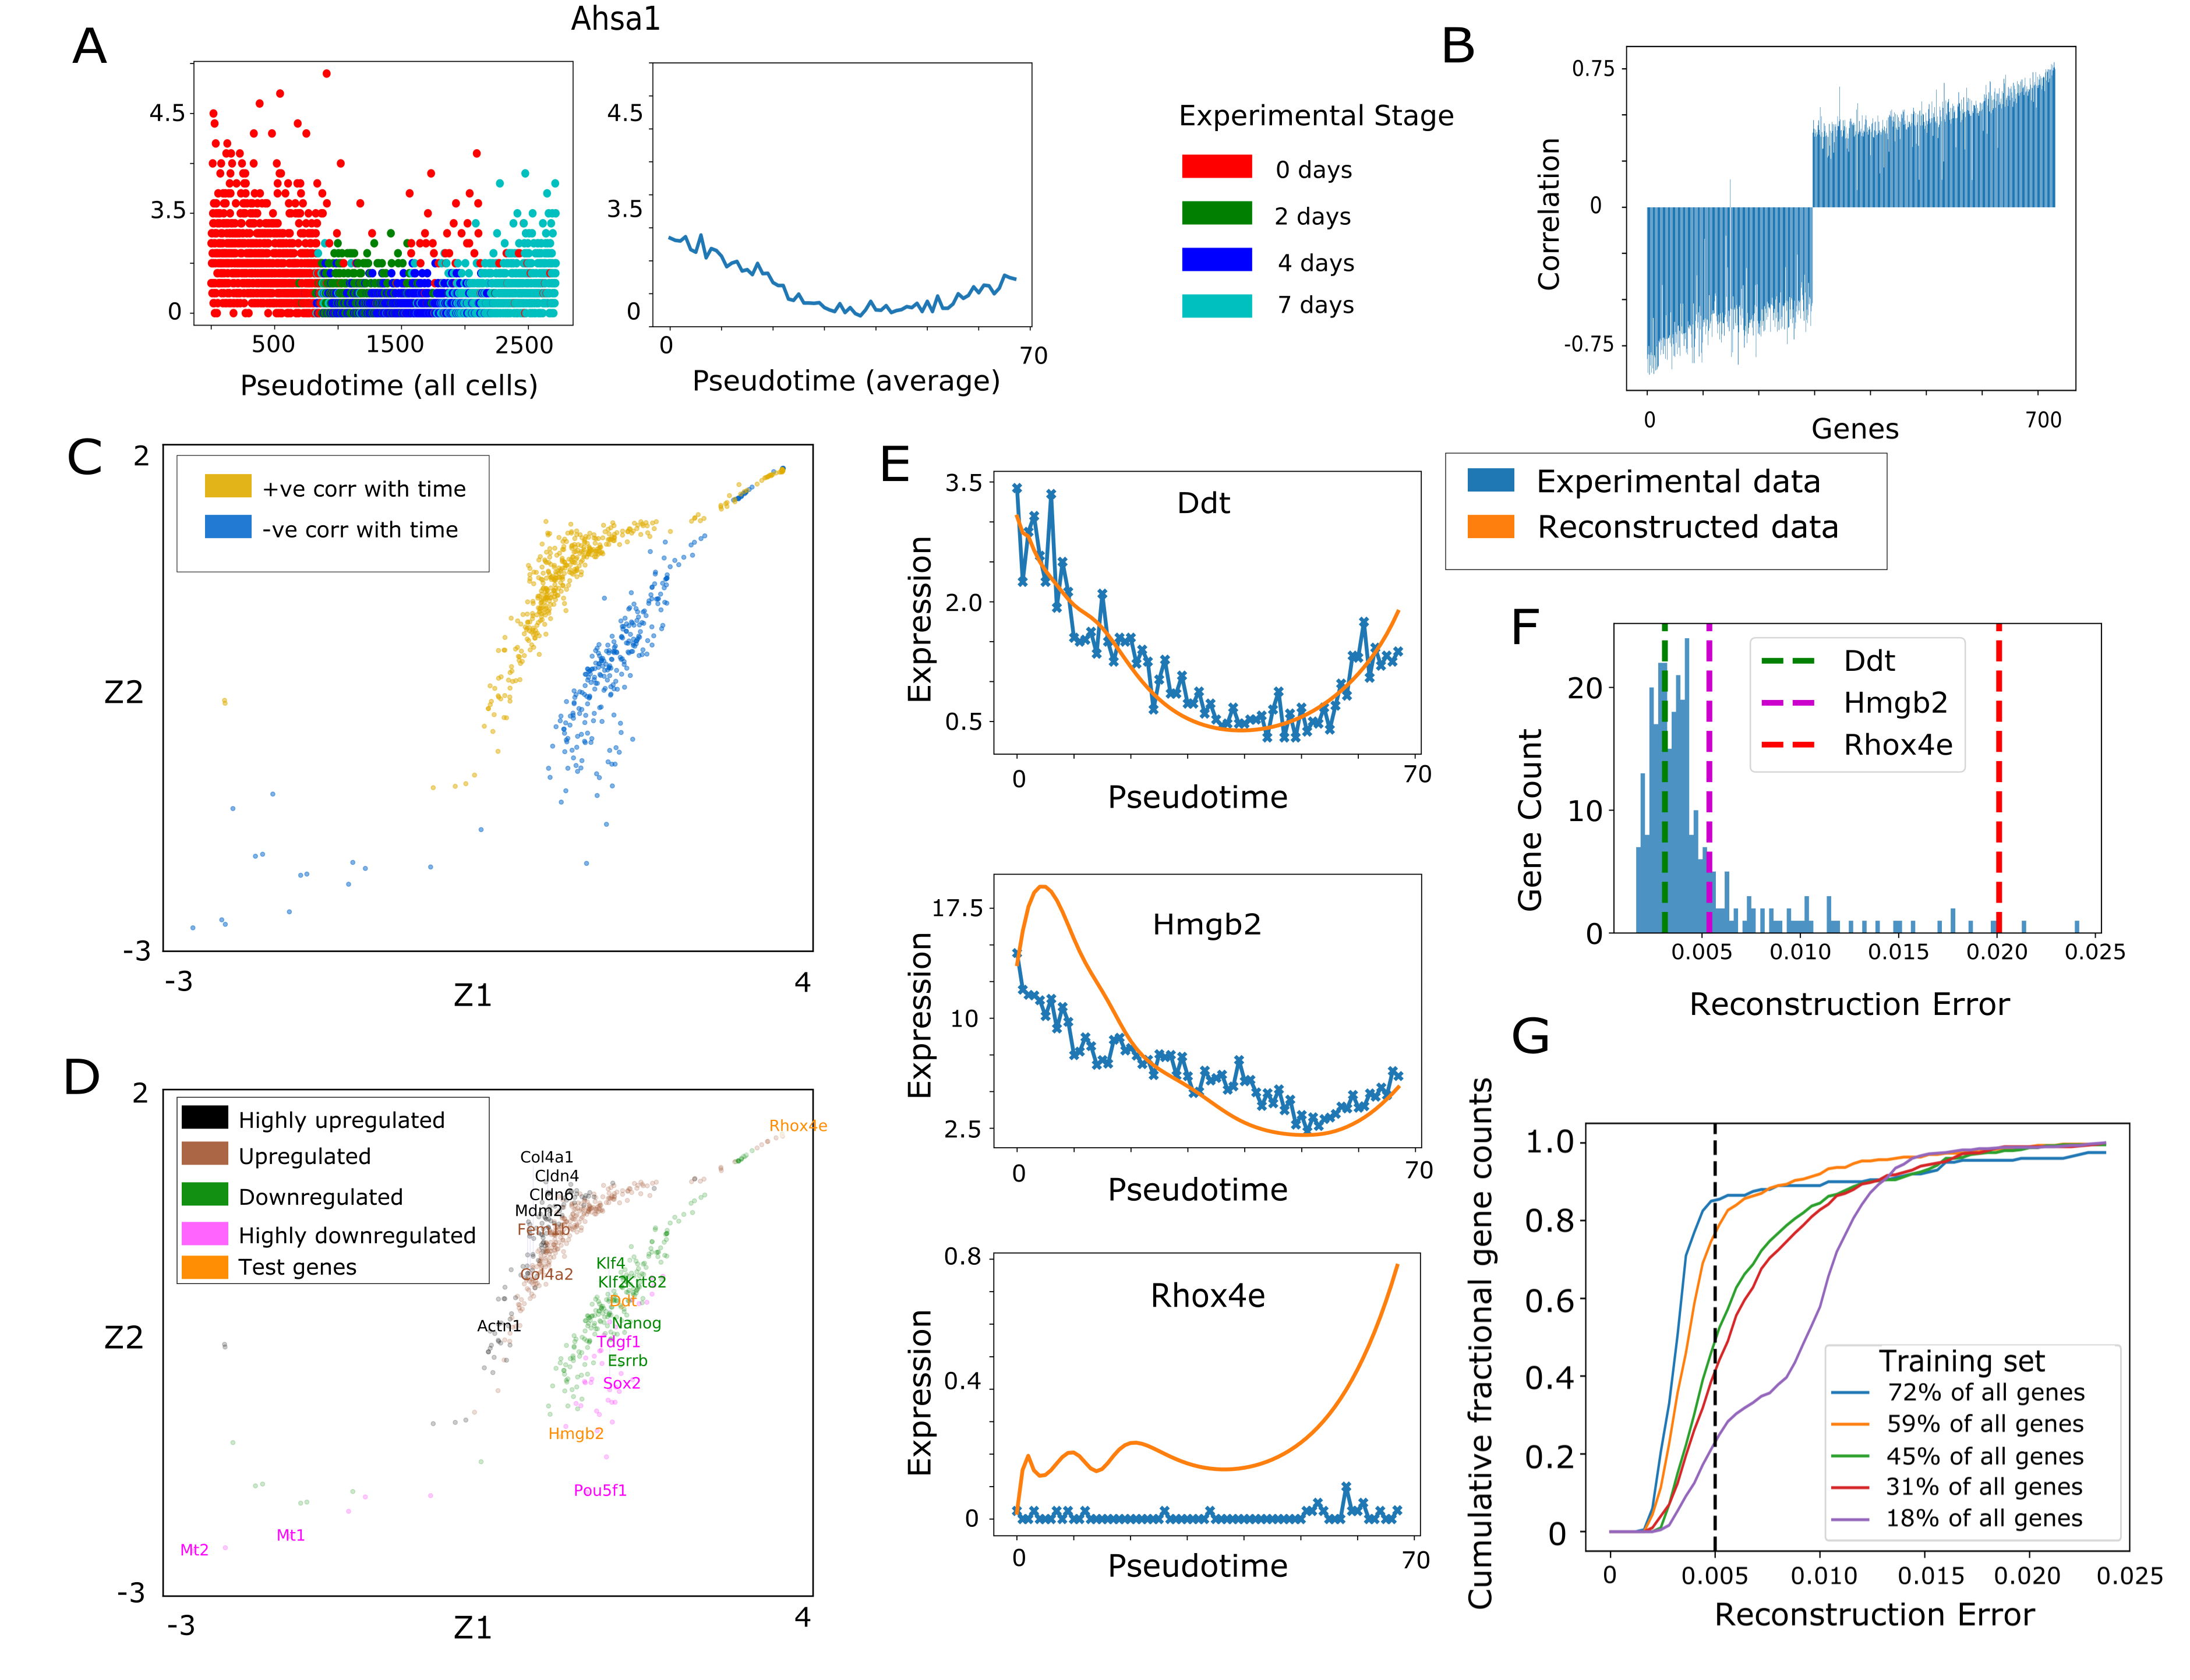
\includegraphics[width=\linewidth]{figures/esc_results.png}
 % archetecture.png: 1149x508 px, 72dpi, 40.53x17.92 cm, bb=0 0 1149 508
    \caption[Accurate reconstruction of embryonic stem cell differentiation dynamics with RVAgene.]{\textbf{Accurate reconstruction of embryonic stem cell differentiation dynamics with RVAgene.}
     ({\bf A}) Pseudotemporal ordering of 2717 single cells (data from \citep{Klein2015}), calculated using DPT; example gene shown: Ahsa1. Gene expression values given as log2(counts+1) for all cells (left), and for sliding window average (right).  ({\bf B}) Pearson correlation coefficient between gene expression and time for 732 differentially expressed genes.
    ({\bf C}) The 2D latent space learnt by an RVAgene model trained on 732 gene profiles over pseudotime, showing clear separation between upregulated and downregulated genes. ({\bf D}) Comparison of RVAgene and DPGP. The four largest clusters from DPGP are plotted on the RVAgene latent space: temporal expression patterns (from highly upregulated to highly downregulated) are in close agreement between methods. ({\bf E}) Comparison of experimental data and reconstructions. Model-generated reconstructions of three genes from the test set not used in training: Ddt, Hmgb2, and Rhox4e. Expression values are log2(counts+1).
    ({\bf F}) Distribution of average $L1$ reconstruction errors for the 300 genes used in the test set. Genes plotted in C are marked.
    ({\bf G}) Cumulative distributions of reconstruction errors on randomly sampled sets of test genes, where the full data were split into test groups of: 200 genes (train on 72\%), 300 genes (train on 59\%), 400 genes (train on 45\%), 500 genes (train on 31\%), and 600 genes (train on 18\%).}
    \label{fig:fig3}
\end{figure}
}

{\centering
\begin{figure}
  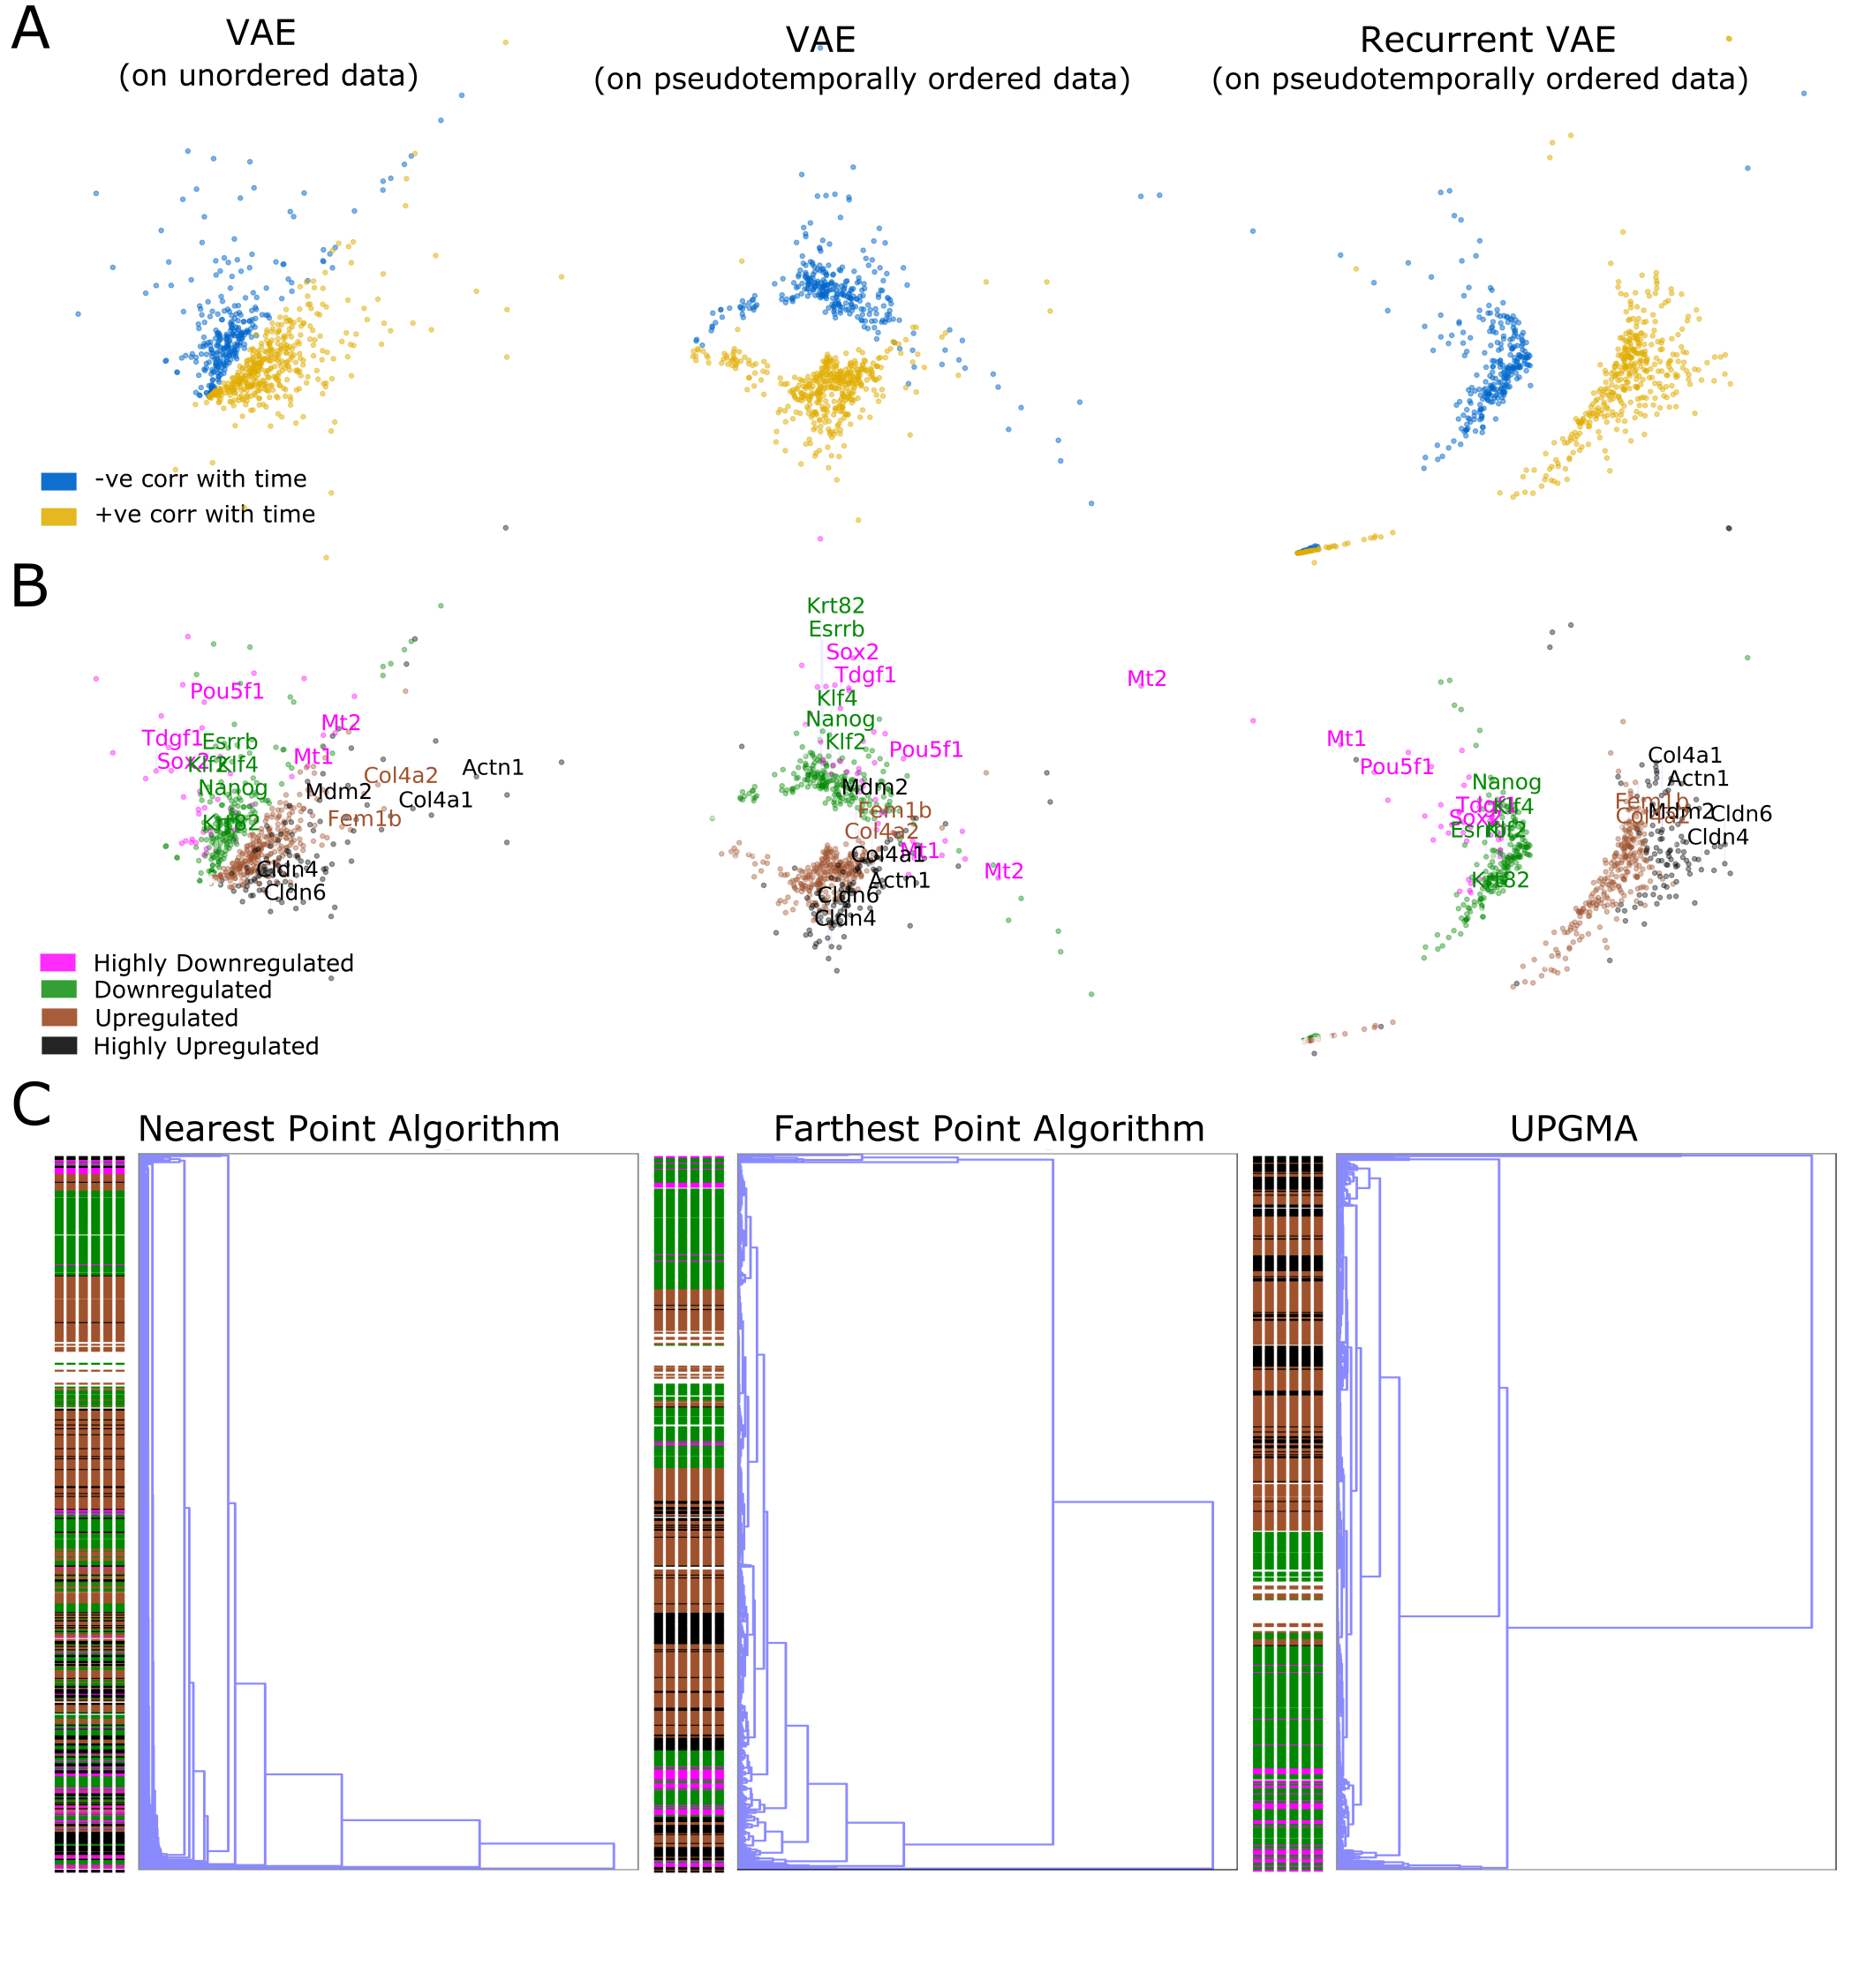
\includegraphics[width=\linewidth]{figures/vae_comp.png}
 % archetecture.png: 1149x508 px, 72dpi, 40.53x17.92 cm, bb=0 0 1149 508
    \caption[Comparison of information captured in RVAgene latent space compared to a standard fully connected VAE and results of standard hierarchical clusterings.]{\textbf{Comparison of information captured in RVAgene latent space compared to a standard fully connected VAE and results of standard hierarchical clusterings.}
    ({\bf A}) Here we show latent spaces learned by fully connected VAE and RVAgene. The pseudotemporally ordered data was also smoothed. ({\bf B}) We annotate the learned latent spaces using the top 4 clusters detected by DPGP on this dataset. In all three of these cases we report best results after relevant hyperparameter search and optimal training. ({\bf C}) We perform standard hierarchical clusterings (Nearest Point Algorithm, Farthest Point Algorithm and UPGMA (Unweighted Pair Group Method with Arithmetic mean) ) on pseudotemporally ordered and smoothed ESC data and annotate the learned representation in the same manner as in (B).} 
  \label{fig:fig4}
\end{figure}}

{
To assess the ability of the model to reconstruct genes not used during training, we kept aside 300 genes for testing and trained RVAgene on the remaining 432 genes.
We note that in this case (and in the case of single-cell datasets in general), the generative model of RVAgene produces pseudotime-smoothed gene expression trajectories, rather than being generative of raw pseudotemporal data, which tend to display overall high noise levels.
}
Reconstructed test gene expression profiles are shown for three reconstructed genes
(\hyperref[fig:fig3]{fig. 6.2E}), chosen to sample across the spectrum of reconstruction errors
(\hyperref[fig:fig3]{fig. 6.2F}). The reconstruction for {\em Ddt}, which has a reconstruction error
near the mode (\hyperref[fig:fig3]{fig. 6.2F}), shows very high accuracy. The reconstruction for
{\em Hmgb2}, which has twice the reconstruction error, still broadly captures the temporal profile
but with lesser accuracy. Finally we show the reconstruction for {\em Rhox4e}, a gene that was
sampled from the long tail of the reconstruction error distribution, i.e. does not well match the
data. Comparing these three examples with the full distribution of reconstruction errors
(\hyperref[fig:fig3]{fig. 6.2F}), we see that the large majority of genes lie to the left of {\em
Hmgb2}, i.e. have better-than-moderate accuracy. The reconstruction error of {\em Hmgb2} is close to
0.005, which we use as a cut off for ``well-reconstructed'' genes, based on analysis of individual
gene reconstructions. The cumulative reconstruction error distribution reiterates this point: 230
out of 300 genes (77\%) have a reconstruction error $\leq 0.005$ (\hyperref[fig:fig3]{fig. 6.2G}); we can conclude that the majority of test genes were faithfully reconstructed by the model.
\par
RVAgene accurately reconstructed most gene profiles using only $\sim60 {\%}$ of the data for
training (\hyperref[fig:fig3]{fig. 6.2G}), likely due to co-regulation of gene expression programs.
This led to a question: what is the smallest training gene set that can be used to accurately
reconstruct gene dynamics? We subset the data randomly into train/test sets and trained separate
RVAgene models on each. We found that reconstruction errors slowly increase as the size of the
training set decreases, but not until the training set was as low as $18\%$ of the data did the
reconstruction errors significantly increase (\hyperref[fig:fig3]{fig. 6.2G}, \hyperref[fig:figS4]{Fig. S19}). Analysis of the cumulative distribution of reconstruction errors across all groups found that RVAgene reconstructs the majority of gene temporal profiles well (defined as below a reconstruction error of 0.005) if $\geq 45\%$ of the data is used for training. The successful reconstruction of gene expression dynamics de novo while training on  small subsets of the data suggests widespread co-regulation of gene expression programs during embryonic stem cell differentiation, as found in previous work \citep{jang2017dynamics}.
% This information is a useful indicator to whether an algorithm estimating number of clusters is overfitting or underfitting (i.e. detecting too many or too few clusters), we talk about this in more detail later in \hyperref[discussion1]{Discussion} section. 

%{\centering
%\begin{figure}
%  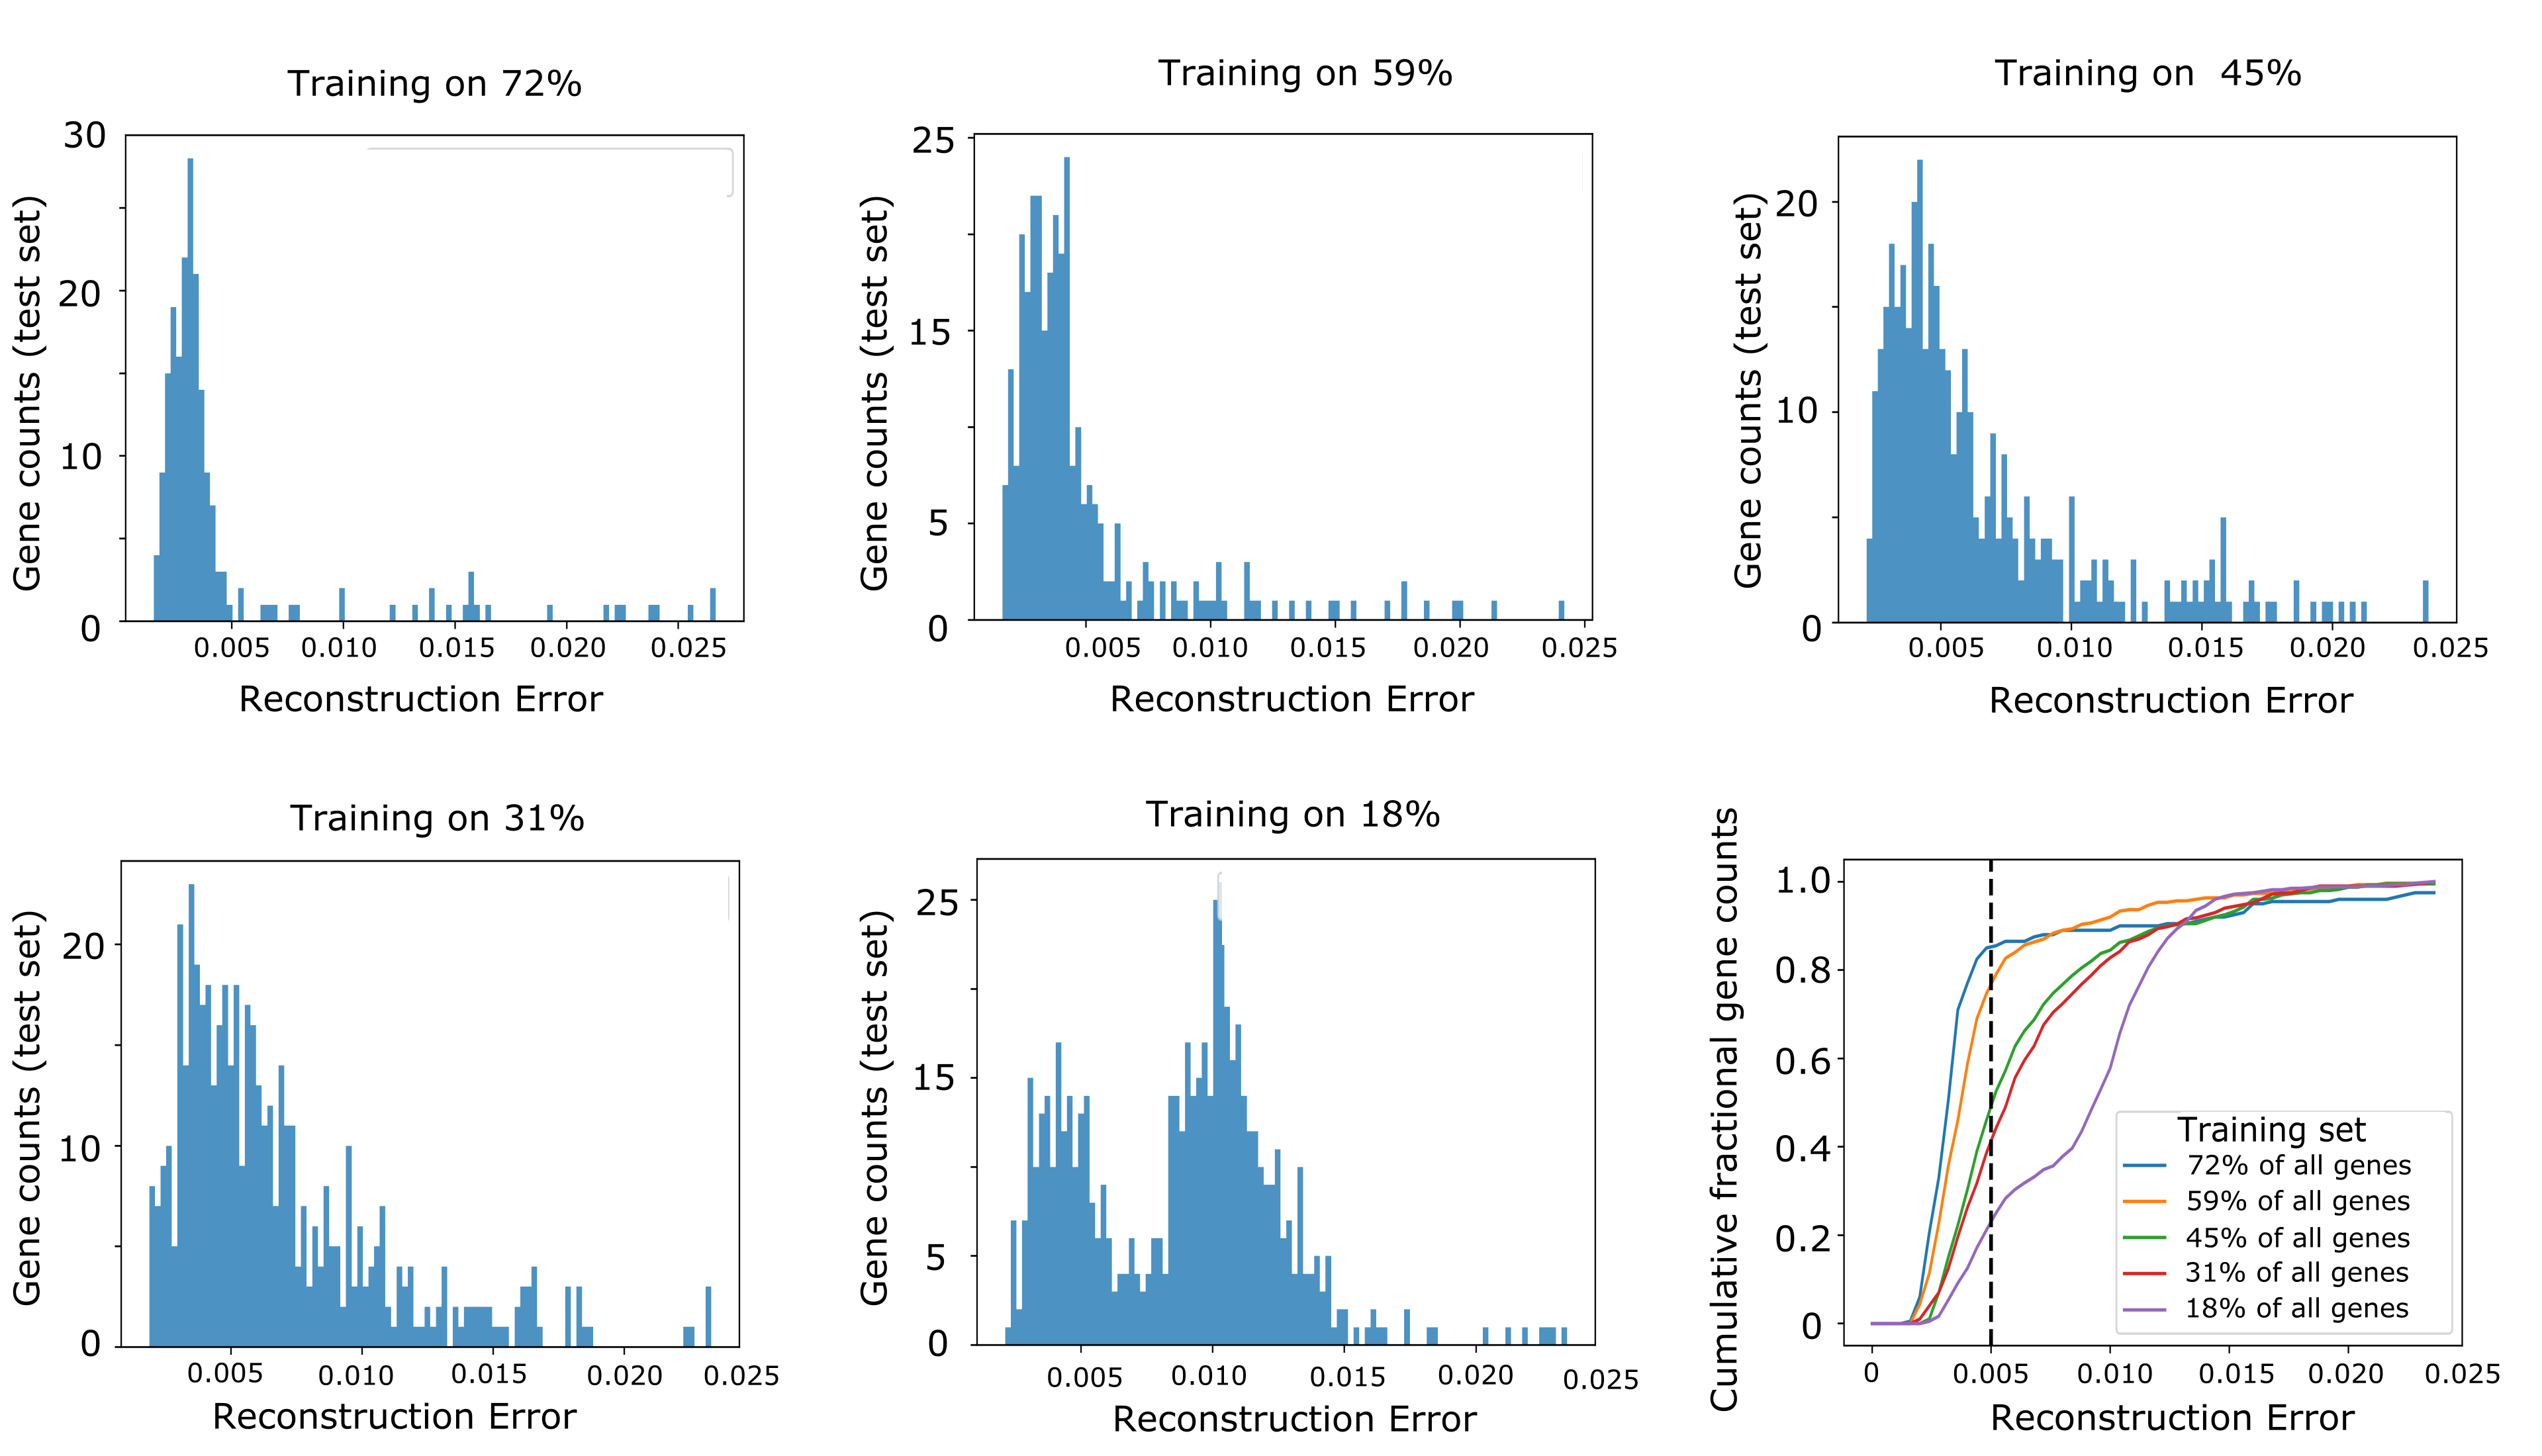
\includegraphics[width=\linewidth]{./figures/supp_varying_test_set_sizes.png}
 % archetecture.png: 1149x508 px, 72dpi, 40.53x17.92 cm, bb=0 0 1149 508
%    \caption{{\bf Accuracy of RVAgene reconstructions for different train/test group sizes.} Distributions of reconstruction errors on randomly sampled sets of test genes, where the full data were split into test groups of: 200 genes (train on 72\%), 300 genes (train on 59\%), 400 genes (train on 45\%), 500 genes (train on 31\%), and 600 genes (train on 18\%). Cumulative fractional distribution of reconstruction errors (cumulative count/test set size) for all groups.}
%  \label{fig:fig5}
%\end{figure}
%}


%\subsection{Comparison of RVAgene with alternative approaches for gene clustering}

In order to assess the performance of RVAgene for gene clustering and biological discovery, we compared it to five alternative methods: two neural network approaches and three hierarchical clustering methods. To assess the utility of the recurrent architecture of RVAgene, we trained non-recurrent (i.e. fully connected) variational autoencoders on the embryonic stem cell differentiation dataset \citep{Klein2015}. We compared two options: using the pseudotemporally ordered and smoothed data as input (same as for RVAgene), or using the raw (i.e. unordered and unsmoothed) gene expression data as input. We trained encoder and decoder networks of depth two (one hidden layer) and with a hidden layer size of 400 (we performed a hyperparameter search to optimize this). Theoretically, depth two networks are large enough to learn any non linear function \citep{cybenko1989approximation, hornik1989multilayer, funahashi1989approximate, barron1994approximation}, although the fully connected VAE has no recurrent inductive bias. Thus we test how important this recurrent inductive bias is in practice. 
\par 
The results of the comparison of neural networks are given in \hyperref[fig:fig4]{fig. 6.3A-B}. In
each case, models were trained for 200 epochs. Annotating the results in latent space using
correlations against pseudotime (\hyperref[fig:fig4]{fig. 6.3A}) shows that all three models
separate the data reasonably well, with slightly better separation for the recurrent architecture
(RVAgene). We also annotated the results using cluster labels from the largest four DPGP clusters
for comparison. These are appropriate ``gold-standard'' cluster labels since robust dynamical
signatures are learnt by DPGP in each case (\hyperref[fig:figS3]{Fig. S18}). RVAgene captures: 1) better
separation between clusters that either of the non-recurrent networks, and 2) a spectrum of
behaviors from up- to down-regulated (\hyperref[fig:fig4]{fig. 6.3B}).
\par 
We also performed hierarchical clustering on the pseudotemporally ordered and smoothed data using
three standard hierarchical clustering methods: the Nearest Point Algorithm, the Farthest Point
Algorithm, and UPGMA (the Unweighted Pair Group Method with Arithmetic mean). We annotated the
results with the same clusters labels from DPGP (\hyperref[fig:fig4]{fig. 6.3C}). UPGMA performs best out of these three clustering algorithms, yet still does not attain clear separation between each of the four groups. Thus, the 2D latent space representation of RVAgene is better than both 1D representations via hierarchical clustering and the alternative neural network latent space representations at distinguishing between dynamic gene profiles in pseudotemporally-ordered data.




%

{\centering
\begin{figure}
  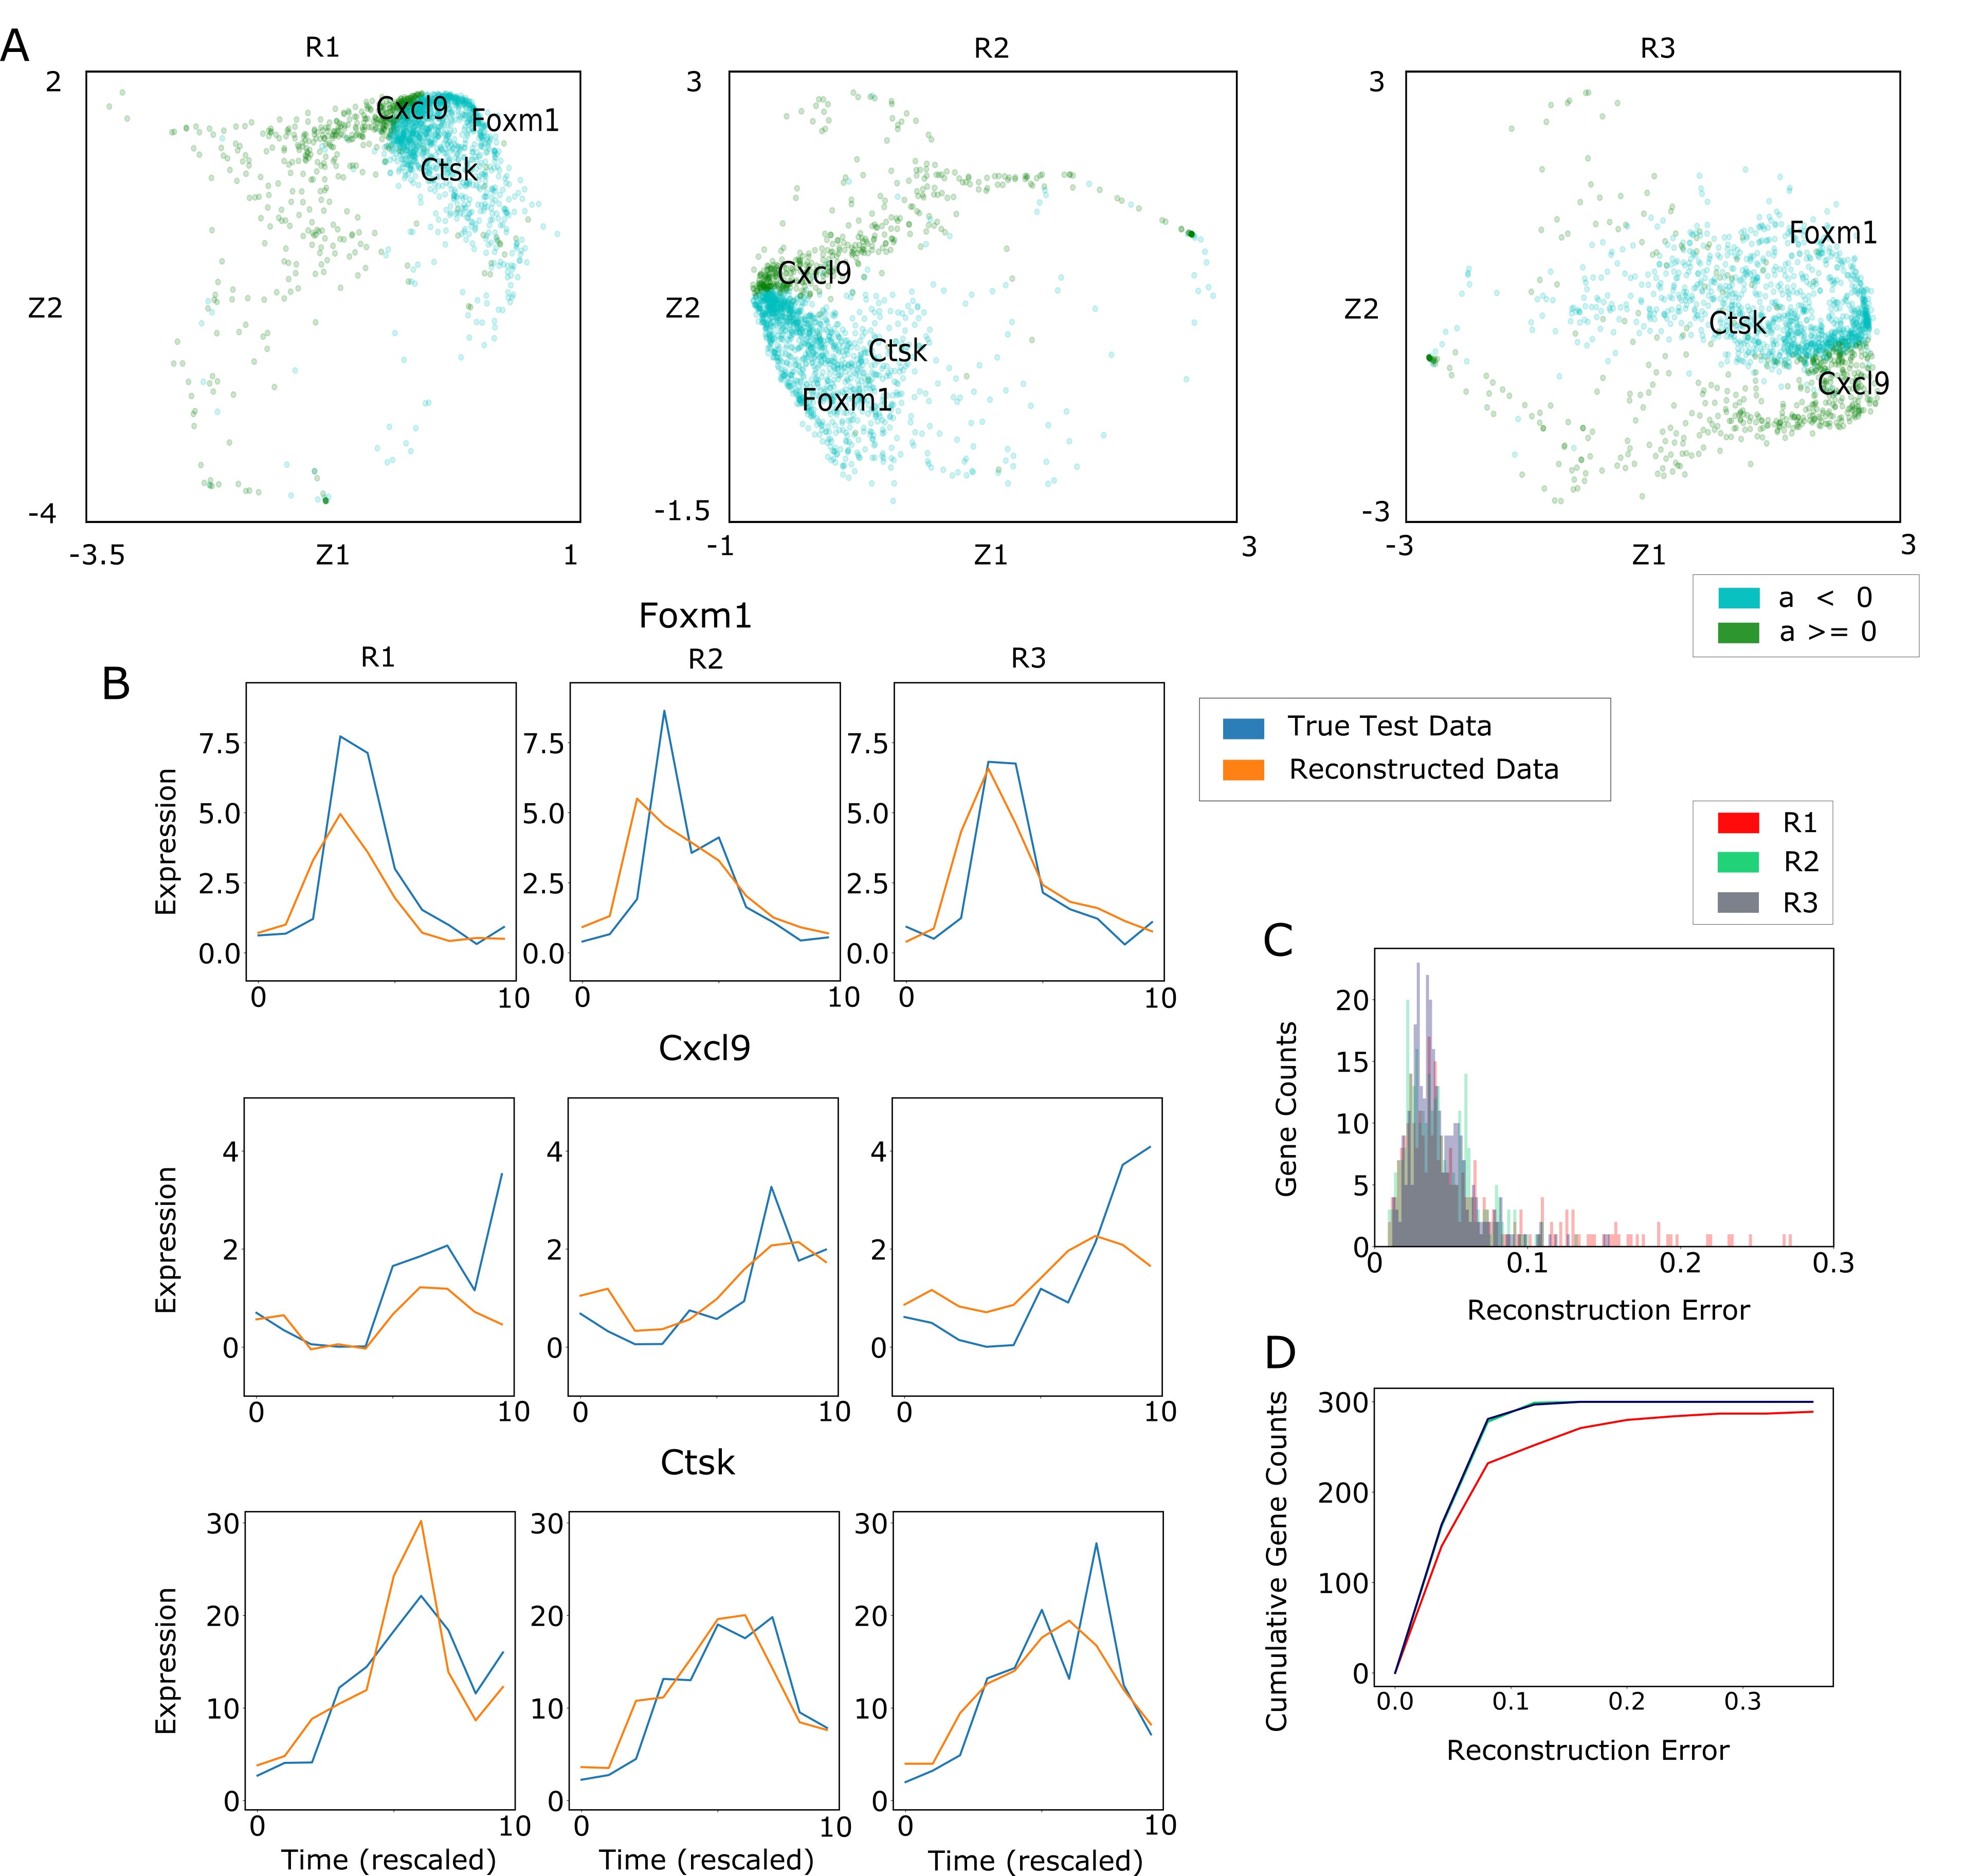
\includegraphics[width = \linewidth]{figures/quad_jci.png}
 % archetecture.png: 1149x508 px, 72dpi, 40.53x17.92 cm, bb=0 0 1149 508
    \caption[Accurate reconstruction of kidney injury response gene dynamics with RVAgene.]{{\bf Accurate reconstruction of kidney injury response gene dynamics with RVAgene. (A)} Latent space representations of RVAgene models trained separately on three independent replicates (R1-R3); classified by quadratic fit coefficient $a$. ({\bf B}) Model generation of gene dynamics for genes not used in training: {\em Foxm1, Cxcl9} and {\em Ctsk}. ({\bf C}) Histograms of reconstruction errors for RVAgene models trained on R1-R3 (truncated). ({\bf D}) Cumulative distribution of reconstruction errors. }
  \label{fig:fig6a}
\end{figure}
}



\subsection{RVAgene can classify and predict gene expression dynamics in response to kidney injury}

We investigated gene expression dynamics in the murine kidney by applying RVAgene to a dataset that describes gene expression profiles before, during, and after a kidney injury \citep{liu2017molecular}. The dataset is temporally rich, with a total of ten bulk samples over twelve months. Since in this case no single-cell information is available, we cannot order samples by pseudotime to smooth the data. Moreover, the temporal gene expression profiles described in \citet{liu2017molecular} display more complex dynamics than for the previous dataset \citep{Klein2015}, and are not readily separable by linear patterns of up- and down-regulated genes (cf. \hyperref[fig:fig3]{Fig. 2C}). Thus, below, we must consider nonlinear models in order to characterize the temporal patterns observed.
\par 
The data consist of one initial timepoint ($t = 0$) before the injury event (an ischemia/reperfusion injury model) and nine subsequent time points ($t = 1$ to $10$) following the injury (48 hours, 72 hours, 7 days, 14 days, 28 days, 6 months and 12 months). We note that the timepoints are not uniformly spaced, which is not taken into account in RVAgene, which only models the broad temporal trend (see Discussion). From an initial list of 1927 differentially expressed genes measured over the time course in three biological replicates, we removed putative/predicted and non-protein coding genes, retaining a list of 1713 genes as input to the model.
\par 
We ran RVAgene separately for each of three biological replicates. Independent replicates \& independently trained models provide additional means with which to test the reproducibility of these methods. For each replicate, RVAgene was trained with a two-dimensional latent space and a hidden size of 10, on the full set of genes over 200 epochs: found to be sufficient for the convergence of $\cL$ (see Methods for further details). We fit linear regression models to the temporal gene profiles (\hyperref[supp]{Fig. S5}) and found that linear fits rarely described the gene temporal profiles well (most correlation coefficients had values close to zero), not did they identify separate clusters in the latent space. Normalizing the data to lie in $[0,1]$ improved our ability to discriminate clusters in the latent space (\hyperref[supp]{Fig. S5C}), but came at the expense of a significant loss of information, as the variance captured in the latent space was dramatically reduced. The absence of evidence for linear correlations could indicate expression dynamics that are uncorrelated with time, but could of course also indicate more complicated (nonlinear) gene expression dynamics, which are explored below. 
\par
To study nonlinear gene expression dynamics, we fit a 2nd degree polynomial, i.e. we fit the temporal trajectory of each gene $x$ to:  $x = at^2 + bt + c$, where $a,b,c$ are constants (\hyperref[supp]{Fig. S6}). We hypothesized that this function could adequately describe the transient dynamics observed by \citet{liu2017molecular} for most genes in response to the kidney injury. 
% Our hypothesis was that this model would be sufficient to capture simple patterns commonly observed during and following kidney injury, where the expression of a gene either increases or decreases transiently, before returning to near-baseline expression values.
Thus, we classified genes into one of two groups, $a < 0$: convex (up-down pattern), 1200 genes; and $a \geq 0$: concave (down-up pattern), 512 genes. In the latent space, the separation of these two groups is clearly visible for each replicate (\hyperref[fig:fig6a]{Fig. 4A}). Moreover, the classification is in agreement with \citet{liu2017molecular}, where the majority of differentially expressed genes are upregulated transiently. 
To explore the ability of RVAgene to reconstruct gene expression profiles not used in model development, we kept aside 300 randomly sampled genes for testing, and trained RVAgene models on the remaining genes for each of the three replicates. Independently for each model, we then generated dynamic profiles for the test genes. Three genes sampled randomly from the test set are plotted in \hyperref[fig:fig6a]{Fig. 4B}. Of particular note, for each of genes, the model-generated data captures the temporal patterns while displaying a higher degree of similarity across replicates than the experimental data itself. This illustrates that the model is neither under- nor overfitting, but capturing the underlying biological patterns while sufficiently accounting for the noise. 
%An interesting point to note is that for each of the shown example genes, the three separately trained RVAgene models for the three replicates come up with similar looking reconstructions although the actual data of the three replicates have different variations (while conforming with the general dynamics common to the three replicates).
Reconstruction errors are comparable across the three replicates, albeit with slightly higher overall errors in replicate 1 (\hyperref[fig:fig6a]{Fig. 4C-D}). Overall, the reconstruction errors are higher than for the previous section (averaging over many pseudotemporal time points allowed us to significantly reduced the noise). 



{\centering
\begin{figure}
  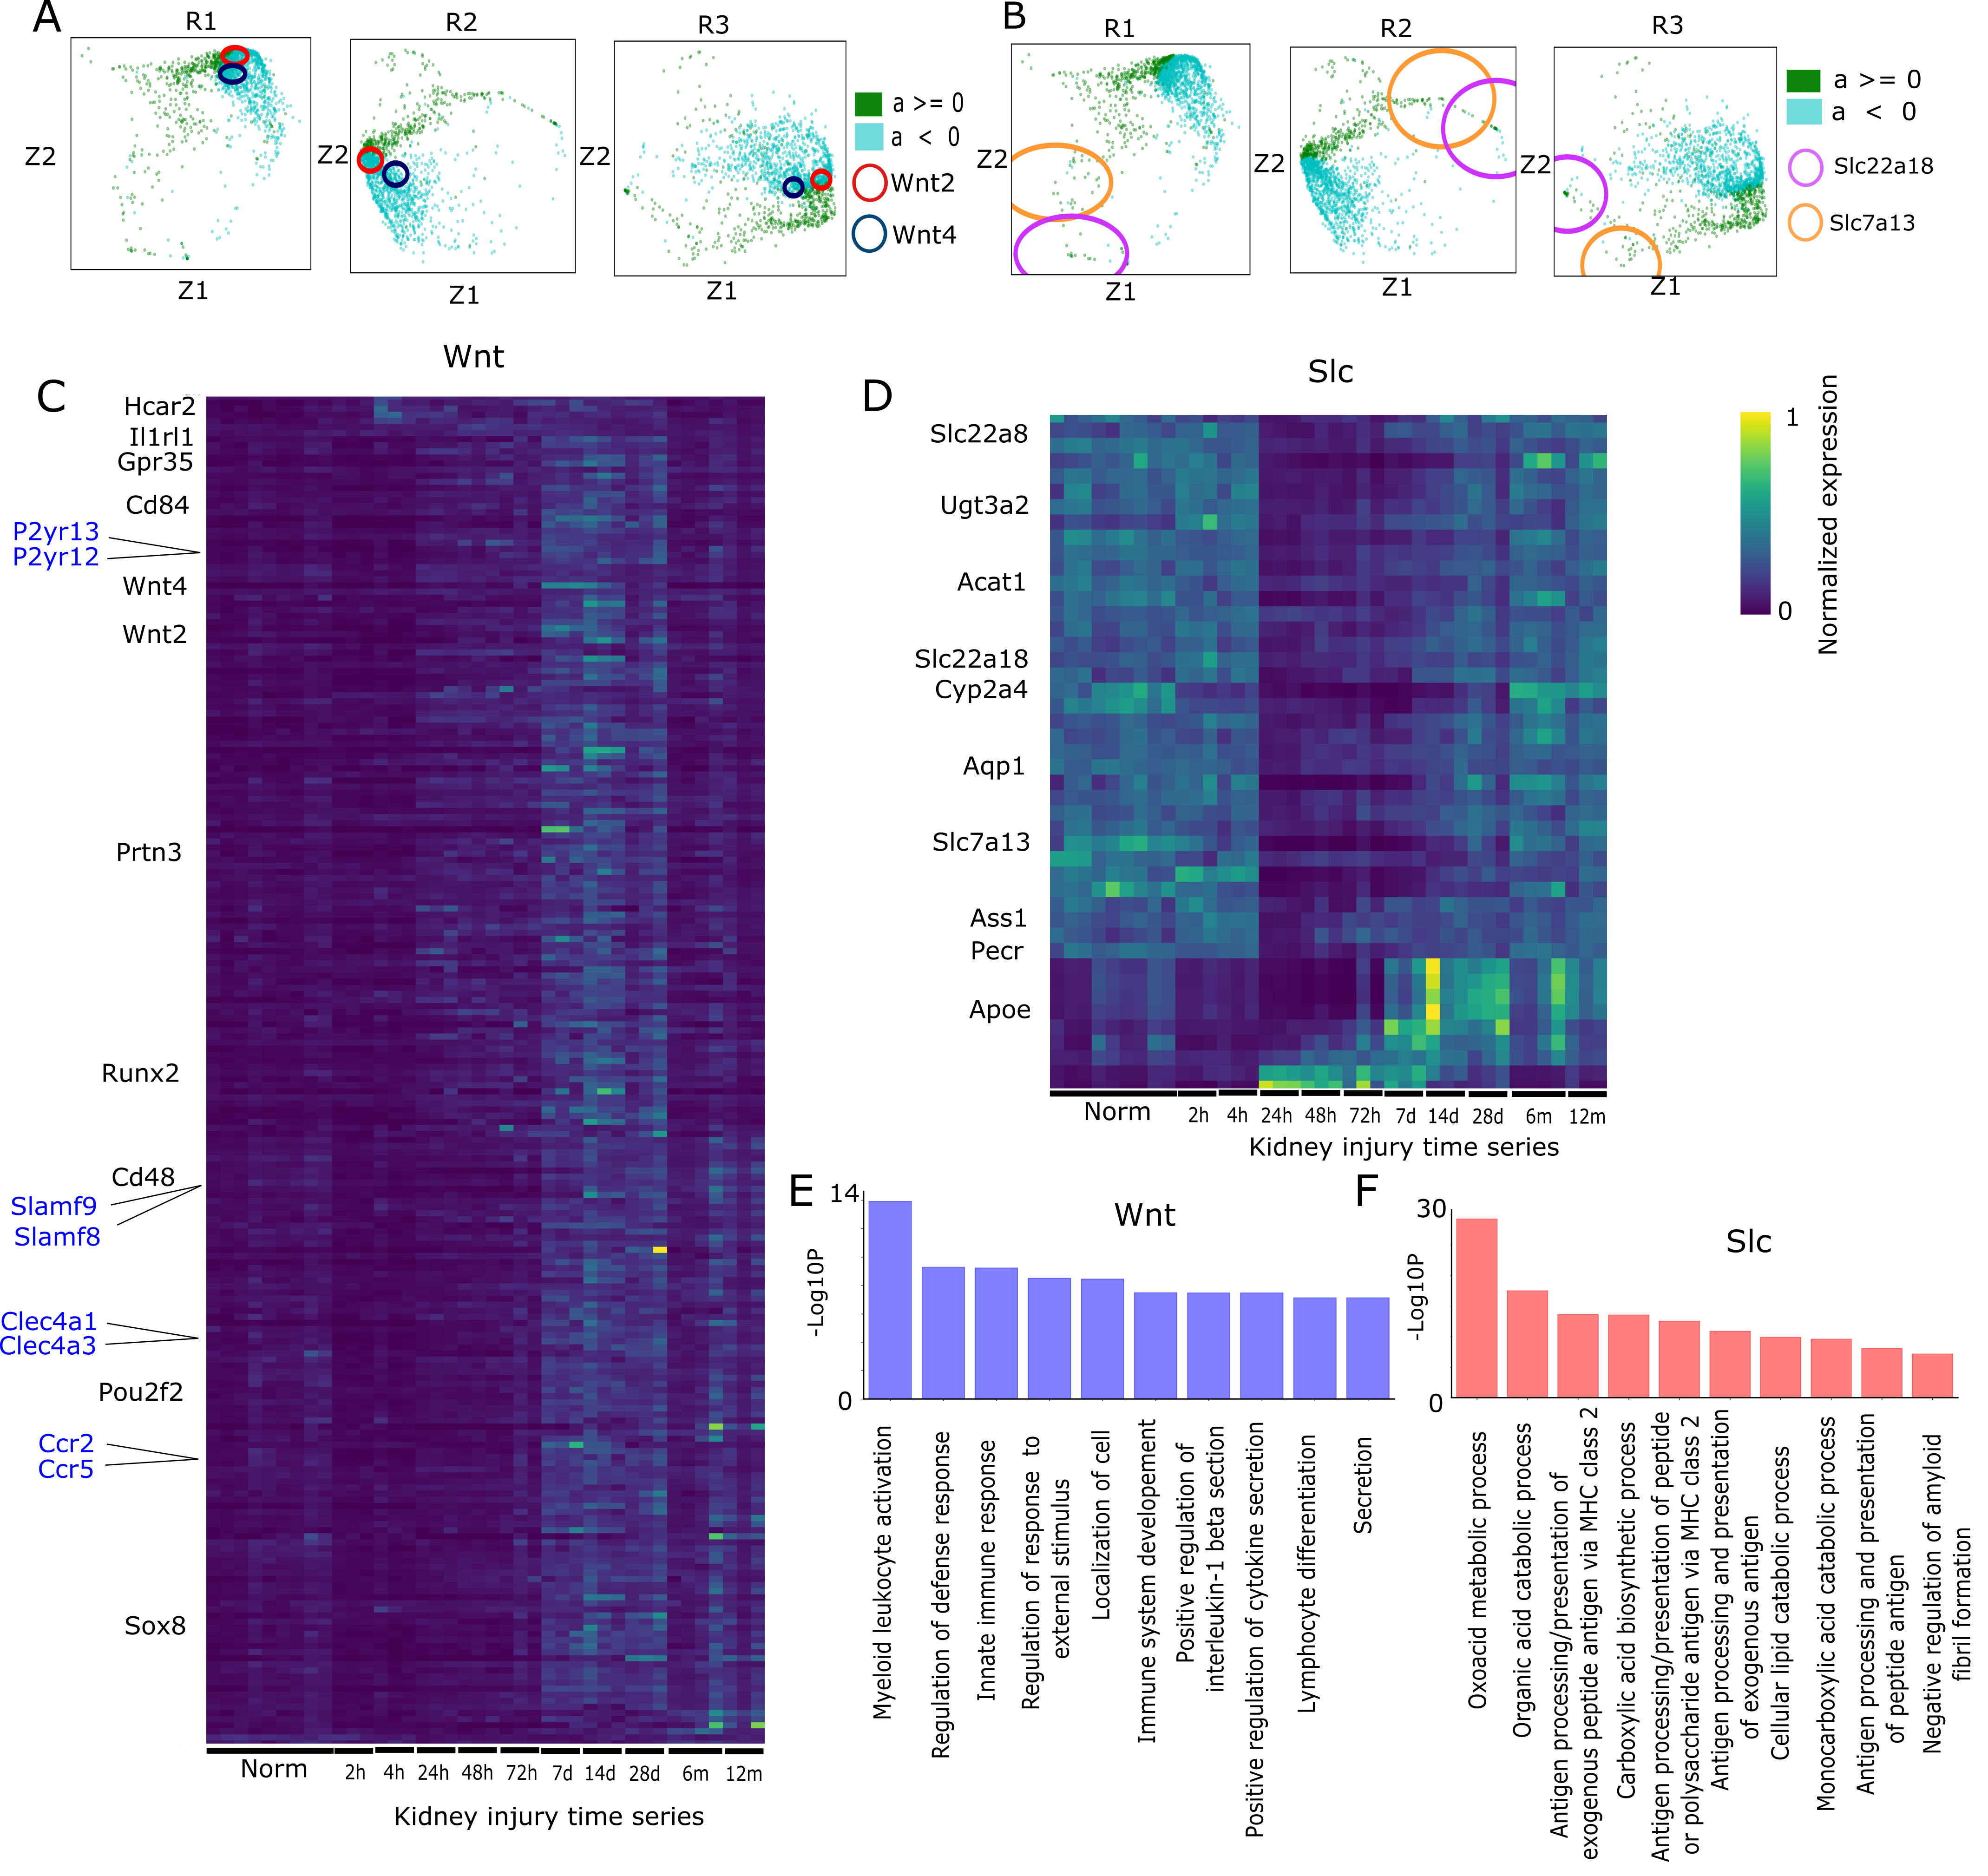
\includegraphics[width = \linewidth]{figures/fig9.png}
 % archetecture.png: 1149x508 px, 72dpi, 40.53x17.92 cm, bb=0 0 1149 508
    \caption[RVAgene latent space captures biological processes driving concordant gene expression changes.]{{\bf RVAgene latent space captures biological processes driving concordant gene expression changes. (A)} Z-plots for replicates R1-R3 with local neighborhoods of Wnt2 and Wnt4 marked (circles). ({\bf B}) As in A, for Slc family members Slc22a18 and Slc7a13. ({\bf C}) Heatmap of expression changes over time course of injury for the Wnt neighborhood genes in the intersection of R1-R3. Selected genes marked (black), as well as ortholog gene pairs (blue).  ({\bf D}) As in C, for Slc neighborhood genes. ({\bf E}) Histogram of -log10 p values of gene ontology terms for biological processes terms associated with the Wnt neighborhood (gene set in C). ({\bf F}) As in E, with the Slc neighborhood (gene set in D). }
  \label{fig:fig6b}
\end{figure}
}

{
  To investigate in more depth the features that are captured in the RVAgene latent space, we performed two sets of analyses: unbiased clustering, and targeted exploration. For the unbiased analysis, we performed k-means clustering on RVAgene latent space of replicate 1 (R1) with $k=9$ (Supplementary \hyperref[supp]{Fig. S7A}); we project the clusters labels learnt onto replicates R2 and R3. All cluster identities are well-preserved across replicates, with the exception of cluster 5, which seems to indicate outlier genes in R1. To study biological processes within these clusters, we performed GO term enrichment analysis on each. In Supplementary  \hyperref[supp]{Fig. S7B} we plot one significant GO term per cluster (omitting cluster 5), and see that specific regions of the latent spaces across replicates can be characterized in terms of biological processes, many of which relate to metabolic and immune system responses. These can be separated into two broad classes, which separate the left-hand side of R1 (metabolic processes downregulated during injury response) from the right-hand side (immune responses upregulated during injury response). 
}
\par 
To study the effects of gene-specific regions of the latent space in greater depth, we chose three distinct regions based on the co-location of genes of interest. These gene groups studied on the latent space are: 1) a {\em Wnt} group consisting of family members {\em Wnt2} \& {\em Wnt4}; 2) an {\em Slc} group consisting of family members {\em Slc7a13} \& {\em Slc22a18}; and 3) a {\em Sdc1} group, consisting of only {\em Sdc1}. For each group, we characterized neighboring genes by defining a circular neighborhood around each gene in the group, with radius $r$ (depending on the local density, the radius was varied, giving: $r^2 = 1$ for {\em Slc}, $r^2 = 0.3$ for {\em Sdc}, $r^2 = 0.05$ for {\em Wnt}. We then took all genes inside this radius for each replicate, and found the intersection of genes over the three replicates (\hyperref[fig:fig6b]{Fig. 5A-B}). We analyzed the intersection gene set for each group by studying their temporal profiles and their gene ontology (GO) term associations. Each group was characterized by a strikingly clear temporal profile. The {\em Sdc1} and {\em Wnt} groups both show transient upregulation, over different timescales: the {\em Sdc1} group is upregulated from 24 hours post-injury until 14-28 days post-injury (fast response) (Supplementary \hyperref[supp]{Fig. S8B}), whereas the {\em Wnt} group is upregulated at 7 days post-injury until 28 days post-injury (slow response) (\hyperref[fig:fig6b]{Fig. 5C}). In contrast, the {\em Slc} group is downregulated at 24 hours post-injury, and remains suppressed until 7-28 days post-injury (\hyperref[fig:fig6b]{Fig. 5D}).
\par 
Analysis of GO biological process terms enriched in each gene group further highlighted the power of the latent space for biological discovery. The fast response ({\em Sdc1}) group was characterized by upregulation of programs related to apoptosis, stress response, wound healing and chemotaxis, i.e. the first responders to the site of injury (\hyperref[supp]{Fig. S8C}). In addition all five {\em Lox} genes comprising the GO term ``peptidyl-lysine oxidization'' were found in this group. This is consistent with the oxidative stress resulting from the renal ischemia-reperfusion injury that was performed. However, distinct factors regulate the {\em Lox} family genes, as can be partly observed by their subtle differences in temporal profile (\hyperref[supp]{Fig. S8D}). Their co-location in the latent spaces of all three models thus highlights the potential use of RVAgene for discovery of complex temporal regulatory events from gene expression data.
\par
The slow response ({\em Wnt}) group was primarily characterized by immune response processes, including leukocyte activation, platelet aggregation, and various cytokine-mediated pathways including {\em IL-1} and {\em IL-33} (\hyperref[fig:fig6b]{Fig. 5E}). Notably, the Wnt group identies multiple gene orthologs (\hyperref[fig:fig6b]{Fig. 5C}) with very similar profiles: likely evidence of shared temporal regulation. This illustrates once again (as for the {\em Lox} genes above) the potency of RVAgene for the discovery of temporally co-regulated genes.
\par
Finally, the {\em Slc} group of genes shows a transiently down-regulated pattern between 24 hours and 7-28 days, although some gene in this group deviate from this pattern (\hyperref[fig:fig6b]{Fig. 5D}). 
GO term enrichment identifies the positive regulation of metabolic processes (\hyperref[fig:fig6b]{Fig. 5F}). The downregulation of metabolic programs during the response to kidney injury is agreement with the findings of \citet{liu2017molecular}. Notably, this metabolism-sensitive group contains many genes that also display sexually dimorphic expression, primarily in specific regions of the proximal tubule \citep{ransick19_singlecell}, thus independently identifying the well-established (though under-studied) interplay between sex differences and injury responses in the kidney \citep{neugarten00_effect}. 
\par 
In summary, unsupervised analysis of groups of genes co-located in the latent spaces of RVAgene finds: 1) high similarity between temporal gene profiles of genes nearby in latent space, and 2) clear biological signatures represented by these groups of nearby genes, in strong agreement with prior knowledge \citep{liu2017molecular}. Moreover, the latent spaces of RVAgene models can be used to predict programs of temporal co-regulation. 
\par


% In the latent space representation for all those genes and for the three replicates. We can see genes with positive and negative correlation between expression and time axis are not as distinctly separated as previous section, which is expected (Supplementary \hyperref[supp]{Fig. S2-B}). 
% This also hints that this dataset might not have clear cluster structures and an uninformed clustering effort on this dataset might produce forced spurious results. Now, one might think that the correlation measure is a measure of shape and somehow magnitude of expression of genes is playing part here (i.e. may be genes with similar dynamics but different scale of magnitudes are being viewed differently). Which means, normalising the expression magnitudes across timepoints to the same range (e.g. 0-1) might be helpful to increase the clarity of separation between the red and blue class. This indeed works as can be seen in supplementary \hyperref[supp]{Fig. S2-C}. However, it drastically reduces the variance in the latent space which can be inferred from the hugely shrunken scales of the axes from supplementary \hyperref[supp]{Fig. S2-B} to supplementary \hyperref[supp]{Fig. S2-C} for both dimensions of latent space i.e. a lot of important information is lost. This might not be a problem for the representation learning part, but, it means the decoder will be hugely underfit. So, we do not recommend normalising the data without any solid reason for the same. Another possibility is increasing the dimension of latent space. A 3D latent space could be better in this case but increasing it beyond 3 defeats the purpose of representation learning because each gene has only 10 timepoints anyway and latent space with more than 3 dimension will require dimensionality reduction for visualization.
 
%%% Local Variables:
%%% mode: latex
%%% TeX-master: t
%%% End:

%
\begin{center}
    \begin{figure}
    \makebox[\textwidth]{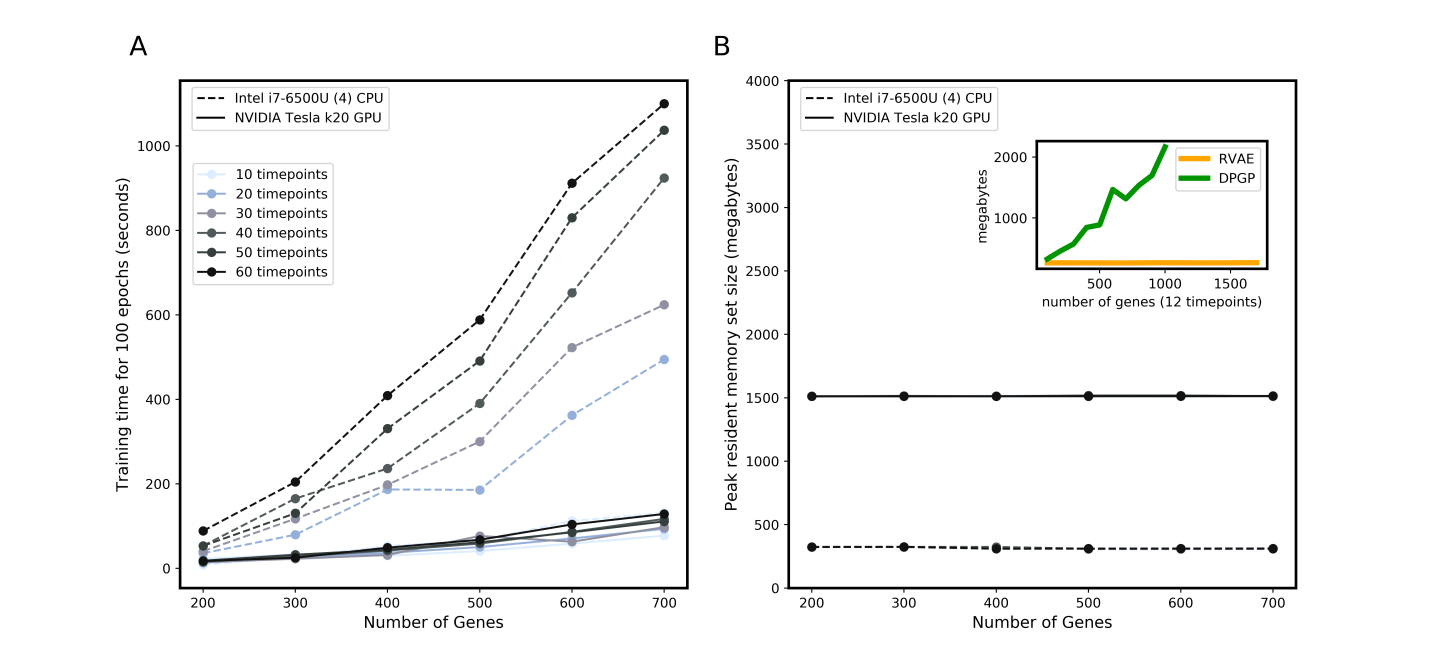
\includegraphics[width=0.8\paperwidth]{figures/fig7.png}}
 % archetecture.png: 1149x508 px, 72dpi, 40.53x17.92 cm, bb=0 0 1149 508
        \caption[Computational cost of training RVAgene]{\textbf{Training RVAgene is reasonably scalable on CPU and even more so using hardware acceleration through GPU.} ({\bf A}) Time cost of training RVAgene for 100 epochs for datasets with varying number of genes and time points on CPU and GPU. ({\bf B}) Maximum memory utilized during training of the model on CPU an GPU for the cases in (A), inset plot: comparison of max memory used compared to DPGP for varying number of genes.}
  \label{fig:fig7}
\end{figure}
\end{center}


\subsection{Assessment of the computational efficiency of RVAgene}

We assessed the computational efficiency of RVAgene for various settings and hardware. For the
majority of the models trained, 100-200 epochs was sufficient for the loss function $\cL$ to
converge. For tests performed here, we recorded the RVAgene runtime for 100 epochs of training using
models that varied in their number of genes and time points. In each case we used a latent space of
dimension two, a hidden size of 10, and a training batch size of 10. We ran the model on an intel i7
CPU with four cores and a Tesla K20 GPU. Runtimes were recorded on linux via the inbuilt time script
(\texttt{/usr/bin/time --verbose}). As the number of time points and genes grew large (up to 60 time
points and 700 genes), total runtimes on CPU were on the order of $10^3$ seconds ($<$ 20 minutes)
(\hyperref[fig:fig7]{fig. 6.6A}). On GPU, total runtimes were decreased to around $100$ seconds ($< 3$ minutes). Thus, RVAgene is readily scalable to tens of thousands of genes and hundreds of time points for training times of up to a few days on CPU or hours on GPU. For comparison, as described in \citet{McDowell2018}, the approximation-free time complexity of each iteration of learning for DPGP is $\cO(GT^3)$, due to the $G$ matrix inversions, each of size $T \times T$, for a dataset with $G$ genes and $T$ timepoints. The complexity for each epoch of training of RVAgene is $\cO(GT)$.
%The cubic complexity of the hierarchical Gaussian Process learning in DPGP quickly increases training time and does not allow scalability over timepoints without some form of approximation.
\par 
In terms of peak memory usage, since RVAgene is a neural network trained using backpropagation
\citep{rumelhart1986learning}, maximum memory used during training is of the same size as the
network itself, which is constant given that the model parameters are fixed
(\hyperref[fig:fig7]{fig. 6.6B}). This is in contrast to Gaussian Processes (such as DPGP), which
initially assign each gene to its own cluster, thus must store $G$ matrices of size $T\times T $,
for $G$ genes and $T$ timepoints per gene. This leads to quickly increasing runtime peak resident
set sizes for DPGP compared to RVAgene (\hyperref[fig:fig7]{fig. 6.6B} Inset). The memory used by DPGP grows with the number of time points as $\cO(GT^2)$). Thus, DPGP will not run with large numbers of genes and time points. %, and RVAgene has greater potential for the discovery of nuanced dynamical features in the data.
A note on this comparison: it is not direct, in the sense that DPGP performs clustering and RVAgene does not, in addition to other important differences between the goals of the methods. 
%However, we must add that direct comparisons must be made cautiously, given the differences between the two methods. 
%DPGP performs independent gene clustering; RVAgene does not (clustering can be performed downstream on the latent space).
Nonetheless, the size and scope of current biological datasets -- particularly at single-cell resolution -- in many cases preclude the use of DPGP without large reductions of the input data size. As we have shown, a feasible and efficient alternative in such cases is to run RVAgene, and then to perform clustering or other classification analyses post hoc on the latent space of the model. 


%%what does it do?
%- visualization/classification (encoder) and prediction/generation (decoder)
%
%Plan
%- overview of main findings - ability to classify, predict, and generate 
%- current uses - tuning hyperparameters (DPGP) 
%- current uses - interpretability (cf. other VAEs)
%- future uses - interpretability - using LDVAE
%- future uses - (GRNs)
%- future work: time interval 
%- future work: discret time 
%- future work: different priors (cite SOUP)
%- conclusion


\section{Discussion}
{We have presented RVAgene, a recurrent variational autoencoder for generative modeling of gene expression time series data.
Through its encoder network, RVAgene provides means to visualize and classify gene expression dynamic profiles, which can lead to the discovery of biological processes.
Through its decoder network, RVAgene provides means to generate new gene expression dynamic profiles of either the full data or (in the case of single-cell studies) the pseudotime-smoothed data by sampling points from the latent space. In doing so, RVAgene can accurately reconstruct gene dynamics in complex biological data. As a by-product, on single-cell datasets the model directly produces smoothed outputs, useful for denoising gene expression time series data. RVAgene is efficient on temporally-rich whole genome datasets, in comparison to current existing methods. }
\par
RVAgene can be used to discover structure in the data, such as gene profile clusters. Popular
methods for clustering gene profiles such as Bayesian hierarchical clustering
\citep{cooke2011bayesian} or DPGP \citep{McDowell2018} detect the number of clusters in the data by
fitting a hyperparameter $\alpha$, the concentration parameter of the governing Dirichlet process
\citep{ferguson1973bayesian}. Although unsupervised, inevitably, the choice of $\alpha$ affects the
number of clusters output. Visualizing the data first with RVAgene can give an idea whether the data
favor clustering or a continuous representation. Thus analysis in RVAgene can guide the setting of
the hyperparameter $\alpha$ in DPGP and similar methods. In the case of ESC differentiation, DPGP
predicts 12 clusters (\hyperref[supp]{ Fig. S3}), yet most have very few members and many share
similar patterns. The RVAgene latent space for this dataset finds two major divisions in the data,
and orders the largest DPGP clusters along a spectrum (\hyperref[fig:fig3]{Fig. 1.2D}), suggesting that DPGP might be overfitting the data. Indeed, the two methods can be used complementarily: RVAgene for high-level structure discovery and DPGP for clustering.
{In cases where learning a detailed noise model (at single time point resolution) is important to the user, DPGP or other Gaussian Process models are preferable over RVAgene.}
However, DPGP does not scale well with large datasets and thus cannot always be used
(\hyperref[fig:fig7]{Fig. 1.6}).
\par 
The latent space of an RVAgene model encodes useful information about biological features, and in that sense provides biologically interpretable representations of the data. However, the representation is not interpretable in the sense that the components of the latent space do not have a physical meaning nor are they necessarily independent. Recent methods have tackled this issue of interpretability, by either modifying the loss function to make components independent \citep{higgins2016beta} or substituting linear functions in parts of the VAE \citep{svensson2020interpretable, ainsworth2018oi}. These methods have clear advantages regarding the analysis and interpretation of features in the latent space. In future work, decoding an RVAgene model with a linear function \citep{svensson2020interpretable} could facilitate additional discovery and improve our ability to gain insight into dynamic biological processes through the analysis of the latent space.
\par 
Dynamic changes in gene expression underlie essential cell processes. As such, modeling gene expression changes can also facilitate downstream analysis tasks, including gene regulatory network (GRN) inference. Inferring gene regulatory networks from single-cell data is challenging \citep{chen18_evaluating}, particularly due to cell-cell heterogeneity and high levels of noise. Several recent approaches to GRN inference make use of temporal profiles \citep{deshpande19_network, kim20_tenet}  
or differential equations \citep{ma20_inference, aubin-frankowski20_gene, matsumoto17_scode}. RVAgene could supplement such methods either by providing denoised input data, or by completely replacing the temporal ordering/differential equation-based components of these methods (which can be notoriously difficult to parameterize) with data produced from a RVAgene generative model of the gene expression dynamics.
\par 
RVAgene is currently agnostic of irregular time intervals between consecutive points in a time series,  i.e. it standardizes the time interval. This is not usually a concern for single-cell data, since with pseudotime information we can choose appropriate time intervals. However, in other cases, such as in response to kidney injury \citep{liu2017molecular}, standardizing time intervals distorts the dynamic profiles. Since RVAgene seeks to describe broad temporal patterns, we do not see this as a critical issue, though it would be desirable to generalize the model. A simple way to model irregularly spaced time points would be to augment the data through interpolation, though this is difficult without making strong assumptions about the (generally unknown) noise model. Gaussian process models \citep{McDowell2018, hensman2013hierarchical} can take irregular data as input, although (as noted above) are not efficient enough to run on large datasets. An alternative approach would be to modify the recurrent network architecture to take time points explicitly as input values, this would enable modeling of irregular or asynchronous data \citep{wu2018modeling}.
%\tcr{ https://link.springer.com/article/10.1186/1471-2105-14-252}
\par
RVAgene models in discrete time steps. There is no simple modification to the recurrent network structure that allows for prediction on continuously valued time. However, a recent development: neural ordinary differential equations (ODEs) \citep{chen2018neural}, enables modeling of time series data with continuous timepoints. \citet{chen2018neural} describe a generative latent ODE architecture similar to that of RVAgene, except that in their case the recurrent decoder network is replaced by a neural ODE decoder network. \citet{chen2018neural} demonstrate accurate results using synthetic data, however when we applied the method to the ESC single-cell differentiation dataset \citep{Klein2015}, the neural ODE network was found to converge very slowly and was overall underfit (\hyperref[supp]{Fig. S9}). The latent ODE method used by \citet{chen2018neural} does not address the challenge of modeling asynchronous/irregularly spaced data, but this has been more recently addressed \citep{rubanova2019latent}. These new models may well lead to future improvements in network architectures, although it seems that computational progress is needed before they can be successfully applied to complex biological systems.
%We will keenly follow developments in the field. 
\par 
In the current work, the prior on latent space used throughout was a unit spherical Normal, appropriate for exploratory data analysis where we have no further knowledge about structure in the latent space.
% ($\cN(\mathbf{0},\mathbf{I})$). 
However, given more information, e.g. that the data contains $k$ clusters, a different prior on the latent space might be more appropriate. A multi-modal prior -- such as a Gaussian Mixture Model (GMM) prior -- would permit structured (multi-modal) representations. However, the KL-divergence for an arbitrary GMM is not tractable; approximation  \citep{hershey2007approximating} or numerical computation would be necessary. Moreover, there is a greater problem: mixture models contain discrete parameters and VAE models are ill-suited for the optimization of discrete parameters \citep{dilokthanakul2016deep}, thus directly replacing the Normal prior of a VAE with a GMM is not feasible. A workaround to this problem is presented in \citep{dilokthanakul2016deep}, however implementing this for a recurrent model architecture remains an open problem. 
%A  k-modal prior would increase the probability of a latent space representation containing $\geq k$ clusters, i.e. increasing the structure of the space. 
%cite SOUP
\par 
The points raised above offer much scope for future work. These include the design of new latent space models with informative priors, modeling irregular time series data, and modeling in continuous time. Developments in some of these areas \citep{chen2018neural}, while promising, tend to rely on training data with relatively low levels of noise: far from the reality of most biological data. Thus it seems highly likely to be beneficial for both machine learning and biology to develop new neural network architectures in light of biological data. 











\section*{Acknowledgements}
We thank A.P. McMahon for valuable discussions and comments on the manuscript.
R.M. gratefully acknowledges support from a USC Viterbi Fellowship.

\section*{Data Availability}
The synthetic data used for evaluation of RVAgene are available at:
\url{https://github.com/maclean-lab/RVAgene}. Additional data used in the manuscript are available from the Gene Expression Omnibus: ESC differentiation (GEO accession GSE65525) and kidney injury (GEO accession GSE98622).

\section*{Software Availability}
RVAgene is available in Python released under an MIT license:  \url{https://github.com/maclean-lab/RVAgene}.


%%%%%%%%%%%%%%%%%%%%%%%%%%%%%%%%%%%%%%%%%%%%%%%%%%%%%%%%%%%%%%%%%%%%%%%%%%%%%%%%%%%%%%%%%%%%%%%%%%%%%%%%%%%%%%%%%%%%%%%%%%%%%%%%%%
%%%%%%%%%%%%%%%%%%%%%%%%%%%%%%%%%%%%%%%%%%%%%%%%%%%%%%%%%%%%%%%%%%%%%%%%%%%%%%%%%%%%%%%%%%%%%%%%%%%%%%%%%%%%%%%%%%%%%%%%%%%%%%%%%
\chapter{Conclusion and future work}
%%\Chapter[Conclusion]{Conclusion}

I joined the QCB department at USC as a PhD student in August 2019. The rigorous curriculum of the CBB PhD program helped me shape my scientific vision and research skills. Soon, the COVID19 pandemic changed everything about our life and uncertainty covered the world. Thankfully, due to wise and loving care of the department, my adviser Prof. Remo Rohs and other members of the QCB department, I was able to continue my work through the difficult times. Prof. Adam MacLean orked hard to help me finish the RVAgene project and get it published \citep{Mitra2021}. The pandemic affected scientific travel oppportunities severely, during those intial years of my PhD. However, later on I was fortunate to be able to travel to numerous high quality conferences and present my work there. I am thankful to my advisor Prof. Remo Rohs for providing me with these opportunities. In fact, meeting Prof. Ada Yonath (Nobel prize, 2009, for solving the structure of ribosome \citep{schluenzen2000structure, harms2001high}) has been one of the most memorable experience of my life. I am also thankful to prof. Yonath for supporting us on the RNAscape project. 


Overall, it has been a fascinating experience to work in the intersection of artificial intelligence and structural biology during these past years. In 2021, we witnessed a more than half a century old problem, protein folding, being almost solved by AlphaFold2 \citep{Jumper2021}, as I was working on my project of modeling protein-DNA binding specificity based on structures. Efforts were immediately underway, to attempt to predict structures of higher order complexes of biomolecules \citep{evans2021protein,baek2024na}, and recently took a big step forward through AlphaFold3 \citep{Abramson2024}. However, these complex structure prediction methods, thus far, are not yet able to model binding specificity. This puts our model, DeepPBS \citep{Mitra2024}, which can look at a predicted or designed complex, and pedict binding specificity in a uniquely synergistic position. In my view, combination of structure prediction and specificity prediction methods is the future of predicting/desgining biologically meaningful complexes. In fact, a fresh direction of thinking about this problem is joint modeling of structure and specificity. However, this is still quite ambitious as data sparsity poses a big challenge, especially for complexes involving nucleic acids. 

Alongside my work on protein-DNA, concurrent events, and my advisor's encouragement inspired me to explore the field of RNA biology, which led to the projects, RNAscape and RNAproDB. As of now, the field of RNA structures is also being shaped by artificial intelligence methods \citep{he2024ribonanza}. However, an AlphaFold level breakthrough is still out of reach \citep{schneider2023will}. Recent works have shown progress in protein structure targeted RNA structure design \citep{nori2024rnaflow} and prediction of protein-RNA binding energy \citep{han2024copra}. Although promising, a lot of it is still quite preliminary and/or lacks biological validation. A DeepPBS like model for RNA binding specifcity prediction is also non-existent (although there has been some progress \citep{Lam2019}). It has also been known for a while that solvent molecules have an effect on protein-nucleic acid recognition \citep{Otwinowski1988}. However, the extent of this phenomenon has not been quantified.

Structure, function and localization of non-coding RNA is also something that remains to be studied and modelled. 70-90\% mammalian genome get transcribed into RNA, but only 1\% of it get translated. Rest are known as ncRNA (non coding RNA). lncRNAs are defined by their size range of 200 bases to 10kilobases. For a long time lncRNAs were regarded as only transcriptional noise. But, recently, it has been shown that they perform important important regulatory functions. Variations in lncRNA expression has been shown to be significantly correlated with certain disease traits \citep{wapinski2011long} and they are tissue-specific \citep{seifuddin2020lncrnakb}. 
\citet{al2019long} shows that lncRNA expression actually better explains certain cancer
classification data compared to mRNA expression. Recent work on population-scale tissue transcriptomics \citep{de2021population} discovers high tissue specific regulation of lncRNA. They also identify 800 lncRNA-trait relationships which are not explained by protein coding genes. Hence, there is a growing interest in developing computational methods addressing various kinds of biological problems in lncRNAome. \citet{alam2020deep} discusses Deep Learning methods recently being developed for
such tasks. Some of these works include, lncRNA-protein interaction prediction
\citep{pan2016ipminer, zhao2018bipartite, yi2018deep, zhan2019bgfe, peng2019rpiter}, lncRNA  identification \citep{baek2018lncrnanet,yang2018lncadeep, tripathi2016deeplnc},
learning regulatory information \citep{alam2019deepcnpp, alam2019deepel}, predicting subcellular localization of lncRNAs \citep{gudenas2018prediction},    lncRNA-miRNA interaction prediction \citep{huang2019predicting}, lncRNA-disease association prediction \citep{hu2019deep, xuan2019dual, al2019long, xuan2019graph} etc. All these tools might improve in future through incorporation of structural and specificity information, as structure and specifcity prediction methods evolve over time.

With the improvements in structure prediction and design, there is an increasing need of high quality analysis tools for the biologists to be able to study, visualize and explore these structures. In later part of my PhD, we built an updated DNAproDB, RNAscape \citep{Mitra2024rnascape} and RNAproDB to address this need. These tools are 
designed to 

Data driven modeling, especially probabilistic machine learning, has been the main theme of my
research. I am extremely grateful for being able to work with so many great minds here at USC and I
hope I can make more meaningful contributions to the collective gathering of human knowledge in
future. Thus I conclude my dissertation proposal.

%%%%%%%%%%%%%%%%%%%%%%%%%%%%%%%%%%%%%%%%%%%%%%%%%%%%%%%%%%%%%%%%%%%%%%%%%%%%%%%%%%%%%%%%%%%%%%%%%%%%%%%%%%
% Conclusion and ongoing work
%\chapter{Conclusion and ongoing work}
\label{cha:conclusion}

\Blindtext[2]


% Using single-space for reference list.
\begin{singlespace}
% Bibliography
%\phantomsection
%\addcontentsline{toc}{chapter}{References}%
%\markboth{References}{References}%
% If you use BibLaTeX
\printbibliography[title=References]
% If you use BibTeX
%\bibliography{library}
%\bibliographystyle{agsm}
\end{singlespace}

%\subsection*{Supplementary figures}
\label{supp}

\renewcommand{\thefigure}{S\arabic{figure}}
\setcounter{figure}{0}
\begin{center}
\begin{figure}[H]
  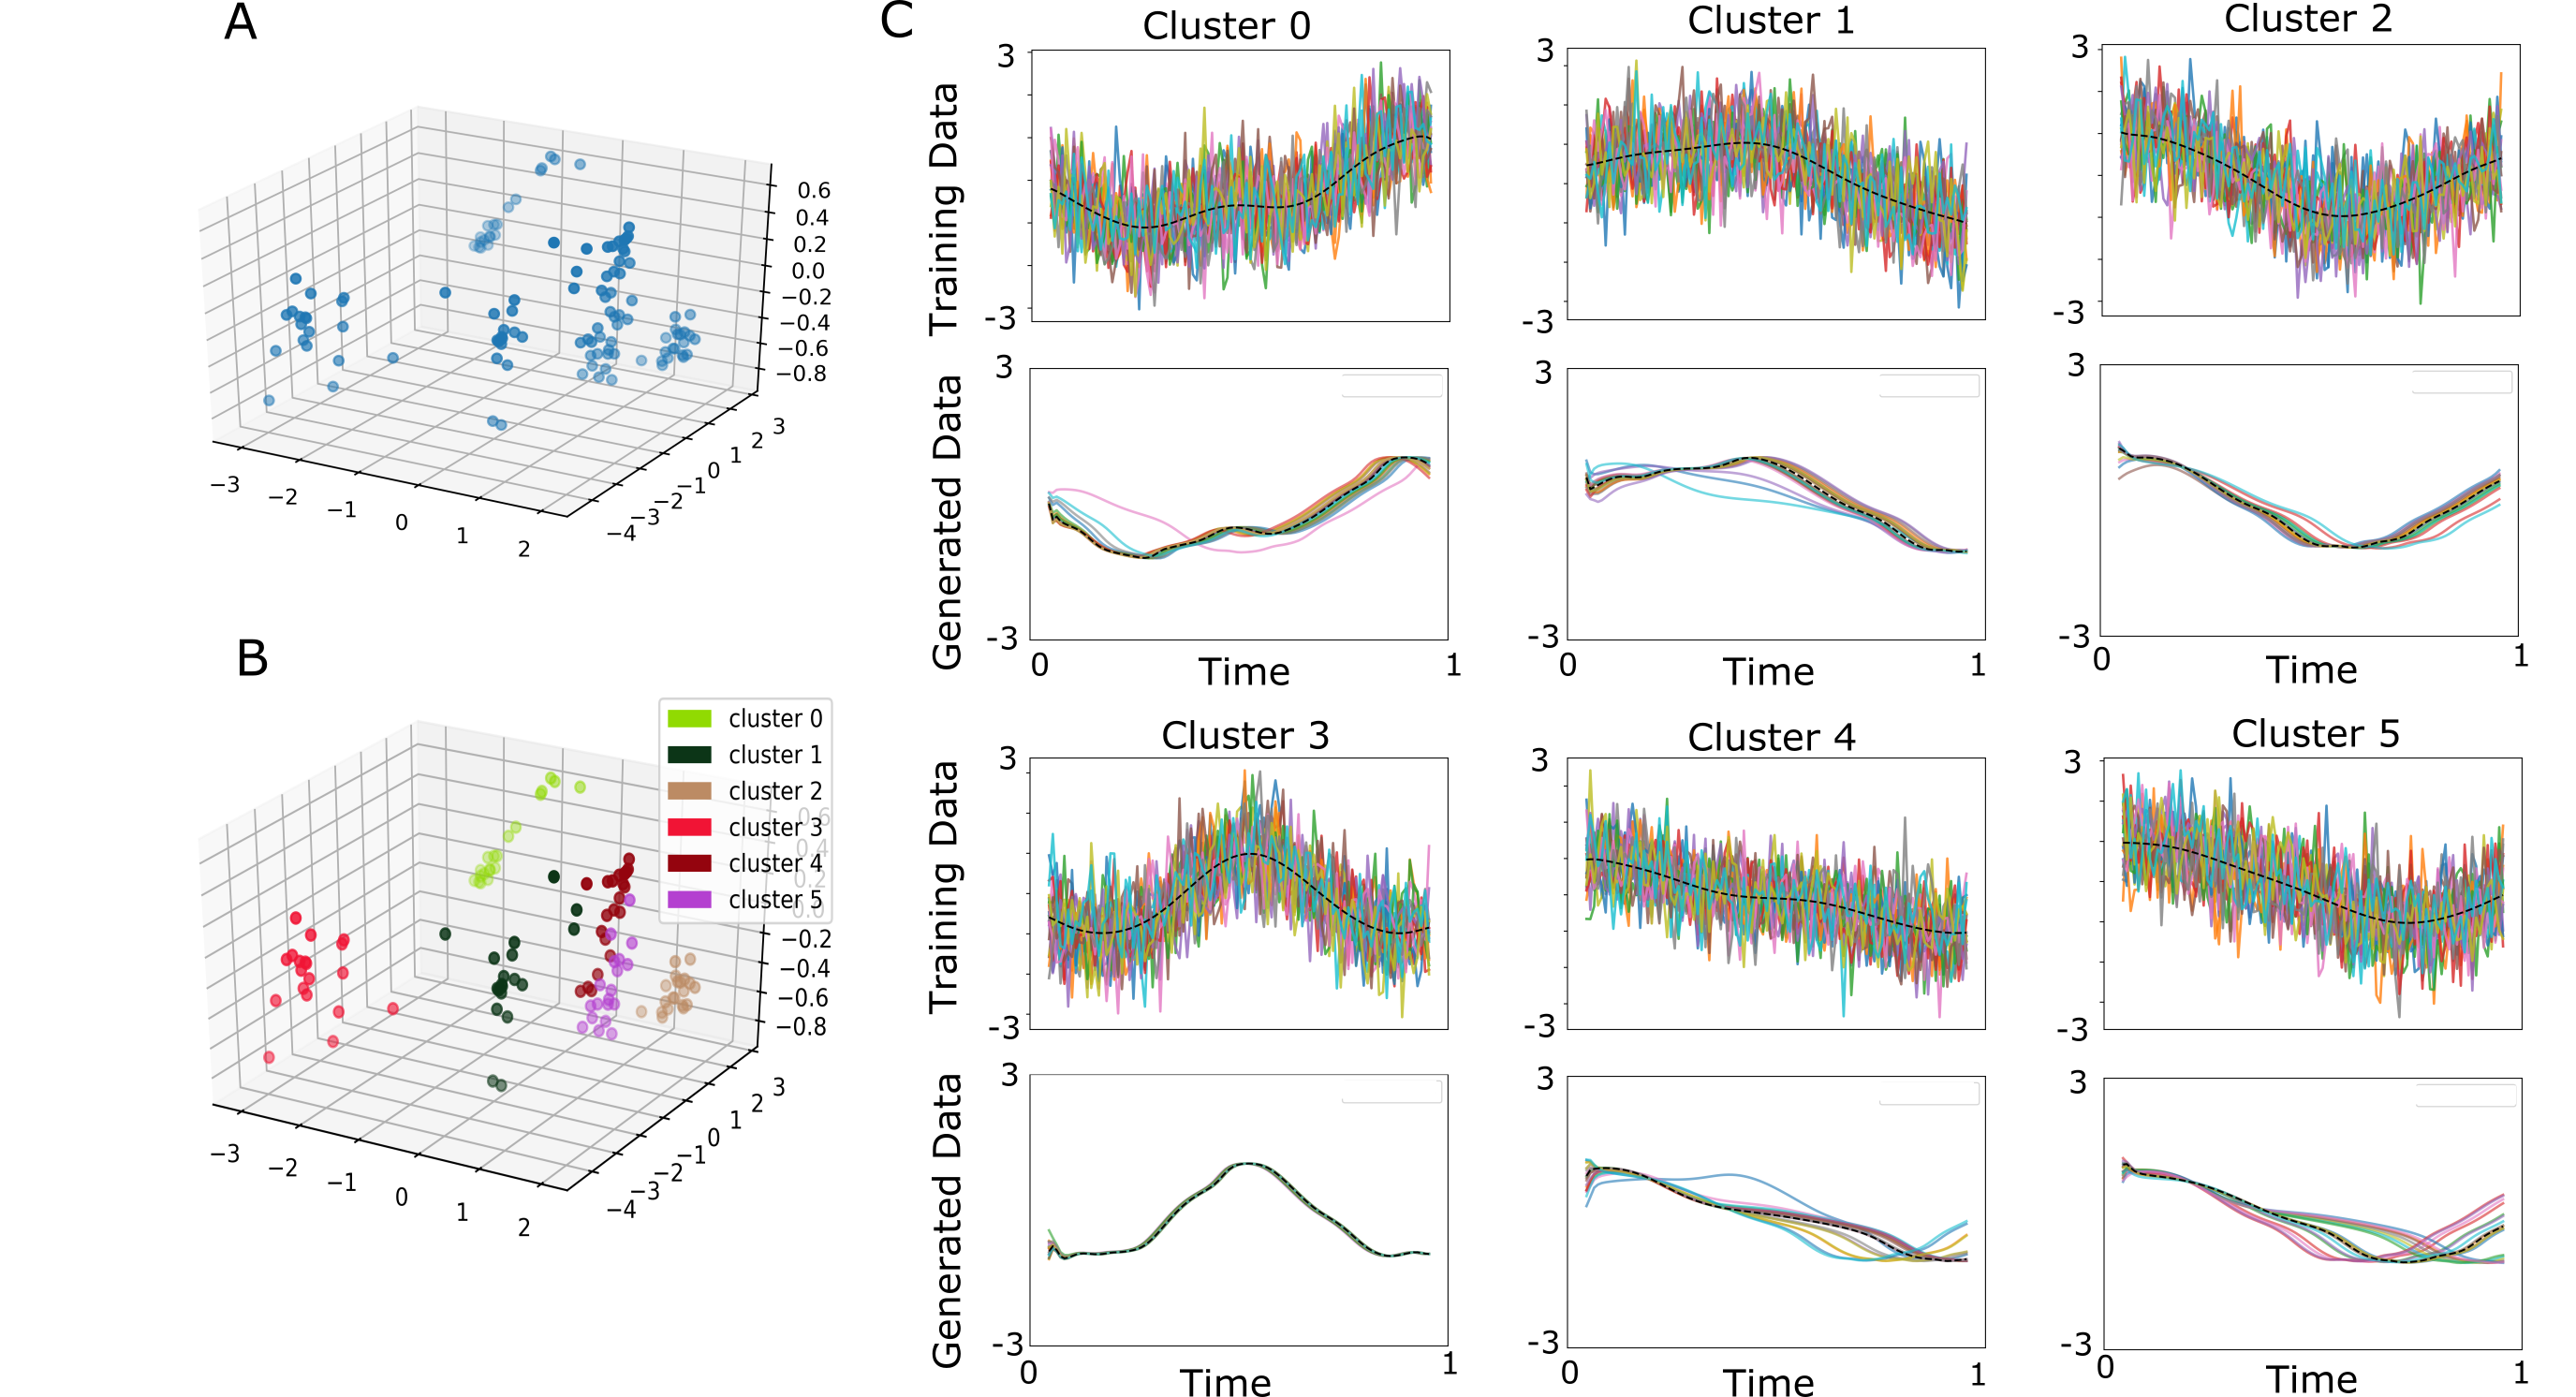
\includegraphics[width=\linewidth]{./figures/noisy_sim.png}
 % archetecture.png: 1149x508 px, 72dpi, 40.53x17.92 cm, bb=0 0 1149 508
    \caption[Demonstration of RVAgene working principle on simulated data with high noise.]{\textbf{Demonstration of RVAgene working principle on simulated data with high noise.} Gaussian noise drawn from $\cN(0,0.7)$ was added to the simulated data to produce a dataset with heavy noise. RVAgene learns the latent space shown in ({\bf A}). ({\bf B}) shows 6 clusters learned by k-means on the learned latent space. ({\bf C}) shows original training data and model generated data from random points in the latent space sampled from $\cN(\mu,0.4\bI)$ around each cluster mean $\mu$ for each of the 6 clusters detected by k-means.}
  \label{fig:figS1}
\end{figure}
\end{center}
\newpage

\begin{center}
\begin{figure}[H]
  \includegraphics[width=\linewidth]{./figures/sl_ESC_r.png}
 % archetecture.png: 1149x508 px, 72dpi, 40.53x17.92 cm, bb=0 0 1149 508
    \caption[Characterization of gene dynamics by linear fit using Pearson correlation coefficient for 5 sample genes in the ESC differentiation dataset]{Characterization of gene dynamics by linear fit using Pearson correlation coefficient for 5 sample genes in the ESC differentiation dataset  \citep{Klein2015}. Blue lines represents original data and orange lines represents linear fits. The Pearson correlation coefficient $r$ is given for each plot.}
  \label{fig:figS2}
\end{figure}
\end{center}
\newpage

\begin{center}
\centering
\begin{figure}[H]
  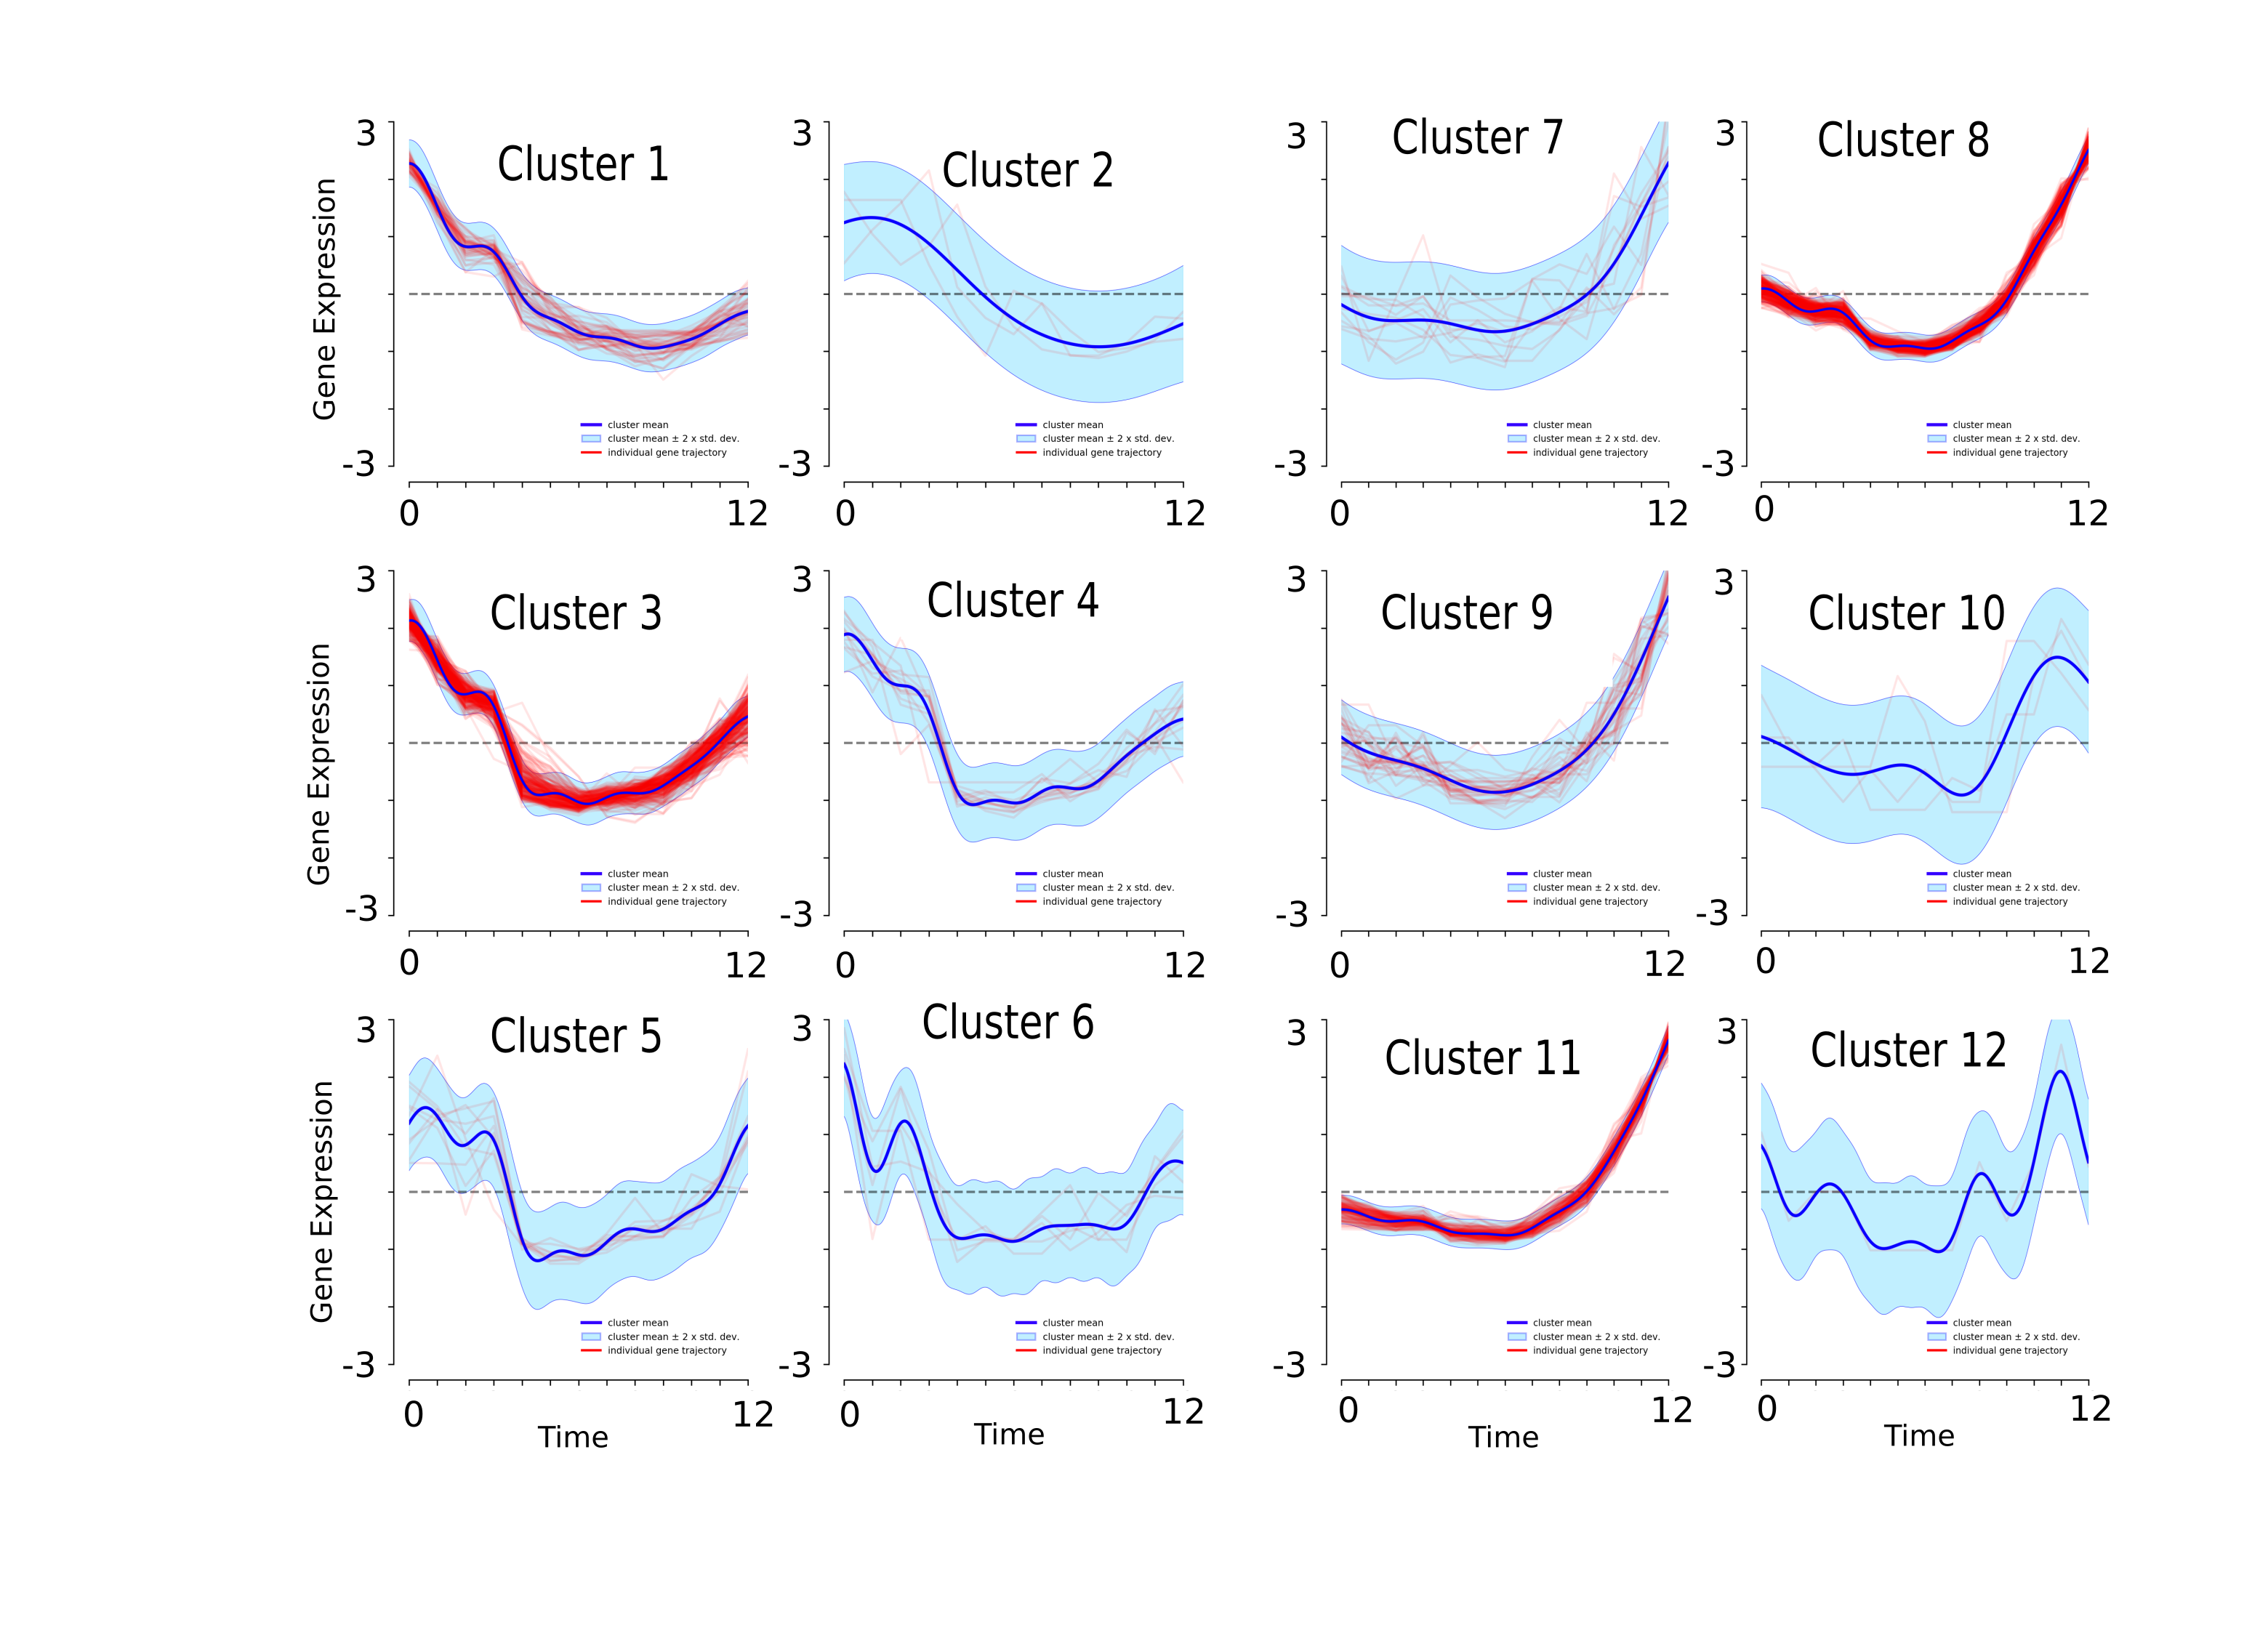
\includegraphics[width=\linewidth,height=0.4\textheight]{figures/fig4.png}
 % archetecture.png: 1149x508 px, 72dpi, 40.53x17.92 cm, bb=0 0 1149 508
    \caption[Clusters detected by the unsupervised clustering algorithm DPGP for ESC differentiation.]{\textbf{Clusters detected by the unsupervised clustering algorithm DPGP for ESC differentiation.} Clusters detected by DPGP in the ESC differentiation dataset  \citep{Klein2015} with default hyperparameters showing cluster means (black), mean $\pm$ 2 s.d. in (blue) and cluster members (red). }
   \label{fig:figS3}
\end{figure}
\end{center}
\newpage
\begin{center}
\begin{figure}
  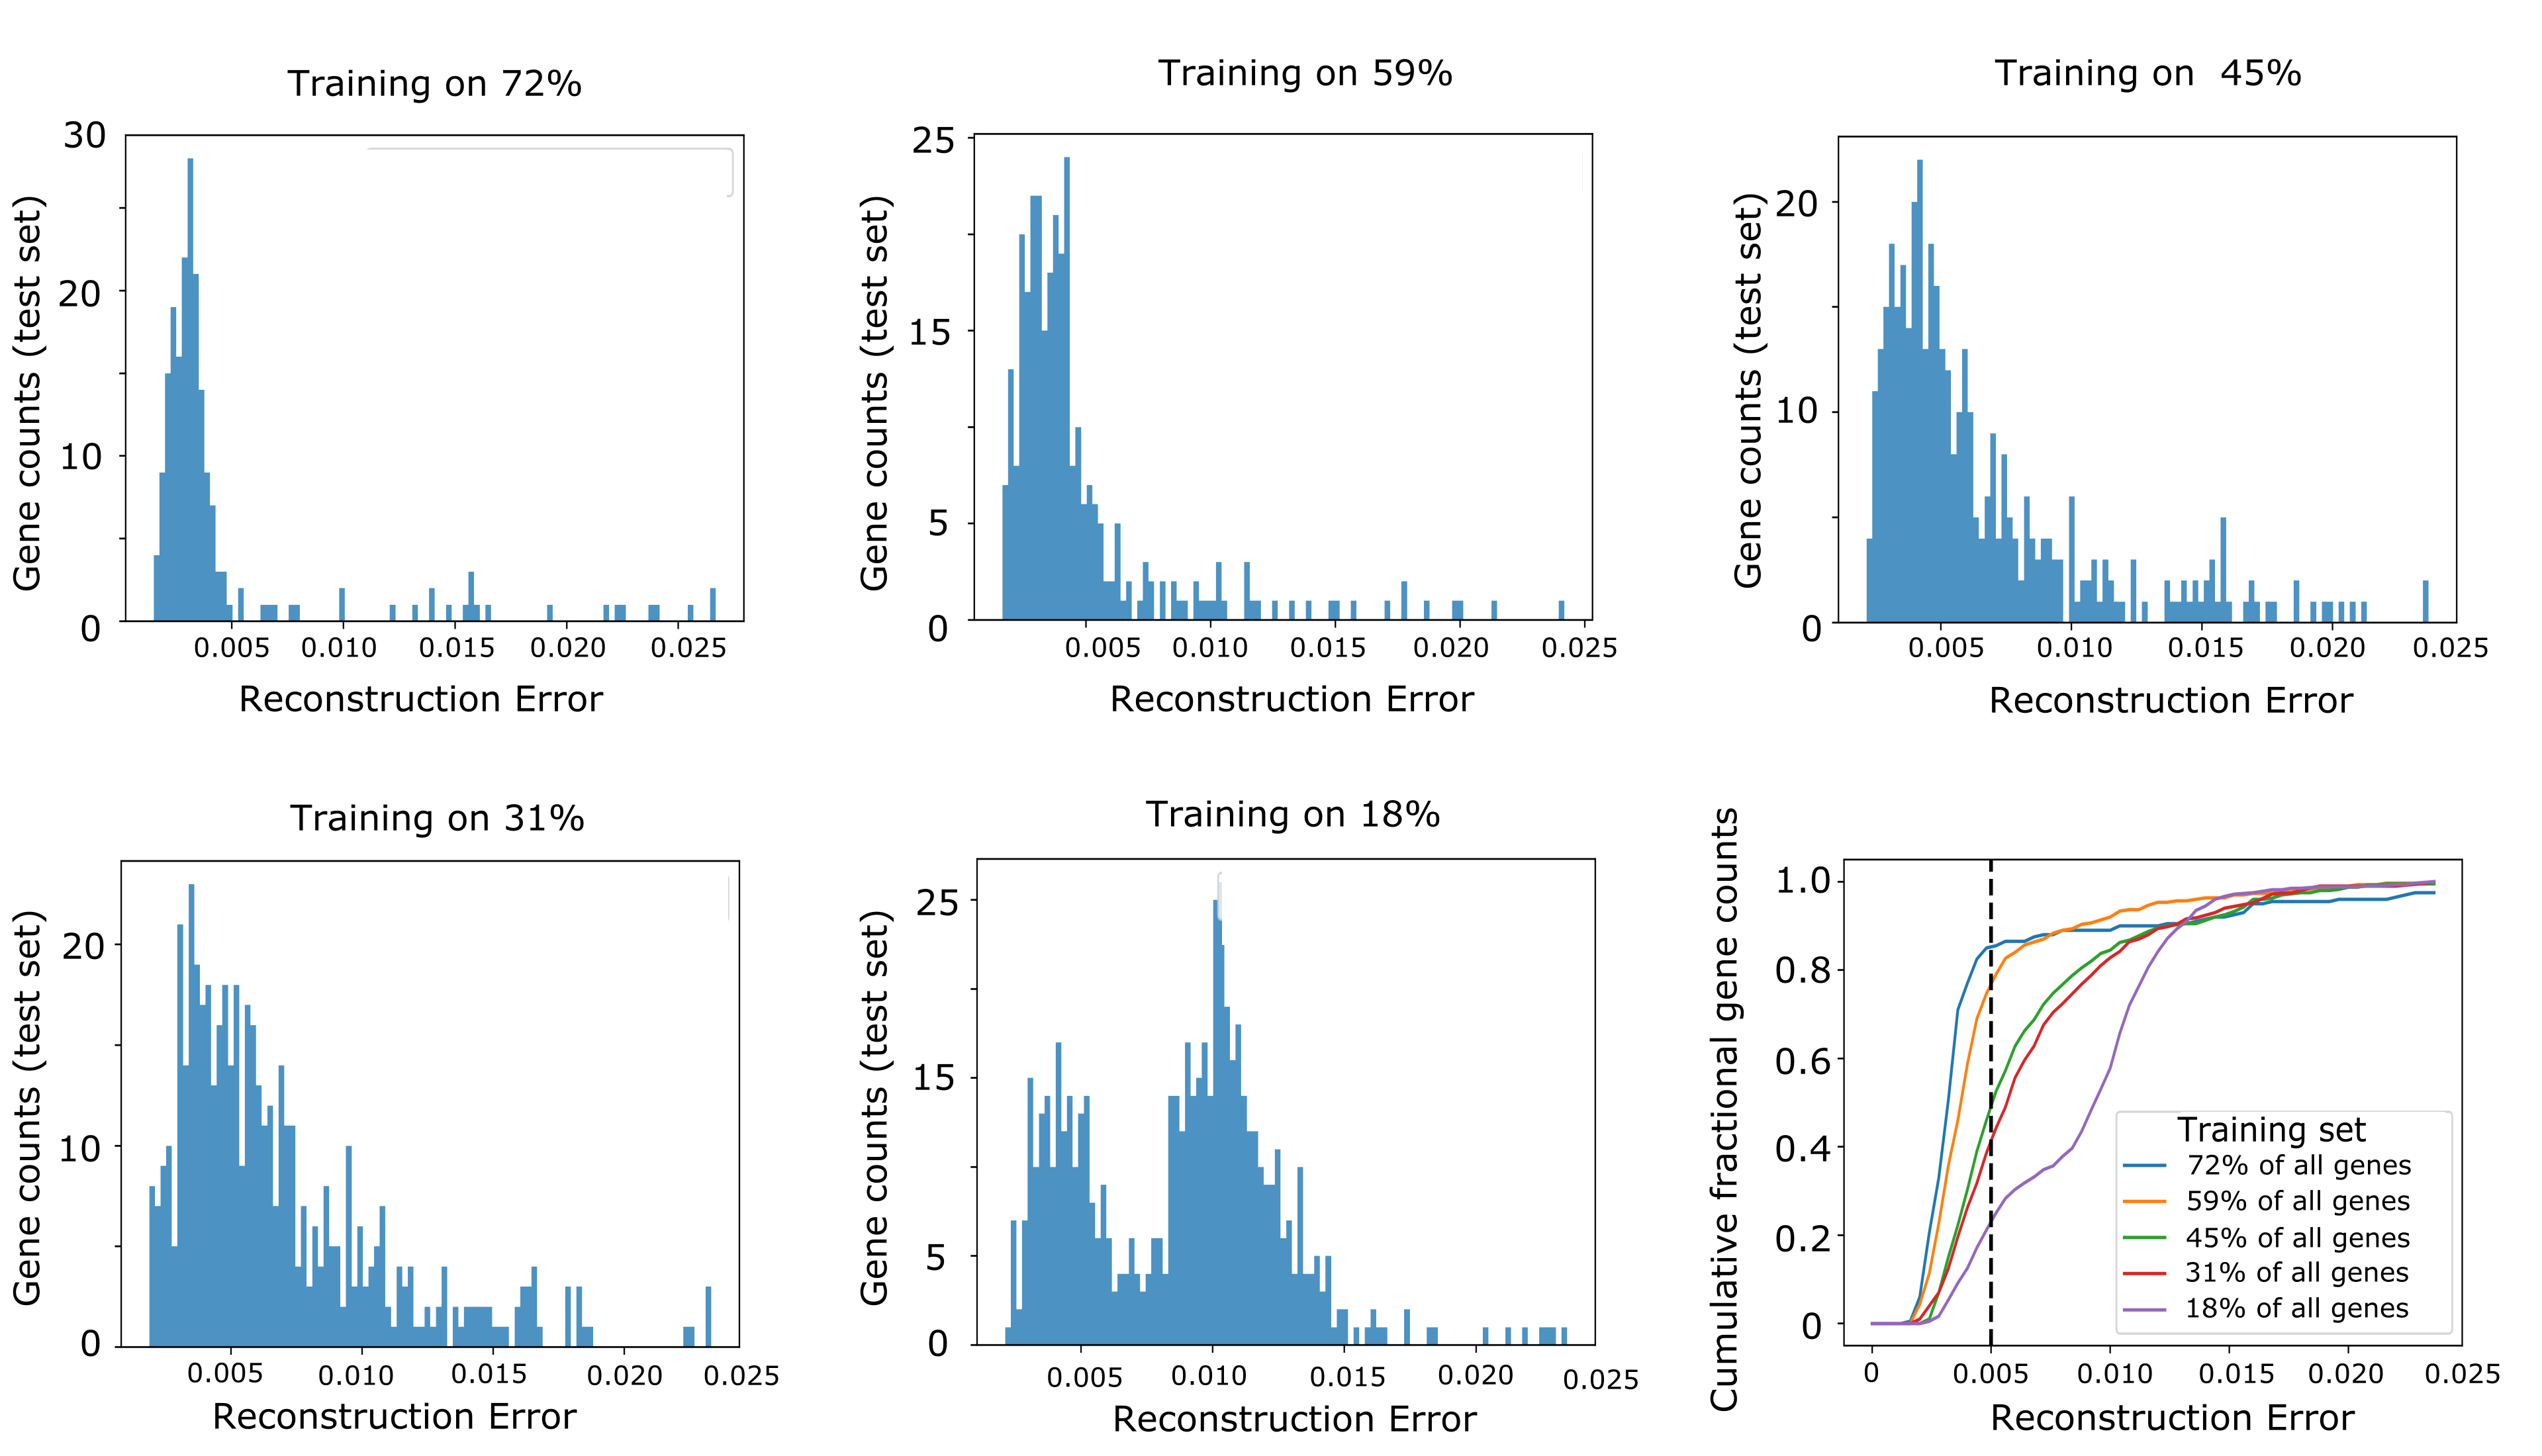
\includegraphics[width=\linewidth]{./figures/supp_varying_test_set_sizes.png}
 % archetecture.png: 1149x508 px, 72dpi, 40.53x17.92 cm, bb=0 0 1149 508
    \caption[Accuracy of RVAgene reconstructions for different train/test group sizes.]{{\bf Accuracy of RVAgene reconstructions for different train/test group sizes.} Distributions of reconstruction errors on randomly sampled sets of test genes, where the full data were split into test groups of: 200 genes (train on 72\%), 300 genes (train on 59\%), 400 genes (train on 45\%), 500 genes (train on 31\%), and 600 genes (train on 18\%). Cumulative fractional distribution of reconstruction errors (cumulative count/test set size) for all groups.}
  \label{fig:figS4}
\end{figure}
\end{center}
\newpage

\begin{center}
\begin{figure}[H]
  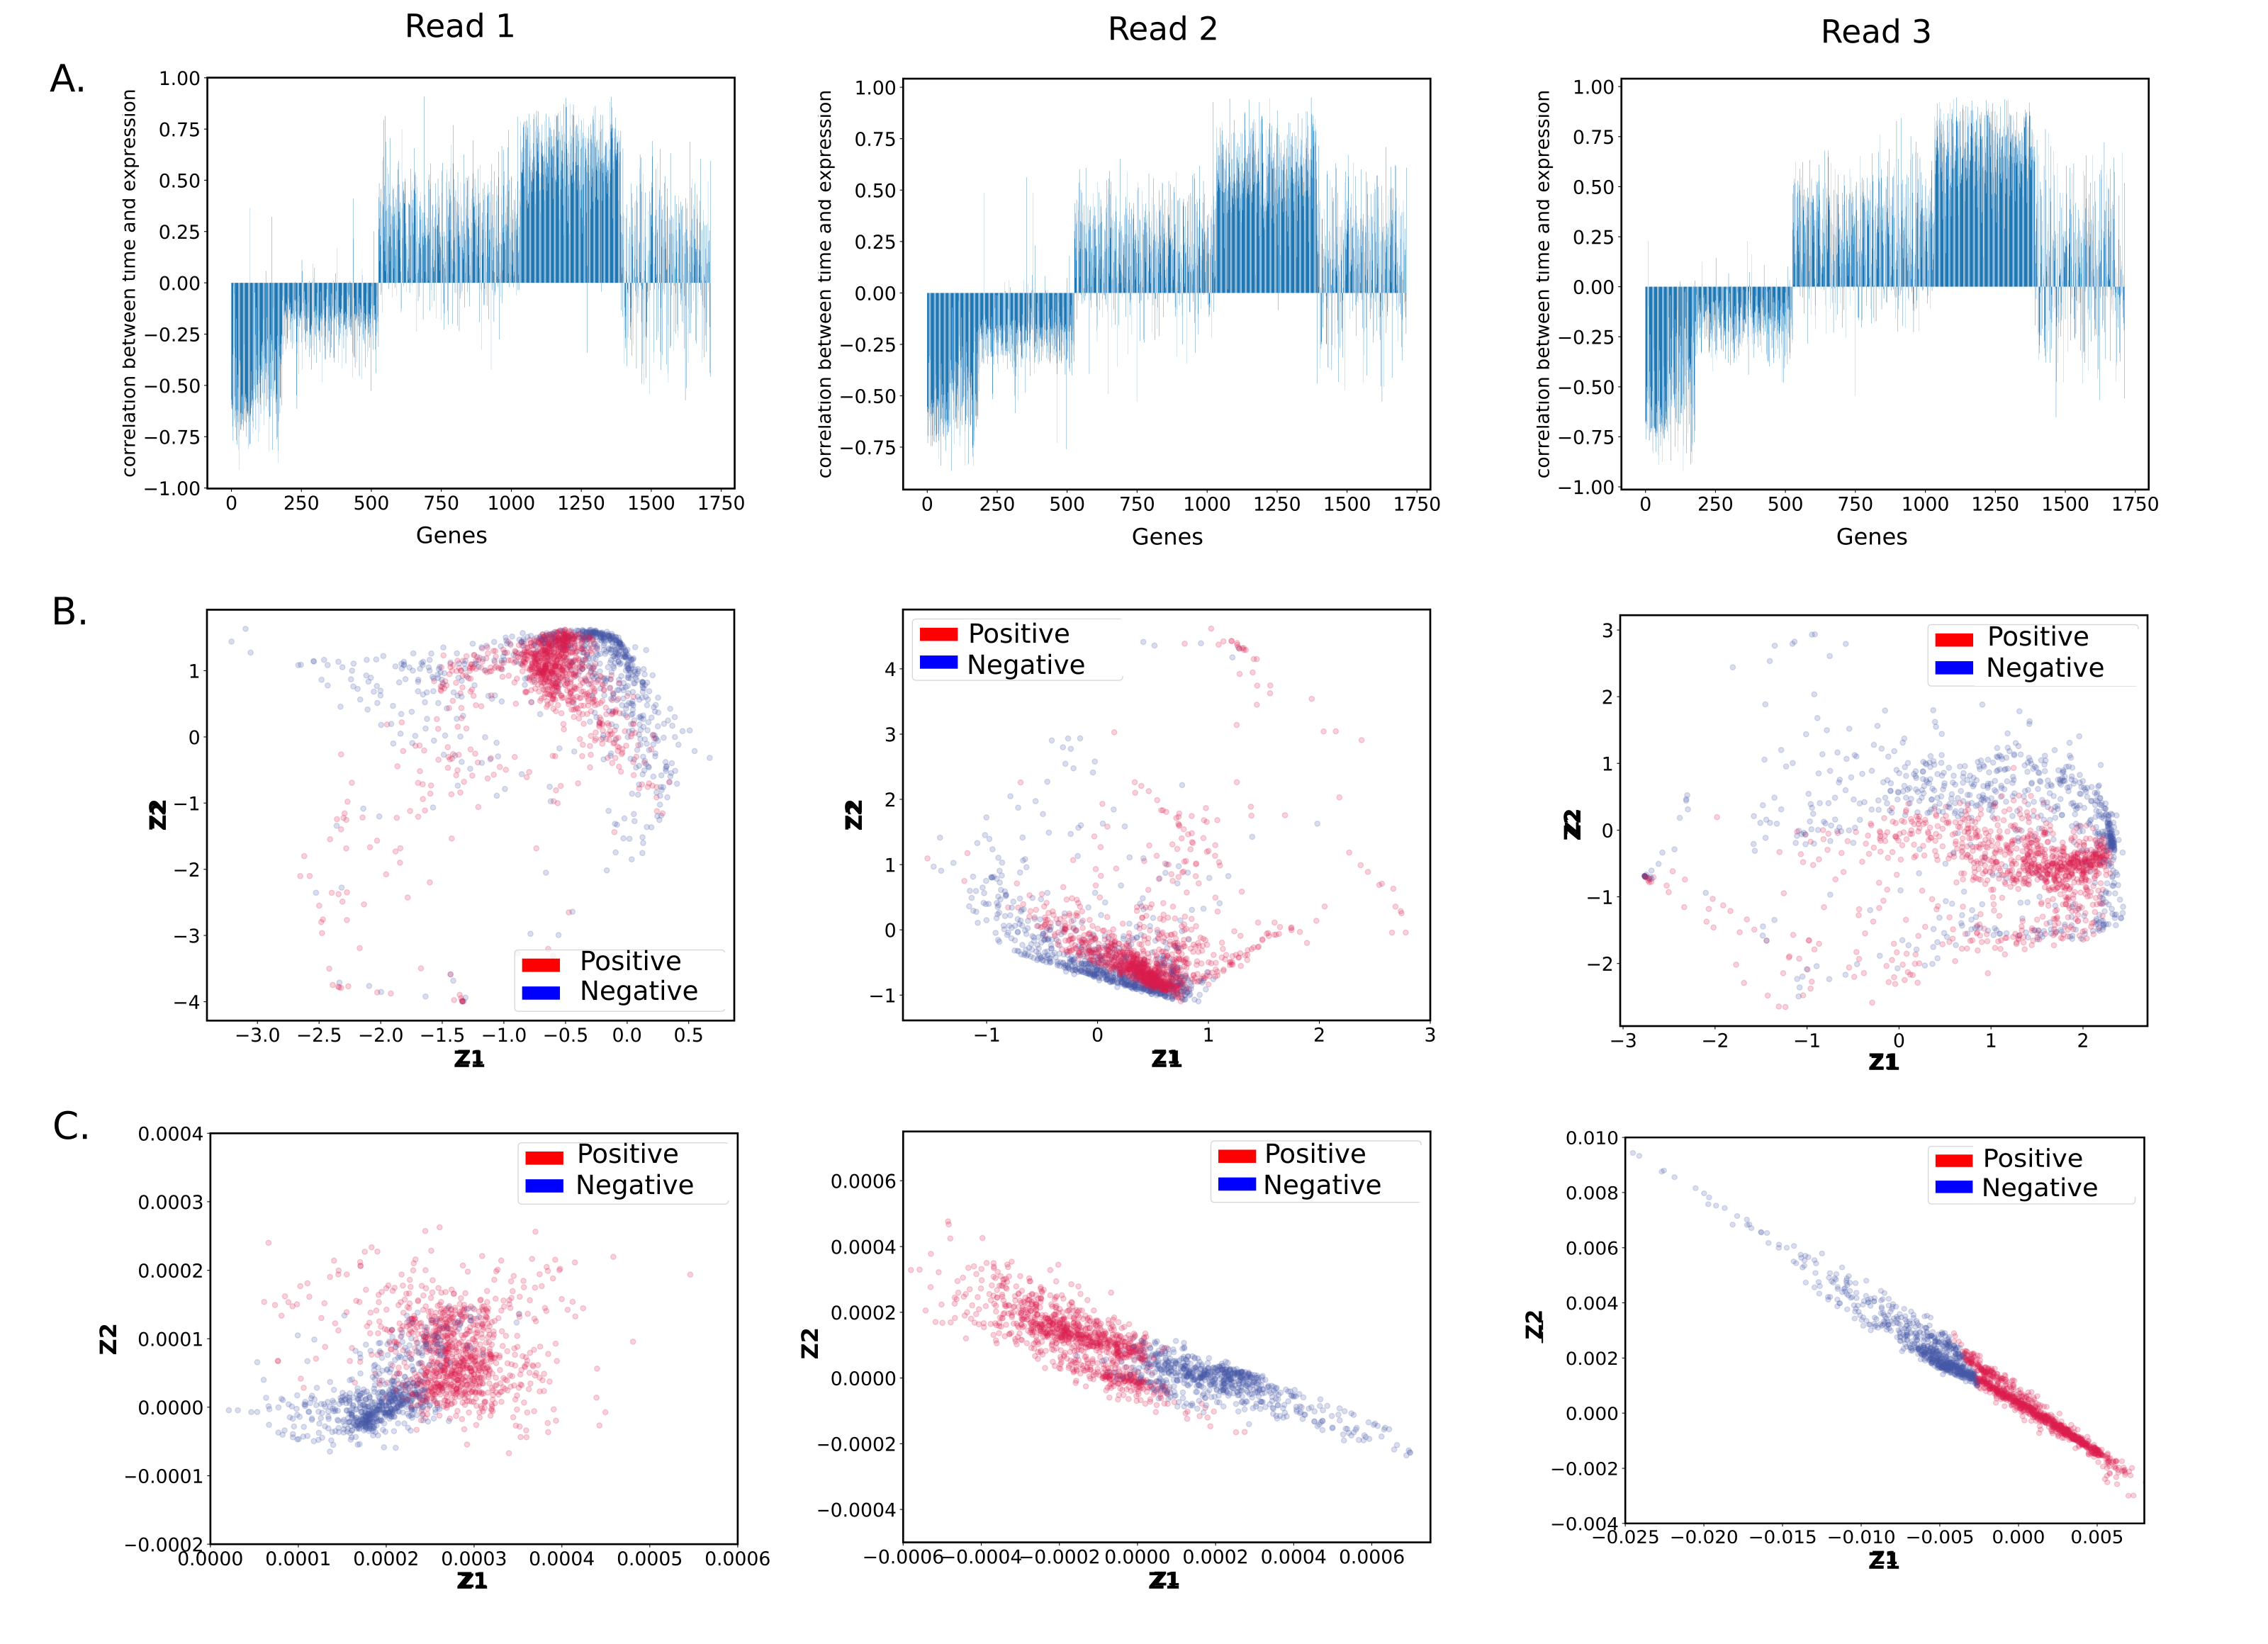
\includegraphics[width = \linewidth]{figures/fig8.png}
 % archetecture.png: 1149x508 px, 72dpi, 40.53x17.92 cm, bb=0 0 1149 508
    \caption[Modeling response to kidney injury and analysis of linear fits.]{\textbf{Modeling response to kidney injury and analysis of linear fits.}
    ({\bf A}) Pearson correlation coefficients between gene expression and time for each differentially expressed gene in the kidney injury dataset for each of the 3 replicates \citep{liu2017molecular}. ({\bf B}) RVAgene latent space representation of fitted model for each replicate; color represents positive or negative correlation coefficients. ({\bf C}) RVAgene latent space representation learnt for the same three replicates as in (B), but where every input gene was normalized  so that its expression sums to 1.}
  \label{fig:figS5}
\end{figure}
\end{center}
\newpage

\begin{center}
\begin{figure}[H]
  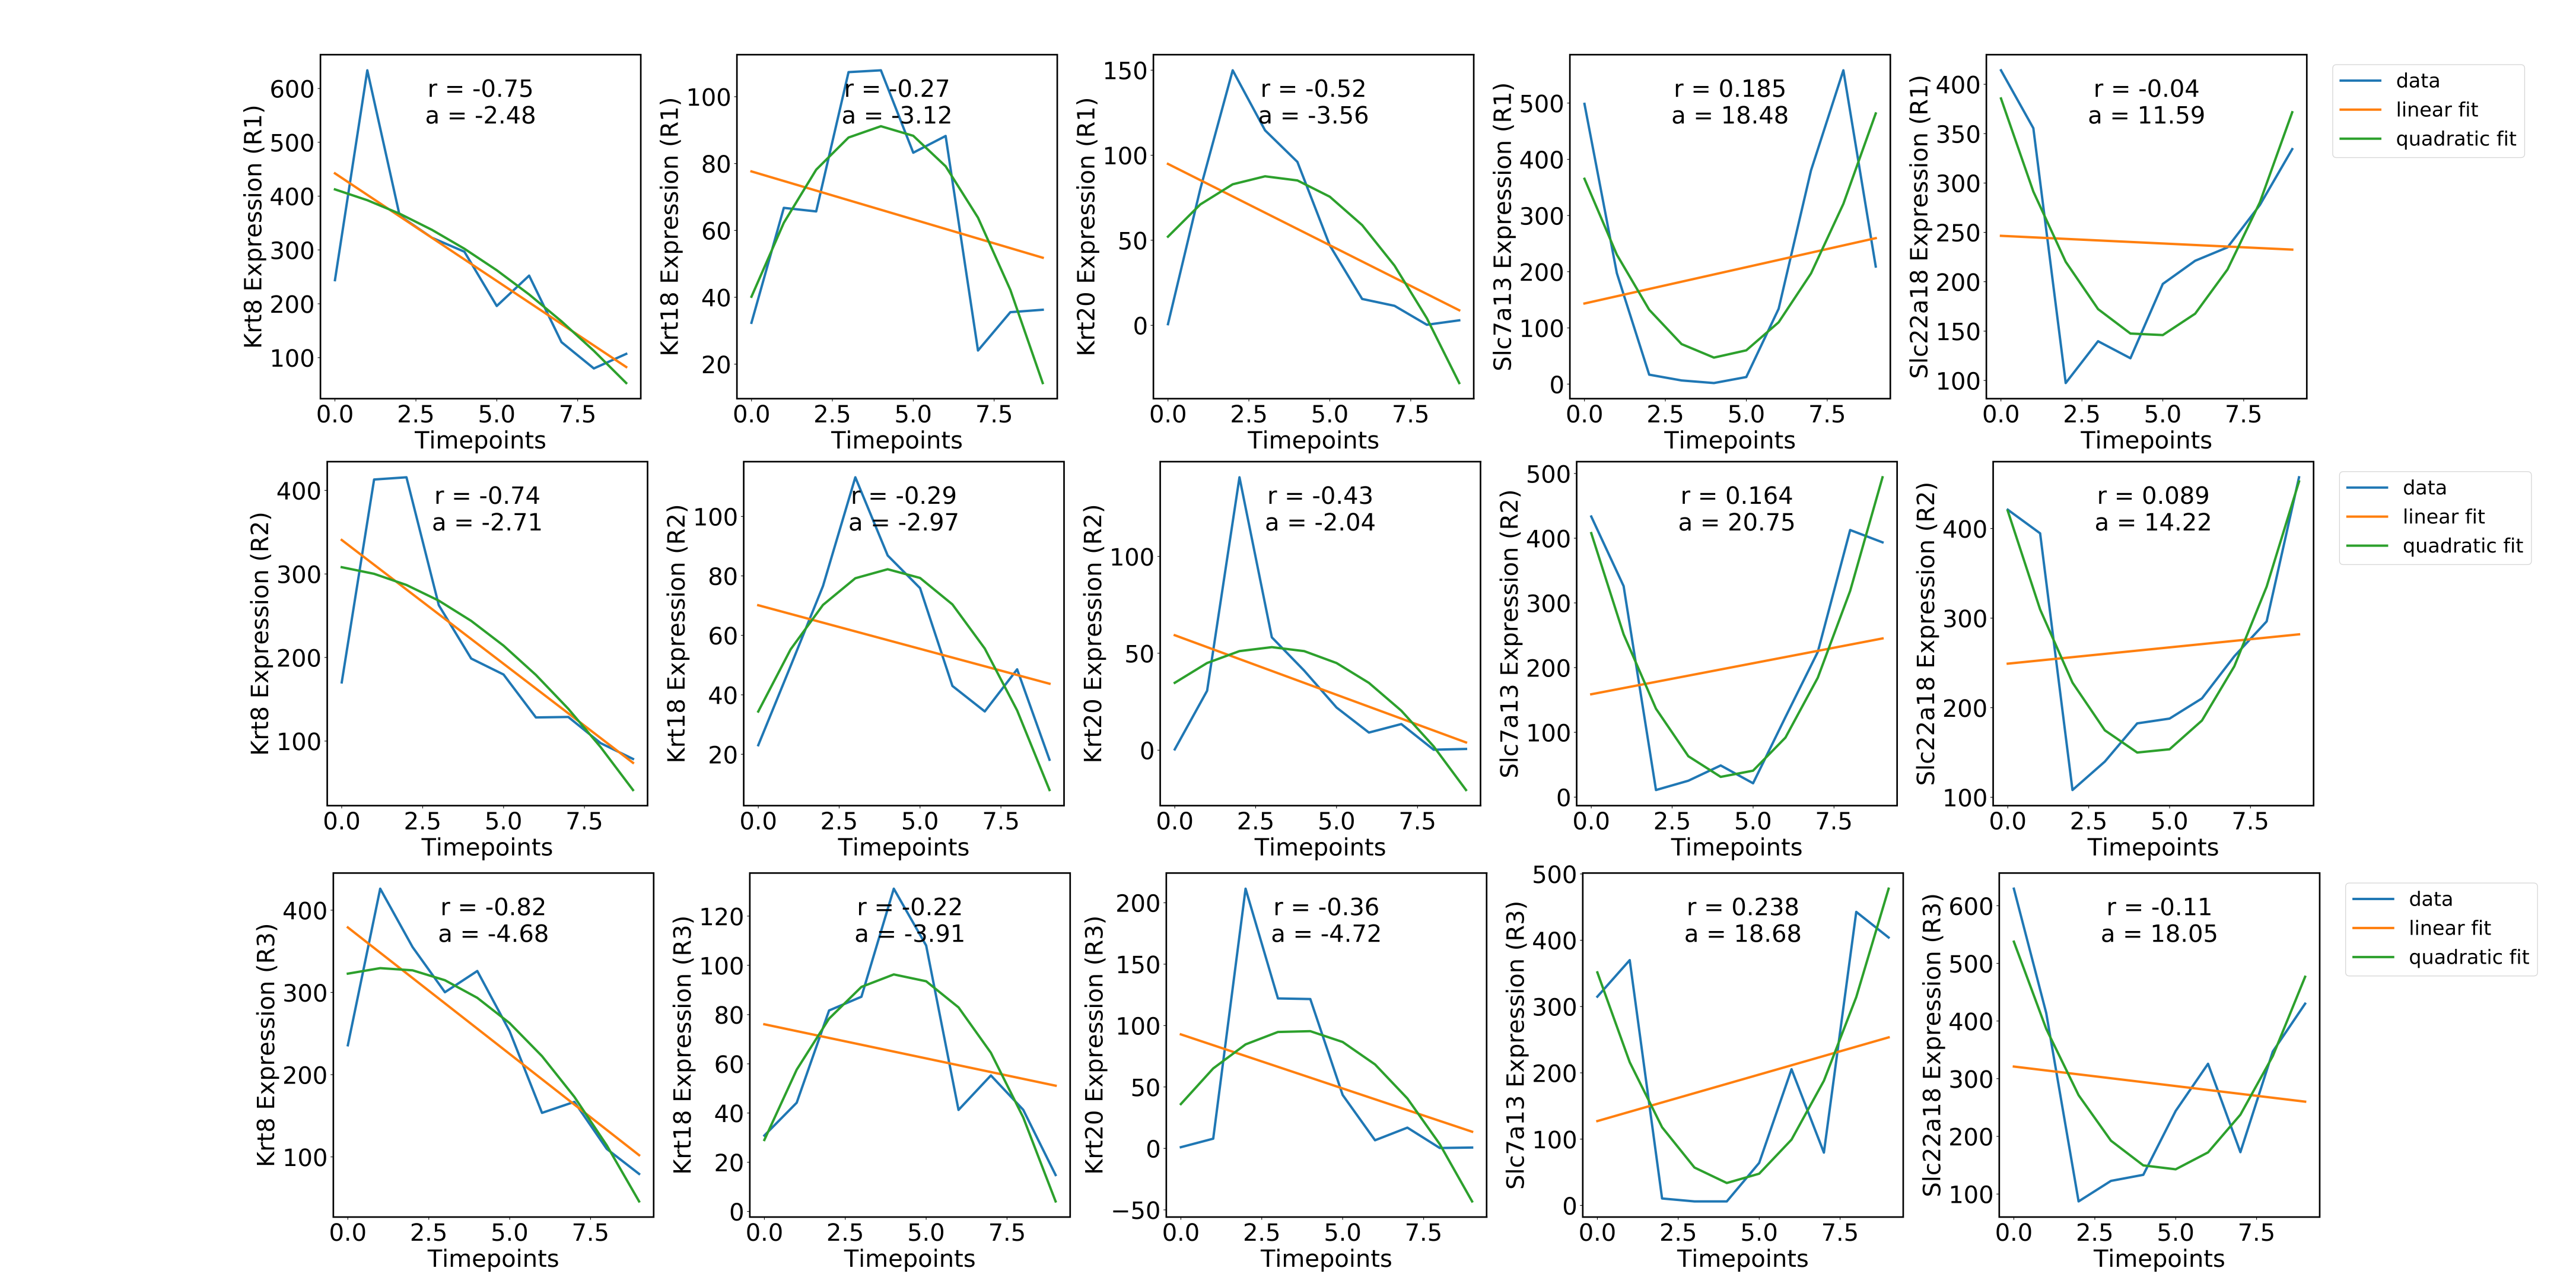
\includegraphics[width=\linewidth]{./figures/sl_JCI_r.png}
 % archetecture.png: 1149x508 px, 72dpi, 40.53x17.92 cm, bb=0 0 1149 508
    \caption[Comparison of linear and quadratic fits to describe gene dynamics in response to kidney injury.]{\textbf{Comparison of linear and quadratic fits to describe gene dynamics in response to kidney injury.}
    For each of the three replicates (R1-R3), five genes are shown, with experimental data (blue), linear fit (orange), and quadratic fit (green). 
    Pearson correlation coefficients, $r$, and quadratic coefficients, $a$ ($x = at^2 + bt + c$), are given for each plot.}
  \label{fig:figS6}
\end{figure}
\end{center}
\newpage

\begin{center}
\begin{figure}[H]
  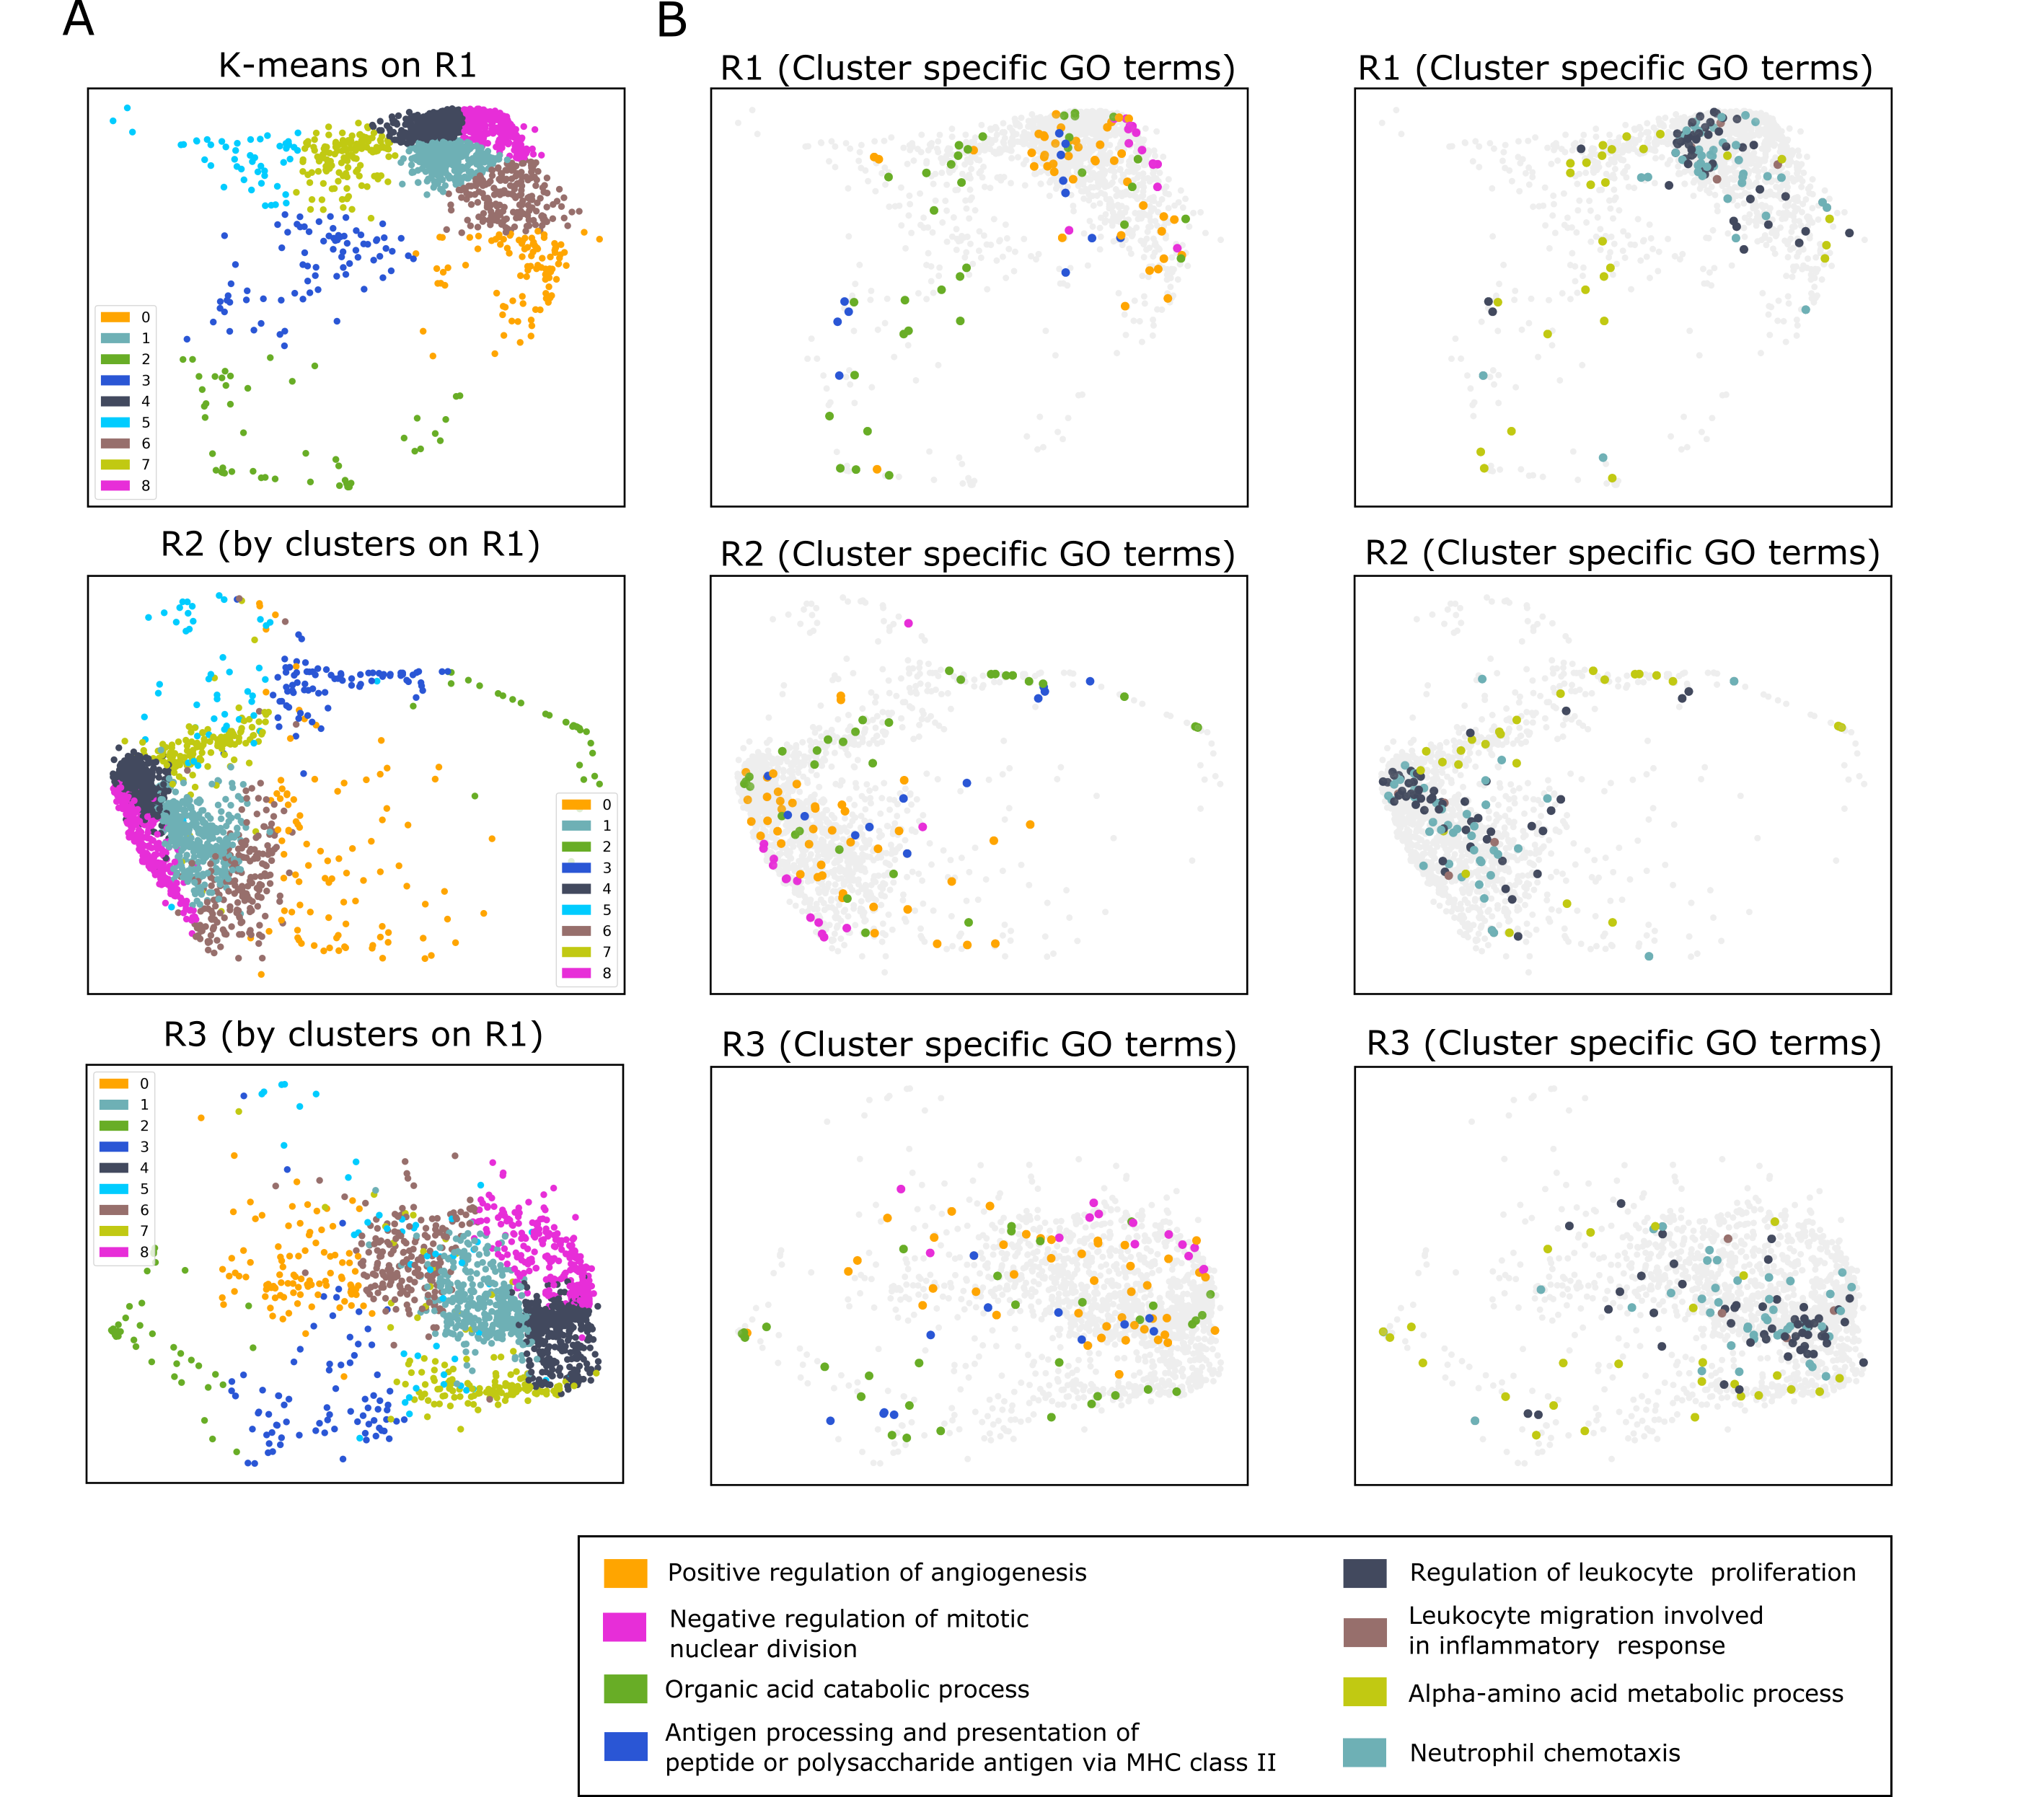
\includegraphics[width=\linewidth]{./figures/supp_go.png}
 % archetecture.png: 1149x508 px, 72dpi, 40.53x17.92 cm, bb=0 0 1149 508
    \caption[Clustering on R1 and cluster specific GO enrichment analysis.]{\textbf{Clustering on R1 and cluster specific GO enrichment analysis.} We performed k-means clustering on latent space learned by RVAgene on R1 with $k=9$. We also show learned latent space on R2 and R3 annotated by the clustering done on R1. All clusters (except cluster 5) appears well preserved. We perform GO analysis for each cluster and select one significant GO term from each cluster (except cluster 5) and show how all genes in the dataset corresponding to each GO term appears on the latent space for all three replicates. }
  \label{fig:figS8}
\end{figure}
\end{center}
\newpage

\begin{center}
\begin{figure}[H]
  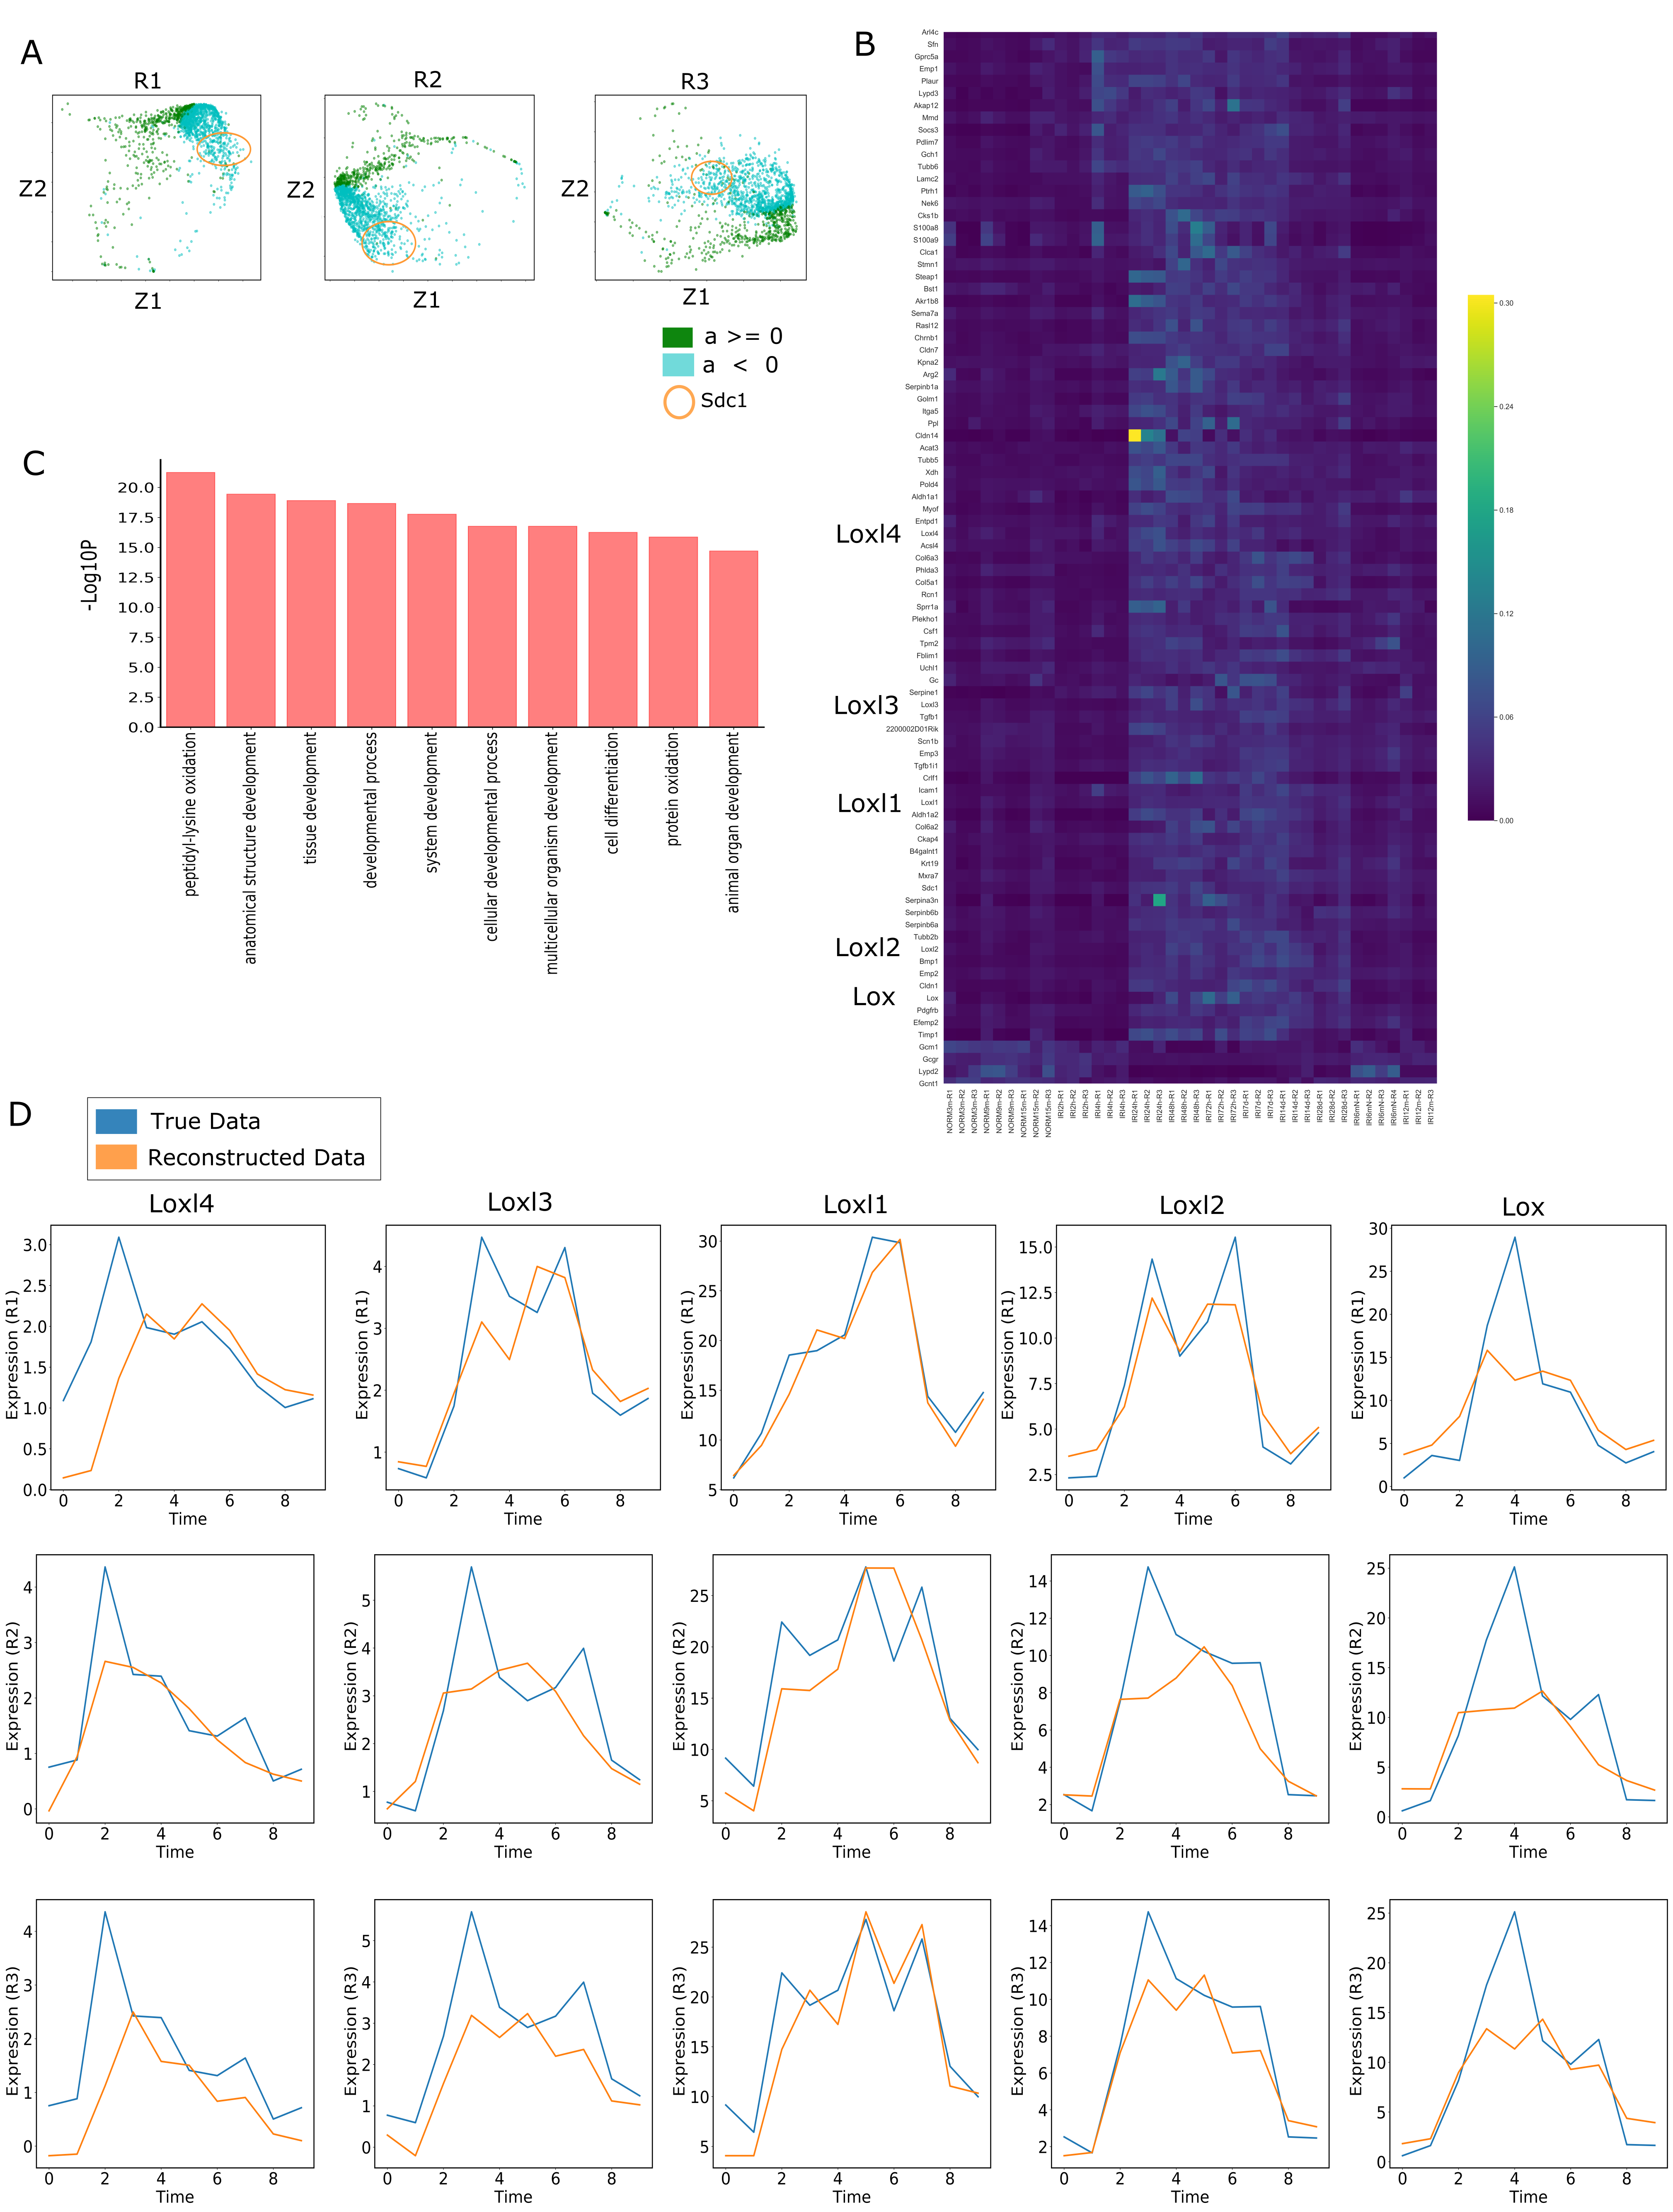
\includegraphics[width=\linewidth]{./figures/sdc_sl.png}
 % archetecture.png: 1149x508 px, 72dpi, 40.53x17.92 cm, bb=0 0 1149 508
    \caption[RVAgene latent space captures biological processes driving concordant gene expression changes (Sdc1).]{{\bf (A)} Latent space representations for replicates R1-R3 with local neighborhoods of Sdc1 marked (circles). ({\bf B}) Heatmap of expression changes over time course of injury for the Sdc1 neighborhood genes in the intersection of R1-R3; selected genes highlighted.  ({\bf C}) Histogram of -log10 p values of top GO terms for biological processes for gene set in (B).
    {\bf D}) Reconstructed vs true data plotted for each of the Lox genes identified in (B).}
  \label{fig:figS7}
\end{figure}
\end{center}

\begin{center}
\begin{figure}[H]
  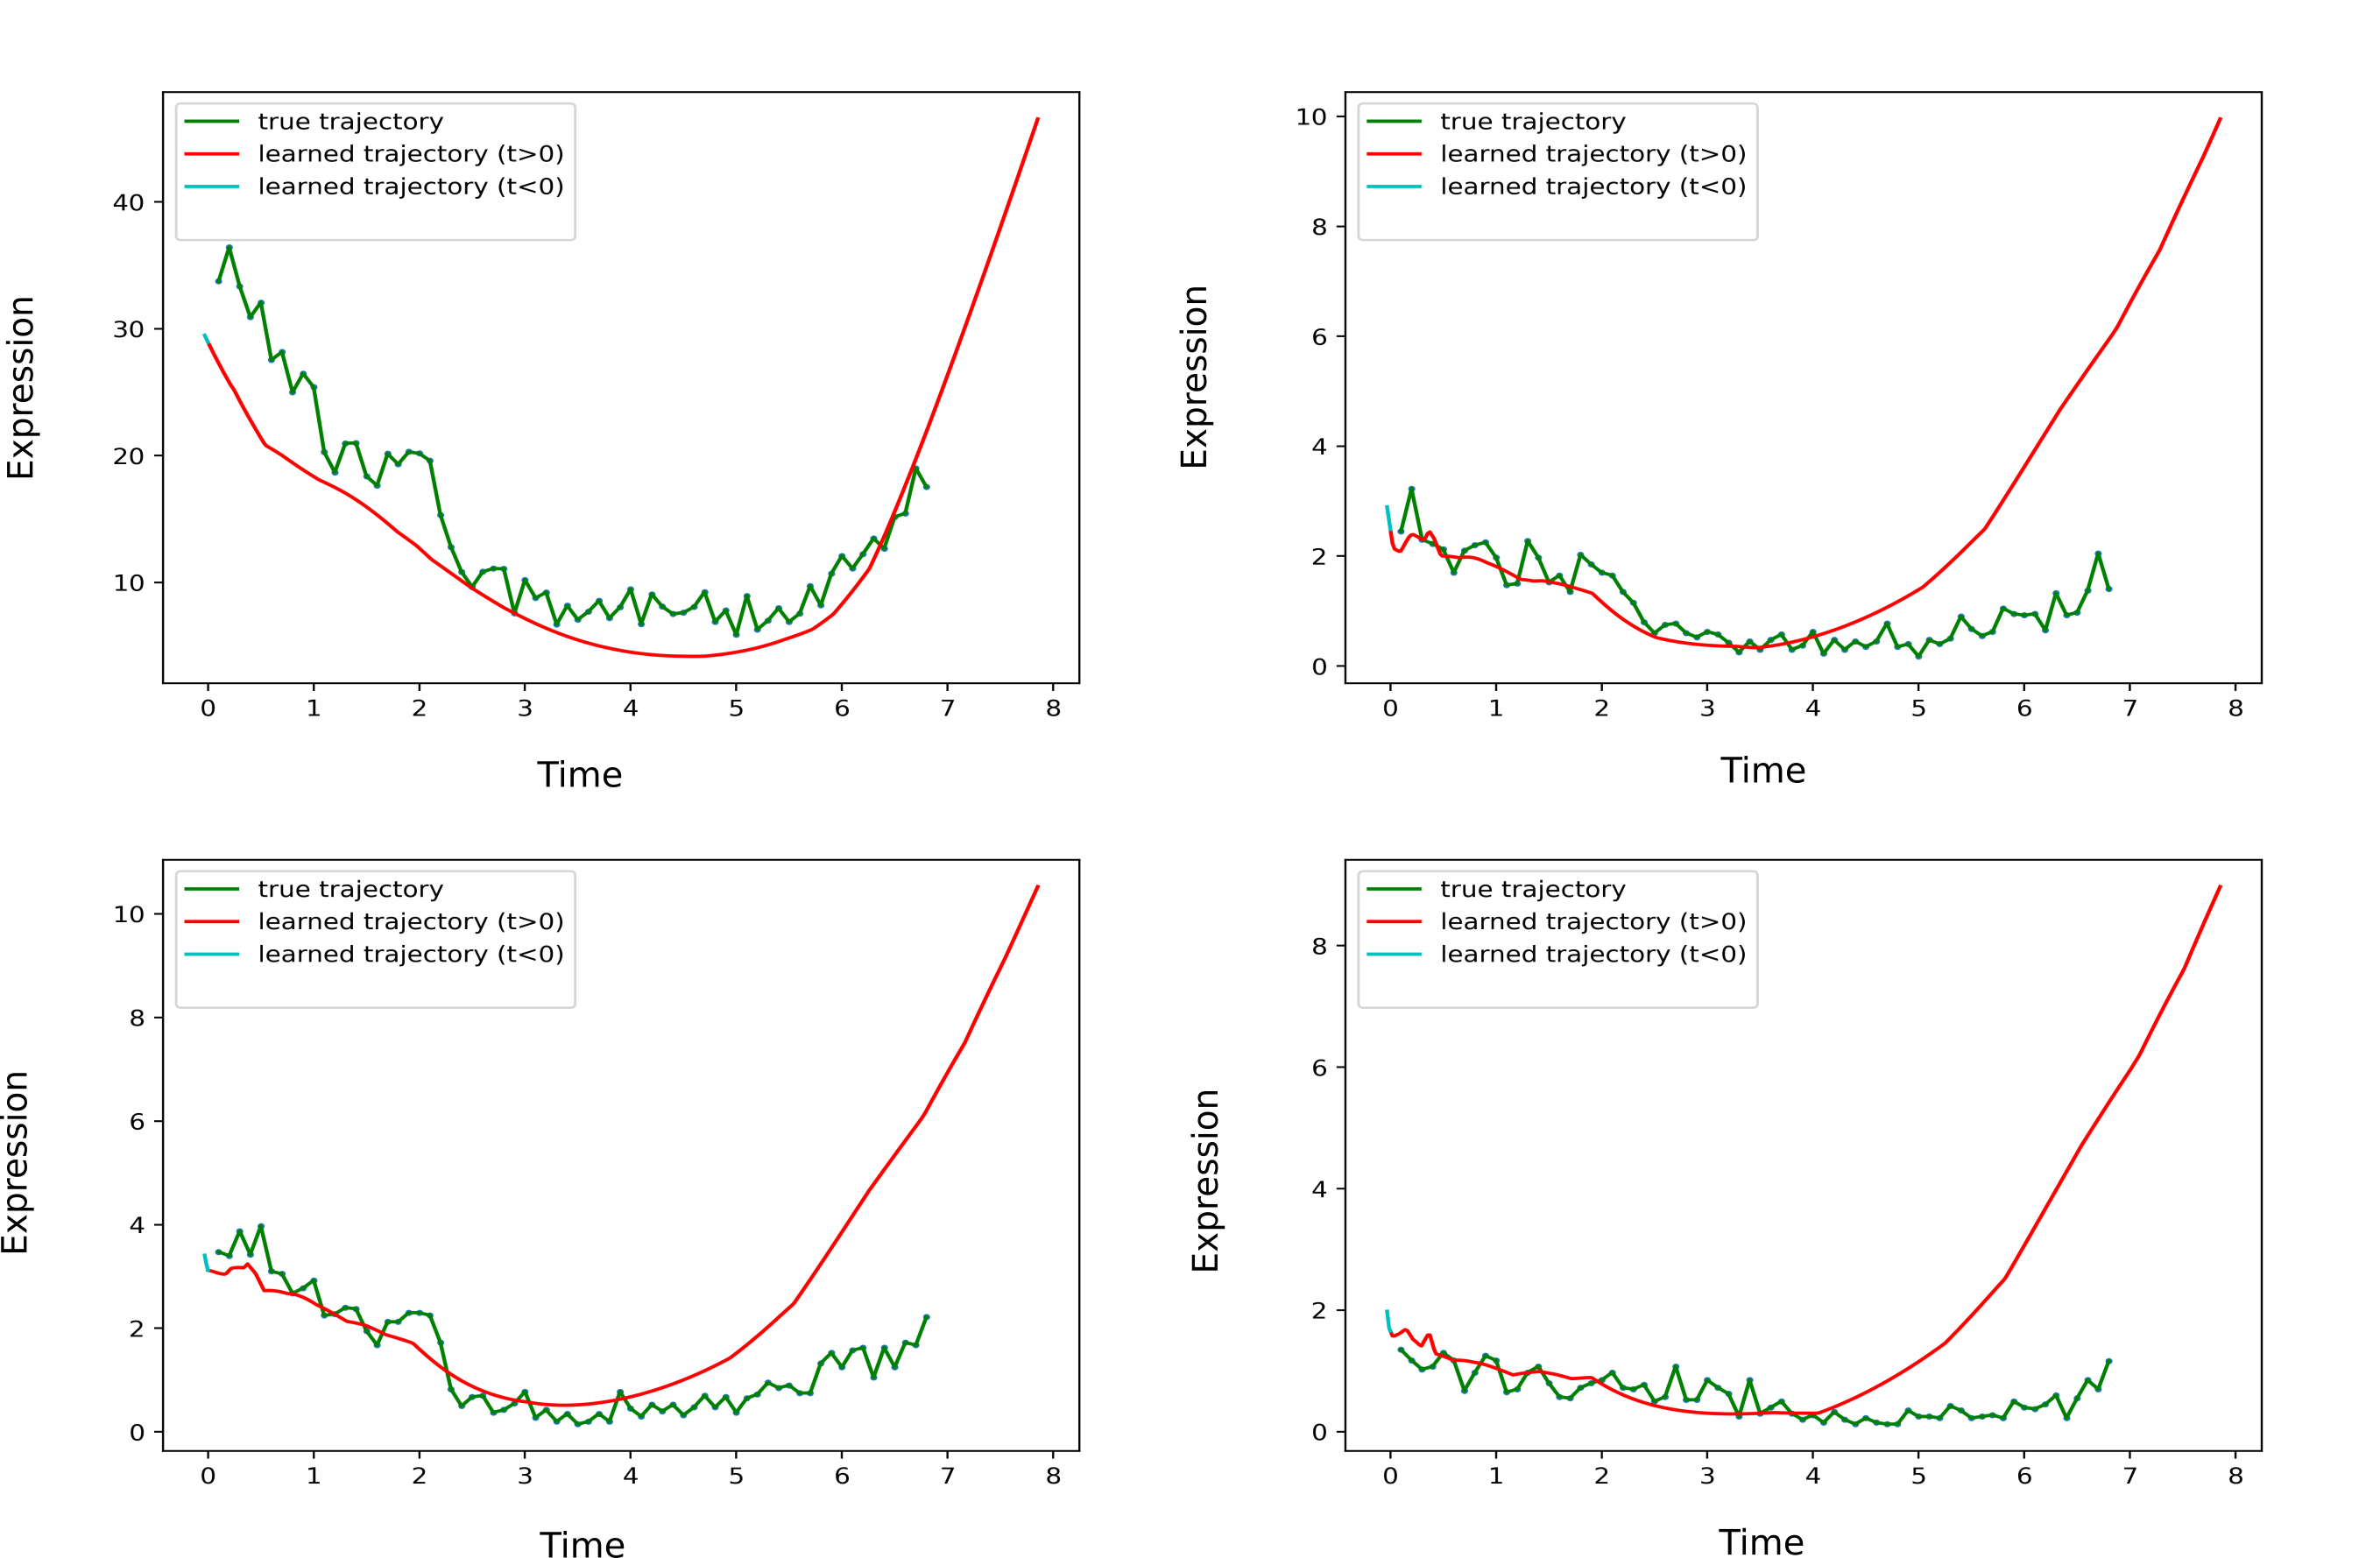
\includegraphics[width=\linewidth]{./figures/latent_ode_val_underfit.png}
 % archetecture.png: 1149x508 px, 72dpi, 40.53x17.92 cm, bb=0 0 1149 508
    \caption[Examples of continuous time prediction of ESC differentiation.]{\textbf{Examples of continuous time prediction of ESC differentiation.} Reconstruction (up to $t=6.8$) and future prediction (for $t>6.8$) for 4 example genes by a  latent ODE \citep{chen2018neural} trained on ESC data \citep{Klein2015} for 1000000 iterations, showing a good fit for the initial timepoints, but underfitting for the later timepoints.}
  \label{fig:figS9}
\end{figure}
\end{center}

%% RNASCAPE SUPP FIGURES
\begin{center}
\begin{figure}[H]
  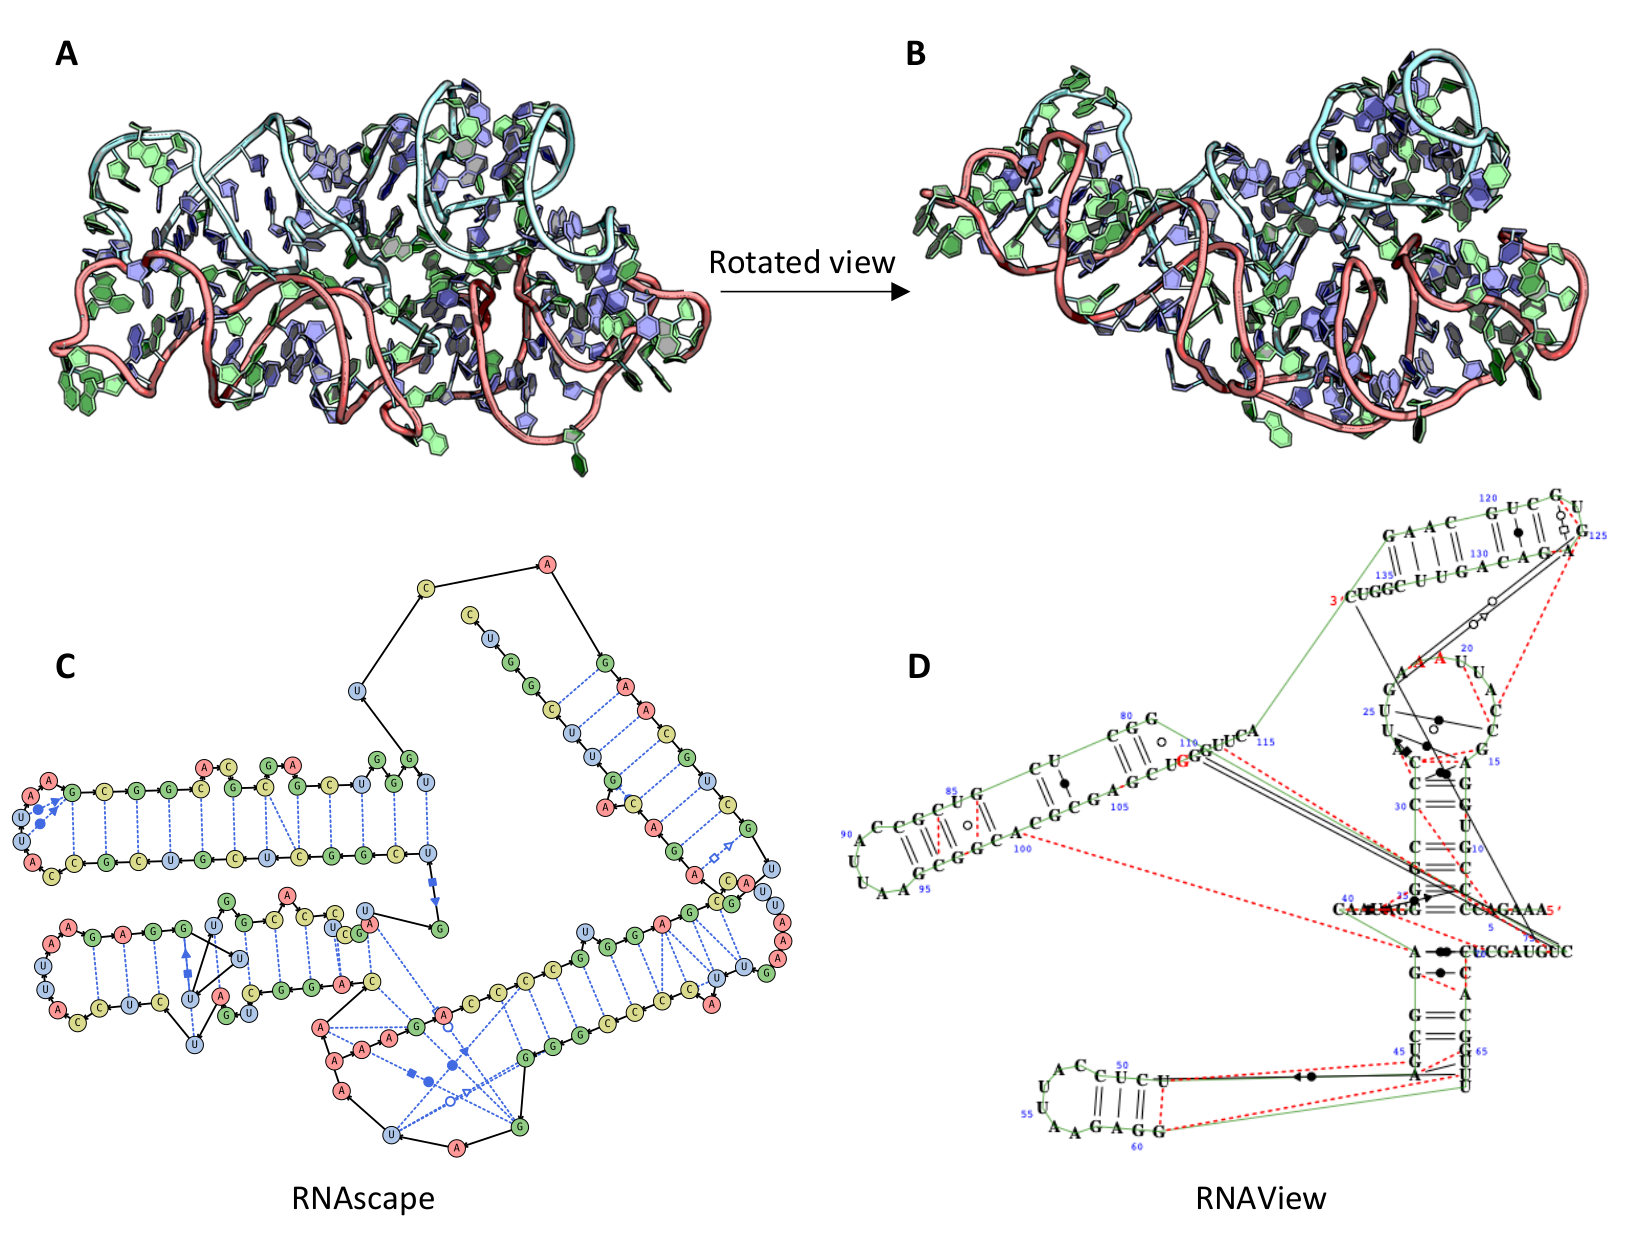
\includegraphics[width=\linewidth]{./rnascapefigs/figureS1.png}
 % archetecture.png: 1149x508 px, 72dpi, 40.53x17.92 cm, bb=0 0 1149 508
    \caption[Examples of continuous time prediction of ESC differentiation.]{\textbf{Examples of continuous time prediction of ESC differentiation.} Reconstruction (up to $t=6.8$) and future prediction (for $t>6.8$) for 4 example genes by a  latent ODE \citep{chen2018neural} trained on ESC data \citep{Klein2015} for 1000000 iterations, showing a good fit for the initial timepoints, but underfitting for the later timepoints.}
  \label{fig:rnascapeS1}
\end{figure}
\end{center}

\begin{center}
\begin{figure}[H]
  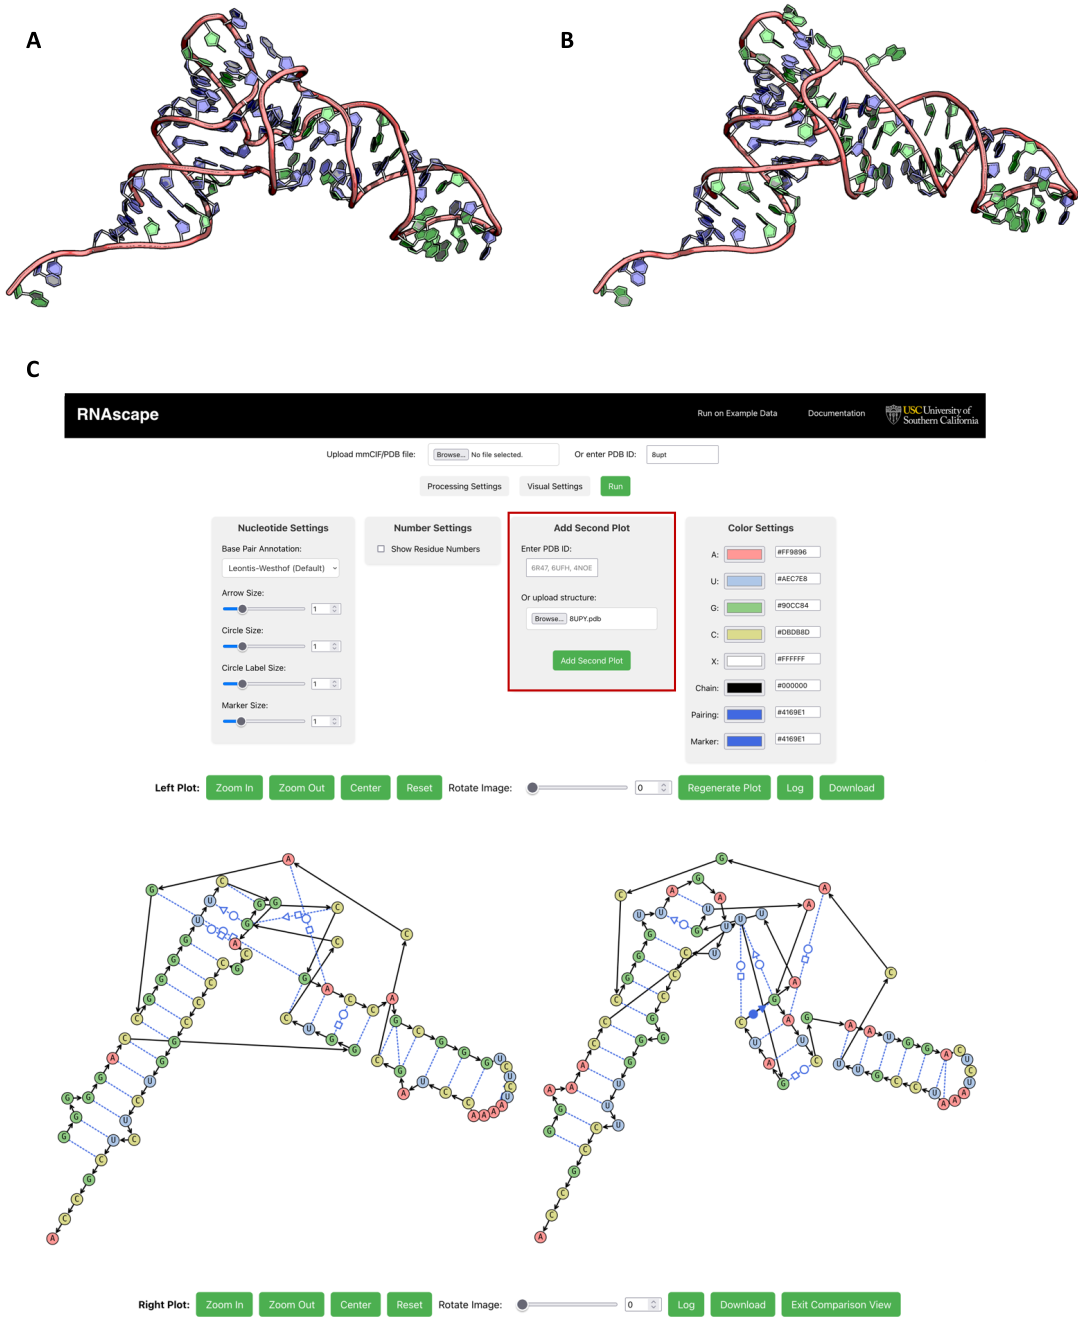
\includegraphics[width=\linewidth]{./rnascapefigs/figureS2.png}
 % archetecture.png: 1149x508 px, 72dpi, 40.53x17.92 cm, bb=0 0 1149 508
    \caption[Examples of continuous time prediction of ESC differentiation.]{\textbf{Examples of continuous time prediction of ESC differentiation.} Reconstruction (up to $t=6.8$) and future prediction (for $t>6.8$) for 4 example genes by a  latent ODE \citep{chen2018neural} trained on ESC data \citep{Klein2015} for 1000000 iterations, showing a good fit for the initial timepoints, but underfitting for the later timepoints.}
  \label{fig:rnascapeS2}
\end{figure}
\end{center}

\begin{center}
\begin{figure}[H]
  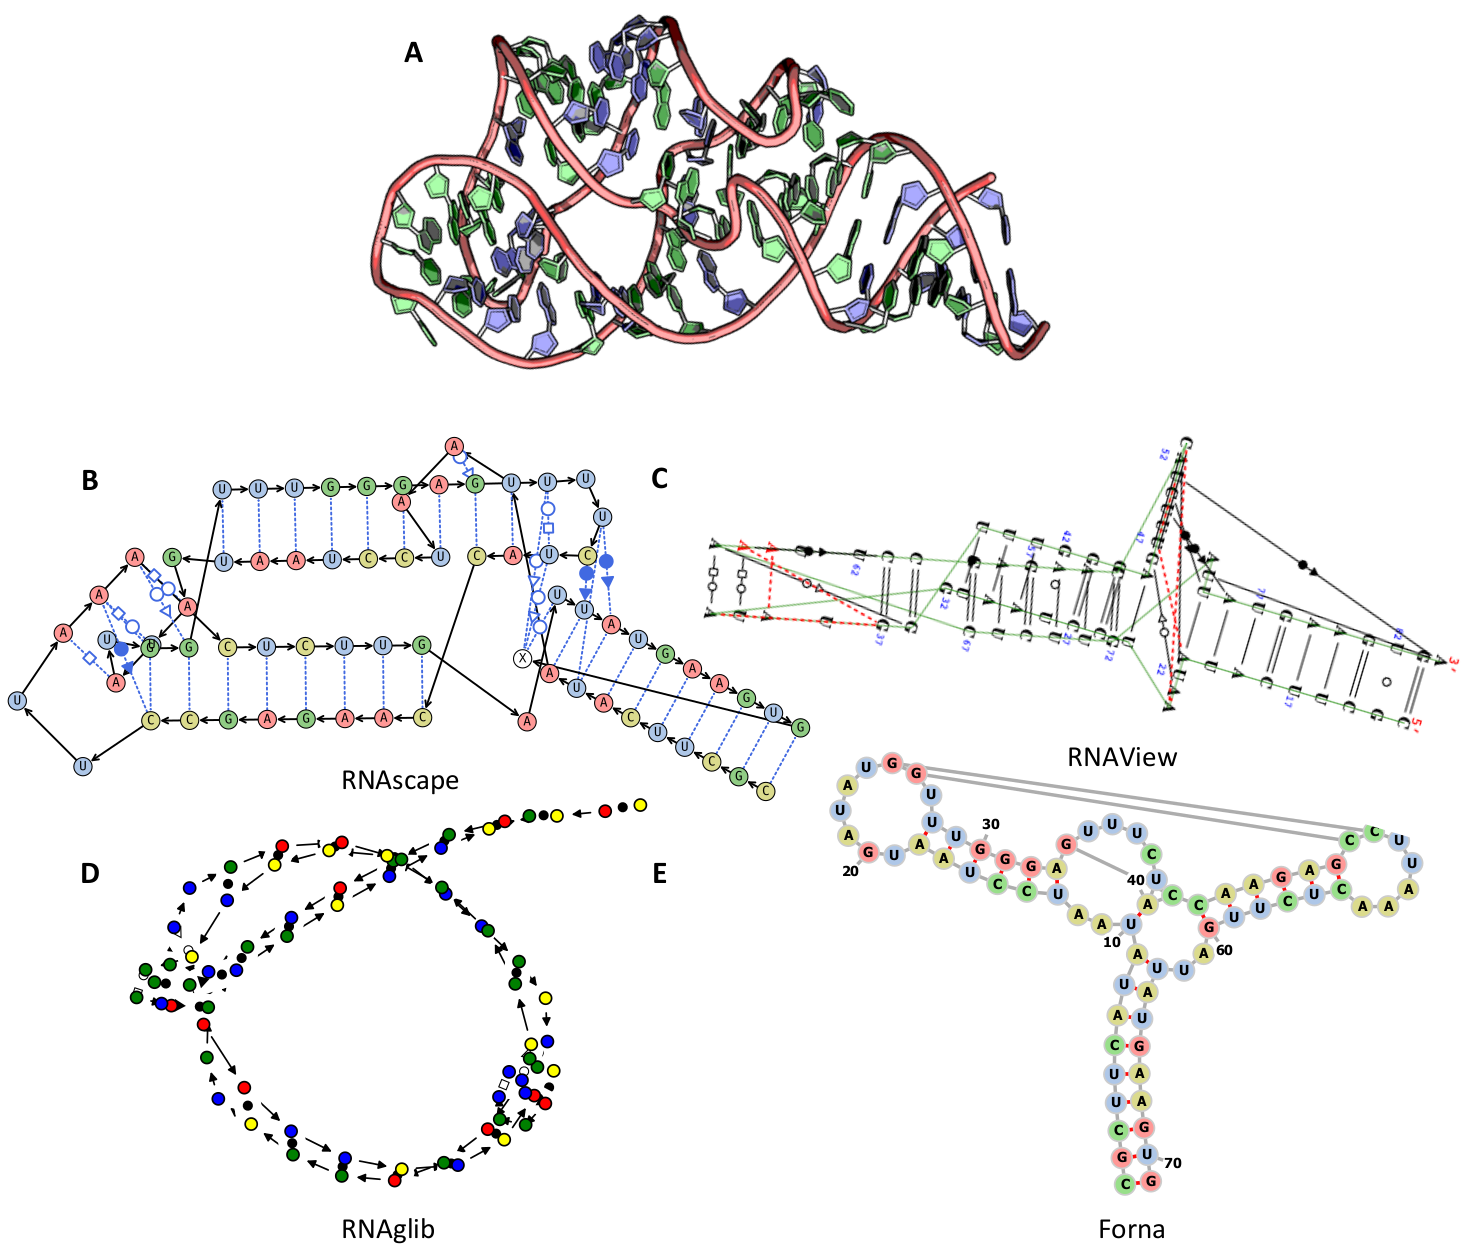
\includegraphics[width=\linewidth]{./rnascapefigs/figureS3.png}
 % archetecture.png: 1149x508 px, 72dpi, 40.53x17.92 cm, bb=0 0 1149 508
    \caption[Examples of continuous time prediction of ESC differentiation.]{\textbf{Examples of continuous time prediction of ESC differentiation.} Reconstruction (up to $t=6.8$) and future prediction (for $t>6.8$) for 4 example genes by a  latent ODE \citep{chen2018neural} trained on ESC data \citep{Klein2015} for 1000000 iterations, showing a good fit for the initial timepoints, but underfitting for the later timepoints.}
  \label{fig:rnascapeS3}
\end{figure}
\end{center}

%% DeepPBS SUPP FIGURES
\begin{center}
\begin{figure}[H]
  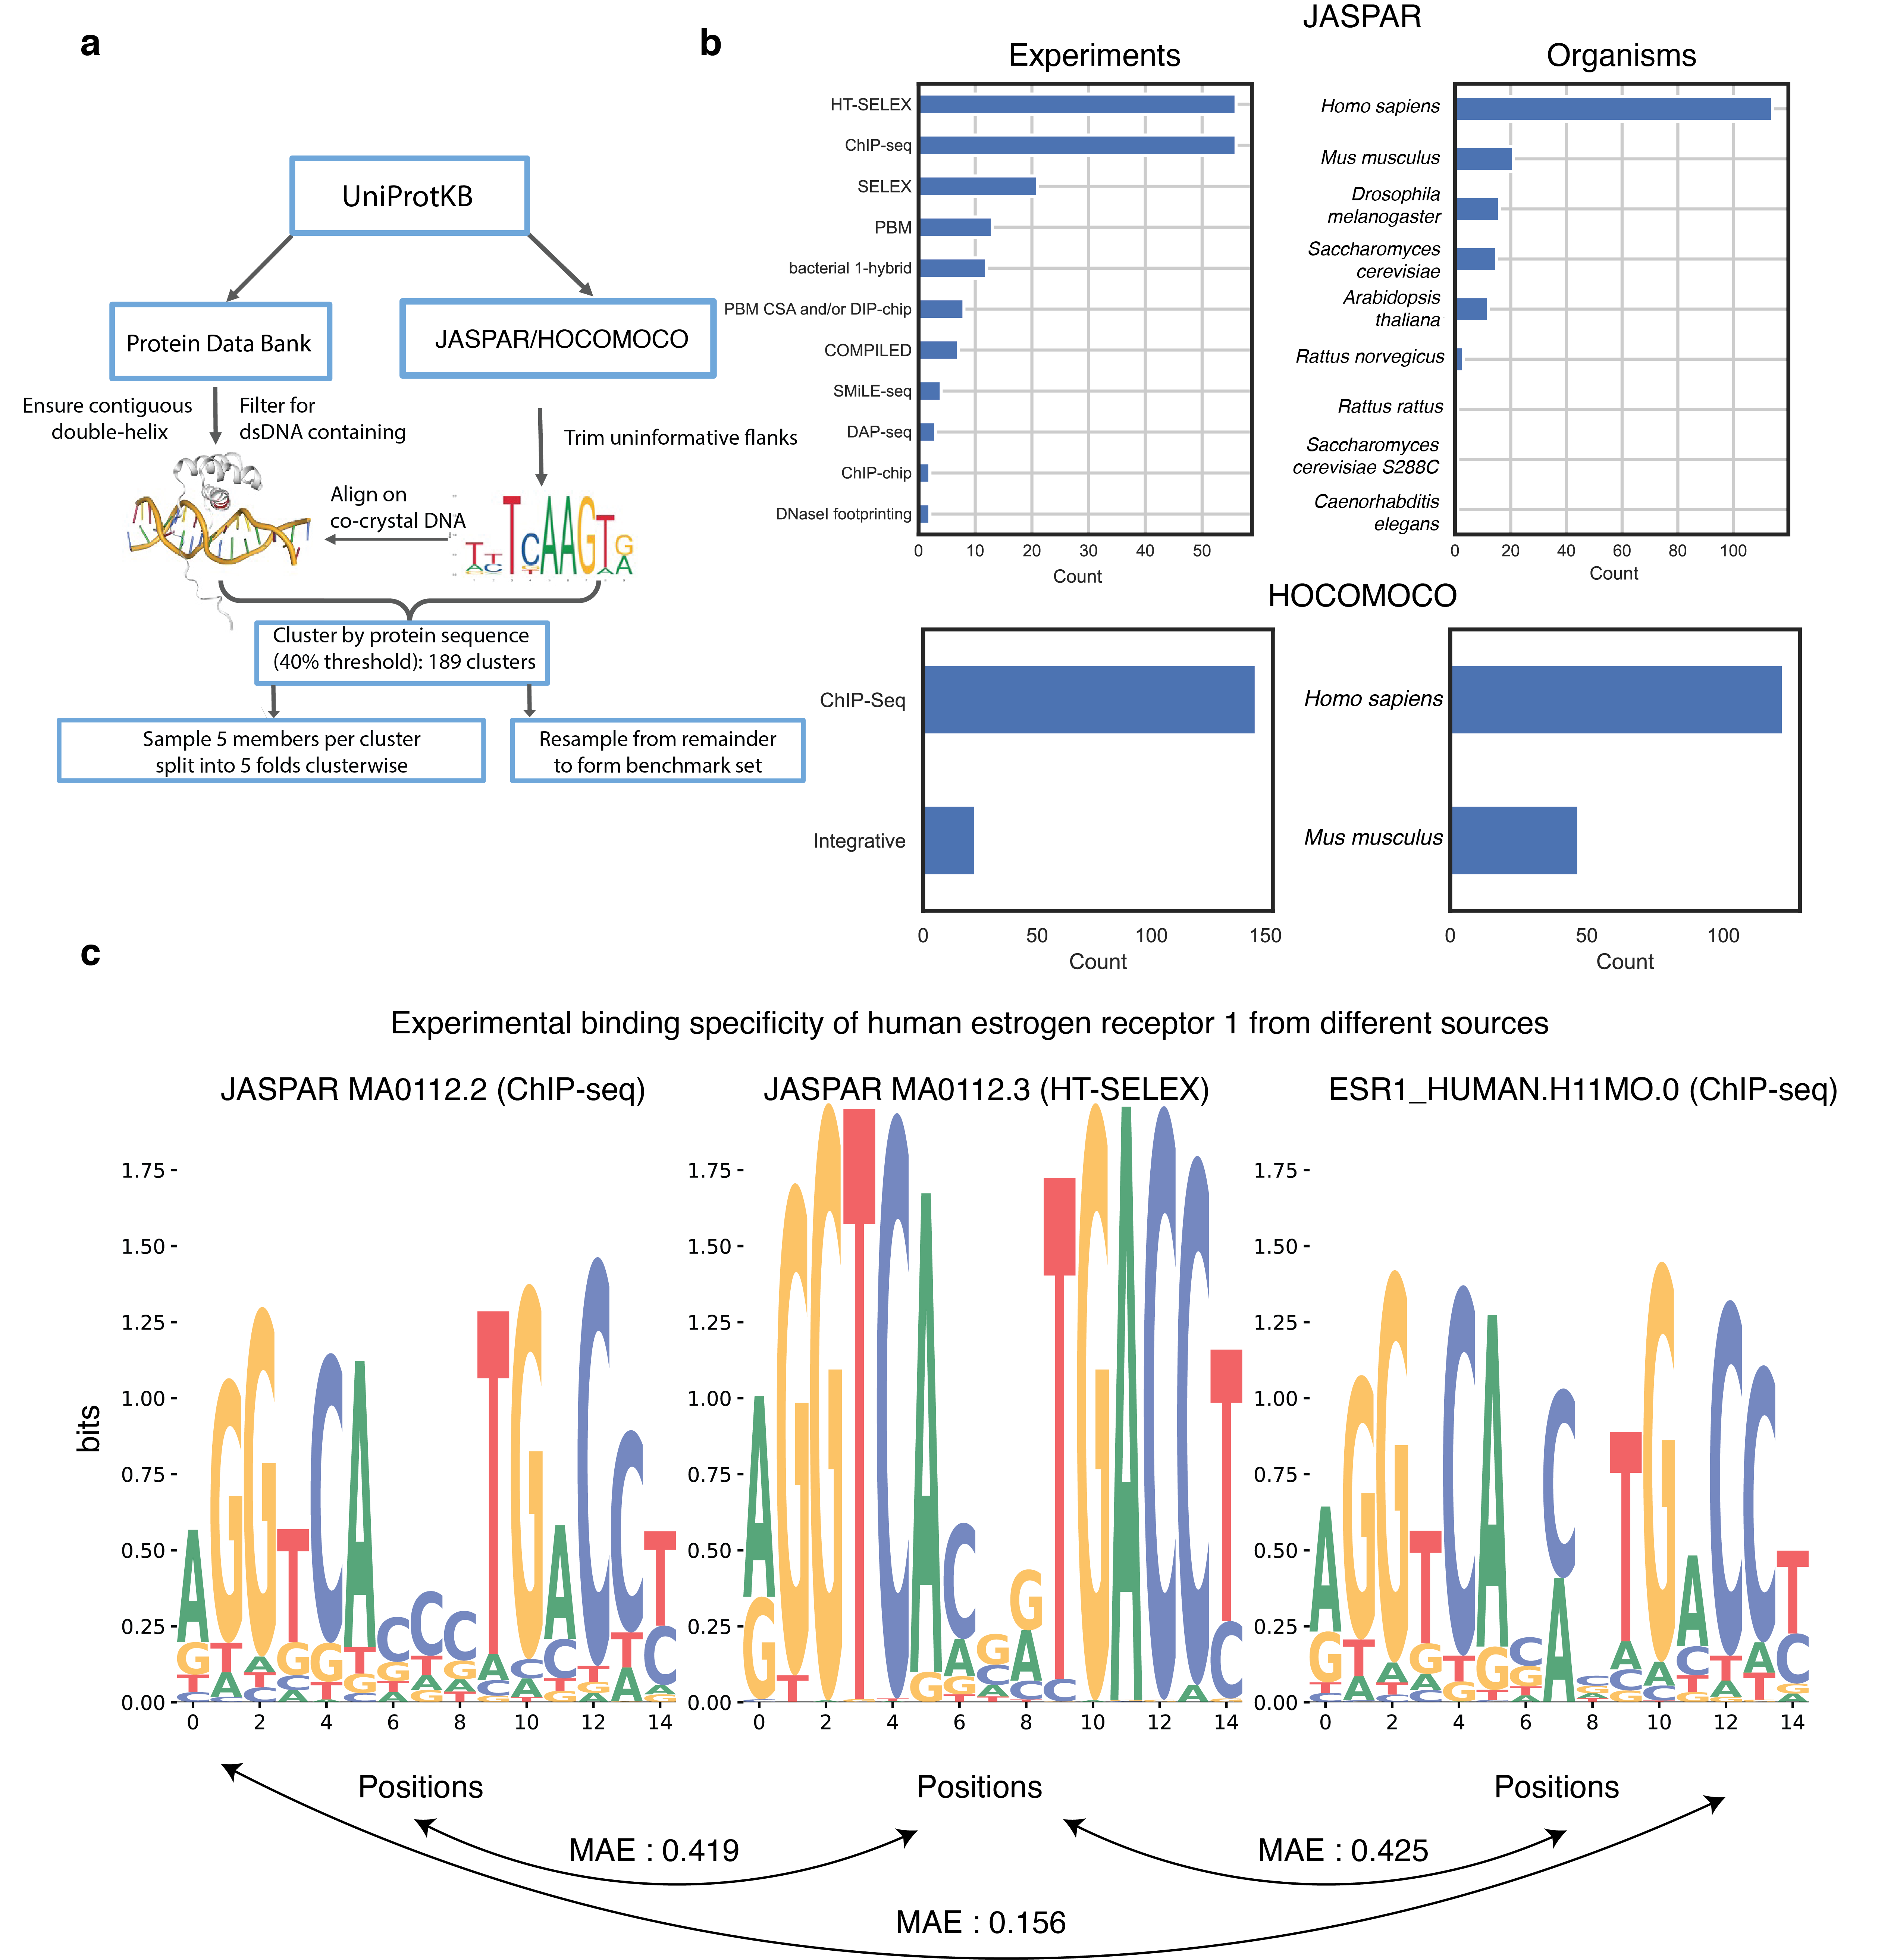
\includegraphics[width=\linewidth]{./pdnafigs/figS1.png}
 % archetecture.png: 1149x508 px, 72dpi, 40.53x17.92 cm, bb=0 0 1149 508
    \caption[Examples of continuous time prediction of ESC differentiation.]{\textbf{Examples of continuous time prediction of ESC differentiation.} Reconstruction (up to $t=6.8$) and future prediction (for $t>6.8$) for 4 example genes by a  latent ODE \citep{chen2018neural} trained on ESC data \citep{Klein2015} for 1000000 iterations, showing a good fit for the initial timepoints, but underfitting for the later timepoints.}
  \label{fig:pdnaS1}
\end{figure}
\end{center}

\begin{center}
\begin{figure}[H]
  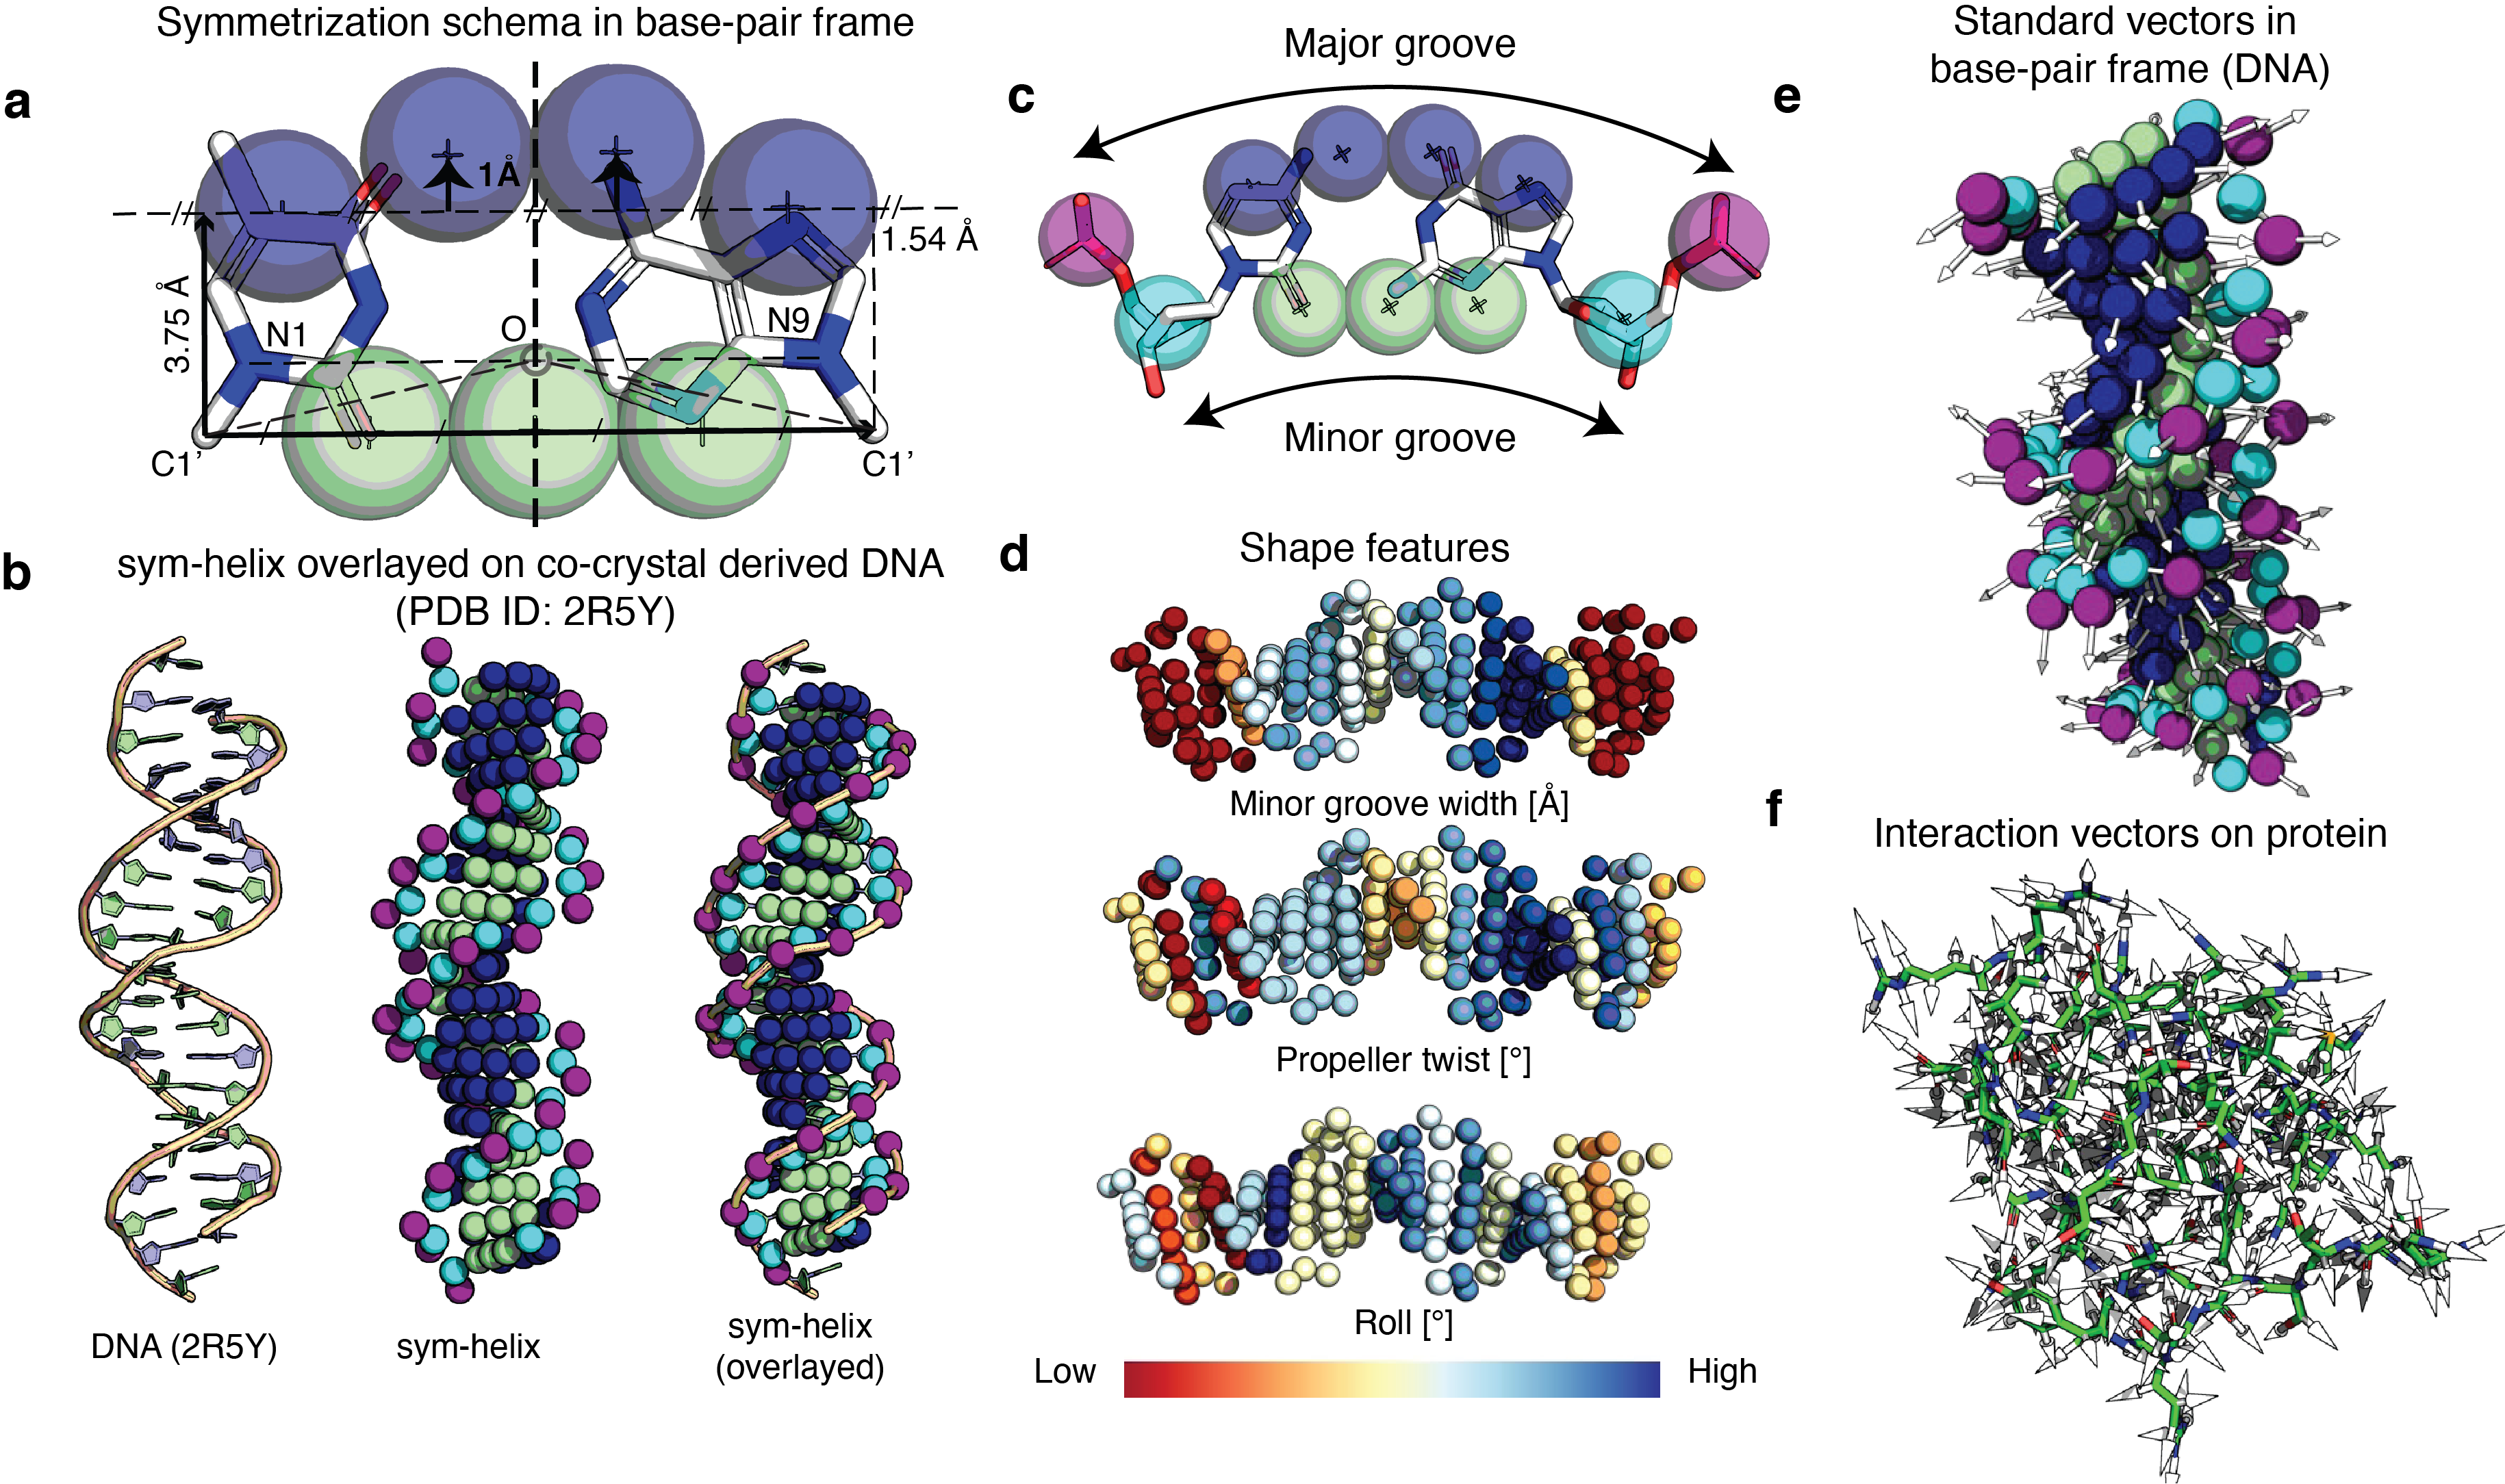
\includegraphics[width=\linewidth]{./pdnafigs/figS2.png}
 % archetecture.png: 1149x508 px, 72dpi, 40.53x17.92 cm, bb=0 0 1149 508
    \caption[Examples of continuous time prediction of ESC differentiation.]{\textbf{Examples of continuous time prediction of ESC differentiation.} Reconstruction (up to $t=6.8$) and future prediction (for $t>6.8$) for 4 example genes by a  latent ODE \citep{chen2018neural} trained on ESC data \citep{Klein2015} for 1000000 iterations, showing a good fit for the initial timepoints, but underfitting for the later timepoints.}
  \label{fig:pdnaS2}
\end{figure}
\end{center}

\begin{center}
\begin{figure}[H]
  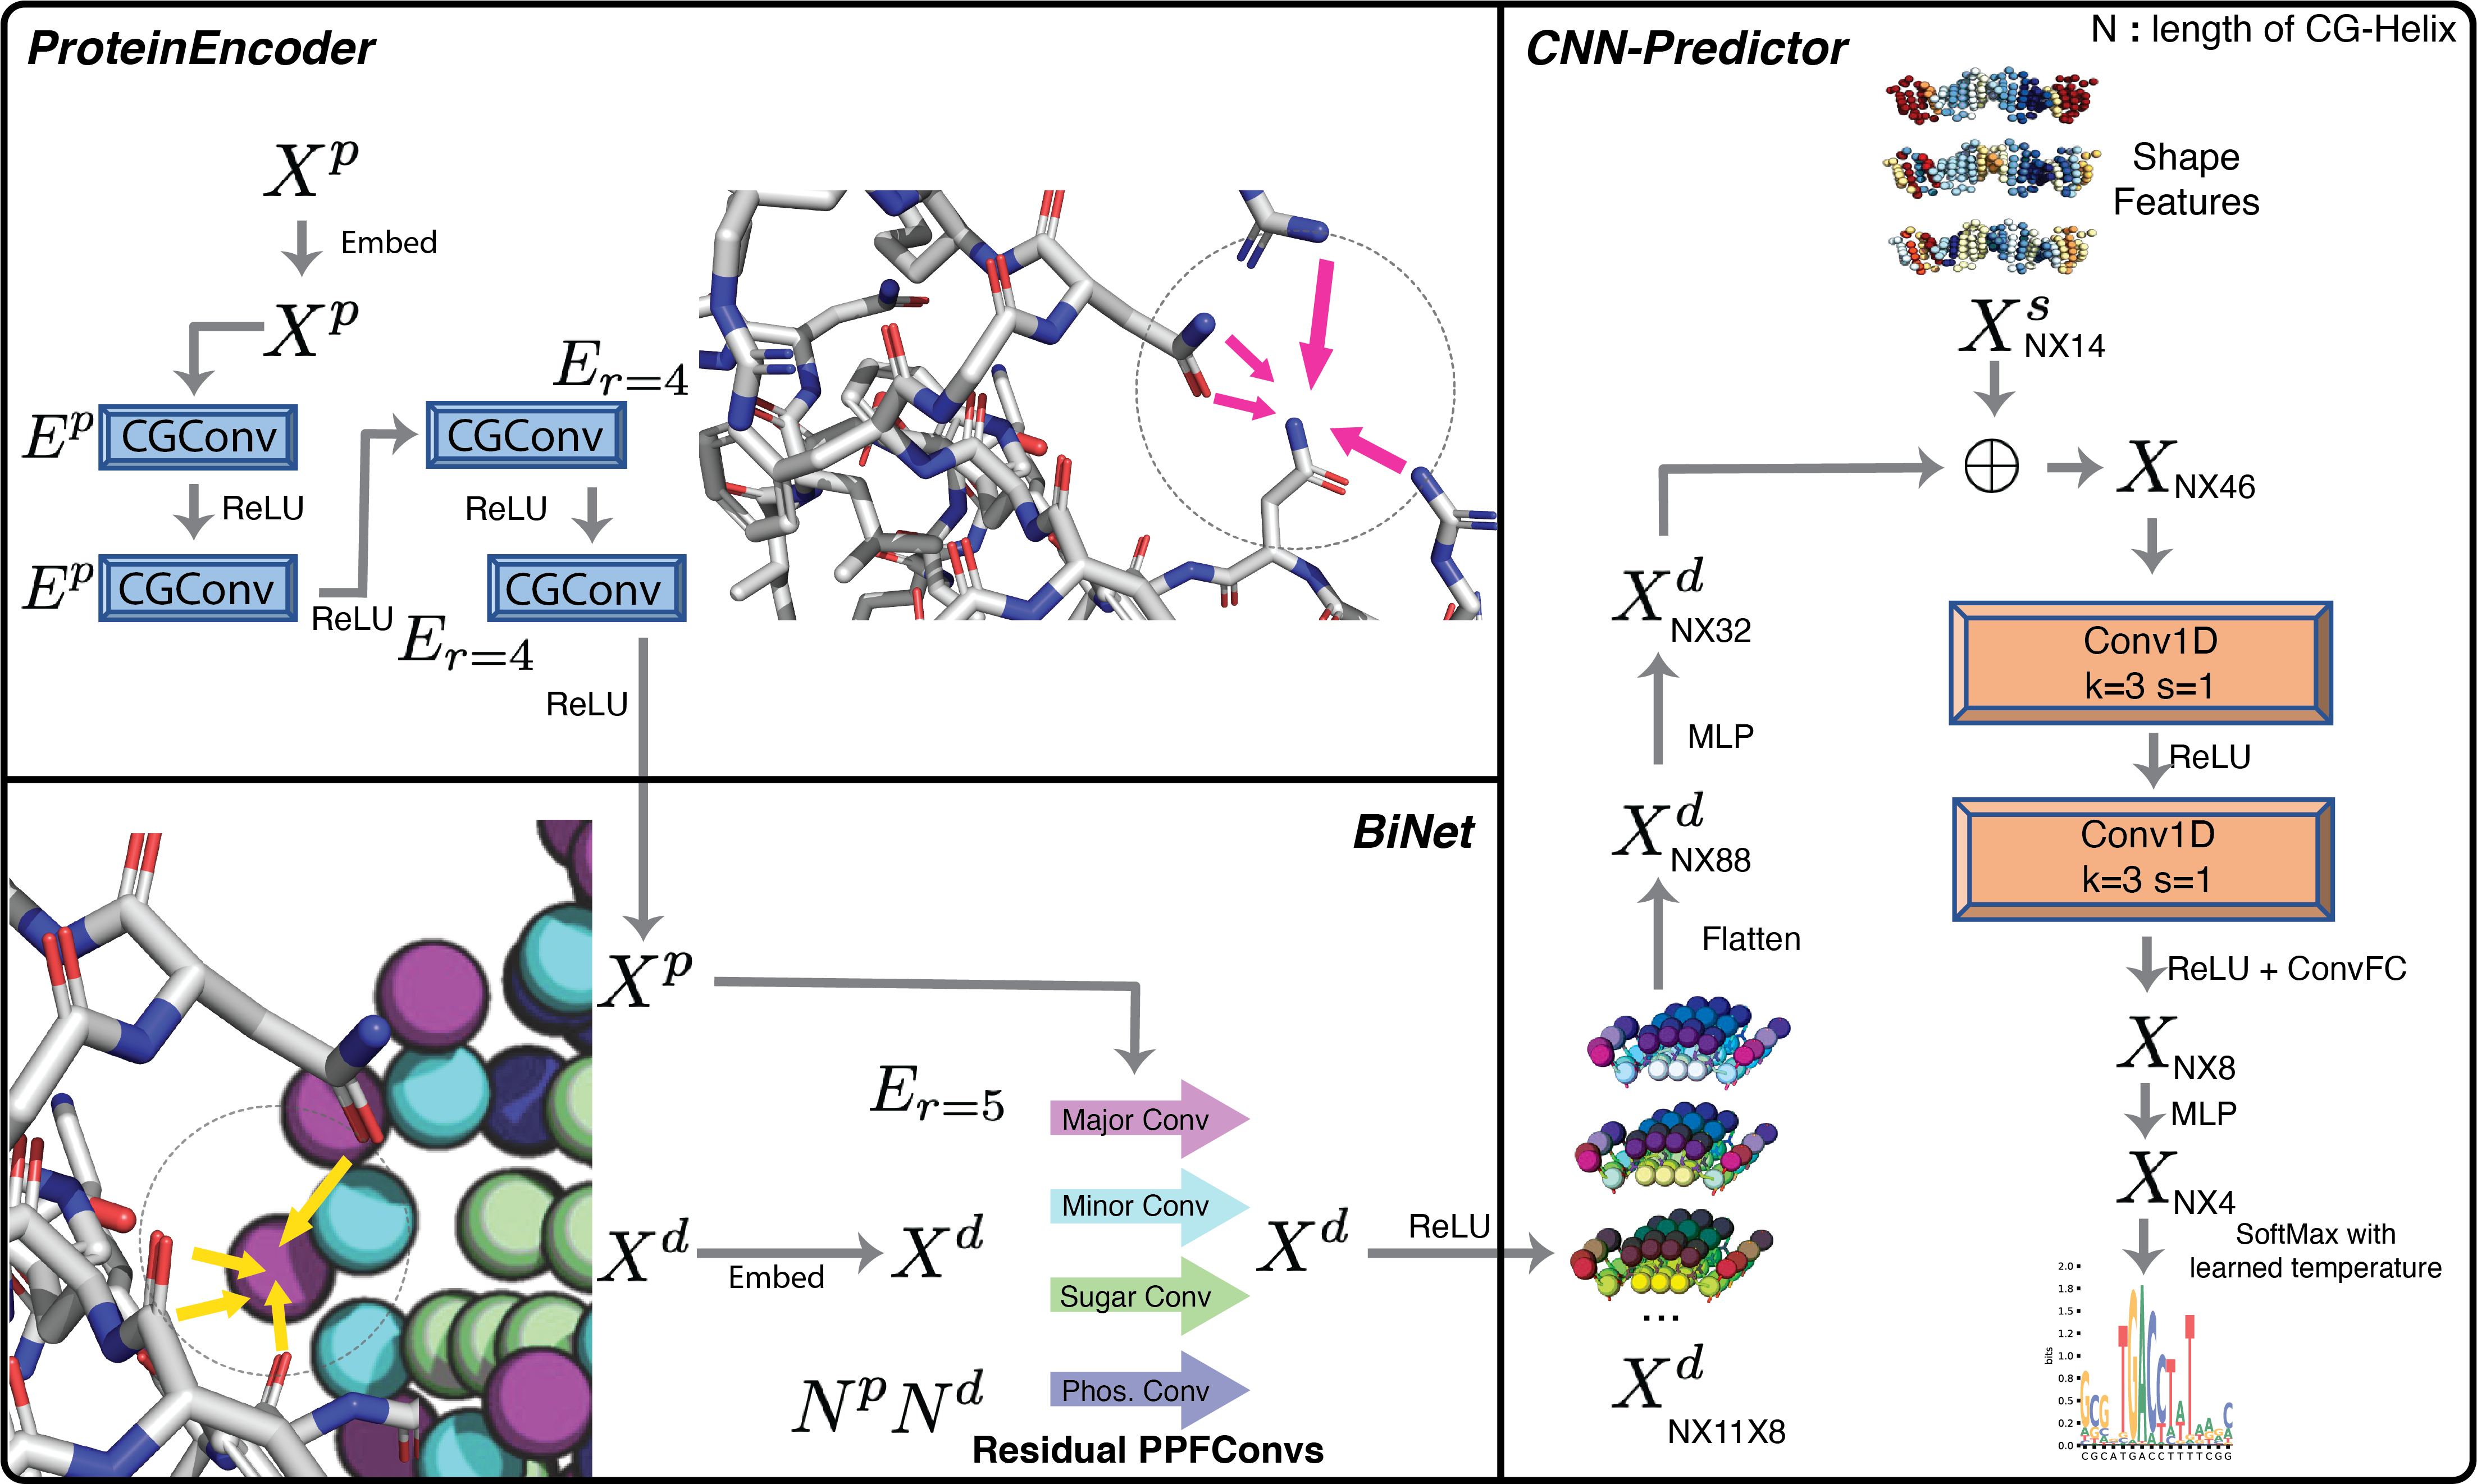
\includegraphics[width=\linewidth]{./pdnafigs/figS3.png}
 % archetecture.png: 1149x508 px, 72dpi, 40.53x17.92 cm, bb=0 0 1149 508
    \caption[Examples of continuous time prediction of ESC differentiation.]{\textbf{Examples of continuous time prediction of ESC differentiation.} Reconstruction (up to $t=6.8$) and future prediction (for $t>6.8$) for 4 example genes by a  latent ODE \citep{chen2018neural} trained on ESC data \citep{Klein2015} for 1000000 iterations, showing a good fit for the initial timepoints, but underfitting for the later timepoints.}
  \label{fig:pdnaS3}
\end{figure}
\end{center}

\begin{center}
\begin{figure}[H]
  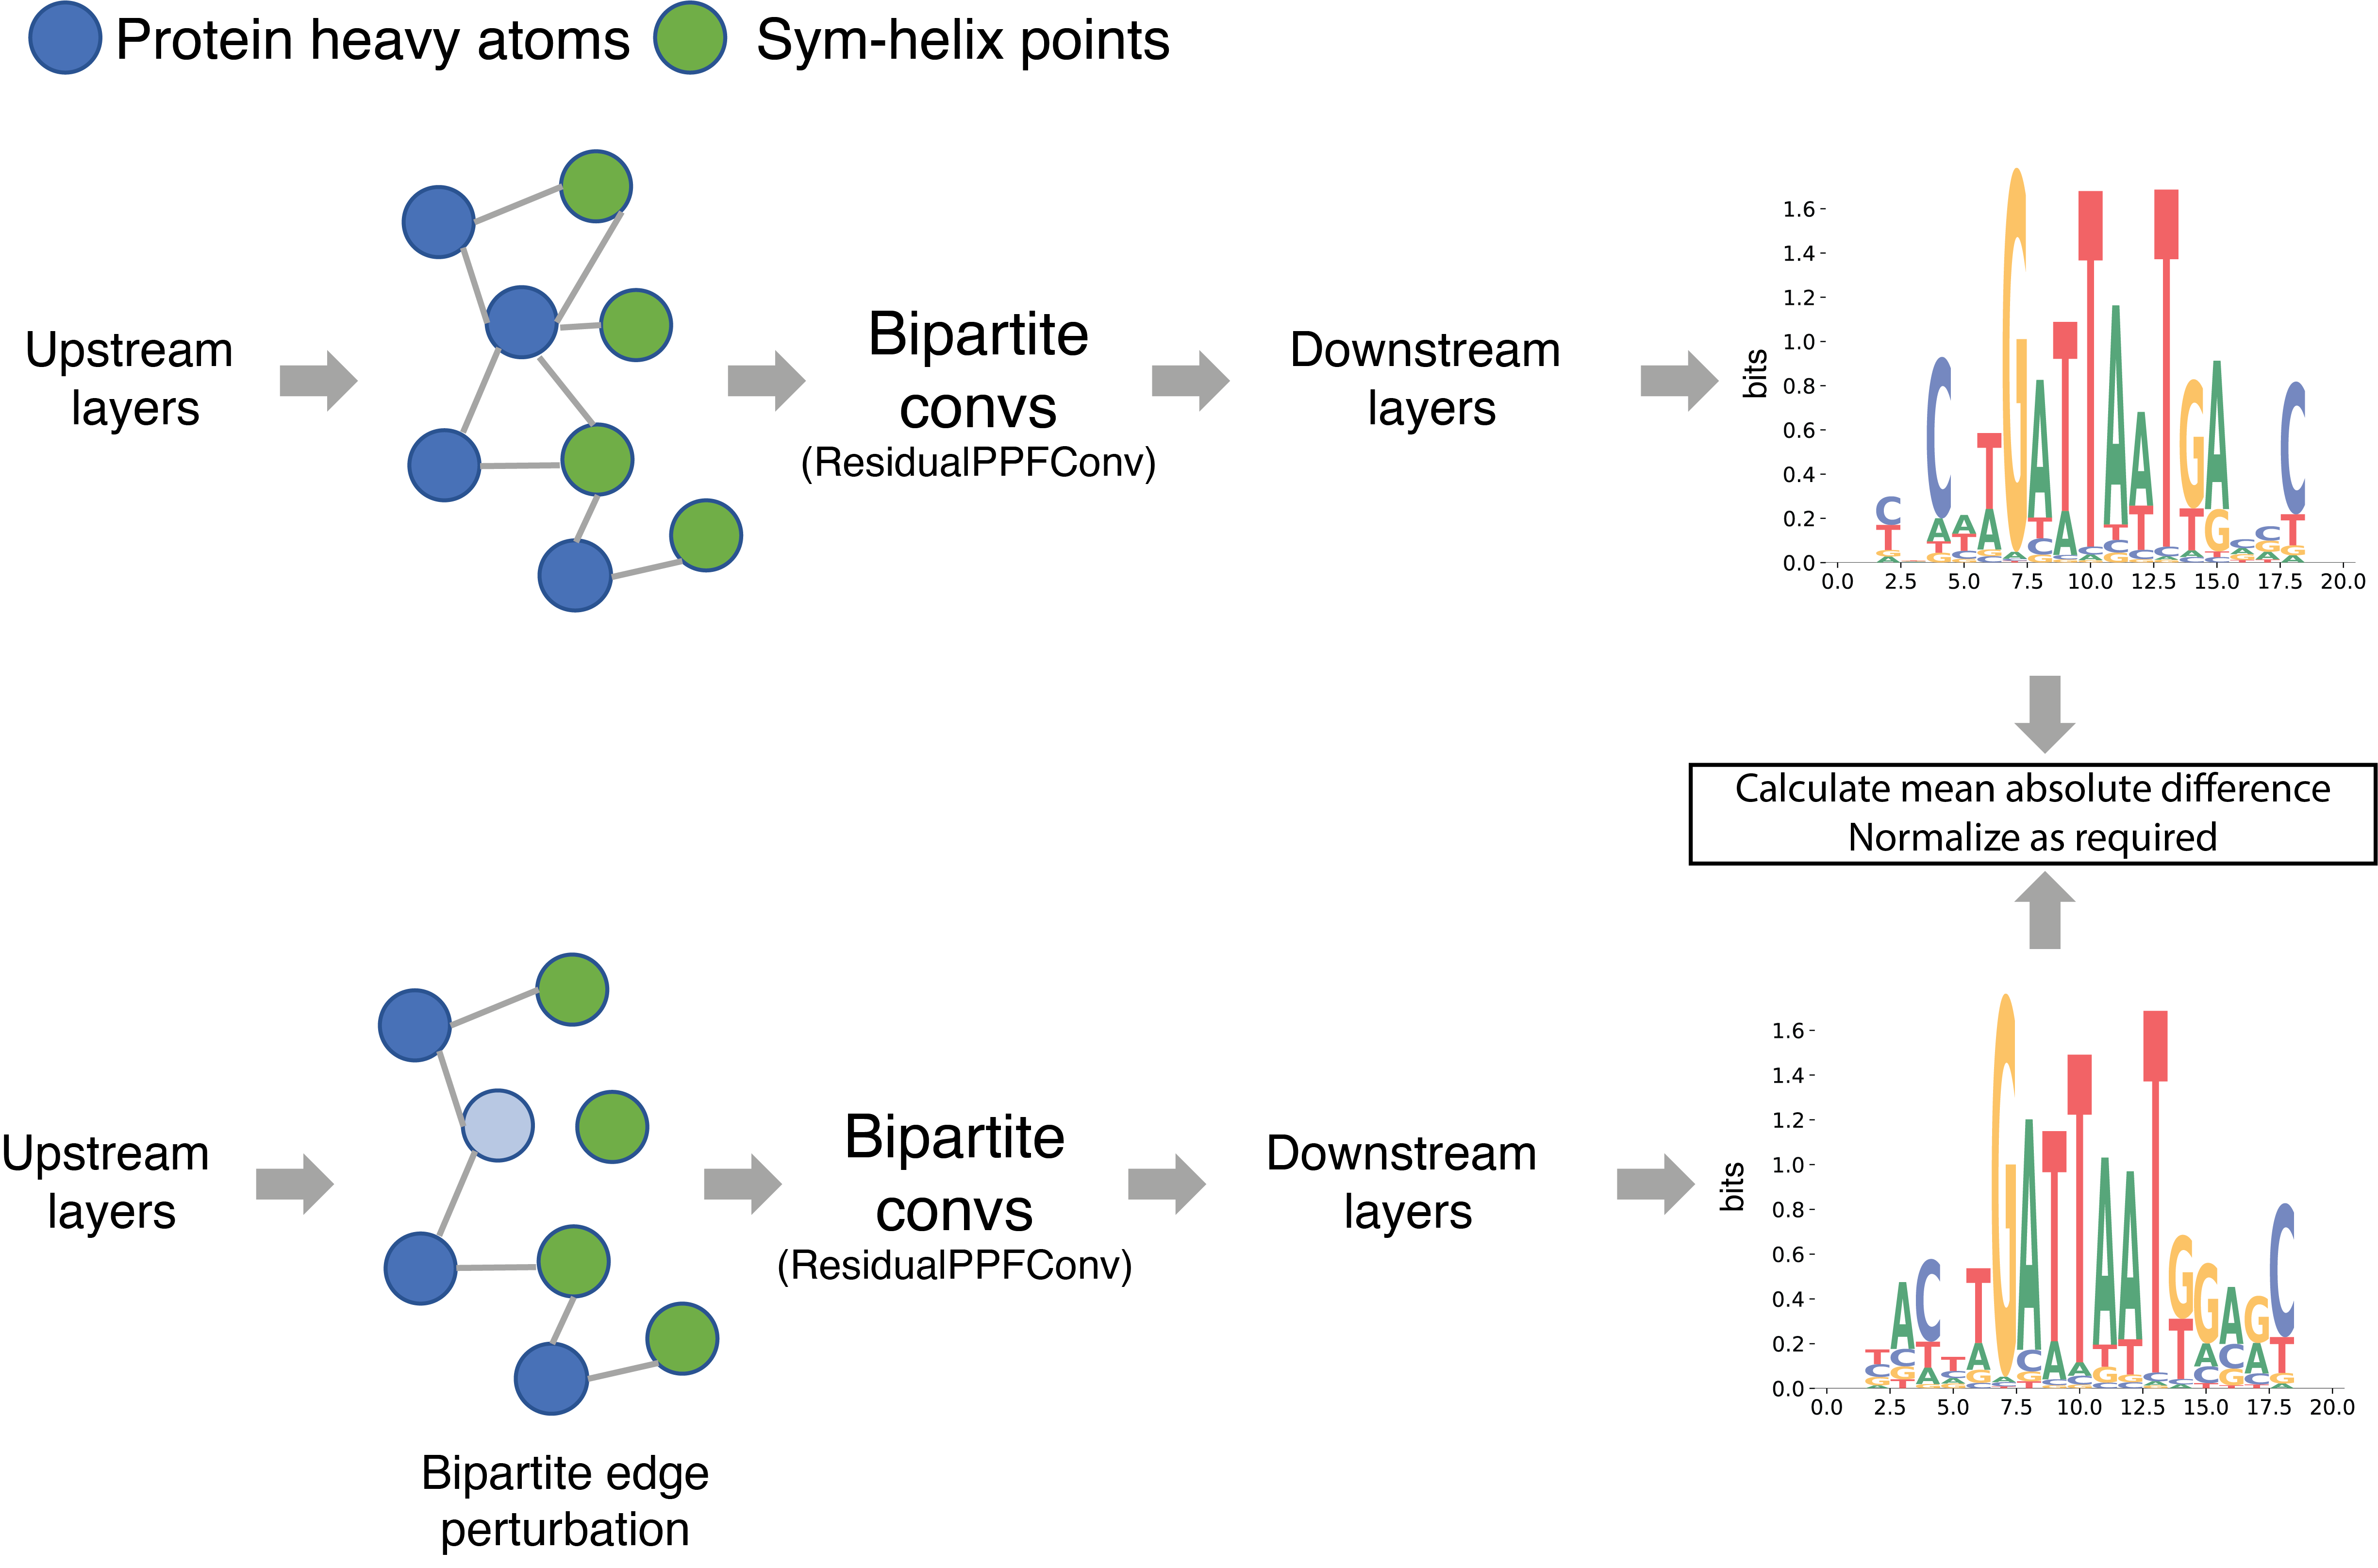
\includegraphics[width=\linewidth]{./pdnafigs/figS4.png}
 % archetecture.png: 1149x508 px, 72dpi, 40.53x17.92 cm, bb=0 0 1149 508
    \caption[Examples of continuous time prediction of ESC differentiation.]{\textbf{Examples of continuous time prediction of ESC differentiation.} Reconstruction (up to $t=6.8$) and future prediction (for $t>6.8$) for 4 example genes by a  latent ODE \citep{chen2018neural} trained on ESC data \citep{Klein2015} for 1000000 iterations, showing a good fit for the initial timepoints, but underfitting for the later timepoints.}
  \label{fig:pdnaS4}
\end{figure}
\end{center}

\begin{center}
\begin{figure}[H]
  \includegraphics[width=\linewidth]{./pdnafigs/figS5.png}
 % archetecture.png: 1149x508 px, 72dpi, 40.53x17.92 cm, bb=0 0 1149 508
    \caption[Examples of continuous time prediction of ESC differentiation.]{\textbf{Examples of continuous time prediction of ESC differentiation.} Reconstruction (up to $t=6.8$) and future prediction (for $t>6.8$) for 4 example genes by a  latent ODE \citep{chen2018neural} trained on ESC data \citep{Klein2015} for 1000000 iterations, showing a good fit for the initial timepoints, but underfitting for the later timepoints.}
  \label{fig:pdnaS5}
\end{figure}
\end{center}

\begin{center}
\begin{figure}[H]
  \includegraphics[width=\linewidth]{./pdnafigs/figS6.png}
 % archetecture.png: 1149x508 px, 72dpi, 40.53x17.92 cm, bb=0 0 1149 508
    \caption[Examples of continuous time prediction of ESC differentiation.]{\textbf{Examples of continuous time prediction of ESC differentiation.} Reconstruction (up to $t=6.8$) and future prediction (for $t>6.8$) for 4 example genes by a  latent ODE \citep{chen2018neural} trained on ESC data \citep{Klein2015} for 1000000 iterations, showing a good fit for the initial timepoints, but underfitting for the later timepoints.}
  \label{fig:pdnaS6}
\end{figure}
\end{center}

\begin{center}
\begin{figure}[H]
  \includegraphics[width=\linewidth]{./pdnafigs/figS7.png}
 % archetecture.png: 1149x508 px, 72dpi, 40.53x17.92 cm, bb=0 0 1149 508
    \caption[Examples of continuous time prediction of ESC differentiation.]{\textbf{Examples of continuous time prediction of ESC differentiation.} Reconstruction (up to $t=6.8$) and future prediction (for $t>6.8$) for 4 example genes by a  latent ODE \citep{chen2018neural} trained on ESC data \citep{Klein2015} for 1000000 iterations, showing a good fit for the initial timepoints, but underfitting for the later timepoints.}
  \label{fig:pdnaS7}
\end{figure}
\end{center}

\begin{center}
\begin{figure}[H]
  \includegraphics[width=\linewidth]{./pdnafigs/figS8.png}
 % archetecture.png: 1149x508 px, 72dpi, 40.53x17.92 cm, bb=0 0 1149 508
    \caption[Examples of continuous time prediction of ESC differentiation.]{\textbf{Examples of continuous time prediction of ESC differentiation.} Reconstruction (up to $t=6.8$) and future prediction (for $t>6.8$) for 4 example genes by a  latent ODE \citep{chen2018neural} trained on ESC data \citep{Klein2015} for 1000000 iterations, showing a good fit for the initial timepoints, but underfitting for the later timepoints.}
  \label{fig:pdnaS8}
\end{figure}
\end{center}

\begin{center}
\begin{figure}[H]
  \includegraphics[width=\linewidth]{./pdnafigs/figS9.png}
 % archetecture.png: 1149x508 px, 72dpi, 40.53x17.92 cm, bb=0 0 1149 508
    \caption[Examples of continuous time prediction of ESC differentiation.]{\textbf{Examples of continuous time prediction of ESC differentiation.} Reconstruction (up to $t=6.8$) and future prediction (for $t>6.8$) for 4 example genes by a  latent ODE \citep{chen2018neural} trained on ESC data \citep{Klein2015} for 1000000 iterations, showing a good fit for the initial timepoints, but underfitting for the later timepoints.}
  \label{fig:pdnaS9}
\end{figure}
\end{center}

\begin{center}
\begin{figure}[H]
  \includegraphics[width=\linewidth]{./pdnafigs/figS10.png}
 % archetecture.png: 1149x508 px, 72dpi, 40.53x17.92 cm, bb=0 0 1149 508
    \caption[Examples of continuous time prediction of ESC differentiation.]{\textbf{Examples of continuous time prediction of ESC differentiation.} Reconstruction (up to $t=6.8$) and future prediction (for $t>6.8$) for 4 example genes by a  latent ODE \citep{chen2018neural} trained on ESC data \citep{Klein2015} for 1000000 iterations, showing a good fit for the initial timepoints, but underfitting for the later timepoints.}
  \label{fig:pdnaS10}
\end{figure}
\end{center}

\begin{center}
\begin{figure}[H]
  \includegraphics[width=\linewidth]{./pdnafigs/figS11.png}
 % archetecture.png: 1149x508 px, 72dpi, 40.53x17.92 cm, bb=0 0 1149 508
    \caption[Examples of continuous time prediction of ESC differentiation.]{\textbf{Examples of continuous time prediction of ESC differentiation.} Reconstruction (up to $t=6.8$) and future prediction (for $t>6.8$) for 4 example genes by a  latent ODE \citep{chen2018neural} trained on ESC data \citep{Klein2015} for 1000000 iterations, showing a good fit for the initial timepoints, but underfitting for the later timepoints.}
  \label{fig:pdnaS11}
\end{figure}
\end{center}

\begin{center}
\begin{figure}[H]
  \includegraphics[width=\linewidth]{./pdnafigs/figS12.png}
 % archetecture.png: 1149x508 px, 72dpi, 40.53x17.92 cm, bb=0 0 1149 508
    \caption[Examples of continuous time prediction of ESC differentiation.]{\textbf{Examples of continuous time prediction of ESC differentiation.} Reconstruction (up to $t=6.8$) and future prediction (for $t>6.8$) for 4 example genes by a  latent ODE \citep{chen2018neural} trained on ESC data \citep{Klein2015} for 1000000 iterations, showing a good fit for the initial timepoints, but underfitting for the later timepoints.}
  \label{fig:pdnaS12}
\end{figure}
\end{center}

% Appendices
\phantomsection
\addcontentsline{toc}{chapter}{Appendices}%
\markboth{Appendices}{Appendices}%
\chapter*{Appendices}
\section*{Appendix A}
\addcontentsline{toc}{section}{Appendix A}%
\renewcommand\thesection{\Alph{section}}
\renewcommand*{\thesubsection}{\Alph{section}.\arabic{subsection}}
\begingroup
\numberwithin{equation}{section}
% Appendix source files
%\section{A Long Proof}
\label{app:long_proof}

\subsection{Part one}
A long proof that nobody is gonna read goes here.

\subsection{Part two}
Part two of the long proof that nobody is gonna read goes here.

\Blindtext[1]

%
%SetFonts


%\date{}							% Activate to display a given date or no date

\section*{Detailed calculation of the CCRF layer update}
Starting from the mean field variational inference result in eq. \ref{mean_field_VI_result} we have, %\red{(Kr\"{a}henb\"{u}hl, 2012)} we have,
\label{crf_detailed}
\begin{equation}
Q_i (H_i) \simeq \frac{1}{Z} \exp \left ( - \alpha || H_i - B_i ||^2  - \beta \sum_{j \in \mathcal{N}(i)} g_{ij} \int_{-\infty}^{\infty} Q(H_j) ||H_i - H_j ||^2 d H_j\right )
\end{equation}

where $H_i, B_i, H_j \in \mathbb{R}^N$. Evaluating this component-wise and using the definition of the $\ell_2$ norm, we can write the energy $E(H_i)$ as

\begin{equation}
E(H_i) = \alpha \sum_n^N (H_{in} - B_{in})^2 + \beta \sum_{j \in \mathcal{N}(i)} g_{ij} \sum_n^N \int_{-\infty}^{\infty} \cdots \int_{-\infty}^{\infty} Q(H_j) (H_{in} - H_{jn})^2 d H_{j1}\cdots dH_{jN}
\end{equation}.

Focusing on the inner most summation of second term, since each component of $H_i$ and $H_j$ is
independent (by eq. 10 of \citet{gao2019conditional}), we can write $Q(H_j) = \Pi_{k=1}^N Q_{jk}(H_{jk})$ and assume that each $Q_{jk}$ is individually normalized. The summation then becomes

\begin{multline}
 \sum_n^N \int_{-\infty}^{\infty}  Q(H_j) (H_{in} - H_{jn})^2 d H_{j1}\cdots dH_{jN} \\
= \sum_n^N \int_{-\infty}^{\infty} (H_{in} - H_{jn})^2  \Pi_{k=1}^N Q_{jk}(H_{jk}) d H_{jk} \\
= \sum_n^N \int_{-\infty}^{\infty} (H_{in} - H_{jn})^2  Q_{jn}(H_{jn}) d H_{jn}\int_{-\infty}^{\infty}  \Pi_{k\neq n}^N Q_{jk}(H_{jk}) d H_{jk} \\
\end{multline} 

where the last step follows because all the $Q_{jk}$'s integrate to 1. Therefore, we have that the energy is given by

\begin{equation}
E(H_i) = \sum_n^N \left [ \alpha (H_{in} - B_{in})^2 + \beta \sum_{j \in \mathcal{N}(i)} g_{ij}  \int_{-\infty}^{\infty} (H_{in} - H_{jn})^2  Q_{jn}(H_{jn}) d H_{jn} \right ]
\end{equation}

Taking the derivative of $E(H_i)$ with respect to the $k$ component of $H_i$ we have

\begin{multline}
\frac{\partial E(H_i)} {\partial H_{ik}} = 2\alpha (H_{ik} - B_{ik}) + \beta \sum_{j \in \mathcal{N}(i)} g_{ij} \int_{-\infty}^{\infty} 2 (H_{ik} - H_{jk})  Q_{jn}(H_{jk}) d H_{jk} \\
= 2\alpha (H_{ik} - B_{ik}) + 2\beta \sum_{j \in \mathcal{N}(i)} g_{ij}  (H_{ik} - \int_{-\infty}^{\infty} H_{jk} Q_{jk}(H_{jk})d H_{jk})
\end{multline}

setting this equal to zero and solving for $H_i$ we have

\begin{equation}
H_{ik}^* = \frac{\alpha B_{ik} + \beta  \sum\limits_{j \in \mathcal{N}(i)} g_{ij} \mathbb{E}_{ H_{jk} \sim Q_{jk} } [H_{jk}]} {\alpha +  \beta  \sum \limits_{j \in \mathcal{N}(i)} g_{ij} }
\end{equation}
%%%%%%% Raktim's section %%%%%%%%%%%%%%%%
\section*{Proposed Algorithm}
Given initial states $B_i$ of the nodes, $H_i^0 = B_i$ maximizes $Q_i^0 = \frac{1}{Z_i^0}exp(-c||H_i^0 - B_i||^2)$. Now, we can use the above update equation and approximately     compute (at $t$ th iteration) $H_i^{t+1}$ (maximising $Q_i^{t+1})$ using $H_i^t$ and so forth until convergence (i.e. upto some iteration K, after which $Q_i^t$ and $Q_i^{t+1}$ are not very different and hence, so are $H_i^{T}$ and $H_i^{T+1}$).
\\
Update for iteration k:
\begin{equation}
 H_{i}^{t+1} = \frac{\alpha B_{i} + \beta  \sum\limits_{j \in \mathcal{N}(i)} (g_{ij} H_j^t)} {\alpha +  \beta  \sum \limits_{j \in \mathcal{N}(i)} g_{ij} }
\end{equation}

We can get the aggregated values $(\sum \limits_{j \in \mathcal{N}(i)} (g_{ij} H_j^t),\sum \limits_{j \in \mathcal{N}(i)} g_{ij})$ for $i$th node in a message passing step using $E, B_i$ and $H_i^t$ $\forall i$.
%\begin{pmialgorithm}[0.9\textwidth]{H}{ Mean Field CCRF Layer}\vskip-2ex
%	\label{algo:tk-means}
%	\begin{algorithmic}[1]
%		\REQUIRE  $B_i$  $\forall i$, $E$ (adjacency information)
%		\STATE Initialize $H_i^0 = B_i$ $\forall i$\COMMENT{$H_i^0$ maximizes $Q_i^0 = \frac{1}{Z_i^0}exp(-c||H_i^0 - B_i||^2)$}
%		\FOR[$T$ signifies convergence]{$t=0,1,2,...,T-1$} 
%        \STATE compute $(\sum \limits_{j \in \mathcal{N}(i)} (g_{ij} H_j^t),\sum \limits_{j \in \mathcal{N}(i)} g_{ij})$ \COMMENT{message passing}
%        \STATE $H_i^{t'} = \alpha B_{i} + \beta  \sum\limits_{j \in \mathcal{N}(i)} (g_{ij} H_j^t)$ 
%        \STATE $H_i^{t+1} = H_i^{t'} / (\alpha +  \beta  \sum \limits_{j \in \mathcal{N}(i)} g_{ij} )$ 
%		\ENDFOR 
%		\STATE $H_i^* = H_i^T$
%		\RETURN $H_i^*$
%	\end{algorithmic}
%\end{pmialgorithm}
%Continued in next page ...
%\newpage
\section*{$Q_i^{(t)}$ and $H_i^{(t)}$ calculation for $t=1,2$}
\begin{align*}
\bE_{H_{jk}^{(0)}}[(H_{ik}^{(1)} - H_{jk}^{(0)})^2] &= \int_{x} exp[-\alpha(x - B_{jk})^2 ](H_{ik}^{(1)}-x)^2dx\\
 &=\int_{t} exp[-\alpha(t - (B_{jk} - H_{ik}^{(1)}))^2)t^2dt\\
 &=Var(T) + \bE[T]^2  \hspace{10pt}\text{($T = X - H_{ik}^{(1)}$)}\\
 &= \bE[T]^2 + const.\\
 &= (H_{ik}^{(1)} - B_{jk})^2\\
 \implies Q_i^{(1)} &= \frac{1}{Z_{i}^{(1)}}exp(-E(H_i^{(1)}))\\
 \implies E(H_i^{(1)}) &= \sum_{k=1}^{N}[\alpha(H_{ik}^{(1)} - B_{ik})^2 + \beta\sum_{j\in\cN(i)}g_{ij}(H_{ik}^{(1)} - B_{jk})^2]\\
 \text{Taking partial derivative and setting to 0:}\\
 H_{ik}^{(1)} &= \frac{\alpha B_{ik} +  \beta\sum_{j\in\cN(i)}g_{ij}B_{jk}}{\alpha + \beta\sum_{j\in\cN(i)}g_{ij}}\\
 ----- & ------\\
 \end{align*}
\begin{align*}
 \bE_{H_{jk}^{(1)}}[(H_{ik}^{(2)} - H_{jk}^{(1)})^2] &= \int_{x} exp[-\alpha(x - B_{jk})^2 - \beta\sum_{p\in\cN(j)}g_{jp}(x - B_{pk})^2](H_{ik}^{(2)}-x)^2dx\\
        &=\int_{t} exp[-\alpha(t - (B_{jk} - H_{ik}^{(2)}))^2 - \beta\sum_{p\in\cN(j)}g_{ip}(t  - (B_{pk} -H_{ik}^{(2)}))^2]t^2dt\\
 &=Var(T) + \bE[T]^2  \hspace{10pt}\text{($T = X - H_{ik}^{(2)}$)}\\
 &= \bE[T]^2 + const.\\
\end{align*}
\newpage
\begin{align*}
\bE[T] &= argmin_{t} (\alpha(t - (B_{jk} - H_{ik}^{(2)}))^2 + \beta\sum_{p\in\cN(j)}g_{jp}(t  - (B_{pk} -H_{ik}^{(2)}))^2)\\
\implies \bE[T] &= \frac{\alpha(B_{jk} - H_{ik}^{(2)}) + \beta\sum_{p\in\cN(j)}g_{jp}(B_{pk} -H_{ik}^{(2)})}{\alpha + \beta\sum_{p\in\cN(j)}g_{jp}} \\
\implies \bE[(H_{ik}^{(2)} - H_{jk}^{(1)})^2] &= \Big{[}\frac{\alpha(B_{jk} - H_{ik}^{(2)}) + \beta\sum_{p\in\cN(j)}g_{jp}(B_{pk} -H_{ik}^{(2)})}{\alpha + \beta\sum_{p\in\cN(j)}g_{jp}}\Big{]}^2\\
&=\Big{[}\frac{\alpha(H_{ik}^{(2)} - B_{jk}) + \beta\sum_{p\in\cN(j)}g_{jp}(H_{ik}^{(2)} - B_{pk})}{\alpha + \beta\sum_{p\in\cN(j)}g_{jp}}\Big{]}^2\\
&= \Big{[}\frac{H_{ik}^{(2)}(\alpha + \beta\sum_{p\in\cN(j)}g_{jp})}{\alpha + \beta\sum_{p\in\cN(j)}g_{jp}} - \frac{\alpha B_{jk} +  \beta\sum_{p\in\cN(j)}g_{jp}B_{pk}}{\alpha + \beta\sum_{p\in\cN(j)}g_{jp}}\Big{]}^2\\
&= \Big{[}H_{ik}^{(2)} - \frac{\alpha B_{jk} +  \beta\sum_{p\in\cN(j)}g_{jp}B_{pk}}{\alpha + \beta\sum_{p   \in\cN(j)}g_{jp}}\Big{]}^2\\
&=\Big{[}H_{ik}^{(2)} - H_{jk}^{(1)}\Big{]}^2\\
 &-----------\\
\end{align*} 
\begin{align*}
 Q_i^{(2)} &= \frac{1}{Z_{i}^{(2)}}exp(-E(H_i^{(2)})) \\
 \implies E(H_i^{(2)}) &= \sum_{k=1}^{N}[\alpha(H_{ik}^{(2)} - B_{ik})^2 + \beta\sum_{j\in\cN(i)}g_{ij}(H_{ik}^{(2)} - H_{jk}^{(1)})^2]\\
 \text{Taking partial derivative and setting to 0:}\\
 H_{ik}^{(2)} &= \frac{\alpha B_{ik} +  \beta\sum_{j\in\cN(i)}g_{ij}H_{jk}^{(1)}}{\alpha + \beta\sum_{j\in\cN(i)}g_{ij}}\\
\end{align*}
Similarly we can show the updates of eq.(7) holds true for t=3,4,...
\begin{center}
 ---------------------------------------
\end{center}


\endgroup
\section*{Appendix B}
\addcontentsline{toc}{section}{Appendix B}%
\begingroup
\numberwithin{equation}{section}
% Appendix source files
%\section{A Long Proof}
\label{app:long_proof}

\subsection{Part one}
A long proof that nobody is gonna read goes here.

\subsection{Part two}
Part two of the long proof that nobody is gonna read goes here.

\Blindtext[1]

%\subsection*{Supplementary figures}
\label{supp}

\renewcommand{\thefigure}{S\arabic{figure}}
\setcounter{figure}{0}
\begin{center}
\begin{figure}[H]
  \includegraphics[width=\linewidth]{./figures/noisy_sim.png}
 % archetecture.png: 1149x508 px, 72dpi, 40.53x17.92 cm, bb=0 0 1149 508
    \caption[Demonstration of RVAgene working principle on simulated data with high noise.]{\textbf{Demonstration of RVAgene working principle on simulated data with high noise.} Gaussian noise drawn from $\cN(0,0.7)$ was added to the simulated data to produce a dataset with heavy noise. RVAgene learns the latent space shown in ({\bf A}). ({\bf B}) shows 6 clusters learned by k-means on the learned latent space. ({\bf C}) shows original training data and model generated data from random points in the latent space sampled from $\cN(\mu,0.4\bI)$ around each cluster mean $\mu$ for each of the 6 clusters detected by k-means.}
  \label{fig:figS1}
\end{figure}
\end{center}
\newpage

\begin{center}
\begin{figure}[H]
  \includegraphics[width=\linewidth]{./figures/sl_ESC_r.png}
 % archetecture.png: 1149x508 px, 72dpi, 40.53x17.92 cm, bb=0 0 1149 508
    \caption[Characterization of gene dynamics by linear fit using Pearson correlation coefficient for 5 sample genes in the ESC differentiation dataset]{Characterization of gene dynamics by linear fit using Pearson correlation coefficient for 5 sample genes in the ESC differentiation dataset  \citep{Klein2015}. Blue lines represents original data and orange lines represents linear fits. The Pearson correlation coefficient $r$ is given for each plot.}
  \label{fig:figS2}
\end{figure}
\end{center}
\newpage

\begin{center}
\centering
\begin{figure}[H]
  \includegraphics[width=\linewidth,height=0.4\textheight]{figures/fig4.png}
 % archetecture.png: 1149x508 px, 72dpi, 40.53x17.92 cm, bb=0 0 1149 508
    \caption[Clusters detected by the unsupervised clustering algorithm DPGP for ESC differentiation.]{\textbf{Clusters detected by the unsupervised clustering algorithm DPGP for ESC differentiation.} Clusters detected by DPGP in the ESC differentiation dataset  \citep{Klein2015} with default hyperparameters showing cluster means (black), mean $\pm$ 2 s.d. in (blue) and cluster members (red). }
   \label{fig:figS3}
\end{figure}
\end{center}
\newpage
\begin{center}
\begin{figure}
  \includegraphics[width=\linewidth]{./figures/supp_varying_test_set_sizes.png}
 % archetecture.png: 1149x508 px, 72dpi, 40.53x17.92 cm, bb=0 0 1149 508
    \caption[Accuracy of RVAgene reconstructions for different train/test group sizes.]{{\bf Accuracy of RVAgene reconstructions for different train/test group sizes.} Distributions of reconstruction errors on randomly sampled sets of test genes, where the full data were split into test groups of: 200 genes (train on 72\%), 300 genes (train on 59\%), 400 genes (train on 45\%), 500 genes (train on 31\%), and 600 genes (train on 18\%). Cumulative fractional distribution of reconstruction errors (cumulative count/test set size) for all groups.}
  \label{fig:figS4}
\end{figure}
\end{center}
\newpage

\begin{center}
\begin{figure}[H]
  \includegraphics[width = \linewidth]{figures/fig8.png}
 % archetecture.png: 1149x508 px, 72dpi, 40.53x17.92 cm, bb=0 0 1149 508
    \caption[Modeling response to kidney injury and analysis of linear fits.]{\textbf{Modeling response to kidney injury and analysis of linear fits.}
    ({\bf A}) Pearson correlation coefficients between gene expression and time for each differentially expressed gene in the kidney injury dataset for each of the 3 replicates \citep{liu2017molecular}. ({\bf B}) RVAgene latent space representation of fitted model for each replicate; color represents positive or negative correlation coefficients. ({\bf C}) RVAgene latent space representation learnt for the same three replicates as in (B), but where every input gene was normalized  so that its expression sums to 1.}
  \label{fig:figS5}
\end{figure}
\end{center}
\newpage

\begin{center}
\begin{figure}[H]
  \includegraphics[width=\linewidth]{./figures/sl_JCI_r.png}
 % archetecture.png: 1149x508 px, 72dpi, 40.53x17.92 cm, bb=0 0 1149 508
    \caption[Comparison of linear and quadratic fits to describe gene dynamics in response to kidney injury.]{\textbf{Comparison of linear and quadratic fits to describe gene dynamics in response to kidney injury.}
    For each of the three replicates (R1-R3), five genes are shown, with experimental data (blue), linear fit (orange), and quadratic fit (green). 
    Pearson correlation coefficients, $r$, and quadratic coefficients, $a$ ($x = at^2 + bt + c$), are given for each plot.}
  \label{fig:figS6}
\end{figure}
\end{center}
\newpage

\begin{center}
\begin{figure}[H]
  \includegraphics[width=\linewidth]{./figures/supp_go.png}
 % archetecture.png: 1149x508 px, 72dpi, 40.53x17.92 cm, bb=0 0 1149 508
    \caption[Clustering on R1 and cluster specific GO enrichment analysis.]{\textbf{Clustering on R1 and cluster specific GO enrichment analysis.} We performed k-means clustering on latent space learned by RVAgene on R1 with $k=9$. We also show learned latent space on R2 and R3 annotated by the clustering done on R1. All clusters (except cluster 5) appears well preserved. We perform GO analysis for each cluster and select one significant GO term from each cluster (except cluster 5) and show how all genes in the dataset corresponding to each GO term appears on the latent space for all three replicates. }
  \label{fig:figS8}
\end{figure}
\end{center}
\newpage

\begin{center}
\begin{figure}[H]
  \includegraphics[width=\linewidth]{./figures/sdc_sl.png}
 % archetecture.png: 1149x508 px, 72dpi, 40.53x17.92 cm, bb=0 0 1149 508
    \caption[RVAgene latent space captures biological processes driving concordant gene expression changes (Sdc1).]{{\bf (A)} Latent space representations for replicates R1-R3 with local neighborhoods of Sdc1 marked (circles). ({\bf B}) Heatmap of expression changes over time course of injury for the Sdc1 neighborhood genes in the intersection of R1-R3; selected genes highlighted.  ({\bf C}) Histogram of -log10 p values of top GO terms for biological processes for gene set in (B).
    {\bf D}) Reconstructed vs true data plotted for each of the Lox genes identified in (B).}
  \label{fig:figS7}
\end{figure}
\end{center}

\begin{center}
\begin{figure}[H]
  \includegraphics[width=\linewidth]{./figures/latent_ode_val_underfit.png}
 % archetecture.png: 1149x508 px, 72dpi, 40.53x17.92 cm, bb=0 0 1149 508
    \caption[Examples of continuous time prediction of ESC differentiation.]{\textbf{Examples of continuous time prediction of ESC differentiation.} Reconstruction (up to $t=6.8$) and future prediction (for $t>6.8$) for 4 example genes by a  latent ODE \citep{chen2018neural} trained on ESC data \citep{Klein2015} for 1000000 iterations, showing a good fit for the initial timepoints, but underfitting for the later timepoints.}
  \label{fig:figS9}
\end{figure}
\end{center}

%% RNASCAPE SUPP FIGURES
\begin{center}
\begin{figure}[H]
  \includegraphics[width=\linewidth]{./rnascapefigs/figureS1.png}
 % archetecture.png: 1149x508 px, 72dpi, 40.53x17.92 cm, bb=0 0 1149 508
    \caption[Examples of continuous time prediction of ESC differentiation.]{\textbf{Examples of continuous time prediction of ESC differentiation.} Reconstruction (up to $t=6.8$) and future prediction (for $t>6.8$) for 4 example genes by a  latent ODE \citep{chen2018neural} trained on ESC data \citep{Klein2015} for 1000000 iterations, showing a good fit for the initial timepoints, but underfitting for the later timepoints.}
  \label{fig:rnascapeS1}
\end{figure}
\end{center}

\begin{center}
\begin{figure}[H]
  \includegraphics[width=\linewidth]{./rnascapefigs/figureS2.png}
 % archetecture.png: 1149x508 px, 72dpi, 40.53x17.92 cm, bb=0 0 1149 508
    \caption[Examples of continuous time prediction of ESC differentiation.]{\textbf{Examples of continuous time prediction of ESC differentiation.} Reconstruction (up to $t=6.8$) and future prediction (for $t>6.8$) for 4 example genes by a  latent ODE \citep{chen2018neural} trained on ESC data \citep{Klein2015} for 1000000 iterations, showing a good fit for the initial timepoints, but underfitting for the later timepoints.}
  \label{fig:rnascapeS2}
\end{figure}
\end{center}

\begin{center}
\begin{figure}[H]
  \includegraphics[width=\linewidth]{./rnascapefigs/figureS3.png}
 % archetecture.png: 1149x508 px, 72dpi, 40.53x17.92 cm, bb=0 0 1149 508
    \caption[Examples of continuous time prediction of ESC differentiation.]{\textbf{Examples of continuous time prediction of ESC differentiation.} Reconstruction (up to $t=6.8$) and future prediction (for $t>6.8$) for 4 example genes by a  latent ODE \citep{chen2018neural} trained on ESC data \citep{Klein2015} for 1000000 iterations, showing a good fit for the initial timepoints, but underfitting for the later timepoints.}
  \label{fig:rnascapeS3}
\end{figure}
\end{center}

%% DeepPBS SUPP FIGURES
\begin{center}
\begin{figure}[H]
  \includegraphics[width=\linewidth]{./pdnafigs/figS1.png}
 % archetecture.png: 1149x508 px, 72dpi, 40.53x17.92 cm, bb=0 0 1149 508
    \caption[Examples of continuous time prediction of ESC differentiation.]{\textbf{Examples of continuous time prediction of ESC differentiation.} Reconstruction (up to $t=6.8$) and future prediction (for $t>6.8$) for 4 example genes by a  latent ODE \citep{chen2018neural} trained on ESC data \citep{Klein2015} for 1000000 iterations, showing a good fit for the initial timepoints, but underfitting for the later timepoints.}
  \label{fig:pdnaS1}
\end{figure}
\end{center}

\begin{center}
\begin{figure}[H]
  \includegraphics[width=\linewidth]{./pdnafigs/figS2.png}
 % archetecture.png: 1149x508 px, 72dpi, 40.53x17.92 cm, bb=0 0 1149 508
    \caption[Examples of continuous time prediction of ESC differentiation.]{\textbf{Examples of continuous time prediction of ESC differentiation.} Reconstruction (up to $t=6.8$) and future prediction (for $t>6.8$) for 4 example genes by a  latent ODE \citep{chen2018neural} trained on ESC data \citep{Klein2015} for 1000000 iterations, showing a good fit for the initial timepoints, but underfitting for the later timepoints.}
  \label{fig:pdnaS2}
\end{figure}
\end{center}

\begin{center}
\begin{figure}[H]
  \includegraphics[width=\linewidth]{./pdnafigs/figS3.png}
 % archetecture.png: 1149x508 px, 72dpi, 40.53x17.92 cm, bb=0 0 1149 508
    \caption[Examples of continuous time prediction of ESC differentiation.]{\textbf{Examples of continuous time prediction of ESC differentiation.} Reconstruction (up to $t=6.8$) and future prediction (for $t>6.8$) for 4 example genes by a  latent ODE \citep{chen2018neural} trained on ESC data \citep{Klein2015} for 1000000 iterations, showing a good fit for the initial timepoints, but underfitting for the later timepoints.}
  \label{fig:pdnaS3}
\end{figure}
\end{center}

\begin{center}
\begin{figure}[H]
  \includegraphics[width=\linewidth]{./pdnafigs/figS4.png}
 % archetecture.png: 1149x508 px, 72dpi, 40.53x17.92 cm, bb=0 0 1149 508
    \caption[Examples of continuous time prediction of ESC differentiation.]{\textbf{Examples of continuous time prediction of ESC differentiation.} Reconstruction (up to $t=6.8$) and future prediction (for $t>6.8$) for 4 example genes by a  latent ODE \citep{chen2018neural} trained on ESC data \citep{Klein2015} for 1000000 iterations, showing a good fit for the initial timepoints, but underfitting for the later timepoints.}
  \label{fig:pdnaS4}
\end{figure}
\end{center}

\begin{center}
\begin{figure}[H]
  \includegraphics[width=\linewidth]{./pdnafigs/figS5.png}
 % archetecture.png: 1149x508 px, 72dpi, 40.53x17.92 cm, bb=0 0 1149 508
    \caption[Examples of continuous time prediction of ESC differentiation.]{\textbf{Examples of continuous time prediction of ESC differentiation.} Reconstruction (up to $t=6.8$) and future prediction (for $t>6.8$) for 4 example genes by a  latent ODE \citep{chen2018neural} trained on ESC data \citep{Klein2015} for 1000000 iterations, showing a good fit for the initial timepoints, but underfitting for the later timepoints.}
  \label{fig:pdnaS5}
\end{figure}
\end{center}

\begin{center}
\begin{figure}[H]
  \includegraphics[width=\linewidth]{./pdnafigs/figS6.png}
 % archetecture.png: 1149x508 px, 72dpi, 40.53x17.92 cm, bb=0 0 1149 508
    \caption[Examples of continuous time prediction of ESC differentiation.]{\textbf{Examples of continuous time prediction of ESC differentiation.} Reconstruction (up to $t=6.8$) and future prediction (for $t>6.8$) for 4 example genes by a  latent ODE \citep{chen2018neural} trained on ESC data \citep{Klein2015} for 1000000 iterations, showing a good fit for the initial timepoints, but underfitting for the later timepoints.}
  \label{fig:pdnaS6}
\end{figure}
\end{center}

\begin{center}
\begin{figure}[H]
  \includegraphics[width=\linewidth]{./pdnafigs/figS7.png}
 % archetecture.png: 1149x508 px, 72dpi, 40.53x17.92 cm, bb=0 0 1149 508
    \caption[Examples of continuous time prediction of ESC differentiation.]{\textbf{Examples of continuous time prediction of ESC differentiation.} Reconstruction (up to $t=6.8$) and future prediction (for $t>6.8$) for 4 example genes by a  latent ODE \citep{chen2018neural} trained on ESC data \citep{Klein2015} for 1000000 iterations, showing a good fit for the initial timepoints, but underfitting for the later timepoints.}
  \label{fig:pdnaS7}
\end{figure}
\end{center}

\begin{center}
\begin{figure}[H]
  \includegraphics[width=\linewidth]{./pdnafigs/figS8.png}
 % archetecture.png: 1149x508 px, 72dpi, 40.53x17.92 cm, bb=0 0 1149 508
    \caption[Examples of continuous time prediction of ESC differentiation.]{\textbf{Examples of continuous time prediction of ESC differentiation.} Reconstruction (up to $t=6.8$) and future prediction (for $t>6.8$) for 4 example genes by a  latent ODE \citep{chen2018neural} trained on ESC data \citep{Klein2015} for 1000000 iterations, showing a good fit for the initial timepoints, but underfitting for the later timepoints.}
  \label{fig:pdnaS8}
\end{figure}
\end{center}

\begin{center}
\begin{figure}[H]
  \includegraphics[width=\linewidth]{./pdnafigs/figS9.png}
 % archetecture.png: 1149x508 px, 72dpi, 40.53x17.92 cm, bb=0 0 1149 508
    \caption[Examples of continuous time prediction of ESC differentiation.]{\textbf{Examples of continuous time prediction of ESC differentiation.} Reconstruction (up to $t=6.8$) and future prediction (for $t>6.8$) for 4 example genes by a  latent ODE \citep{chen2018neural} trained on ESC data \citep{Klein2015} for 1000000 iterations, showing a good fit for the initial timepoints, but underfitting for the later timepoints.}
  \label{fig:pdnaS9}
\end{figure}
\end{center}

\begin{center}
\begin{figure}[H]
  \includegraphics[width=\linewidth]{./pdnafigs/figS10.png}
 % archetecture.png: 1149x508 px, 72dpi, 40.53x17.92 cm, bb=0 0 1149 508
    \caption[Examples of continuous time prediction of ESC differentiation.]{\textbf{Examples of continuous time prediction of ESC differentiation.} Reconstruction (up to $t=6.8$) and future prediction (for $t>6.8$) for 4 example genes by a  latent ODE \citep{chen2018neural} trained on ESC data \citep{Klein2015} for 1000000 iterations, showing a good fit for the initial timepoints, but underfitting for the later timepoints.}
  \label{fig:pdnaS10}
\end{figure}
\end{center}

\begin{center}
\begin{figure}[H]
  \includegraphics[width=\linewidth]{./pdnafigs/figS11.png}
 % archetecture.png: 1149x508 px, 72dpi, 40.53x17.92 cm, bb=0 0 1149 508
    \caption[Examples of continuous time prediction of ESC differentiation.]{\textbf{Examples of continuous time prediction of ESC differentiation.} Reconstruction (up to $t=6.8$) and future prediction (for $t>6.8$) for 4 example genes by a  latent ODE \citep{chen2018neural} trained on ESC data \citep{Klein2015} for 1000000 iterations, showing a good fit for the initial timepoints, but underfitting for the later timepoints.}
  \label{fig:pdnaS11}
\end{figure}
\end{center}

\begin{center}
\begin{figure}[H]
  \includegraphics[width=\linewidth]{./pdnafigs/figS12.png}
 % archetecture.png: 1149x508 px, 72dpi, 40.53x17.92 cm, bb=0 0 1149 508
    \caption[Examples of continuous time prediction of ESC differentiation.]{\textbf{Examples of continuous time prediction of ESC differentiation.} Reconstruction (up to $t=6.8$) and future prediction (for $t>6.8$) for 4 example genes by a  latent ODE \citep{chen2018neural} trained on ESC data \citep{Klein2015} for 1000000 iterations, showing a good fit for the initial timepoints, but underfitting for the later timepoints.}
  \label{fig:pdnaS12}
\end{figure}
\end{center}

\endgroup
% In case your dissertation has multiple volumes.
% \addvolumecontents{thesis_part2}
% \addvolumecontents{thesis_part3}
% \addvolumecontents[lof]{thesis_part2}

\end{document}
